\documentclass[10pt,oneside,notitlepage]{report}
\usepackage{ngerman,amsmath,amssymb,enumerate}
\usepackage{graphicx,color}
\usepackage[utf8]{inputenc}
\usepackage{ifpdf}
\usepackage{ragged2e}
\usepackage{xspace}

% Story-DSA-Mode: draft

\usepackage[paperwidth=421pt,paperheight=596pt,textwidth=32em,top=20mm,bottom=20mm,headsep=2ex,footskip=4ex,includeheadfoot=false]{geometry}

\newcommand{\fancyhdrdefinition}{%
    \renewcommand{\thepage}{\arabic{page}}%
    \fancypagestyle{plain}{%
	\renewcommand{\headrulewidth}{0pt}%
	\renewcommand{\footrulewidth}{0pt}%
	\fancyhead[L]{}%
	\fancyhead[C]{}%
	\fancyfoot[C]{\bfseries\thepage}%
    }%
    \fancypagestyle{headings}{%
	\renewcommand{\headrulewidth}{0.1pt}%
	\renewcommand{\footrulewidth}{0pt}%
	\fancyhead[L]{}%
	\fancyhead[C]{\rightmark}%
	\fancyfoot[C]{\bfseries\thepage}%
    }%
    \pagestyle{headings}%
}

\newcommand{\titlesecdefinition}{%
    \newcommand{\titlefont}{\bfseries\sffamily}%
    \titleformat{\chapter}[block]{\Huge\titlefont\raggedleft}{\thechapter}{2ex}{}%
    \titleformat{\section}[block]{\LARGE\titlefont\centering}{\thesection}{1ex}{}%
    \titleformat{\subsection}[block]{\Large\titlefont}{}{0pt}{}%
    \titleformat{\subsubsection}[block]{\large\titlefont}{}{0pt}{}%
}

\newcommand{\neufont}{\color{blue}}%
\newcommand{\FEHLT}[1]{\medskip\centerline{\color{red}\fbox{\textbf{\large!!! #1 !!!}}}\medskip}%

\newcommand{\lettrine}[3][]{#2#3}


\renewcommand{\topfraction}{0.9}
\renewcommand{\bottomfraction}{0.9}
\renewcommand{\textfraction}{0.1}
\renewcommand{\floatpagefraction}{0.8}

\tolerance 1414 
\hbadness 1414 
\emergencystretch 1.5em 
\hfuzz 0.3pt 
\widowpenalty=10000 
\vfuzz \hfuzz 
\raggedbottom 

\fboxrule1.5pt

\newcommand{\StoryDSA}{\emph{StoryDSA}\xspace}




%%%%%%%%%%%%%%%%%%%%%%%%%%%%%%%%%%%%%%%%%%%%%%%%%%%%%%
\usepackage{tabularx,mdwtab}

\newcolumntype{R}{>{\raggedleft}X}


%%%%%%%%%%%%%%%%%%%%%%%%%%%%%%%%%%%%%%%%%%%%%%%%%%%%%%
\usepackage{makeidx,multicol}
\makeindex
\makeatletter
\renewenvironment{theindex}{%
	\begin{multicols}{3}[\chapter*{Index}]%
	\addcontentsline{toc}{chapter}{Index}%
	\footnotesize%
	\parindent\z@%
	\setlength{\parskip}{\z@ \@plus .3\p@}%
	\setlength{\parfillskip}{\z@ \@plus 1fil}%
	\let\item\@idxitem%
}
{\end{multicols}}
\makeatother
\renewcommand{\seename}{$\to$}



%%%%%%%%%%%%%%%%%%%%%%%%%%%%%%%%%%%%%%%%%%%%%%%%%%%%%%
\usepackage{fancyhdr}
\fancyhdrdefinition

\renewcommand{\thepage}{\arabic{page}}%

\renewcommand{\sectionmark}[1]{\markboth{}{\bfseries #1}}
\renewcommand{\chaptermark}[1]{\markboth{}{\bfseries #1}}

%%%%%%%%%%%%%%%%%%%%%%%%%%%%%%%%%%%%%%%%%%%%%%%%%%%%%%
\usepackage{titlesec}
\titlesecdefinition


%%%%%%%%%%%%%%%%%%%%%%%%%%%%%%%%%%%%%%%%%%%%%%%%%%%%%%
\usepackage{titletoc}
\titlecontents{part}[0pt]{\vspace{2ex}\large\bfseries}{\thecontentslabel}{}{\hfill\contentspage}[\vspace{1ex}]
\titlecontents{chapter}[0pt]{\vspace{1ex}}{\thecontentslabel\quad}{}{\titlerule*[1pc]{.}\contentspage}[]
\titlecontents{section}[1em]{\thecontentslabel\quad}{}{}{\titlerule*[1pc]{.}\contentspage}[]





%%%%%%%%%%%%%%%%%%%%%%%%%%%%%%%%%%%%%%%%%%%%%%%%%%%%%%
\title{\fontsize{34}{30}\titlefont \StoryDSA}
\author{Dominic `Dom' Wäsch\\[\medskipamount]%
    \begin{minipage}{0.8\textwidth}
    Mit Beiträgen von:
    Holger `Purzel' Müller,
    Thomas Tavernin,
    Sebastian ??? und
    Achim Zien
    \end{minipage}
}
\date{Version 0.12.2\\Datum: \today}

\newcommand{\DEF}[1]{\textsf{\textbf{#1}}}

\renewcommand{\paragraph}[1]{\par\vspace{1ex}{\bfseries #1}\quad}
\newenvironment{beispiel}{%
    \pagebreak[3]\begin{list}{}{%
		   \setlength{\leftmargin}{0.025\textwidth}%
		   \setlength{\rightmargin}{\leftmargin}%
		  }\parindent0pt\parskip1ex\RaggedRight\item[]%
}{%
    \end{list}\medskip%
}

\newcommand{\optionalfont}{\itshape}
\newenvironment{optional}{%
    \pagebreak[3]\optionalfont%
}{%
    \medskip%
}

\newcommand{\designfont}{\footnotesize\parindent0pt\parskip1ex}
\newsavebox{\designbox}
\newenvironment{design}{%
    \begin{lrbox}{\designbox}\begin{minipage}{0.95\textwidth}\designfont%
}{%
    \end{minipage}\end{lrbox}\begin{table}\centering{\fbox{\usebox{\designbox}}}\end{table}%
}

\newcommand{\BTalent}{\item[$\star$]}
\newcommand{\STalent}{\item[--]}
\newcommand{\WTalent}{\item[$\circ$]}

\newcommand{\BN}{\begingroup\neufont}
\newcommand{\EN}{\endgroup\xspace}









%%%%%%%%%%%%%%%%%%%%%%%%%%%%%%%%%%%%%%%%%%%%%%%%%%%%%%
\begin{document}
\maketitle
\vfill
\begin{footnotesize}
\noindent\begin{minipage}{\textwidth}
Verwendung der Marke und Inhalten von DAS SCHWARZE AUGE mit freundlicher Genehmigung der Ulisses Medien \& Spiel Distribution GmbH.

Copyright (c) 2007 by Significant GbR f"ur die Marke DAS SCHWARZE AUGE in Wort und Bild, by Alpers, Fuchs, Kramer, Neigel f"ur die Inhalte.

Dieses Dokument enth"alt nicht-offizelle Informationen zum Rollenspiel Das Schwarze Auge und zur Welt Aventurien. Fragen zu diesem Dokument sollten daher per E-Mail an {dominic@metstuebchen.de} gestellt werden.
\end{minipage}
\end{footnotesize}

\setcounter{tocdepth}{0}
\tableofcontents
\markboth{}{}

\chapter{Einleitung}

\lettrine[findent=1em,nindent=-0.4em]{W}{ie} schon öfters festgestellt wurde (u.\,A. ``Wie spielt man DSA richtig?'' von Dominic W"asch oder auch ``Etherisches Gefl"uster 55'' von Katharina Pietsch, aber auch Unmengen an Hausregelvorschl"agen deuten darauf hin), sind die DSA-Regeln dysfunktional, d.\,h. die Regeln geben nicht wirklich vor, wie man DSA spielt. Daher haben sich die unterschiedlichsten Spielstile entwickelt, die zueinander mehr oder weniger kompatibel sind.

Im Folgenden soll ein Regelwerk präsentiert werden, dass einen Spielstil\index{Spielstil} unterstützt, mit dem man die Kaufabenteuer gut nachspielen kann. Das bedeutet:
\begin{itemize}
  \item Der Plot steht im Vordergrund; er wird vom Spielleiter gelenkt
  \item Die restlichen Spieler lenken die Charaktere im vorgegebenen Rahmen
  \item Das persönliche Schicksal der Helden, wie z.\,B. ein großer persönlicher Verlust steht nicht im Vordergrund und wird nicht weiter unterstützt
  \item Stattdessen steht die Entwicklung vom Niemand zu einem der großen Helden Aventuriens im Vordergrund
  \item Genaue Simulation der Welt tritt hinter diese Geschichte -- Spannung vor Realismus
\end{itemize}

\FEHLT{Muss natürlich noch ausführlicher}

\textbf{Anmerkung:} Gegen"uber der Vorg"angerversion inhaltlich neue oder ver"anderte Teile sind auf diese Weise neu gekennzeichnet.

\section{Einfl"usse}
Beeinflusst sind diese Regeln von mehreren Seiten. Als wichtigstes ist die Rollenspieltheorie zu nennen, speziell der Theorie- und Design-Bereich im ehemaligen GroFaFo (jetzt Tanelorn) \footnote{{http://tanelorn.net/}} und die Forge\footnote{{http://www.indie-rpgs.com/}} bzw. die Forge-Diaspora\footnote{Ein guter Einstiegspunkt ist {http://rpgtheoryreview.blogspot.com/}}. Dadurch habe ich die Vorz"uge von koh"arentem Design kennengelernt: Die Spielregeln sollen eine Anleitung dazu sein, wie man das Spiel spielen soll.

Einige wichtige Vertreter dieser Art von Spielen sind \emph{Sorcerer}\footnote{{http://www.sorcerer-rpg.com/}} (von Ron Edwards), \emph{Dogs in the Vineyard}\footnote{{http://www.septemberquestion.org/lumpley/dogs.html}} (von Vincent Baker) und \emph{Primetime Adventures}\footnote{{http://www.dog-eared-designs.com/games.html}} (von Matt Wilson). Allen diesen Rollenspielen ist eines eigen: Mit ihnen kann man eine bestimmte Art von Spiel spielen; andere Arten von Spielen sind damit nicht ohne weiteres m"oglich. Sind bei klassischen Spielen die Regeln durchaus austauschbar (vielleicht mag ein Spieler lieber W6-W"urfelpools und ein anderer W20-Additionsw"urfe, aber im Prinzip sind sich die Regeln "ahnlich), so geben diese Spiele nicht nur vor, welche Werte ein Charakter hat und wie man eine Probe w"urfelt, sondern auch \emph{wie} das Spiel zu Spielen ist.

Das ist es, was ich mit dieser storyorientierten Version von \emph{Das Schwarze Auge} erreichen will. Das Spiel ist f"ur eine bestimmte Art zu spielen gedacht, wie ich sie bereits vorhin vorgestellt habe.

Den gr"o"sten Einfluss auf die Regeln hat sicherlich \emph{Wushu}\footnote{{http://bayn.org/wushu/wushu-open.html}} (von Dan Bayn), von dem ich eine Menge einfach "ubernommen habe. Aber auch \emph{The Shadow of Yesterday}\footnote{{http://www.anvilwerks.com/?The-Shadow-of-Yesterday}} (von Clinton R. Nixon) und die \emph{DSA Saphir Edition}\footnote{http://www.alveran.org/index.php?id=236} (von Andreas John, Mark Wachholz, Torsten Basedow und Florian Sachtleben) sind nicht spurlos gewesen.

Weitere Texte, ohne die \StoryDSA keinesfalls so w"are, wie es jetzt ist, sind: \emph{The Conflict Web} und \emph{Flag Framing} aus dem Blog \emph{deep in the game}\footnote{leider nicht mehr online (war: http://bankuei.blogspot.com/)} (von Chris `Bankuei' Chinn), die Spielhilfe \emph{Heldentaten und Schurkenpl"ane}\footnote{http://www.alveran.org/index.php?id=246} (von Ulrich Lang), das Blog \emph{Story Entertainment}\footnote{http://storyentertainment.blogspot.com/} (von Norbert G. Matausch), das Blog \emph{1of3's}\footnote{http://1of3.blogspot.com/} (von Stefan Koch) und das Blog \emph{Wilde Lande}\footnote{http://wildelande.myblog.de/} (von Frank `Lord Verminaard' Tarcikowski).

Dar"uber hinaus habe ich einige Dinge Holger `Purzel' M"uller zu verdanken: Neben konkreten Beitr"agen wie die Rahmengrafik oder die Beispiel-Abenteurergruppe war und ist er immer ein guter Freund und Diskussionsparter mit hervorragenden Ideen und dem richtigen kritischen Blick. 

Ein großer Dank geht au"serdem an das (mittlerweile leider geschlossene) Teest"ubchen im Wolkenturm\footnote{http://www.wolkenturm.de/} (von Tyll Zybura und Katharina Pietsch), in dem ich bis Dezember~2006 mit meinen etwas anderen DSA-Ideen immer einen Platz zur Diskussion gefunden habe.

\section{Fragen, Anmerkungen, Lob und Tadel}
Sollten Fragen oder Anmerkungen auftauchen, k"onnen diese im Forum vom Metst"ubchen\footnote{http://www.metstuebchen.de/} ge"au"sert werden. Dort im Schriftenverzeichnis werden auch eventuelle Neuigkeiten, Abenteuervorschl"age, Charakterbl"atter usw. zum Download angeboten. Eine Anmeldung im Forum ist nicht erforderlich.

\section{Umgang mit optionalen Regeln}\index{Regel!optional}
In den Regeln werden immer wieder auch ein paar Varianten vorgestellt, die optionalen Regeln. Sie werden durch \emph{kursive Schrift} hervorgehoben und k"onnen beim ersten Lesen getrost "ubersprungen werden. Die optionalen Regeln dienen dazu, das Spiel zu driften, d.\,h. den Fokus des Spiels etwas zu verschieben. So wird durch diese Regelvarianten das Spiel nicht komplizierter, schwieriger oder profihafter sondern \emph{anders}.

Ich empfehle daher, das Spiel erstmal ohne irgendwelche optionalen Regeln zu spielen und erst nach ein paar Sitzungen dar"uber nachzudenken. Wichtig ist, dass die Gruppe gemeinsam entscheidet, welche optionalen Regeln benutzt werden. Es ist nat"urlich auch m"oglich, sich eigene Hausregeln zu "uberlegen. Ich bin immer an Ideen anderer interessiert und werde sicherlich interessante Regelvorschl"age gerne in diesen Text "ubernehmen.

\section{Beispiele und Designanmerkungen}\index{Beispiel}\index{Designanmerkung}
Auch Beispiele und Anmerkungen zum Design sind im Regeltext immer wieder zu finden. Mit beidem versuche ich, die Regeln n"aher zu erl"autern. Dabei sollen die Beispiele illustrieren, wie ein bestimmter Regeltext gemeint ist; die Designanmerkungen sollen erkl"aren, warum eine Regel so ist und nicht anders.

Dabei k"onnen insbesondere die Designanmerkungen beim Lesen problemlos "ubersprungen werden. Sie sind zum Verst"andnis der Regeln eigentlich nicht notwendig. Vielmehr dienen diese Texte dazu, vielleicht umst"andlich erscheinende Regeln zu rechtfertigen und Spieler davor zu bewahren, Hausregeln auszuprobieren, die sich bereits als ung"unstig herausgestellt haben.

Aber auch die Beispiele sind nicht unbedingt zum Verst"andnis n"otig. Es gibt keine Beispiele, die sich durch das ganze Regelwerk ziehen. Sollten Erkl"arungen klar genug sein, dass man sie auch ohne Beispiel versteht, so kann man problemlos zum n"achsten Abschnitt gehen und dann das Beispiel, was dort zu finden ist, wieder lesen.


\section{Zur Benutzung dieses Textes}
Ich gehe davon aus, dass alle Leser dieses Textes wissen, was ein Rollenspiel ist und speziell das Rollenspiel \emph{Das Schwarze Auge} (DSA) von Ulisses Spiele kennen. Alle Bezüge zu DSA verweisen immer auf die vierte Regelausgabe.

Der Ansatz von StoryDSA unterscheidet sich erheblich von DSA. Es handelt sich nicht nur um ein Abschleifen überflüssiger Regeln oder eine Sammlung von Hausregeln; vielmehr ist das Spielgefühl von StoryDSA ein völlig anderes. Alle tragen gemeinsam zum Spielerlebnis bei, die Charakterspieler können und müssen viele Dinge frei ausschmücken. Auf der anderen Seite ist das Spiel wesentlich strukturierter als DSA und gibt so dem Spielleiter die Möglichkeit, die Geschichte viel stärker zu lenken, ohne heimlich hinter dem Meisterschirm die Würfel zu drehen.

Aus diesem Grund habe ich viel Wert auf Beispiele und ausführliche Erklärungen gelegt. Diese sind es dann, die den ersten Teil des Textes bis Seite \pageref{EndeSpielregeln} in die Länge ziehen. Wer also eine ausführliche Regelerklärung haben möchte, liest den Text also einfach von vorne nach hinten durch. Beim ersten Lesen können die optionalen Regeln einfach übersprungen werden.

Der zweite Teil ist eine spezielle Anleitung für das Ausfüllen der speziellen Rolle am Tisch: Die Rolle des Spielleiters. Der Spielleiter muss den Spielabend vorbereiten und den Rahmen für die Geschichte vorgeben. Ideal aber nicht notwendig ist es, wenn alle Spieler auch diesen Teil lesen, denn dann können die Charakterspieler besser einschätzen und verstehen, was der Spielleiter gerade macht. Es werden keinerlei geheime Informationen über die Welt Aventurien gegeben.

Der dritte und letzte Teil umfasst die letzten Kapitel und gibt eine schnelle Übersicht über die Regeln des ersten Teiles. Er dient vor allem als kompaktes Nachschlagewerk, kann aber auch von Spielern benutzt werden, die sich einen kurzen Überblick über die Ideen und Strukturen von StoryDSA verschaffen wollen. Wer also einen kurzen Blick auf StoryDSA werfen möchte, kann dies hier tun und findet ein paar Beispielcharaktere, Kurzregeln und ein ausführliches Glossar.


\section{Die goldene Regel}\index{Regel!golden}
Im Gegensatz zu den originalen DSA-Regeln gilt hier: Die Regeln gelten für alle -- auch für den Spielleiter. Dieser bekommt alle Vollmachten, die er für das erfolgreiche Leiten eines Spieles benötigt.  Die Regeln sollten zu keinem Zeitpunkt ohne Absprachen außer Kraft gesetzt werden.

Natürlich bedeutet das nicht, dass ich keine Hausregeln möchte. Im Gegenteil: Wer gute Ideen für Veränderungen und Verbesserungen hat, ist gerne gelesen. Dazu bietet sich natürlich das Metstübchen an\footnote{http://metstuebchen.de/}.

\section{Rechnerisches}
In manchen Fällen müssen Zahlen dividiert werden. Das Ergebnis wird immer zur nächsten ganzen Zahl gerundet, d.h. wenn beispielsweise 5 durch 3 geteilt werden soll, ist das Ergebnis 2 (1,666 wird aufgerundet). Wird 5 durch 4 geteilt, ist das Ergebnis 1 (1,25 wird abgerundet). Kniffelig ist eigentlich nur der Fall, wenn genau ein ,5 als Ergenis herauskommt. Dann wird bei StoryDSA immer zur geraden Zahl gerundet.

\begin{beispiel}
\paragraph{Beispiele:} Die folgenden Ergebnisse sind gerundet. $-3:2=-2$. $-2:2=-1$. $-1:2=0$. $0:2=0$. $1:2=0$. $2:2=1$. $3:2=2$. $4:2=2$. $5:2=2$. $6:2=3$. $7:2=4$. $8:2=4$. $9:2=4$. $10:2=5$. $11:2=6$. $12:2=6$.
\end{beispiel}

\BN
\chapter{Grundregeln}\label{Ch:Grundregeln}\index{Grundregeln}
\lettrine{W}{ie} in jedem anderen Rollenspiel gibt es auch bei \StoryDSA einige Regeln, auf denen das gesamte System beruht. In diesem Kapitel möchte ich diese Regelnideen vorab erklären, damit die späteren Kapitel -- wie die Charaktererschaffung -- leichter verständlich sind.

\section{Charakterwerte}
Jeder Spielercharakter besteht aus einer Reihe von Werten. Das können sowohl Zahlenwerte sein, aber auch Besitztümer oder andere beschreibenden Werte gehören hierzu. Diese Werte repräsentieren sogenannte Knusperstückchen, also Fähigkeiten und Möglichkeiten des Charakters. Im Spiel erlauben sie dem Charakterspieler, Fakten zur gemeinsamen Erzählung beizutragen. So kann ein Spieler, dessen Held ein Schwert besitzt, erzählen, wie der Held dieses Schwert benutzt. Ohne das Schwert dürfte er davon natürlich nicht sprechen.

Was gibt es alles für Werte? Es gibt tatsächlich eine ganze Reihe von Werten, angelehnt an die Werte, die es auch bei DSA gibt:

\begin{itemize}
\item Eigenschaften: Mut, Klugheit, Intuition, Charisma, Gewandtheit, Fingerfertigkeit, Konstitution, Körperkraft. Eigenschaften hat jeder Charakter und stellen die grundlegenden geistigen und körperlichen Fähigkeiten dar; sie werden mit Zahlenwerten beschrieben. Die Werte liegen im Bereich $-1$ bis $4$. Dabei bedeutet $-1, 0$: schlecht, $1$: normal, $2$: gut, $3$: sehr gut und $4$: herausragend. 

\item Talente: Dies sind die gelernten Fähigkeiten, die Training und spezielles Wissen voraussetzen. Ein Teil der Talente (Basistalente) hat jeder Held, alle anderen werden zusätzlich erworben. Jedes Talent ist abhängig von drei Eigenschaftswerten und einem Talentwert. Aus der Hälfte der Summe der Eigenschaftswerte und dem Talentwert wird der sogenannte Talentgesamtwert berechnet. Ist der Held in einem Talent untrainiert, so beträgt der Talentgesamtwert trotzdem mindestens 5. Ein guter Wert für einen Anfängercharakter ist 10, später kann der Wert bis auf 18 steigen.

\item Sonderfertigkeiten: Hiermit kann ein Spieler seinen Charakter auf bestimmte Talente spezialisieren. Eine Sonderfertigkeit gibt in mindestens drei Talenten in bestimmten Situationen einen Vorteil. Sonderfertigkeiten können erst gewählt werden, wenn der Talentgesamtwert der beiteiligten Talente mindestens 15 beträgt.

\item Vor- und Nachteile: Aus besonderen körperliche, geistige oder soziale Voraussetzungen heraus ergeben sich für Helden besondere Vor- oder Nachteile. Jeder Vor- und Nachteil ist individuell geregelt. Häufig sind es einfach nur besondere Boni oder Mali auf Talente, manchmal gelten aber auch besondere Regeln.

\item Energien: Als Energie wird jeder Wert bezeichnet, der einen bestimmten maximalen Füllstand aufweist, von dem der Held Punkte verlieren kann. Diese Punkte regenerieren sich auf bestimmte Art und Weise wieder. Sollten die Energien unter bestimmte Werte fallen (unter die Hälfte, unter ein Viertel und unter 1), so treten besondere Regeln in Kraft. Als Energien kommen bei \StoryDSA Konfliktpunkte, Willenskraft, Lebenskraft, Astralenergie und Karmaenergie zum tragen.

\item Gegenstände: Normale Gegenstände, die keine regeltechnische Auswirkung haben (z.B. Kleidung oder Geld) kann sich der Spieler beliebig notieren und damit seinen Charakter ausschmücken. Ein besonderer Gegenstand, der regeltechnische Vorteile im Spiel gibt, muss wie eine Fähigkeit mit Hilfe von Steigerungen erworben werden. Gegenstände sind von den Regeln her mit Vorteilen vergleichbar: häufig geben sie Boni auf Talente, manchmal gelten aber auch besondere Regeln.

\item Abenteuerpunkte, Steigerungen und Stufe: Die Abenteuerpunkte geben an, wie viel Erfahrung der Held in seinen Abenteuern gesammelt hat. Für jeweils 100~Abenteuerpunkte bekommt der Spieler eine Steigerung. Um Fähigkeiten zu erwerben oder zu verbessern, muss der Spieler diese Steigerungen ausgeben.
Außerdem kann aus diesen Abenteuerpunkten die Stufe abgelesen werden; die Umrechnung erfolgt nach der traditionellen quadratischen Formel (Stufen sind bei 100, 300, 600, 1000 usw.). Je höher die Stufe ist, umso bessere Fähigkeiten sind für den Charakter freigeschaltet.
\end{itemize}         

\section{Spielablauf}

Im Gegensatz zu vielen anderen Rollenspielen gilt bei StoryDSA das (eventuell aus Wushu bekannte) Prinzip der erzählten Wahrheit: Alles das, was ein Spieler erzählt gilt so, wie er es erzählt. Das bedeutet, es gibt keine Frage an den Spielleiter "`Kann mein Held dieses oder jenes machen?"' Wenn der Spieler das erzählt, ist es so. Dieses Prinzip gilt immer, auch in Konflikten. Um konkret zu werden: Beschreibt ein Spieler, wie sein Held auf einen Baum klettert und Ausschau hält, so ist der Charakter oben. Dafür muss er \emph{niemals} eine Probe o.ä. würfeln! Allerdings gibt es Situationen, in denen die Regeln dem Spieler verbieten, dies einfach so zu erzählen.

Damit niemand völligen Unsinn erzählt und die Regeln zum Erzählen eingehalten werden, haben die anderen Spieler die Möglichkeit, ein Veto einzulegen. Es gibt zwei verschiedene Arten von Veto: Das allgemeine Veto kann jeder aussprechen, wenn er denkt, dass eine Erzählung gegen Genrekonventionen, die Welt oder Regeln verstößt. Darüber wird dann in der Gruppe diskutiert und die Erzählung entsprechend abgeändert. Das persönliche Veto kann jeder aussprechen, um zu verhindern, dass ein anderer Spieler etwas über den eigenen Helden erzählt, was unerwünscht ist. Das kann jeder Spieler für seinen eigenen Charakter einlegen, der Spielleiter kann ein persönliches Veto für alle anderen Spielfiguren einlegen.

Im Spiel gibt es drei verschiedene Spielphasen, in denen unterschiedliche Regeln gelten.
\begin{enumerate}
\item Freies Spiel. Jeder Charakterspieler stellt seinen Helden dar; der Spielleiter legt die Gegebenheiten fest und übernimmt die Meisterpersonen. Im freien Spiel werden keine Würfel gebraucht, es gibt keine mechanischen Regeln.
\item Konflikte. Konflikte sind durch Würfeln bestimmt. Sie laufen in Runden ab und dienen dazu, dass die Heldengruppe bestimmte Schwierigkeiten überwindet. Spannung und Action stehen im Vordergrund.
\item SL-Erzählphase. Der Spielleiter erzählt alleine, wie die Geschichte weitergeht. Zumeist sind dies Übergänge zwischen freiem Spiel und Konflikten. In diesen SL-Erzählphasen haben die Spieler kein persönliches Vetorecht.
\end{enumerate}

Damit jeder Spieler weiß, in welcher Spielphase sich die Gruppe befindet, gibt es einige Schlüsselsätze und Handzeichen, damit der Spielfluss durch den Phasenwechsel nicht unterbrochen wird.

\section{Würfelei}

Gewürfelt wird natürlich auch, und zwar in Konflikten. Jeder Spieler benötigt am Anfang 7W20, später noch ein paar mehr. Andere Würfel werden bei StoryDSA nicht geworfen. Beim Würfeln kommt es immer darauf an, höchstens einen bestimmten Talentgesamtwert zu erreichen. Also: Wer eine 8 in Athletik hat sollte, wenn er klettert, auch höchstens eine 8 würfeln.

Was ist jetzt ein Konflikt? Zumeist handelt es sich tatsächlich um eine Auseinandersetzung zwischen den Helden und Meisterfiguren, oft sind es aber auch Probleme, die die Umwelt den Charakteren zu schaffen macht. Immer haben die Spielfiguren ein Ziel, dass sie erreichen möchten und irgendetwas steht dagegen. Wie weit die Gruppe von dem Erreichen des Zieles entfernt ist, wird vom Spielleiter durch eine Anzahl Konfliktpunkte festgelegt (z.B. 20 Konfliktpunkte).

Zusammen mit dem Prinzip der erzählten Wahrheit ergeben sich hieraus auch die Regeln: Was immer ein Spieler erzählt, passiert auch genau so, wie er es erzählt. Beim Erzählen sollte sich der Spieler aber an den Fähigkeiten seines Charakters orientieren. Dann wird auf dieses Talent auch gewürfelt. Gelingt ein Wurf, so hat die Tat des Charakters etwas zum Erreichen des Ziels beigetragen, die Konfliktpunkte sinken um 1.

Bei Verstößen gegen die erlaubten Erzählinhalte sollte die Erzählung durch die anderen Spieler gestoppt und korrigiert werden, indem sie einfach ein allgemeines Veto einlegen. Wenn also jemand eine Niete in Athletik ist (Talentgesamtwert von 2), so sollte der Spieler nicht erzählen, dass sich sein Held wie ein Affe von Baum zu Baum schwingt. Er könnte genausogut erzählen, wie sein Held vom Baum herunterfällt und dürfte dann genauso Würfeln und den Konflikt näher zum Ende treiben -- das Ergebnis des Würfelwurfes ist völlig unabhängig von der Erzählung. Nur die Frage, auf welches Talent gewürfelt wird, wird durch die Fiktion bestimmt.

Um die Spieler zum Erzählen anzuregen gibt es je mehr Würfel, umso mehr der Spieler erzählt. Mehr als 5 Würfel gibt es aber nicht. Bonuswürfel kann es durch Magie, besondere Gegenstände oder Vorteile geben, so dass am Anfang maximal 6 oder 7 Würfel möglich sind. In höheren Stufen können es natürlich mehr werden.

Nun ist es aber so, dass auch jeder Spielercharakter nur eine bestimmte Menge an Konfliktpunkten hat, zu Beginn sind es 3. Pro Runde sinken diese Konfliktpunkte -- bei Anfängern um 1, später auch schneller. Sind die verbraucht, so scheidet der Charakter und mit ihm sein Spieler aus dem Konflikt aus. Das kann der Spieler hinauszögern, indem er seine Würfel aufteilt: Einerseits in den Fortschritt (offensiv), andererseits um zu verhindern, dass sein Charakter nicht mehr am Konflikt teilnehmen kann (defensiv).

\section{Weiteres}
Verletzungen können durch jeden Konflikt entstehen -- geistiger oder körperlicher Schaden ist allgegenwärtig. Sterben kann ein Charakter dadurch allerdings nicht. Das ist nur dann möglich, wenn das explizit in einem Konflikt auf dem Spiel steht. Allerdings begrenzt die Lebenskraft und Willenskraft die Anzahl an Konflikten, die ohne Regeneration hintereinander bewältigt werden kann. Und zu große Verletzungen behindern einen Charakter auch.

Astral- und Karmaenergie eröffnen zusätzliche Möglichkeiten, im Konflikt die Würfelergebnisse zu manipulieren: Es können Würfel weitergegeben werden, automatische Erfolge erzielt werden und einiges mehr. Dabei ist Karmaenergie etwa doppelt so mächtig wie Astralenergie, ist aber auch schwieriger zu erwerben und zu regenerieren. Insgesamt wurde darauf geachtet, dass Magie nicht übermächtig wird und sich gut in die Erzählung einfügt.

Genug des Überblicks, jetzt sollte der Charaktererschaffung nichts mehr im Wege stehen.
\EN                      

\chapter{Charaktererschaffung}\label{Ch:Charaktererschaffung}\index{Charaktererschaffung}
\lettrine{D}{ie} Charaktererschaffung ist wesentlich einfacher und schneller als bei DSA\,4. Das liegt vor allem an den entschlackten Regeln und den wenigen Ausnahmen. Dennoch sollte man einige Zeit zur Charaktererstellung einplanen und sorgfältig vorgehen, da das Spiel nicht für nur eine einzige Sitzung gedacht ist. Es bietet sich beispielsweise an, in der ersten Spielsitzung die Charaktere gemeinsam zu erschaffen und dann in der zweiten Spielsitzung mit dem ersten Abenteuer zu beginnen.

Eventuell wird ein solcher Charakter über lange Zeit fortgeführt -- vor allem auch die Menge an AP, die für den Aufstieg bis zur 21. Stufe benötigt wird, ist nicht zu unterschätzen und kann einige Jahre Spielzeit in Anspruch nehmen.

Bei der Charaktererschaffung ist es mehr als nur empfehlenswert, wenn alle Spieler die Charaktere zusammen entwerfen. Es sollte aber nicht so sein, dass sich alle treffen und dann trotzdem jeder für sich seinen Charakter entwirft. Vielmehr sollten sich die Spieler gegenseitig mit Ideen unterstützen und auch sagen, was sie für keine so gute Idee halten. Dabei sollten die Spieler immer darauf achten, dass ihre Charaktere auch zusammen passen. Sie sollen ja schließlich gemeinsam auf Abenteuer ausziehen und sich nicht gegenseitig bekämpfen.

Dabei können kleinere Konflikte natürlich erwünscht sein und das Spiel interessanter werden lassen. Aber gerade wenn Charaktere mit sehr unterschiedlichen Weltansichten in einer Gruppe zusammen gespielt werden sollen, muss den Spielern von Anfang an klar sein, dass sie die Charaktere so spielen müssen, dass diese auch mal Fünfe gerade sein lassen und über ihre eigenen Ideen und Prinzipien hinwegsehen, um das Wohl und den Zusammenhalt der Gruppe nicht zu gefährden.

Ab Seite~\pageref{Ch:Beispielcharaktere} sind einige frisch erschaffene Charaktere als Beispiele aufgelistet. Diese können einfach so zum Spielen benutzt werden oder als Vorlage dienen. Für Spieler, die noch keine Erfahrung mit \StoryDSA haben, lohnt sich auf jeden Fall vor der ersten Charaktererschaffung ein Blick in diese Seiten, um einen Eindruck zu gewinnen, wie typischerweise frisch gebackene Abenteurer aussehen.

\begin{optional}
\section{Optional: Konfliktreiche Charaktergruppe}

Bei der Charaktererschaffung kann auch abgesprochen werden, dass die Charaktere nicht wie üblich als eine Gruppe zusammenarbeiten, sondern dass sie entgegengesetzte Ziele verfolgen und bereit sind, diese auch gegeneinander durchsetzen. So entsteht der größte Teil der Geschichte aus der Interaktion der Charaktere. Diese Spielweise hat dann nicht mehr viel mit dem klassischen DSA gemeinsam: Als Abenteurergruppe in die Welt zu ziehen um Abenteuer zu erleben wird mit solchen Charakteren fast sicher zu einem frustrierenden Spiel führen, da die Kontroversen innerhalb der Gruppe das gemeinsame Abenteuer immer überschatten. Die Gruppe sollte sich klar für oder gegen gemeinsame Abenteuer entscheiden.
\end{optional}



\section{Rasse, Kultur und Profession}\index{Rasse}\index{Kultur}\index{Profession}
Wie üblich muss der Spieler Rasse, Kultur und Profession wählen. Außer gewisse Mindestwerte für die Eigenschaften und ein paar vorgeschriebene Vor- und Nachteile hat die Wahl keine Auswirkung für die Spielwerte.





\section{Hintergrundgeschichte}\index{Hintergrundgeschichte}
Vor der Festlegung von den Spielwerten sollte sich der Spieler darüber klar werden, was er für einen Charakter erschaffen möchte. Jeder Spieler muss in maximal fünfzig Worten eine Kurzbeschreibung seines Charakters abliefern. Enthalten sein sollte auf jeden Fall der Name des Helden, der nicht mitgezählt werden muss.

Für jeden Spielabend, den der Held überstanden hat, soll die Hintergrundgeschichte um maximal fünfzehn Worte verlängert werden. Dabei dürfen neue Sätze eingefügt, aber auch alte verlängert werden. Nicht verbrauchte Worte verfallen nicht.

\begin{design}
\subsubsection{Designanmerkung: Hintergrundgeschichte}
Sinn ist es, die ganze Sache auf ein paar wesentliche Sätze einzuschränken. Klar möchten viele Spieler mehr schreiben, es soll auch niemanden dran gehindert werden, eine zusätzliche Charaktergeschichte zu machen. Aber die Erfahrung zeight, dass eine so verkürzte Geschichte dazu zwingt, sich auf das Wesentliche zu konzentrieren und sich entscheiden müssen, was jetzt Wesentlich ist. Umgekehrt ist auch niemand mit 50 Worten überfordert, so dass sich auch niemand darum drücken wird.
\end{design}



\section{Fragen an den Spieler}
Jeder Spieler beantwortet folgende Fragen mit ein paar Worten:
\begin{enumerate}
  \item Warum macht es dir Spaß, diesen Charakter zu spielen?

  \item Was ist das wichtigste Wesen im Leben deines Charakters und warum?

  \item Nenne zwei oder drei Leidenschaften deines Charakters.

  \item Nenne zwei oder drei Überzeugungen oder Prinzipien deines Charakters.
\end{enumerate}

Um die Beantwortung etwas zu erleichtern, hier ein paar Anregungen und Hilfen:
\begin{enumerate}
  \item Es gibt verschiedene Gründe, warum ein Spieler einen Charakter spielt. Eine wichtiges Kriterium ist die Suche nach einer unbesetzten Nische (``Uns fehlt noch ein Dieb.''). Darüberhinaus ist natürlich der allgemeine Spaß am Spiel wichtig, aber auch das steht nicht zur Debatte. Hier sollte der Spieler die Frage beantworten, warum möchte der CS gerade diesen Charakter spielen? Ist es vielleicht die Fähigkeit zur Magie? Eine Vorliebe für Elfen? Möchte er mal so richtig den Gegnern einen in den Arsch treten? Oder ist es das Geheimnisvolle, das seinen Charakter umgibt?

  \item Das Naheliegenste ist hier sicherlich ein Blutsverwandter oder eine Liebe, vielleicht der Ehepartner. Aber auch Haustiere, Freunde oder verstorbene Personen sind hier als Antwort erlaubt. Allerdings ist `wichtig' ja nicht unbedingt gleich `beliebt', d.\,h. ein ewiger Rivale, eine Respektsperson oder ein Feind können genauso wichtige Wesen sein. Hier sollte aber auf jeden Fall ein konkretes Wesen bezeichnet werden.

  \item Leidenschaften können in vier Bereiche unterteilt werden: Verpflichtungen, Liebe, Wut und Angst. Leidenschaften müssen nicht rational begründbar sein, d.\,h. Leidenschaften können gegen die Intuition oder Logik stehen.

  Eine Verpflichtung ist etwas, von dem der Charakter überzeugt ist, dass er entsprechend handeln muss. Dabei muss er diese Verpflichtung nicht mögen, doch hier stellt der Charakter die Verpflichtung über seine Emotionen. Beispiele sind Schwüre, die Verbundenheit mit der Familie oder auch die Ehre eines Kriegers.

  Liebe dagegen ist eine starke Emotionale Bindung. Er handelt selbstlos um seine Liebe zu verteidigen. Das Objekt der Liebe muss nicht eine andere Person sein, der Charakter kann auch sein Heimatdorf, seine Religion oder auch seine Kriegerehre lieben. Auch ist es nicht nötig, dass seine Liebe erwiedert wird.
  
  Wut endet oft in einer unkontrollierten Handlung, die sich gegen den Wutauslöser richtet. Wut kann alles mögliche auslösen: Handlungen gegen bestimmte Überzeugungen des Charakters, Leute, die nicht grüßen, usw.

  Angst kommt in verschiedenen Aspekten daher. Ein paar Beispiele sind Hilflosigkeit (z.\,B. Gefangennahme, Großbrand, Krieg), Isolation (z.\,B. eingesperrt sein, allein unter Fremden), Gewalt (z.\,B. Folter, Hunde, Straßenräuber), Übernatürliches (z.\,B. Beherrschungsmagie, Dämonen, Zorn der Götter) oder auch Identitätsverlust (z.\,B. badoc).

  \item Charaktere können beispielsweise von ihrer Religion, persönlichen Prinzipien, der vorherrschenden Weltordnung usw. überzeugt sein. Sie nehmen diese Überzeugung als gegeben und unveränderbar hin und handeln entsprechend. Einen von etwas überzeugten Charakter umzustimmen dürfte schwierig werden; selbst handfeste Gegenbeweise versucht er zunächt innerhalb seines Weltbildes zu erklären. Genau wie Leidenschaften müssen Überzeugungen nicht rational begründet werden.
\end{enumerate}

\begin{design}
\subsubsection{Designanmerkung: Fragen an den Spieler}
Die Fragen an den Spieler dienen dazu, dem Spielleiter mitzuteilen, welche Art von Geschichte ein Charakterspieler mit seinem Charakter erleben möchte. Zusammen mit der Hintergrundgeschichte sind sie für den Spielleiter die größte Hilfe, um ein interessantes Abenteuer zu gestalten. Daher sollte jeder Spieler diese Dinge mit Bedacht angeben. Zudem sollten die Antworten auch von Zeit zu Zeit überprüft werden, da sich der Geschmack des Spielers im Laufe der Zeit ändert.

Dass sich mit einer Neubeantwortung der Fragen auch der Charakter ändern kann, ist nicht schlimm. Charaktere leben und erleben Dinge, andere Personen werden wichtiger, durch die Erfahrung kann Wut oder Furcht durch andere Dinge ausgelöst werden. Auch ehemalige Überzeugungen können sich als falsch herausgestellt haben oder können hinter neuen Überzeugungen zurückfallen und unwichtiger werden.
\end{design}

Der Unterschied von Leidenschaften und Überzeugungen ist gerade im Bereich Verpflichtungen etwas fließend. Der Unterschied ist, dass Leidenschaften die Gefühle des Charakters ansprechen, Überzeugungen nicht. Letzteren ist sich der Charakter bewusst: Er weiß einfach mit Bestimmtheit, dass sich einige Dinge auf der Welt so und nicht anders verhalten. Bei den Leidenschaften wie Angst oder Wut kann es sogar sein, dass sie bislang noch nie in Erscheinung getreten sind.

\subsection{Beispiel}\label{BeispielCharaktere}
Eine Gruppe besteht aus folgenden vier Charakteren:

\subsubsection{Tharam Löwenprank, Rondrapriester}
Die Gruppe profitiert von diesem Charakter, weil er in sich sowohl Kämpferpotential als auch gesellschaftliche Fähigkeiten vereint. Seine Stellung als Geweihter öffnet ihm Zugang zu manchen verbotenen Orten und gibt ihm einige Sonderrechte.
 
\begin{enumerate}
  \item Warum macht es dir Spaß, diesen Charakter zu spielen?

Tharam ist ein guter Kämpfer mit dem Rondrakamm, und es ist cool, wie er sich mit wenig Rüstung und nur mit diesem Zweihänder einem Duell stellt. Ich mag es auch, wie er mit seiner Beharrlichkeit/Sturheit auch gesellschaftliche Probleme durchsteht.

  \item Was ist das wichtigste Wesen im Leben deines Charakters und warum?

Seine Mutter, die Oberin des Rondra-Tempels von Trallop, in dem Tharam geboren wurde und aufgewachsen ist. Sie trug ihm auf, er solle einige Jahre auf große Reise gehen, Erfahrung sammeln, seinen Glauben auf die Probe stellen. An den Berichten von seinen Taten wird sie messen, ob Tharam ein würdiger Nachfolger für sie ist.

  \item Nenne zwei oder drei Leidenschaften deines Charakters.

  \begin{itemize}
    \item  Er führt das Leben eines Rondra-Priesters, inklusive der Pflichten ggü. seiner Kirche.

    \item  Tharam schwärmt für seine Abenteuer-Gefährtin Ziliane (s.u.).

    \item Er kann die Aufforderung zu einem Duell nicht abschlagen. (Bodowius (s.u.) hat ihm schon etliche Male erzählt, wie gefährlich dieses Gelübde ist)
  \end{itemize}

  \item Nenne zwei oder drei Überzeugungen oder Prinzipien deines Charakters.

    \begin{itemize}
      \item Wer auf die Zwölfgötter vertraut, dem wird es im Leben nicht schlecht ergehen.
      \item Seine Mutter sagte ihm, er solle nicht lügen, denn das ist nicht rondra-gefällig.
    \end{itemize}

\end{enumerate}



\subsubsection{Ziliane Gassennebel, Streunerin}
Sie ergänzt die Runde mit ihren Fähigkeiten in den Diebestalenten. Statt besonders hoher Kampftalente setzt sie mehr auf Gassenwissen, Verhandeln und Überzeugen. Ihre prakmatische Einstellung holt die anderen Gruppenmitglieder immer wieder zurück auf den Boden. Tharams Annäherungsversuche findet sie irgendwie niedlich, nimmt diese aber nicht ernst.

\begin{enumerate}
  \item  Warum macht es dir Spaß, diesen Charakter zu spielen? 

Ich liebe es mit Ziliane SLCs an die Wand zu reden und so zu bekommen, was sie erreichen will. Zudem macht es mir Spass, dass Ziliane Geld von SLCs stiehlt, ohne dass die anderen SCs dieses bemerken.

  \item Was ist das wichtigste Wesen im Leben deines Charakters und warum?

Sie ist sich selbst am wichtigsten. Doch danach kommt schon die Gruppe. Sie lernte früh, als sie noch auf den Strassen Havenas lebte, selbstständig zu sein. Doch seit sie die Stadt mit der Gruppe verließ, ist diese kleine Gemeinschaft ihre neue Heimat.
 
  \item Nenne zwei oder drei Leidenschaften deines Charakters.

  \begin{itemize}
    \item Leuten das Wort im Mund herumdrehen und sie an die Wand reden.
    \item Stehlen wie eine Elster (Denidara (s.u.) hat sie allerdings schonmal beim Klauen beobachtet; Bodowius (s.u.) ist recht klug, und auch wenn er noch nie was sah, er kann 1 und 1 zusammenziehen).
    \item Sie hasst es alleine zu sein, sie braucht Freunde und Gefährten um sich. 
  \end{itemize}

  \item Nenne zwei oder drei Überzeugungen oder Prinzipien deines Charakters.

  \begin{itemize}
    \item Was man gefunden hat, das darf man auch behalten!
    \item Lügen ist nichts schlimmes. Jeder lügt mal ab und zu!
  \end{itemize}
\end{enumerate}

\subsubsection{Bodowius Feuerstab, 
Magier des Seminars der elfischen Verständigung und natürlichen Heilung zu Donnerbach}
Er hilft der Abenteuererrunde mit seiner Magie, seiner Heilkunst und seinem breiten Hintergrundwissen in unterschiedlichen Bereichen. Zudem beherrscht er diverse Fremdsprachen, u.a. das Elfische.

\begin{enumerate}
  \item Warum macht es dir Spaß, diesen Charakter zu spielen? 

Ich mag es mit ihm die Geheimnisse und Mysterien Aventuriens zu entdecken, mit ihm dorthin zu gehen, wo noch nie ein Mensch seinen Fuss gesetzt hat. Ausserdem stehe ich voll auf das aventurische Magie-System, ich hole gerne das Letzte aus seinen Sprüchen raus.

  \item Was ist das wichtigste Wesen im Leben deines Charakters und warum? 

Seine große Liebe ist Galinde, die noch in Donnerbach wohnt. Sie ist durch eine Vergiftung erblindet. Er sucht ein Heilmittel für ihr Leiden, dann will er zurückkehren und sie endlich heiraten.

  \item Nenne zwei oder drei Leidenschaften deines Charakters. 

  \begin{itemize}
    \item Wenn Unschuldige und Wehrlose verletzt werden treibt das ihn zur Raserei.
    \item Er will niemanden verletzten. Lieber blendet, verwirrt oder lähmt er Gegner.
    \item Geheimnisse entdecken, Unbekanntes erforschen (hier unterstützt ihn Denidara (s.u.) sehr häufig)
  \end{itemize}

  \item Nenne zwei oder drei Überzeugungen oder Prinzipien deines Charakters.

  \begin{itemize}
    \item Schwarze Magie anzuwenden ist eine unverzeihliche Sünde 
    \item Wissen ist Macht (Ziliane ist manchmal der Meinung, Bodowius würde seine Nase all zu in Bücher stecken anstatt zu handeln)
    \item Die Feder ist mächtiger als das Schwert (das versucht er Tharam immer zu beweisen)
  \end{itemize}

\end{enumerate}

\subsubsection{Denidara Silberlaub, Auelfen-Bognerin}
Sie ergänzt die Runde von Helden mit ihren Fähigkeiten als Waldläuferin und als Bogenschützin. Und ein Nicht-Mensch muss ja immer dabei sein, um eine aventurische Gruppe abzurunden. Zudem beherrscht sie ein kleines Repoirtoire an aussergewöhnlicher Magie, das in der Menschenwelt so gut wie unbekannt ist.

\begin{enumerate}
  \item Warum macht es dir Spaß, diesen Charakter zu spielen?

Ich mag das Exotische an ihr, dass sie aus einer völlig fremden Kultur kommt, finde ich sehr spannend, und wie sie auf die fremden Länder, vor allem das Mittelreich, reagieren wird.
 
  \item Was ist das wichtigste Wesen im Leben deines Charakters und warum?

Das wird dann wohl ihr Bruder sein, der in den heimatlichen Auwäldern auf sie wartet. Es brach ihm fast das Herz, als sie in einem leichten ``badoc'' Anfall von Abenteuerlust nach Donnerbach ging, wo sie Bodowius traf. Denidara vermeint selbst heute noch, fern der Heimat, die traurigen, abendlichen Gesänge ihres Bruders zu hören.
 
  \item Nenne zwei oder drei Leidenschaften deines Charakters. 

  \begin{itemize}
    \item Sie liebt die unberührte Natur, im Wald fühlt sie zuhause. (Ziliane findet Wälder ja völlig uninteressant, und Denidara wird nicht müde sie vom Gegenteil zu überzeugen)
    \item Vor den große, überbevölkerten, schmutzigen Metropolen des Mittelreichs graust es ihr furchtbar.
  \end{itemize}

  \item Nenne zwei oder drei Üerzeugungen oder Prinzipien deines Charakters.

  \begin{itemize}
    \item Die Schändung der Natur ist ein furchtbares Verbrechen.
    \item Es gibt die Götter zwar, aber sie sind nicht wichtig (sie diskutiert häufig mit Tharim).
    \item Eine Bitte um Hilfe schlägt sie nie ab. Sie ist überzeugt, dass Selbstlosigkeit sich später immer auszahlt (und selbst wenn es Jahrhunderte dauern sollte).
  \end{itemize}
\end{enumerate}







\section{Vor- und Nachteile}\label{VorUndNachteile}\index{Vorteil}\index{Nachteil}
Vor- und Nachteile sind Fähigkeiten und Merkmale, die nicht ohne weiteres erlernt werden können sondern durch die Vorgeschichte oder besondere Ereignisse begründet sind. Im Spiel können sie daher nicht durch Abenteuerpunkte gelernt werden, sondern werden durch den Spielleiter als Konfliktfolge (oder als Abenteuerfolge) verliehen oder gestrichen.

Jeder Charakter bekommt bei der Erschaffung 4~Vorteilspunkte, die er mindestens für Vorteile ausgeben muss. Darüber hinaus kann er für bis zu 10 Punkte weitere Vorteile wählen, die er durch Nachteile von mindestens demselben Wert ausgleichen muss. Insgesamt kann ein Charakter so Vorteile im Wert von 14 Punkten bekommen.

Grundsätzlich gibt es verschiedene Typen von Vor- und Nachteilen:
\begin{description}
  \item[Vorteil gibt Bonus auf bestimmte Talente:] Diese Bonuspunkte werden einfach mit dem Talentewert verrechnet. Insgesamt steigen dadurch die Talentwerte nicht über den für die Klasse erlaubten Wert, bei Anfängercharakteren also 6 (später bis zu 12).  Verliert der Held den Vorteil, müssen die Bonuspunkte wieder abgezogen werden. Die benötigen Vorteilspunkte sind gerade die Anzahl der Bonuspunkte.  Muss das Talent noch aktiviert werden, so kostet dies einen weiteren Vorteilspunkt.
  
  \item[Vorteil gibt Bonuswürfel in bestimmten Situationen:] Sollte der Vorteil in der Situation nützlich sein, gibt er Bonuswürfel im Konflikt. Die benötigten Vorteilspunkte entsprechen den Wissenstalenten: Ein Bonuswürfel kostet 2~Vorteilspunkte, zwei Bonuswürfel kosten 6~Vorteilspunkte und drei Bonuswürfel 12.

  \item[Vorteil gibt Rüstungsschutz:] Wie eine echte (körperliche oder geistige) Rüstung. 1~RS: 1~Punkt, 2~RS: 3~Punkte, 3~RS: 6~Punkte, 4~RS: 10~Punkte 
  
  \item[Sonstige Vorteile:]  Vorteile, die sich nicht in obiges Schema pressen lassen, brauchen entweder Sonderregelungen oder sollten nicht für Helden gewählt werden dürfen. Einige Beispiele für Vorteile, darunter auch für sonstige Vorteile, sind weiter unten aufgelistet.

  \item[Nachteil senkt bestimmte Talente:] Diese Maluspunkte werden einfach mit dem Talentwert verrechnet  -- trotzdem gilt für Talentwerte die Untergrenze von 0. Um diese nicht zu unterschreiten, muss der Charakterspieler Maluspunkte durch Steigern des Wertes ausgleichen. Verliert der Charakter im Laufe des Spiels des Nachteils, so werden die Maluspunkte wieder addiert. Nachteile dieser Art geben einen Vorteilspunkt pro Maluspunkte. Auch Spezialtalente können durch Nachteile gesenkt werden; diese müssen aber dann vom Spieler auch aktiviert werden.

  \item[Nachteil gibt Maluswürfel:]  In bestimmten Situationen bekommt der Held Nachteile. Dafür werden dann eine bestimmte Anzahl an Würfeln nach dem Festlegen des Erzählwertes festgelegt. Der Wert für die Maluswürfel:  1~Maluswürfel: 1~Punkte; 2~Maluswürfel: 3~Punkte; 3~Maluswürfel: 6~Punkte.

  \item[Nachteil senkt Rüstungsschutz:] Abzug vom Rüstungsschutz; auch unter 0. --1~RS: 1~Punkt, --2~RS: 2~Punkte, --3~RS: 3~Punkte (weiter senken geht nicht). Achtung: Hat die Spielfigur negativen Rüstungsschutz, so bekommt sie bei einem Treffer entsprechend viel Bonus-Schaden!

  \item[Sonstige Nachteile:] Je nach Definition; geben je nach Beschreibung Vorteilspunkte.
\end{description}

Grundsätzlich gibt es keine Einschränkung, wie genau Vor- und Nachteile aussehen. Die folgende Liste ist an die original DSA4-Liste der Vor- und Nachteile angelehnt und gibt einige Beispiele, wie diese umgesetzt werden können\footnote{Zunächst soll es bei dieser (unvollständigen) Liste bleiben; wenn jemand viel Lust hat, kann er gerne weitere Vorteile genauer ausarbeiten und mir schicken.}.

\subsubsection{Talentvorteile}
\begin{description}
  \item[Akademische Ausbildung:] Grundwissen in 2--4 Wissenstalenten und Etikette; Kosten: 2 Wissenstalente: 6~Vorteilspunkte, 3 Wissenstalente 8~Vorteilspunkte, 4 Wissenstalente 10~Vorteilspunkte.
  \item[Balance:] Bonuspunkte auf Körperbeherrschung; der erste Punkt in Balance aktiviert Körperbeherrschung
  \item[Schlangenmensch:]  Je 1 Bonuspunkt auf Waffenloser Kampf, Körperbeherrschung, Schleichen, Sich verstecken, Fesseln/Entfesseln; Kosten: 5~Vorteilspunkte
\end{description}

\subsubsection{Bonuswürfel-Vorteile}
\begin{description}
  \item[Ausdauernd:] 1 Zusatzwürfel, wenn körperliche Ausdauer gefragt ist; Kosten: 2~Vorteilspunkte
  \item[Kampfrausch:] 1 Zusatzwürfel; allerdings bei Aktivierung maximal einen defensiven Würfel benutzen; Kosten: 2~Vorteilspunkte
  \item[Dämmerungssicht:] 1 Zusatzwürfel im Halbdunkeln, wenn es auf Sicht ankommt; Kosten: 2~Vorteilspunkte
  \item[Kriegerbrief:] 1 Zusatzwürfel bei Verhandlungen mit Gesetzestreuen; Kosten: 2~Vorteilspunkte
  \item[Gefahreninstinkt:] 1 bzw. 2 Zusatzwürfel bei bislang nicht erkannten Gefahr; Kosten: 2 bzw. 6~Vorteilspunkte
  \item[Zwergennase:] 1 Zusatzwürfel beim Suchen von Geheimtüren und Schätzen; Kosten: 2~Vorteilspunkte
\end{description}

\subsubsection{Sonstige Vorteile}
\begin{description}
  \item[Prophezeien:] bei Bedarf kann der SL eine Vision geben; Kosten: 2~Vorteilspunkte
  \item[Vom Schicksal begünstigt:] Kosten: 2~Vorteilspunkte
\end{description}
\begin{design}
\subsubsection{Designanmerkung: Wieso sind Gaben keine Talente?}
 Gaben sind bei DSA4 regeltechnisch nur Zusatztalente mit besonderen Anwendungen. In StoryDSA wäre das sicherlich auch möglich, allerdings handelt es sich dabei meist um Unterstüzungs-Talente. So sollte z.B. Gefahreninstinkt einen Vorteil geben, wenn die Schwierigkeit plötzlich auftritt, ohne dass sie erkannt werden konnte; bei einem Angriff von hinten merkt der Held dies und kann ihn noch rechtzeitig abwehren. Damit müssten diese Vorteile analog zu Wissenstalenten gehandhabt werden. Daher erscheint es mir sinnvoll, diese einfach als Würfelbonus zu modellieren.

Prophezeien dagegen unterstützt nicht andere Fertigkeiten, sondern ist eine eigenständige Fähigkeit. Darüberhinaus wird in DSA4 auch nur verdeckt darauf gewürfelt, d.\,h. der SL kann frei entscheiden, ob er dem Spieler eine Vision schickt oder nicht. Das sollte er auch besser tun, denn nicht immer ist eine Vision für die Spieler hilfreich und für die Story sinnvoll. Als sonstiger Vorteil kann der Spielleiter gezielt Visionen vorbereiten und den Spielern als SL-Erzählphase, Freies Spiel oder sogar als Konflikt präsentieren.
\end{design}

\begin{optional}
\section{Optional: Prophezeien-Regel}
Der oben angegebene Vorteil Prophezeien ist sehr schwammig und baut darauf, dass der Spielleiter entsprechende Prophezeiungen vorbereitet. Die hier vorgeschlagene optionale Prophezeien-Regeln dienen dazu, von der Spielleiter-Willkür abzurücken und den Vorteil ``Prophezeien'' verlässlicher zu gestalten und letztendlich einen Bonuswürfel-Vorteil daraus zu machen.

Der Vorteil kann zu jeder Zeit vom Spieler aktiviert werden, indem er seine Spielfigur entsprechende Handlungen durchführen lässt wie Kaffeesatz-Lesen, Sterndeutung oder Trancezustände. Dann sagt er an, zu welchem Bereich er sich eine Prophezeiung erhofft. Der Bereich sollte räumlich und zeitlich begrenzt sein, also z.B. ``Was erwartet uns in der verlassenen Zwergenstadt, wenn wir sie morgen betreten?'' oder ``Wie wird die Kaiserin auf unsere Vorschläge reagieren?''

Die Prohpezeiung selbst wird nicht ausformuliert, stattdessen erhält der Prophet einen Bonuswürfel für die Dauer eines Konfliktes, an dem er im vorher festgelegten Bereich teilnimmt. Er kann also die Prophezeiung für seine Ziele gewinnbringend einsetzen. Der Inhalt der Prophezeiung wird also erst nachträglich genau festgelegt.

Eine Prophezeiung muss sich auf die unmittelbare Zukunft beziehen und gleichzeitig an einen bestimmten Ort bzw. an eine bestimmte Person gebunden sein. Vermeiden die Helden nach der Prophezeiung den Kontakt und wenden sich ersteinmal etwas anderem zu, so verfällt der Bonuswürfel. Auch kann nicht mehr als eine Prophezeiung gleichzeitig ``aktiv'' sein.
\end{optional}



\subsubsection{Talentnachteile}
\begin{description}
  \item[]
  \item[]
  \item[]
\end{description}

\subsubsection{Maluswürfel-Nachteile}
\begin{description}
  \item[Unangenehme Auffälligkeiten:] Ein oder zwei Maluswürfel durch schlechtes oder ungewöhnliches Aussehen in entsprechenden Konflikten (genaue Beschreibung bleibt dem Spieler überlassen; Beispiele finden sich unter den Nachteilen Albino, Sprachfehler, Unansehnliches oder Wiederwärtiges Aussehen, usw.); Gewinn: 2, 6 oder 12~Vorteilspunkte
  \item[Prinzipientreue:] Einen Maluswürfel, solange der Charakter gegen seine Prinzipien verstößt; Gewinn: 2~Vorteilspunkte
  \item[]
\end{description}

\subsubsection{Sonstige Nachteile}
\begin{description}
  \item[Gesucht:] 
  \item[]
  \item[]
\end{description}



\section{Eigenschaften}\index{Eigenschaft}
Eigenschaften sind grundlegende Fähigkeiten des Charakters, die kein spezielles Fachwissen voraussetzen. Jeweils drei Eigenschafen (oder zwei, davon dann aber eine doppelt) gehen in die Talentgesamtwerte bei Konflikten ein.

Zu Spielbeginn darf jeder Spieler 23~Punkte auf die 8~Eigenschaften seines Helden verteilen. Dabei sind Werte im Bereich $-1$ bis $3$ erlaubt; im Spielverlauf können die Eigenschaften bis maximal $4$ gesteigert werden. Dabei sind die Kosten abhängig von der Eigenschaft:

\begin{tabular}[C]{cccccccc}
  \bf MU\index{Mut}%
& \bf KL\index{Klugheit}%
& \bf IN\index{Intuition}%
& \bf CH\index{Charisma}%
& \bf GE\index{Gewandtheit}%
& \bf FF\index{Fingerfertigkeit}%
& \bf KO\index{Konstitution}%
& \bf KK\index{Körperkraft}%
\\
3 & 2 & 5 & 2 & 3 & 4 & 1 & 3 \\
\end{tabular}

Durch eine $-1$ in der entsprechenden Eigenschaft bekommt man natürlich entsprechend viele Punkte gutgeschrieben.

Bei der Charaktererschaffung muss jeder Spieler eine Eigenschaft auf 3 und mindestens zwei weitere auf 2 oder 3 setzen. Die restlichen Punkte werden dann auf die übrigen Eigenschaften verteilt.

\begin{beispiel}
Eine beispielhafte Auswahl von 8 der insgesamt 8477 Wahlmöglichkeiten:

\begin{itemize}
\item MU:3 KL:0 IN:--1 CH:1 GE:1 FF:2 KO:3 KK:1
\item MU:3 KL:3 IN:--1 CH:1 GE:0 FF:1 KO:1 KK:2
\item MU:--1 KL:1 IN:3 CH:1 GE:1 FF:--1 KO:2 KK:2
\item MU:0 KL:3 IN:1 CH:3 GE:0 FF:0 KO:3 KK:1
\item MU:0 KL:0 IN:0 CH:3 GE:3 FF:2 KO:0 KK:0 
\item MU:1 KL:--1 IN:--1 CH:1 GE:2 FF:3 KO:1 KK:2
\item MU:2 KL:--1 IN:1 CH:--1 GE:1 FF:1 KO:3 KK:2
\item MU:--1 KL:1 IN:1 CH:--1 GE:2 FF:1 KO:2 KK:3 
\end{itemize}
\end{beispiel}
Mindest- oder Höchstwerte, die durch Rasse, Kultur oder Profession vorgegeben werden, müssen umgerechnet werden.

\begin{tabular}[C]{lccccc}
  \bfseries DSA4 & 8--9 & 10--11 & 12--13 & 14--15 & ab 16 \\
  \bfseries \StoryDSA & $-1$ & 0 & 1 & 2 & 3 \\
\end{tabular}

\begin{beispiel}
   \paragraph{Beispiel:}
Ein Fleischer (Handwerker) hat die Voraussetzung KK mindesten 12. Umgerechnet bedeutet das hier eine Voraussetzung von KK mindestens 1.
\end{beispiel}

In DSA4 vergebene Bonuspunkte für Eigenschaften werden hier zu Mindestwerten, Maluspunkte werden zu Höchstwerten. Dabei müssen zunächst alle Boni und Mali miteinander verrechnet werden.

\begin{tabular}[C]{lcccc}
  \bfseries DSA4 & $+1$ & $+2$ & $+3$ & ab $+4$ \\
  \bfseries \StoryDSA & mind. $0$ & mind. $1$ & mind. $2$ & mind. $3$ \\[\medskipamount]
  \bfseries DSA4 & $-1$ & $-2$ & $-3$ & ab $-4$ \\
  \bfseries \StoryDSA & max. $2$ & max. $1$ & max. $0$ & max. $-1$ \\
\end{tabular}

Sollten Boni und Mali Mindes- oder Höchstwerte ergeben, die den anderen Mindest- oder Höchstwerten widersprechen, so ist die gewünschte Rasse/Kultur/Profession-Kombination nicht möglich.

\begin{beispiel}
   \paragraph{Beispiel:}
   Orks haben unter anderem Eigenschaftmodifikation KL$-2$ und die Kultur Ferkina eine Modifikation von KL$-1$. Zusammen macht das dann also für einen Ork mit Kultur Ferkina KL$-3$, umgerechnet also KL höchstens $0$. Ein Schiffsbauer aber hat die Voraussetzungen KL~13 und IN~11, das ergibt also KL mindestens $1$ und IN mindestens $0$, daher ist die (zugegeben recht exotische Kombination) Ork/Ferkina/Schiffsbauer nicht erlaubt.
\end{beispiel}

Diese Mindes- und Höchstwerte gelten allerdings nur bei der Heldenerschaffung. Im weiteren Spielverlauf (z.\,B. beim Steigern des Charakters) gelten diese Schranken nicht mehr.


\begin{design}
\subsubsection{Designanmerkung: Eigenschaften}
Vielleicht wird sich manch einer fragen: Wozu überhaupt Eigenschaften? Es werden keine Proben darauf gewürfelt. In \StoryDSA gibt es zwei Gründe:
\begin{enumerate}
  \item Bessere Kompatibilität mit dem Original-DSA
  \item Spezialisierung der Charaktere, denn hohe Eigenschaftswerte regen an, auch aus diesem Bereich Talente auszuwählen
\end{enumerate}
Den ersten Punkt muss man nicht näher erläutern. Wo aber ist der Vorteil von spezialisierten Charakteren? Es bilden sich Nischen, die von den einzelnen Charakteren abgedeckt werden, so dass Spieler und Charaktere im Spiel aufeinander angewiesen sind und daher ganz natürlich zusammenarbeiten -- denn nur gemeinsam lassen sich die vielfältigen Bedrohungen überwinden.

Die verschiedenen Gewichtungen der Eigenschaften entstehen durch ihren Nutzen. So ist eine hohe Intuition viel nützlicher als eine hohe Konstitution, weswegen Intuition mehr wert ist also auch mehr kostet. Dadurch wird kein Spieler durch die Wahl seiner Eigenschaftswerte ernsthaft gegenüber den anderen Spielern benachteiligt.
\end{design}


\BN
\subsection{Eigenschaftsgrenzen}

Wie bereits beschrieben, wirken sich die DSA-Eigenschafts-Boni und Mali als Mindes- bzw. Höchstwerte aus. In folgenden Tabellen werden die Grenzen für die Eigenschaften zusammengefasst:

\subsubsection{Rasse}
\begin{tabular}{ll}
Mittelländer & --- \\
Tulamiden & --- \\
Thorwaler & MU$\ge 0$, KO$\ge 0$, KK$\ge 0$ \\
Norbarden & CH$\ge 0$ \\
Trollzacker & MU$\ge 0$, KL$\le 2$, KO$\ge 0$, KK$\ge 0$ \\
Waldmenschen & CH$\ge 0$, GE$\ge 0$, KO$\ge 0$, KK$\le 2$ \\
Utulus & GE$\ge 0$, KO$\ge 0$ \\
Auelfen & KL$\le 2$, IN$\ge 0$, GE$\ge 1$, KK$\le 2$ \\
Waldelfen & KL$\le 2$, IN$\ge 1$, GE$\ge 1$, KK$\le 2$ \\
Firnelfen & KL$\le 2$, IN$\ge 0$, GE$\ge 1$, KO$\ge 0$, KK$\le 2$ \\
Halbelfen & GE$\ge 0$, KK$\le 2$ \\
Erzzwerge & FF$\ge 0$, GE$\le 2$, KO$\ge 1$, KK$\ge 0$ \\
Hügelzwerge & FF$\ge 0$, GE$\le 2$, KO$\ge 1$, KK$\ge 0$ \\
Brillantzwerge & FF$\ge 0$, GE$\le 2$, KO$\ge 1$, KK$\ge 0$ \\
Ambosszwerge & FF$\ge 0$, GE$\ge 0$, KO$\ge 1$, KK$\ge 1$ \\
Wilde Zwerge & FF$\ge 0$, GE$\le 2$, KO$\ge 1$, KK$\ge 1$ \\
Orkmänner & MU$\ge 1$, KL$\le 1$, CH$\le 1$, FF$\le 2$, KO$\ge 1$, KK$\ge 1$ \\
Orkfrauen & KL$\le 1$, CH$\le 1$, FF$\le 2$, KO$\ge 0$, KK$\ge 0$ \\
Halborks & MU$\ge 0$, KL$\le 2$, CH$\le 1$, KO$\ge 0$, KK$\ge 0$ \\
Goblins & MU$\le 2$, KO$\le 1$, KK$\ge 1$, GE$\ge 1$, KK$\le 2$ \\
Achaz & MU$\le 2$,  IN$\ge 1$, FF$\ge 0$, GE$\ge 0$, KO$\ge 0$, KK$\le 2$ \\
Orkland-Achaz & MU$\le 2$, IN$\ge 1$, FF$\ge 0$, GE$\ge 0$, KK$\le 2$ \\
\end{tabular}

\subsubsection{Kultur}

Falls es für eine Eigenschaft sowohl eine Rassen- als auch eine Kulturgrenze gibt, so müssen diese miteinander verrechnet werden. Aus folgender Tabelle kann man das Ergebnis ablesen:

\begin{tabular}{c|cccc}
        & $\ge 0$ & $\ge 1$ & $\le 2$ & $\le 1$ \\\hline
$\ge 0$ & $\ge 1$ & $\ge 2$ & ---     & $\le 2$ \\
$\ge 1$ &         & $\ge 3$ & $\ge 0$ & ---     \\
$\le 2$ &         &         & $\le 1$ & $\le 0$ \\
$\le 1$ &         &         &         & $\le -1$ \\
\end{tabular}

In der folgenden Tabelle sind nur die Kulturen aufgeführt, für die Eigenschaftsgrenzen gelten.

\begin{tabular}{ll}
Amazonenburg & KO$\ge 0$ \\
Novadi & MU$\ge 0$ \\
Ferkina & MU$\ge 1$, KL$\le 2$, KO$\ge 0$ \\
Zahori & CH$\ge 0$ \\
Gjarlskerland & KO$\ge 0$ \\
Fjarninger & MU$\ge 0$, KL$\le 2$, KO$\ge 0$, KK$\ge 0$ \\
Maraskan & IN$\ge 0$ \\
Trollzacken & KO$\ge 0$ \\
Erzzwerge & KL$\ge 0$, IN$\le 2$ \\
Hügelzwerg & IN$\ge 0$ \\
Brobim & MU$\ge 0$, FF$\le 2$ \\
Orkland-Ork (Ergoch) & MU$\le 1$, KO$\ge 0$ \\
Orkland-Ork (Drasdech) & FF$\ge 0$ \\
Orkland-Ork (Khurkach) & MU$\ge 0$ \\
Orkland-Ork (Okwach) & MU$\ge 0$, KL$\ge 0$\\
Orkland-Ork (Tscharshai) & KL$\ge 0$\\
Orkland-Ork (Zholochai) & MU$\ge 0$\\
Svellttal-Besatzer (Ergoch) & MU$\le 1$, KO$\ge 0$\\
Svellttal-Besatzer (Drasdech) & FF$\ge 0$\\
Svellttal-Besatzer (Khurkach) & MU$\ge 0$\\
Svellttal-Besatzer (Okwach) & MU$\ge 0$, KL$\ge 0$\\
Goblinstamm & MU$\le 2$, KO$\ge 0$ \\
Goblinbande & MU$\le 2$ \\
Festumer Ghetto & MU$\le 2$, KL$\ge 0$ \\
\end{tabular}


\EN




\section{Talente}
  Talente werden in \DEF{Basistalente}\index{Basistalent}, \DEF{Spezialtalente}\index{Spezialtalent} und \DEF{Wissenstalente}\index{Wissenstalent} unterschieden. Auf die Basistalente hat jeder Charakter Zugriff; Spezialtalente dürfen nur dann benutzt werden, wenn der Held sich mit dem Thema längere Zeit beschäftigt hat (regeltechnisch bedeutet das, das diese Talente \DEF{aktiviert}\index{Talent!aktiviert} werden müssen, was eine Steigerung kostet). Die \DEF{Talentwerte}\index{Talentwert} geben an, wie viel sich ein Charakter mit dem Gebiet auseinandergesetzt hat. Sie bewegen sich diese im Bereich $0$ bis $12$. Wissenstalente dagegen werden deutlich grober modelliert: sie gibt es nur in den Abstufungen 0 (Allgemeinwissen), 1 (Grundwissen), 2 (Experte) und 3 (Koryphäe). Wissenstalente selber werden nicht geprobt; sie geben Bonuswürfel auf andere Talente, falls das Wissen bei einem Konflikt weiterhilft.

\begin{beispiel}
   \paragraph{Beispiel:}
So könnte beispielsweise Tierkunde im Kampf gegen Tiere genauso gut helfen wie bei  der Spurensuche oder in einer Diskussion mit einem Gelehrten, der dazu überredet werden soll, den Helden zu helfen und sich durch das Wissen seines Gegenübers beeindrucken lässt.
\end{beispiel}

\begin{design}
\subsubsection{Designanmerkung: Wissenstalente}

Wenn in einem Plot den Spielern eine wichtige Information fehlt, muss der Spielleiter dafür sorgen, dass die Helden diese bekommen. Oft soll diese Jagd auch noch spannend gestaltet werden, so dass der SL davon ausgeht, dass keiner der Charaktere dieses Wissen hat. Daher wird er in solchen Situationen den Spielern nicht erlauben, durch einen einfachen Wurf auf ein passendes Wissenstalent an die Information zu kommen. Soll keine Informationssuche betrieben werden, muss der SL dafür sorgen, dass die Helden irgendwie anders an die Infos kommen, d.\,h. auch hier ist ein Wurf eher unangebracht.

Also kann man eigentlich Wissenstalente nur für Informationen brauchen, die die Helden nicht oder nicht dringend benötigen. Das ist aber eine eher langweilige Anwendung, für die niemand einen Neben- oder Hauptkonflikt machen würde.

Wozu sind also Wissenstalente gut? Sie dienen dazu, in bestimmten Situationen einen Vorteil zu ziehen. Ein Archäologe erkennt einen bearbeiteten Stein auf einen Blick, ein Mensch, der eine fremde Sprache gut beherrscht, erntet bei den Muttersprachlern Anerkennung. D.\,h. ein Wissenstalent unterstützt den Helden dabei, einen Konflikt zu gewinnen. Daher die Sonderbehandlung.
\end{design}
\medskip


Zur Charaktererschaffung hat jeder Spieler 50~Steigerungen, die er zur Steigerung der Talentwerte und zum Kaufen von Ausrüstung benutzen muss. Dabei kostet:
\begin{enumerate}
  \item[a)] 1 Talentwert = 1 Steigerung (maximal auf 6)
  \item[b)] Aktivierung eines Spezialtalentes = 1 Steigerung
  \item[c)] Wissenstalent von 0 auf 1 = 2 Steigerungen \\
  Wissenstalent von 1 auf 2 = 4 Steigerungen
  \item[d)] Konfliktgegenstand, ein Würfel: 2 Steigerungen 
  \item[e)] Rüstungsgegenstand, 1 RS: 1 Steigerung \\
                Rüstungsgegenstand, 2 RS: 3 Steigerungen \\
                Rüstungsgegenstand, 3 RS: 6 Steigerungen 
\end{enumerate}

 Beim Kauf von Talentwerten ist zu beachten, dass eventuelle Talent-Nachteile durch Steigerungen ausgeglichen werden müssen. Negative Talentwerte sind nicht erlaubt.

In der folgenden Talentliste sind alle Basistalente mit einem Stern ($\star$) gekennzeichnet. Sie werden zu Beginn auf einem Talentwert von $0$ festgesetzt. Die Spezialtalente sind mit einem Spiegelstrich (--) gekennzeichnet und müssen erst aktiviert werden, bevor sie gesteigert werden können. Die Wissenstalente hingegen sind am Kringel ($\circ$) zu erkennen. Jeder Held hat in allen Wissenstalenten erstmal automatisch Allgemeinwissen (also $0$, d.\,h. er bekommt keinen Bonuswürfel).

Über die hier aufgeführten Talente hinaus gibt es noch \DEF{Berufstalente}\index{Berufstalent}. Das sind die Talente, die der Charakter von seinem ursprünglichen Beruf her können müsste. Beispiele sind Bierbrauen, Töpfern oder auch Bogenbau. Pro Berufstalent muss der Spieler bei der Charakterereschaffung einen Punkt investieren -- das Talent muss sich aus der Vergangenheit des Charakters begründen. Berufstalente haben keinen Talentwert und auch keine zugeordneten Eigenschaften. Diese Talente wird man im Spiel nur selten anwenden können.

\begin{itemize}
\item Nahkampf-Talente:
\begin{itemize}
\BTalent Dolche (MU/GE/FF)
\STalent Einhänder\footnote{Schwerter, Hiebwaffen, Flegel} (MU/GE/KK)
\STalent Fechtwaffen (MU/GE/FF)
\STalent Lanzenreiten (MU/GE/KK)
\BTalent Raufen (MU/GE/KK)
\STalent Stäbe/Speere (MU/GE/KK)
\STalent Zweihänder\footnotemark[\value{footnote}] (MU/GE/KK)
\end{itemize}

\pagebreak[3]
\item Fernkampf-Talente:
\begin{itemize}
\STalent Armbrust {(IN/FF/FF)}
\STalent Belagerungswaffen (IN/FF/KK)
\STalent Blasrohr (IN/FF/FF)
\STalent Bogen (IN/FF/KK)
\BTalent Einfache Wurfgeschosse\footnote{Wurfmesser und improvisierte Dinge wie Steine} (IN/FF/KK)
\STalent Schleuder {(IN/FF/FF)}
\STalent Wurfwaffen\footnote{Wurfbeile, Speere, Diskus usw.} (IN/FF/KK)
\end{itemize}

\item Körperliche Talente:
\begin{itemize}
\BTalent Athletik\footnote{``Kraft-Ausdauer-Sport'': Klettern, Rennen, Springen, Kraftakte usw.} (GE/KO/KK)
\BTalent {Körperbeherrschung\footnote{``Körpergefühl'': Balancieren, Schleichen, Akrobatik, usw.} (MU/GE/KK)}
\STalent Reiten (CH/GE/KK)
\STalent Schwimmen (GE/KO/KK)
\BTalent Selbstbeherrschung (MU/KO/KK)
\BTalent Sich verstecken (MU/IN/GE)
\BTalent Sinnenschärfe (KL/IN/IN)
\STalent Taschendiebstahl (MU/IN/FF)
\end{itemize}

\item Gesellschaftstalente:
\begin{itemize}
\STalent Betören/Galanterie (IN/CH/CH)
\STalent Gassenwissen (KL/IN/CH)
\STalent Schauspielerei (MU/KL/CH)
\BTalent Überreden/Überzeugen (MU/IN/CH)
\STalent Zechen\footnote{Alkohol vertragen, aber auch das gesellige Beisammensein, wie z.\,B. Trinkspiele und coole Sprüche} (IN/CH/KO)
\end{itemize}

\item Naturtalente:
\begin{itemize}
\BTalent Fährtensuche (KL/IN/KO)
\BTalent Orientierung (KL/IN/IN)
\BTalent Wildnisleben (IN/GE/KO)
\end{itemize}

\item Handwerkstalente:
\begin{itemize}
\STalent Alchimie (MU/KL/FF)
\BTalent Bastelei\footnote{Alles, woran Helden rumfummeln könnten und was nicht wirklich zu einem Handwerk gehört.} (IN/FF/FF)
\STalent Boote fahren (GE/KO/KK)
\STalent Fahrzeug lenken (IN/CH/FF)
\STalent Fesseln/Entfesseln (FF/GE/KK)
\STalent Heilkunde Gift (MU/KL/IN)
\STalent Heilkunde Krankheit (MU/KL/CH)
\STalent Heilkunde Seele (KL/IN/CH)
\BTalent Heilkunde Wunden (KL/CH/FF)
\STalent Schlösser knacken (IN/FF/FF)
\STalent Fallen entschärfen (IN/FF/FF)
\end{itemize}

\item Wissenstalente:
\begin{itemize}
\WTalent Etikette
\WTalent Geographie
\WTalent Geschichtswissen
\WTalent Gesteinskunde
\WTalent Götter/Kulte
\WTalent Heraldik/Staatskunde
\WTalent Magiekunde
\WTalent Mechanik
\WTalent Menschenkenntnis
\WTalent Pflanzenkunde
\WTalent Rechtskunde
\WTalent Sagen/Legenden
\WTalent Schätzen
\WTalent Lesen/Schreiben
\WTalent (Sprachen)
\WTalent Sternkunde
\WTalent Tierkunde
\end{itemize}

\item Gaben (vgl. Vor- und Nachteile, Seite~\pageref{VorUndNachteile})
\end{itemize}

\begin{design}
\subsubsection*{Designanmerkung: Kostenberechnung}
Wenn die Kosten für Talentpunkte eins zu eins sind, warum sind dann Eigenschaften nicht auch alle gleich teuer? Und warum steigen die Kosten für Bonuswürfel?

Bei den Eigenschaften liegt es daran, dass manche Eigenschaften in den Talenten häufiger gebraucht werden als andere. So kommt Intuition in vielen Talenten vor, Konstitution aber wenig. Da kein Spieler bzw. Charakter bevorzugt werden soll, sind wichtigere Eigenschaften teurer als unwichtige. So ist der Grundstock für den Talentgesamtwert von der Verteilung der Punkte fast unabhängig.

Bei den Bonuswürfeln kommt es darauf an, wie hoch ein passendes Talent gesteigert ist. Je höher der Talentgesamtwert ist, umso mehr ist ein Bonuswürfel wert. Außerdem neigen Spieler berechtigterweise dazu, Wissenstalente oder Gegenstände zu steigern, die sie für Talenten mit hohem Gesamtwert benutzen können, d.\,h. bei guten Talenten haben sie eher Bonuswürfel als bei schlechten. Das wird durch die unterschiedlichen Kosten ausgeglichen.
\end{design}



\subsection{Talentgesamtwerte}

Der \DEF{Talentgesamtwert}\index{Talentgesamtwert}, auf den dann im Spiel auch gewüfelt wird, berechnet sich aus der Hälfte der Summe der Eigenschaften und dem Talentwert.
\begin{align*}
  \text{Talentgesamtwert} &= \text{Talentwert} + \frac{\text{Eig.1}+\text{Eig.2}+\text{Eig.3}}{2}
\end{align*}

Um eine Vorstellung der Fähigkeiten zu bekommen, hier eine grobe Einordnung der Talentgesamtwerte:
\begin{tabular}[C]{|*6c|}
\hline
 $<1$ & $1$--$4$ & $5$--$8$ & $9$--$12$ & $13$--$16$ & $>16$ \\
 ahnungslos & ungeübt & geübt & Geselle & Meister & Koryphäe \\
\hline
\end{tabular}

Für die Spielercharaktere gilt allerdings ein Mindest-Talentgesamtwert von 5, d.h. wenn nach obiger Formel der Wert 4 oder weniger beträgt, so wird als Talentgesamtwert trotzdem einfach 5 genommen (es sei denn, der Charakter hat einen Nachteil, der ein bestimmtes Talent senkt; dann wird auch der Mindest-Talentgesamtwert entsprechend gesenkt).

Spezialtalente, die nicht aktiviert wurden, haben keinen Talentwert und keinen Talentgesamtwert. Daher kommt der Mindest-Talentgesamtwert nicht zur Anwendung. Solche Talente können in Konflikten nicht benutzt werden.

\begin{beispiel}
\paragraph{Beispiel:}

Ein Charakter hat MU:~2, KL:~3, IN:~1, CH:~3, GE:~--1, FF:~1, KO:~2, KK:~--1. Darüberhinaus hat er den Nachteil ``Unfähigkeit im Dolchkampf'', der den Talentwert Dolche um 3 Punkte senkt. Diese Punkte muss er mit einem Talentwert 3 ausgleichen.
\begin{itemize}
\item Dolche (MU/GE/FF), Talentwert 3: $\text{Talentgesamtwert} = (2-1+1)/2 + 3 -3 = 1 + 3 -3 = 1$. Da dieser Talentgesamtwert kleiner als 5 ist, müsste er auf 5 festgesetzt werden; wegen des Nachteils wird er aber auf $5-3=2$ gesetzt.
\item Zechen (IN/CH/KO), Talentwert 6: $\text{Talentgesamtwert} = (1+3+2)/2 + 6 = 3 + 6 = 9$.
\item Fesseln/Entfesseln (FF/GE/KK), Talentwert 3: $\text{Talentgesamtwert} = (1-1-1) + 3 = 0 + 3 = 3$. Hier wird also der Talentgesamtwert auf 5 gesetzt.
\item Heilkunde Wunden (KL/CH/FF), Talentwert 6: $\text{Talentgesamtwert} = (3+3+1)/2 + 6 = 4 + 6 = 10$.
\end{itemize}
\end{beispiel}



Da Berufstalente keine Talentwerte oder Eigenschaften haben, werden Talentgesamtwerte für diese Talente auf eine andere Art und Weise ermittelt. Der Talentgesamtwert beginnt bei Erwerb des Talentes auf 10 und steigt immer bei erreichen einer ungeraden Stufe um 1. Bei zu Spielbeginn genommenen Berufstalenten also 10 in Stufe 1 oder 2, ab der dritten Stufe 11, ab der fünften 12, ab der siebten 13, usw., bis in der 19. Stufe der Wert auf 19 steigt. Erwirbt ein Charakter ein Berufstalent z.\,B. auf Stufe 4, beginnt es bei 10 und steigt in Stufe~5 auf 2, in Stufe~7 auf 3 usw.

\begin{design}
\subsubsection{Designanmerkung: Talentgesamtwert}

\paragraph{Warum nicht einfach Eigenschaft + Talentwert?} Das hat zwei Gründe:

\emph{Erstens} bekommt man dann Probleme damit, dass dann am Anfang die Charaktere ziemlich schlecht sind und in Konflikten kaum eine Probe gelingt. Alternativ müsste man dann mit höheren Talentwerten beginnen, dann ist aber die Steigerungsspanne kleiner als auf die im Moment gewählte Weise -- denn schließlich sollen die Talentwerte auch in höheren Stufen noch was bringen.

\emph{Zweitens} werden dann einige Eigenschaften untergehen, wie z.\,B. Mut. Wann wird der SL mal eine Probe auf Körperbeherrschung+Mut verlangen? Meist wird Gewandtheit oder Körperkraft im Vordergrund stehen. Oder anders gefragt: Welches Talent würde man im Zusammenhang mit Mut testen wollen? Durch die Festlegung kommt auch eine Eigenschaft wie Mut stärker zur spieltechnischen Geltung.

\paragraph{Wozu der Mindest-Talentgesamtwert?} Auch hier gibt es zwei Gründe:

\emph{Erstens} werden die Spieler angeregt, bei der Charaktererschaffung die Steigerungen nicht gleichmäßig auf viele Talente zu verteilen, sondern sich auf einige Spezialgebiete zu konzentrieren.

\emph{Zweitens} sind die Erzählrechte in Neben- und Hauptkonflikte dann nicht so eingeschränkt, was mehr Erzählmöglichkeiten eröffnet. 
\end{design}




\section{Sonderfertigkeiten}
Sonderfertigkeiten sind herausragende Kenntnisse des Charakters in einem bestimmten Anwendungsgebiet. Sie können dazu dienen, in einem Konflikt Vorteile zu erlangen. Beispiele von Sonderfertigkeiten sind alle DSA4-Sonderfertigkeiten wie Waldkundig, Ausweichen, Hammerschlag oder gezielter Stich, aber auch Einbrechen kann hier als Sonderfertigkeit gewählt werden.

Gemeinsam ist allen Sonderfertigkeiten, dass es Fähigkeiten sind, die mehrere Talente betreffen und einen Vorteil geben. So könnte beispielsweise Hammerschlag einen Vorteil in Einhand- und Zweihand-Flegel, -Schwerter und -Hiebwaffen geben.

Sonderfertigkeiten können nicht bei der Charaktererschaffung, sondern erst im Laufe des Spieles, erworben werden.



\section{Sprachen und Schriften}
Sprachen und Schriften werden durch Wissenstalente dargestellt. Jede Sprache hat ihr eigens Wissenstalent, Lesen/Schreiben ist ein einziges Wissenstalent.

\subsection{Sprachen}
\begin{description}
\item[Allgemeinwissen (0):] Kenntnis, dass es die Sprache gibt; eventuell einzelne Phrasen (z.\,B. `Ich liebe dich!' oder ein Schimpfwort)
\item[Grundwissen (1):] Nicht fließend sondern stockend und gebrochen, aber Verständigung möglich
\item[Expertenwissen (2):] Fließend, normale Muttersprach-Niveau
\item[Koryphäe (3):] Besondere Kenntnisse über Grammatik, Ausdrucksformen und Wissen um die Wahl der Wörter zu besonderen Gelegenheiten
\end{description}

\subsection{Lesen/Schreiben}
Hierfür gibt es nur ein einziges Wissenstalent für alle Sprachen.
\begin{description}
\item[Allgemeinwissen (0):] Erkennen der Schriftzeichen der eigenen Muttersprache, Schreiben des eigenen Namens in der Muttersprache
\item[Grundwissen (1):] Lesen und Schreiben in der Muttersprache
\item[Expertenwissen (2):] Kenntnisses des Alphabets der Muttersprache und zwei weitere Alphabete, zu denen er mindestens eine Sprache beherrscht
\item[Koryphäe (3):] Jegliche Schriften zu seinen gesprochenen Sprachen
\end{description}

\subsection{Startcharaktere}
Zu Beginn des Spieles bekommt jeder Charakter zwei automatische Sprachtalente.
\begin{description}
\item[Muttersprache] Expertenwissen
\item[Fremdsprache] Grundwissen
\end{description}
Dabei sollte darauf geachtet werden, dass alle Helden mindestens eine Sprache gemeinsam sprechen. Am besten ist dies Garethi oder Tulamidya, damit sich die Helden mit ihrer Umwelt verständigen können. Lesen und Schreiben kann dagegen kein Charakter automatisch (d.\,h. der Charakter beherrscht nur das Allgemeinwissen). Natürlich können auch Sprachen und Lesen/Schreiben mit den Steigerungen zu Anfang oder mit Vorteilen bei der Charaktererschaffung gesteigert werden.


\section{Konfliktpunkte}
Jeder Charakter startet seine Abenteurer-Laufbahn mit drei Konfliktpunkten. Die Konfliktpunkten geben an, wie lange ein Charakter in einem Konflikt bleiben kann. Sie steigen im Laufe des Spiels an.



\pagebreak[3]
\section{Lebens- und Willenskraft}
 Das, was bei DSA4 Lebensenergie ist, wird in StoryDSA durch Lebens- und Willenskraft ersetzt. Dabei handelt es sich um geistige und körperliche Lebensenergie. Diese Werte steht für Zähigkeit und Widerstandskraft und für die Fähigkeit, Verletzungen ohne Schwierigkeiten hinzunehmen. Lebens- und Willenskraft helfen im Spiel dabei, mehrere Konflikte ohne Regenerationsphasen zu überstehen.

Die Werte lassen sich direkt aus den Eigenschaften ableiten. Es gilt:
\begin{align*}
	\text{Lebenskraft} &= \text{GE + FF + KO + KK + 8} \\
	\text{Willenskraft} &= \text{MU + KL + IN + CH + 6} \\
\end{align*}



\section{Magie}
\subsection{Voll- und Halbzauberer}

Nicht jeder Charakter beherrscht von Anfang an Magie. Jeder Spieler entscheidet, ob sein Held magisch begabt ist. Es ist im Gegensatz zu DSA4 in \StoryDSA auch möglich, im späteren Spiel eine Magiebegabung zu erlangen.

Dazu muss ein Charakter nur ein magisches Talent erlernen und steigern. Dabei handelt es sich um ein Spezialtalent, welches nach der magischen Ausrichtung benannt ist, also z.B. ``Haindruidische Magie'' oder ``Andergaster Kampfmagie''. Die zugehörigen Eingeschaften sind auf jeden Fall KL/IN/CH.

Sobald das magische Talent aktiviert ist, beherrscht der Charakter Magie und kann magische Effekte erlernen. Ein magischer Effekt entspricht einem Zauberspruch oder einem Ritual von DSA. Die Kosten betragen eine Steigerung pro Effekt; dabei kann ein magiebegabter Held nie mehr magische Effekte erlernen, wie sein Talentgesamtwert des magischen Talentes.

Möchte ein Spieler, dass der Held mehr magische Effekte beherrscht, kann er seinem Charakter auch mehr als ein magisches Talent geben. Die magischen Effekte müssen allerdings eindeutig einem Talent zugeordnet sein, damit klar ist, auf welches Talent gewürfelt werden muss.

Um später im Spiel Zauber zu wirken, benötigt der magiekundige Held außerdem noch Astralenergie. Dazu kann der Spieler Lebens- und Willenskraft in Astralenergie umwandeln -- der Erwerb kostet keine zusätzlichen Steigerungen.

Die Umwandlung geht nur in die eine Richtung und nur, wenn der Charakter zum ersten Mal Magie erlernt (also im Normalfall bei der Charaktererschaffung). Es ist unmöglich, Astralenergie wieder in Lebens- und Willenskraft zu verwandeln oder später einfach eine der Kräfte zu senken und dafür Astralenergie zu steigern. Stattdessen wird im späteren Verlauf die Astralenergie beim Stufenanstieg gesteigert.

Das Umwandlungsverhältnis ist 1:2, d.\,h. für einen Punkt Lebens- oder Willenskraft bekommt der Charakter zwei Punkte Astralenergie. Maximal kann ein Magiekundiger so viele Punkte umwandeln, wie der höchste Talentgesamtwert in einem Magie-Talent beträgt. Dem Spieler bleibt überlassen, wie viel Lebens- oder Willenskraft umgewandelt wird.

\begin{beispiel}
\paragraph{Beispiel:} Ganator, ein Bühnenmagier und Schausteller, soll für seine Tricks ein paar Punkte Astralenergie bekommen. Er hat ein magisches Talent Bühnenmagie mit einem Talentgesamtwert von 8; maximal kann er also 8 Kraftpunkte in 16 Astralenergie umwandeln. Der Spieler entscheidet, dass 6 Punkte für Ganator ausreichen und möchte wandelt daher 1~Willenskraft und 2~Lebenskraft in 6~Astralenergie um.
\end{beispiel}

Ein Charakter, der hauptsächlich auf Magie baut, wie z.\,B. ein Magier, ein Druide oder eine Hexe, sollte möglichst das Magietalent ausmaximieren (d.\,h. der Spieler sollte es auf einen Talentgesamtwert von zehn oder mehr bringen) und so viel Kraftpunkte wie möglich in Astralenergie umwandeln.

\subsection{Viertelzauberer}
Viertelzauberer sind anders als Voll- oder Halbzauberer. Durch die intuitive Anwendung von Magie stehen ihnen mit Meisterhandwerk und Schutzgeist Spielarten der Magie offen, zu denen andere keinen Zugriff haben. Daher muss sich ein Spieler entscheiden, ob er seinen Charakter zum Viertelzauberer oder einen normalen Zauberer macht. Eine einmal getroffene Entscheidung kann nicht rückgängig gemacht werden.

Um Viertelzauberer zu werden, braucht der Charakter das Spezialtalent ``Magiedilletant (KL/IN/CH)''. Genau wie Halb- und Vollzauberer muss er zusätzlich magische Effekte kaufen; jeder Effekt kostet zwei Steigerungen, ist als teurer als für Voll- und Halbzauberer. Die Anzahl der magischen Effekte ist durch die Hälfte des Talentgesamtwertes im Talent ``Magiedilletant'' beschränkt. Er kann zwischen folgenden Effekten wählen:

\begin{itemize}
\item Übernatürliche Begabungen. Der Dilletant wählt wie ein normaler Magier Zaubersprüche, die er allerdings intuitiv einsetzt. Insgesamt dürfen nicht mehr als fünf gewählt werden.
\item Meisterhandwerk. Der Dilletant wählt Talente, die er genau wie Magie durch den Einsatz von Astralenergie verstärken kann. Insgesamt dürfen nicht mehr als fünf gewählt werden.
\item Schutzgeist (Segen). Der Viertelzauberer wird von einem Schutzgeist gesegnet und kann Würfelwürfe wiederholen.
\item Schutzgeist (Schutz). Der Viertelzauberer wird von einem Schutzgeist geschützt und kann Konfliktpunkt-Verlust in AsP-Verlust umwandeln.
\end{itemize}

Für den Einsatz von Magie bekommt jeder Magiedilletant die Hälfte seines Talentgesamtwertes an Astralenergie geschenkt. Es ist nicht möglich, mehr Astralpunkte zu bekommen (außer durch das Steigern des Talentes).


\pagebreak[3]
\section{Tipps zur Charaktererstellung}
Im Spiel kann es ärgerlich sein, wenn ein Charakter wegen einer ungüstigen Wahl von Fertigkeiten und Eigenschaften schlechter da steht als andere Charaktere. Daher sollten folgende Tipps beachtet werden:
\begin{itemize}
  \item Die Charaktere sollten von allen Spielern \emph{gemeinsam} erstellt werden. Auf diese Weise bekommt man Charaktere, die aufeinander abgestimmt sind -- so können z.\,B. kleinere Streitigkeiten, die etwas Farbe ins freie Spiel bringen, hier `geplant' werden. Ideal ist es, wenn die Spieler sich bei der Charaktererschaffung gegenseitig helfen und Tipps geben.
  \item Die Charaktere sollten insgesamt ein breites Spektrum an Fähigkeiten abdecken -- da in vielen Abenteuern Kampf nicht vermeidbar ist, sollte zumindest die Hälfte der Charaktere brauchbare Talentgesamtwerte (d.\,h. zumindest 8) in einem Kampftalent vorweisen.
  \item Die Eigenschaften sollten auf die Talente abgestimmt sein. Eine gute Möglichkeit ist, man überlegt sich zuerst sein Charakterkonzept, wählt dann die Talente und überlegt danach erst, wie die Punkte auf die Eigenschaften zu verteilen sind. Dabei gilt: Je häufiger eine Eigenschaft vorkommt, umso besser sollte der Wert der Eigenschaft sein.
  \item Die Eigenschaften der gewählten Talente sollten nicht zu verschieden sein! Am besten, man sucht sie so aus, dass mindestens zwei oder drei Eigenschaften gar nicht vorkommen.
  \item Am Ende der Charaktererschaffung sollte der Talentgesamtwert von zumindest fünf Talenten auf 8 oder höher liegen.
\end{itemize}

Eine Garantie für einen Helden mit guten Werten kann nur sehr schwer in Generierungsregeln gefasst werden. Das folgende, relativ einfache Verfahren zeigt Einsteigern einen Weg auf, nicht allzu ungünstige Charaktere zu entwerfen.
\begin{enumerate}
  \item Zunächst werden drei Haupteigenschaften gewählt. Diese Haupteigenschaften müssen zumindest auf 2 gesetzt werden, mindestens einen davon sogar auf 3. Die restlichen Punkte werden auf die anderen fünf Eigenschaften verteilt.
  
  \item Als zweites sollten die wichtigen Gegenstände des Charakters ausgewählt werden. Jeder Gegenstand kostet 2 Steigerungen und gibt einen Bonuswürfel im Konflikt. Rüstungen kosten 1, 3 bzw. 6 Steigerungen, je nach Rüstungsschutz. Maximal sollten 8 Punkte für Ausrüstung ausgegeben werden.

  \item Danach werden insgesamt sechs Basis- oder Spezialtalente ausgewählt. Sie bekommen einen Talentwert von 6, so dass der Talentgesamtwert bei diesen Talenten 8 oder mehr beträgt. Dabei ist zu beachten, dass Spezialtalente durch die Aktivierung 7 Steigerungen kosten.
  
  Von diesen Talenten dürfen bis zu zwei auch Wissenstalente sein, die auf Expertenwissen (2) gesetzt werden.

  \item Die restlichen Punkte sollten auf die restlichen Talente verteilt werden. Dabei ist eine Konzentration auf relativ wenige Talente einer breiten Verteilung vorzuziehen. Dabei maximal 2 Berufstalente.
\end{enumerate}



\chapter{Struktur}\label{Ch:Struktur}\index{Struktur}
\lettrine{Z}{entrales} Element sind die \DEF{SL-Erzählphasen}\index{SL-Erzählphase}. Mit Hilfe von Erzählphasen bringt der SL die Story voran. Hierdurch legt der SL die Szenen fest, d.\,h. er bestimmt Ort, Zeit, Charaktere usw. der nächsten Szene. Dabei sind Orts- und Zeitwechsel (z.\,B. R"uckblenden oder Zeitspr"unge) möglich. Beginn und Ende eines jeden Abenteuers ist eine solche Erzählphase. Außerdem leiten sie jeweils zum nächsten Konflikt oder zum nächsten freien Spiel über (s.\,u.). Dabei sind die Erzählphasen zwar zentrale Elemente des Spiels, sollen aber im Gegensatz zu den Konflikten und zum freien Spiel nicht den Hauptteil des Spiels ausmachen. In den Erzählphasen beschreibt der SL, was die Charaktere wahrnehmen und wie sie sich verhalten.

Auch Szenen, die an einem anderen Ort spielen, sind als Erz"ahlung m"oglich. Dadurch k"onnen Informationen, die die Charaktere nicht haben, an die \emph{Spieler} weitergegeben werden. Solche Erz"ahlphasen k"onnen beispielsweise genutzt werden, um den Spielern die Dringlichkeit eines bestimmten Vorgehens nahezubringen. Nat"urlich sollte der Spielleiter darauf achten, dass mit solchen Szenen die Spannung gesteigert und nicht durch zu viel Information gesekt wird.

Dagegen sollen \DEF{Konflikte}\index{Konflikt} das Herz eines Rollenspiels sein. Wie enden kritische Situationen? Ich möchte grundsätzlich zwei Konfliktarten unterscheiden: Nebenkonflikt und Hauptkonflikt.

Dabei dienen \DEF{Nebenkonflikte}\index{Nebenkonflikt} dazu, relativ unwichtige Konflikte zu modellieren. Es sind die Konflikte, die den Helden behindern und den Weg zum eigentlichen Konflikt spannend machen. Eigentlich ist klar, wie ein solcher Nebenkonflikt ausgeht: Die Helden gewinnen. Dabei können sie sich aber in weitere Konflikte verstricken, Wunden davontragen oder auch mal besonders erfolgreich sein. Es ist die Räuerbande auf dem Weg zum Dachenhort, es ist der einstürzende Tempel, dem die Helden entfliehen müssen oder die Torwache, die bestochen werden muss.

Nebenkonflikte in der Literatur werden manchmal länger, manchmal kürzer beschrieben. Auch das ist mit den Konfliktregeln möglich. Die Länge eines Nebenkonfliktes entscheidet darüber, wie viele Nebenwirkungen ein solcher Konflikt haben kann. Also: Lange Nebenkonflikte sind wichtiger als kurze. Eine besonders kurze Form von Konflikten stellen die \DEF{Kurzkonflikte}\index{Kurzkonflikt} dar, die in gewisser Weise nur noch das Ende eines Nebenkonfliktes darstellen.

\DEF{Hauptkonflikte}\index{Hauptkonflikt} dagegen sind echte Scheidewege. Ihr Ausgang ist unklar, hier wird es richtig spannend. Kann der Held den Dämonenmeister bezwingen oder schafft dieser eventuell die Flucht? Wie schneidet der Held beim Bardenwettstreit ab? Reicht die Argumentation aus, um den Mörder seiner gerechten Strafe zuzuführen?

\begin{figure}[t!]
\centerline{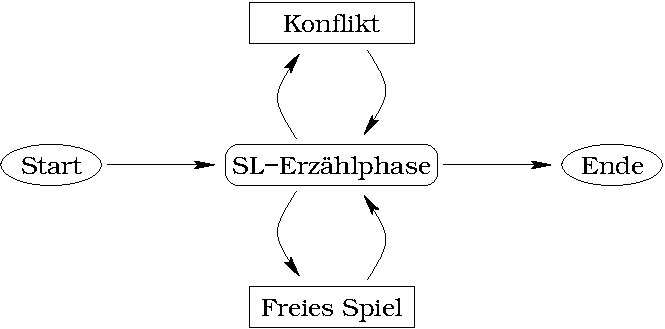
\includegraphics[width=0.8\textwidth]{pics/flowchart}}
\caption{Jedes Abenteuer beginnt und endet mit einer SL-Erzählphase. Dazwischen liegen immer wieder Konflikte und freies Spiel, wobei die Erzählphasen die Übergänge dazwischen darstellen.}

\medskip
\hrule
\end{figure}

Darüberhinaus gibt es noch \DEF{freies Spiel}\index{freies Spiel}, welches außerhalb von Konflikten steht. Dabei spielen die Spieler einfach in der gegebenen Szene die Charaktere frei aus. Hier können Entscheidungen über das weitere Vorgehen o.ä. entschieden werden.

Um eine klare Strukturierung des Spieles hinzubekommen, gibt es \DEF{Schlüsselworte}\index{Schlüsselworte} und Gesten. Damit leitet der SL von einer Phase zur nächsten über. Dazu sollte er sich -- falls er nicht die volle Aufmerksamkeit aller Spieler hat -- durch kurzes Räuspern oder Aufsetzen die Aufmerksamkeit sichern. Dann spricht er mit klarer Stimme und einer zur Stimmung passenden Stimme den Schlüsselsatz. So weiß jeder, in welcher Phase des Spiels man sich gerade befindet.

\subsection{Die Schlüsselworte in der Übersicht}
\begin{description}
\item[Freies Spiel:] ``Was wollt ihr tun?''

\item[Einleitung eines Konfliktes:] ``Es kommt zu Schwierigkeiten. Dein/Euer Ziel ist es, \dots''

\item[SL-Erzählphase:] ``Nachdem du/ihr \dots''. Zur Verdeutlichung, dass in eine SL-Erz"ahlphase "ubergeleitet wird, kann der SL zus"atzlich die Hand heben.
\end{description}


\subsection{Beispiele}
\begin{beispiel}
\paragraph{Beispiel 1:} Der SL m"ochte den Spielern Gelegenheit geben, das weitere Vorgehen zu planen. Dazu beschreibt er, wie sich die Helden eine Taverne betreten. \emph{``\dots Rauchgeschw"angerte Luft schl"agt euch entgegen. Die fast heruntergebrannten Kerzen an den W"anden k"onnen den Raum nur schwer erhellen und tauchen ihn in ein unwirkliches Licht. An den niedrigen Tischen sitzen kaum erkennbare, dunkle Gestalten. `In was sind wir jetzt hineingeraten', denkt ihr euch. Da dr"ohnt aus dem hinteren Teil des Raumes die Stimme des Wirts: `Heda, Fremde! Setzt euch doch. Ich habe hier hinten noch einen guten Tisch f"ur Euch!' Ihr nehmt dankend an und setzt euch. {\bfseries Was wollt ihr tun?}''}

\paragraph{Beispiel 2:} Die Spieler entscheiden sich im Laufe ihrer Planung, Haken-Hoss aufzusuchen und ihm geh"orig eins zu verpassen. Dazu hatten sie bereits ein Boot am Ufer versteckt, mit dem sie zur Insel "ubersetzen wollen. Der SL muss also zun"achst eine SL-Erz"ahlphase einleiten, die er nutzen will, "uberraschenderweise eine Kneipenschl"agerei einzuleiten, denn einer der G"aste hat die Helden belauscht und will sie von ihrem Vorhaben abbringen: \emph{``{\bfseries Nachdem ihr} beschlossen habt, Haken-Hoss aufzusuchen und eure Humpen geleert habt, steht ihr auf, als pl"otzlich ein Raunen durch den Raum geht. Das Kratzen von St"uhlen und Tischen, die zur Seite geschoben werden, erf"ullt die Taverne. \textbf{Es kommt zu Schwierigkeiten. Euer Ziel ist es,} heil aus der Kneipenschlägerei herauszukommen.''}

\paragraph{Beispiel 3:} Nach dem Kampf erz"ahlt der SL, wie die Helden auf dem Weg zu Haken-Hoss das bereit gelegte Boot benutzen um damit zur Insel "uberzusetzen. \emph{``\dots steigt ihr alle ins Boot und legt ab. Das Meer ist heute unruhig, das Boot l"asst sich nicht so einfach steuern, wie ihr gedacht habt. {\bfseries Es kommt zu Schwierigkeiten. Euer Ziel ist es,} ohne zu kentern am Ufer der Insel anzukommen. ''}
\end{beispiel}

\begin{design}
\subsubsection{Designanmerkung: Phasen und Schl"usselworte}

Der Vorteil einer klaren Trennung der verschiedenen Phasen liegt auf der Hand: Der Spielleiter beh"alt die Herrschaft "uber den Plot und kann genau vorgeben, in welchem Rahmen die Spieler ihre Charaktere ausspielen d"urfen.

Die Schl"usselworte wiederum dienen dazu, das Spiel so unauff"allig wie m"oglich zu strukturieren, um den Spielfluss m"oglichst wenig zu st"oren. Dadurch ist allen Beteiligten auch ohne Out-Time Anmerkungen immer klar, in was f"ur einer Art von Spiel sie sich gerade befinden: Macht der SL nur eine Anmerkung zum freien Spiel oder leitet er eine SL-Erz"ahlphase ein? Kommt jetzt ein Konflikt oder kann ich meinen Charakter frei ausspielen?
\end{design}

\begin{optional}
\section{Optional: Andere Schl"usselworte}

Es ist im Allgemeinen problemlos m"oglich, auch andere Schl"usselworte zu benutzen. Wahrscheinlich wird sich auch mit der Zeit ein eigener Stil einschleifen, so dass jeder Spieler immer genau wei"s, in welcher Phase sich das Spiel gerade befindet.
\end{optional}



\chapter{Erzählungen}\label{Ch:Erzaehlungen}\index{Erzählung}
\lettrine[findent=0.3em,nindent=0.2em]{E}{rzählungen} nehmen eine zentrale Rolle im Rollenspiel ein. Insbesondere in diesem Spiel kommt es aufs Erzählen an -- stimmungsvoll ausgespielte Konflikte sollen ja schließlich im Vordergrund stehen.

Um das zu erreichen, soll einerseits jeder Spieler das Recht bekommen, im vom Spielleiter gesteckten Rahmen alles das zu erzählen, was ihm Spaß macht. Andererseits sollen aber auch die anderen Spieler die Möglichkeite haben, ihre Meinung über das Erzählte zu äußern.

\section{Prinzip der Erzählte Wahrheit}
Dieses Prinzip gilt während des gesamten Spiels (mit einer kleinen Abweichung in den Kurzkonflikten). Es besagt:
\begin{quote}
Alles, was ein Spieler erzählt, passiert, sobald er es erzählt und genau so, wie er es erzählt.
\end{quote}

Das bedeutet, es gibt kein `ich versuche, dies oder jenes zu tun', sondern nur ein klares `ich tue dies oder jenes'. Es gibt auch keine Nachfrage beim Spielleiter, ob irgendetwas vorhanden ist oder ob etwas möglich ist oder nicht. Die Erzählte Wahrheit gilt unabhängig von irgendwelchen Würfelergebnissen.

Die Kurzkonflikte weichen von dem Prinzip dahingehend ab, dass zunächst gesagt wird, was der Charakter vorhat, dann wird gewürfelt und erst danach wird im Rahmen des Würfelergebnisses erzählt.

Insbesondere soll hier darauf hingewiesen werden, dass auch in den SL-Erzählphasen das Prinzip der Erzählten Wahrheit gilt. Allerdings gibt es hier (im Gegensatz zu den Konflikten und dem freien Spiel) kein persönliches Veto-Recht (s.\,u.), so dass der Spielleiter in seinen Erzählungen den Plot in die Richtung lenken kann, die er vorgesehen hat.

\section{Das Konfliktende}
Durch das Prinzip der Erzählten Wahrheit könnte ein Spieler gleich zu Beginn eines Problems das Ende beschreiben. Das wird aber durch die \DEF{Konfliktende}-Regel\index{Konfliktende} verboten.
\begin{quote}
  Bevor nicht das Ende eines Konfliktes erreicht ist, darf niemand das Ende vorwegnehmen.
\end{quote}
Das Ende eines Konfliktes wird, wie später noch erklärt wird, durch Würfelwürfe bestimmt. Ist das Konfliktende erreicht, darf die Gewinnerseite erklären, wie das Konfliktende aussieht. Dabei hat der SL aber immer das Recht, Ergänzungen in der dann folgenden SL-Erzählphase zu machen.

Konfliktende bedeutet jedoch nicht, dass z.\,B. am Ende eines Kampfes alle Gegner getötet werden müssen. Es kann auch sein, dass ein Überlebender gefangen wird, dass die Gegner alle vertrieben wurden, usw. Am Konfliktende steht also fest, wer gewinnt. Wie genau dieser Gewinn aussieht, kann der Gewinner des Würfelduells festlegen.

\section{Kompetenzen}
Damit das Spiel nicht ganz aus dem Ruder läuft, gibt es eine klare Kompetenzregelung, was die einzelnen Spieler erzählen dürfen. Das wichtige ist dabei, dass kein Spieler seine Kompetenzen überschreiten darf. Der Spielleiter hat in den SL-Erzählphasen, das Recht, die Geschichte beliebig weiter zu erzählen. Dabei darf er die Spielercharaktere genauso einbinden wie andere Charaktere oder die Umgebung. Auch Zeitsprünge o.\,ä. sind dem Spielleiter erlaubt.

Im freien Spiel hat jeder Charakterspieler die Kompetenz, die Handlungen seines Charakters zu beschreiben und eventuelle Details der Umgebung hinzuzufügen. Der Spielleiter hat im freien Spiel die Hoheit über alle Charaktere außer den Spielercharakteren, wobei er seine Kompetenz auch an andere Spieler abgeben darf.

In Konflikten haben alle Spieler die Kompetenz, einen beliebigen Verlauf des Geschehens zu erzählen, einschließlich aller Charaktere. Einzig die Konfliktende-Regel muss eingehalten werden.

\section{Veto}
Gegen jegliche Art von Erzählung während der Konflikte, des freien Spiels und der SL-Erzählphasen hat jeder Spieler ein allgemeines Veto-Recht. Setzt ein Spieler sein Veto ein, wird das Spiel angehalten. Dann wird darüber diskutiert, was dem Spieler an der Erzählung nicht gepasst hat und wie man das Problem beheben könnte. Anschließend wird die Erzählung wiederholt und das Spiel läuft normal weiter.

Das allgemeine Veto dient als eine Art Notbremse dazu, unpassende und stimmungstötende Beschreibungen zu unterbinden. Weiterhin kann damit das verfrühte Ende eines Konfliktes oder eine Kompetenzüberschreitung gestoppt werden. Das allgemeine Veto darf nicht dazu benutzt werden, eigene Ideen in die Beschreibung von anderen mit einzuflechten sondern dient ausschließlich dazu, andere Beschreibungen mit einer guten Begründung zu stoppen. 

In Konflikten hat jeder Spieler zusätzlich noch ein persönliches Veto, was bedeutet, dass jeder Spieler praktisch die Kontrolle über seinen eigenen Charakter behält (bzw. der Spielleiter über alle weiteren Spielfiguren). Dieses kann jeder Spieler einsetzen, um Beschreibungen zu stoppen, die ihm einfach nicht für diesen Charakter passend erscheinen. Für ein persönliches Veto ist eine Begründung wie `stimmungstötend' oder `Kompetenzüberschreitung' nicht nötig. Das Missfallen einer Beschreibung reicht schon.

Wichtig ist, dass die Vetos auch eingesetzt werden, d.\,h. ein Spieler sollte nicht etwas einfach so dulden, obwohl er ein Veto einsetzen könnte. Wenn das Veto auch wirklich benutzt wird, funktioniert die Veto-Regel nach einiger Zeit durch nicht-Anwendung, d.\,h. die Spieler werden eine bestimmte Tatsache, bei der sie sicher sind, ein Veto zu erhalten, einfach nicht erzählen.

\section{Erzählwert}
In Haupt- und Nebenkonflikten (nicht aber in Kurzkonflikten) wird der Fortgang des Konfliktes häppchenweise erzählt. Nach jedem Stück Erzählung wird der \DEF{Erzählwert}\index{Erzählwert} durch den SL festgelgt. Für jedes eingebrachte Faktum gibt es einen Würfel, bis maximal 5 Würfel. Dabei ist egal, ob die Fakten stimmig sind, gut zusammenpassen o.\,ä. Die Qualität spielt also keine Rolle, es zählt nur die Quantität. Was genau als Faktum zählt, liegt beim SL. Als Richtlinie gilt, dass jede Aktion und jede nähere Beschreibung mit einem Würfel belohnt werden soll.

Ist eine Beschreibung allzu abwegig und damit nicht hinnehmbar, so sollte ein Veto eingelegt werden. Für qualitativ besonders gelungene Beschreibungen können die Charakterspieler Erzählmarken (s.\,u.) vergeben.

Die Erzählwert-Regel dient dazu, die Menge der Erzählungen der Spieler zu steuern. Da ein einzelner Punkt leicht zu bekommen ist, kann man davon ausgehen, dass jede Erzählung immer den vollen Punktewert bekommt.

\subsection{Beispiele}
\begin{beispiel}
\begin{itemize}
\item ``Ich schlage mit meinem Schwert.'' gibt 1 Würfel.
\item ``Ich schlage mit meinem Schwert in einem weiten Bogen.'' gibt 2 Würfel
\item ``Ich schlage mit meinem Schwert in einem weiten Bogen in Richtung seines Halses.'' gibt 3 Würfel
\item ``Ich schlage mit meinem Schwert in einem weiten Bogen in Richtung seines Halses. Er duckt sich darunter weg.'' gibt 4 Würfel
\item ``Ich schlage mit meinem Schwert in einem weiten Bogen in Richtung seines Halses. Er duckt sich darunter weg, so dass mein Schwert nur in den Balken fährt.'' gibt 5 Würfel
\end{itemize}
\end{beispiel}

\begin{optional}
\section{Optional: Anderes Erzählwert-Maximum}

Im Laufe des Spiel kann sich herausstellen, dass das Maximum von 5 Würfeln für die Gruppe zu hoch oder zu niedrig ist. Es kann natürlich problemlos geändert werden, jedoch sollte der SL dann beachten, dass sich dadurch die Schwierigkeit von Neben- und Hauptkonflikten ändert, d.\,h. evtl. müssen dann auch die Konfliktpunkte der Konfliktgegner angepasst werden. Dabei gilt natürlich: Je höher das Erzählwert-Maximum ist, umso einfacher sind die Konflikte.
\end{optional}

\begin{optional}
\section{Optional: Ohne Erzählwert}

Möchten die Spieler selber nicht so viel erzählen, so kann man die Erzählwert-Regel auch einfach weglassen und stattdessen \emph{jegliche} Aktion mit fünf Würfeln belohnen, unabhängig von der Menge der Beschreibung.

Eine Anregung, gute Erzählungen zu liefern, wird damit immer noch durch die Erzählmarken und durch die Konfliktstruktur gegeben. Aber ich empfehle ausdrücklich, dem Erzählwert eine Chance zu geben und ihn zumindest einen Spielabend lang zu testen. Auch bislang sehr ruhige Spieler wachsen erfahrungsgemäß bei solchen Regeln oft über sich hinaus.
\end{optional}

\section{Erzählmarken}
Darüberhinaus kann jeder Charakterspieler pro Spielabend zwei \DEF{Erzählmarken}\index{Erzählmarke} für seiner Meinung nach besonders stimmungsvolle Beschreibungen an einen anderen Charakterspieler vergeben. Das kommt oft in Haupt- oder Nebenkonflikten vor, kann auch für ein besonders gelungenes freies Spiel oder eine gute Beschreibung für einen Kurzkonflikt sein. Für eine Beschreibung kann ein Charakterspieler höchstens eine Erzählmarke bekommen. Wollen mehrere Spieler gleichzeitig für eine Beschreibung eine Marke vergeben, so müssen sie sich einigen, wer sie vergibt. Unabhängig von der Länge der Erzählung beträgt der Erzählwert für etwas, wofür eine Erzählmarke vergeben wurde, immer dem Maximum.

Wichtig ist, dass diese Marke bei einem späteren Konflikt eingesetzt werden kann; pro Konflikt kann höchstens eine Marke eingesetzt werden. Eine eingesetzte Marke gibt einen Bonuswürfel für die gesamte Dauer eines Konfliktes und zwar unabhängig von der eingesetzten Fähigkeit.

Für einen laufenden Konflikt ist die Marke wertlos. Außerdem kann niemand mehr als zwei Erzählmarken haben. Weitere vergebene Marken verfallen einfach. Marken, die an einem Spielabend nicht vergeben wurden, verfallen ebenfalls.

Erzählmarken können gut durch Pokerchips dargestellt werden, wobei streng zwischen noch nicht vergebenen und bekommenen Marken unterschieden werden muss -- am besten durch unterschiedliche Farben.

\begin{design}
\subsubsection{Designanmerkung: Das Zusammenspiel der Erzählregeln}\label{DesignAnmerkungenZusammenspielErzaehlregeln}

Durch die gegebenen Regeln -- Prinzip der Erzählten Wahrheit, Konfliktende, Veto, Erzählwert und Erzählmarken -- wird eine Qualitätssicherung in Sachen Erzählung erreicht.

Das Prinzip der Erzählten Wahrheit gibt jedem Spieler die Möglichkeit, seine Vorstellung von Aventurien und seinem Charakter im Spiel auch wirklich umzusetzen und nicht durch irgendwen oder irgendwelche verteilten Punkte aktiv dauernd daran gehindert zu werden. Damit das aber nicht ausufert, gibt es die Konfliktende- und die Veto-Regel. Erstere verhindert, dass dem SL der Plot aus der Hand genommen wird, letztere sichert, dass kein Spieler für ihn unterträgliches Spiel dulden muss.

Durch den Erzählwert wird die Quantität der Erzählung, durch die Erzählmarken die Qualität der Erzählung gesichert. Während der Erzählwert ein Minimum an Erzählung vorgibt, können die Mitspieler durch die Erzählmarken klare Signale setzen, welche Art von Beschreibung sie gerne haben wollen. Durch die Kombination aus Erzählwert und Erzählmarken wird aber auch indirekt ein Maximum an Beschreibung vorgegeben: Zu langatmige, selbstdarstellerische Beschreibungen, die deutlich den maximalen Erzählwert überschreiten, werden wohl kaum durch Erzählmarken gewürdigt. Umgekehrt können besonders einfallsreiche, sehr kurze Beschreibungen zu einer Erzählmarke führen und damit ggf. auch zum maximalen Erzählwert aufgestockt werden.
\end{design}

\begin{optional}
\section{Optional: Dem SL die Zügel aus der Hand nehmen}\label{Optional:ZuegelAusDerHand1}

Mit ein paar regeltechnischen Handgriffen ist es auch möglich, dem SL die Zügel aus der Hand zu nehmen. Dazu erweitert man einfach das persönliche Veto der Charakterspieler auch auf die SL-Erzählphase. Die Erzählung des Konfliktendes legt man völlig frei in die Hand des Gewinners -- dieser kann dann erzählen, wie die Geschichte weitergeht und die nächste SL-Erzählphase beginnen. Sollten die Spieler den Konflikt gewinnen, so müssen sie auch nicht den Erfolg der Charaktere erzählen. Vielmehr kann das Ende auch ein Misserfolg der Charaktere darstellen.

Weiterhin gibt man auch dem SL zwei Erzählmarken zum Verteilen und die CS können auch dem SL Erzählmarken geben. Erzählmarken sollen nicht mehr unbedingt für gutes Erzählen vergeben werden, sondern für gute Ideen im Allgemeinen. Außerdem müssen diese dann \emph{sobald möglich} (also im laufenden oder im nächsten Konflikt) eingesetzt werden.
\end{optional}


\section{Tipps für gute Erzählungen}\label{TippsGuteErz}
Erzählungen während der Konflikte haben nur geringe Auswirkungen auf den Ausgang. Einzig das Talent, auf welches gewürfelt wird, wird durch die Beschreibung bestimmt. Der Rest dient nur dazu, Würfel und Erzählmarken zu bekommen. Damit ist man darin, was man jetzt tatsächlich erzählt, sehr frei.

Es ist also kein Risiko dabei, zu erzählen, wie der eigene Held in Bedrängnis gerät und wie es ihm gelingt, sich aus diser Lage durch ein schwieriges Manöver wieder zu befreien. Wichtig ist nur, dass die Beschreibung zum Spielstil der Gruppe und zur Situation passen und die erzählte Geschichte bereichern. Die Würfelwürfe sind davon absichtlich losgelöst, damit nicht eine spannende Stelle zur Sicherheit lieber langweiliger beschrieben wird. Trotzdem haben natürlich die Fähigkeiten der Helden erheblichen Einfluss auf den Konfliktausgang. Veto-Recht und Erzählmarken stellen die Qualität der Erzählung sicher (vgl. hierzu auch die Design-Anmerkungen auf Seite~\pageref{DesignAnmerkungenZusammenspielErzaehlregeln}).

Durch den Erzählwert neigen manche Spieler dazu, eine reine Aufzählung von Adjektiven zu machen, um die fünf Würfel voll zu kriegen. Dem sollen die folgenden Tipps entgegenwirken. Klarerweise können sie nicht alle gleichzeitig angewedet werden, sondern sollen für interessante Beschreibungen abwechselnd benutzt werden.

\begin{description}
  \pagebreak[3]
  \item[Perspektiven:]~
  \begin{itemize}
    \item Ich-Perspektive
    \item Perspektive des Konfliktgegners
    \item Perspektive einer dritten Person
    \item Zoom auf ein Detail
    \item Zeitlupe
  \end{itemize}
  \pagebreak[3]
  \item[Inhalte:]~
  \begin{itemize}
    \item Aktion des Charakters oder eines Konfliktgegners
    \item Misslungene Aktion des Charakters oder eines Konfliktgegners 
    \item Einbeziehung der Umgebung und anderer Konfliktteilnehmer
  \end{itemize}
  \pagebreak[3]
  \item[Art und Weise:]~
  \begin{itemize}
    \item Besonders schnell oder langsam sprechen
    \item Besonders laut oder leise sprechen
    \item absichtliche kurze Pause
  \end{itemize}
\end{description}

Dabei sollte die Beschreibung natürlich immer zur Stimmung der Situation und des Konfliktes passen. Klar, wenn der Charakter heimlich an einer Wache vorbeischleicht, wird man kaum absichtlich laut oder hektisch reden -- höchstens um spannende Akzente zu setzen.

\begin{beispiel}
Die folgenden Beispiele haben jeweils einen Erzählwert von mindestens~5:
\begin{itemize}
  \item {Der Fußboden knackt leise, als Harro ganz vorsichtig einen Schritt nach vorne mache. Erschreckt bleibt er stehen. [hörbares Einatmen, kurzes Luftanhalten] Hat die Wache ihn gehört?}

  \item Ich springe vor, schlage mit meinem Schwert dem Ork mit einem `Schack' den Kopf von den Schultern. Dabei rammt mir ein anderer von links sein Knie in die Seite. Ich breche röchelnd zusammen.

  \item {Der Goblin sieht aus dem Augenwinkel einen Lichtblitz -- doch zu spät. Ein Pfeil steckt plötzlich in seinem Hals, Blut sickert langsam aus der Einstichwunde. Langsam und ohne einen Laut von sich zu geben bricht der Goblin zusammen.}

  \item {Von einem Stuhl in den Bauch gerammt rutscht Alrik auf mich zu. Mit einem Hechtsprung bringe ich mich in Sicherheit, reiße den Schürhaken aus dem Feuer und gehe bedrohlich auf den nächstbesten Schläger zu.}

  \item Der Wirt schaut mich an: `Was willst du? Informationen über den roten Alrik? Unter zwei Dukaten läuft da gar nichts.' Ich krame in meinem Geldbeutel herum und ziehe eine goldene Münze hervor.

  \item Schon seit Stunden irren wir durch den Wald. Der Regen ist so stark, dass selbst das dichte Blätterdach keinen Schutz mehr bietet. Den Blick immer nach unten gerichtet, um nicht die deutlichen Schleifspuren zu verlieren, die die Räuber hinterlassen haben.

  \item {Travianes rechte Hand krallt sich am Felsvorsprung fest. Jede Muskel ist angespannt, die Adern des Handrückens treten bläulich hervor. Sie keucht -- um Haaresbreite wäre sie abgestürzt. Doch jetzt, da sie sich wieder gefangen hat, schiebt sie sich wieder weiter nach oben.}
\end{itemize}
\end{beispiel}



\chapter{SL-Erz"ahlphase}\label{Ch:SLErzaehlphase}\index{SL-Erzählphase}
\lettrine{E}{ine}
SL-Erz"ahlphase hat diverse Funktionen: Sie soll das Abenteuer einleiten und beenden, "Uberg"ange zwischen freiem Spiel und Konflikten schaffen und die Story voranbringen, indem der Spielleiter die M"oglichkeit hat, unwichtige Dinge, langweilige Reisen und andere uninteressante Begebenheiten einfach zu "uberspringen. Dabei soll der SL nat"urlich nicht zum Alleinunterhalter verkommen, sondern vielmehr in kurzen Worten die richtige Stimmung f"ur die kommende Szene schaffen und die Spieler m"oglichst schnell wieder ans Ruder zu lassen.

Eine gute SL-Erz"ahlphase greift zun"achst kurz den Punkt auf, an dem die letzte Szene geendet hat. Die wird "ublicherweise durch die Einleitung ``Nachdem du/ihr\dots'' begonnen. Zur Verdeutlichung hebt der SL eine Hand: Eine SL-Erz"ahlphase hat begonnen.

Dann folgt eine kurze "Uberleitung zur n"achsten Szene, in der der Spielleiter darauf eingeht, wie sich die Spielercharaktere verhalten und was vielleicht einige der weiteren Charaktere unternehmen. Eine Reise "uber mehrere Wochen ist hier genauso m"oglich wie ein kurzes Aufschauen oder ein Luft Anhalten seitens der Charaktere.

Eventuell kann er auch eine Blende zu anderen Charakteren an einer anderen Stelle machen, so z.\,B. auf die Tochter des Barons, die gerade in Ketten in irgendeinem Kerker schmort oder zum Hexenzirkel, der sich gerade im Schutze der Nacht trifft. Solche Elemente k"onnen, wenn sie geschickt eingesetzt werden, die Spannung der Geschichte erh"ohen. Andererseits versorgt man die Spieler mit Wissen, dass die Charaktere nicht haben. Das st"ort manche Spieler und sollte unbedingt mit der Gruppe abgekl"art werden.

Zuletzt kommt der Rahmen der neuen Szene: Wo findet die n"achste Szene statt? Wer ist alles daran beteiligt? Was ist das Ziel der Charaktere oder was sind die offen stehenden Optionen? Hierbei sollte der Spielleiter den Ort, soweit er den Spielern noch nicht bekannt ist, kurz umrei"sen.



\chapter{Freies Spiel}\label{Ch:FreiesSpiel}\index{freies Spiel}
\lettrine{I}{m} freien Spiel können die Spieler nach Herzenslust ihre Charaktere ausspielen. Der SL hat zuvor durch eine SL-Erzählphase dazu die Rahmenbedingungen, wie Ort und anwesende Charaktere, geschaffen. Dann leitet er das freie Spiel mit den Schl"usselworten ``Was wollt ihr machen?'' ein.

Freies Spiel bringt die Story zwar nicht direkt voran, hilft aber, den gemeinsamen Vorstellungsraum auszuschmücken und den Spielern ein besseres `Gefühl' für ihren Charakter zu geben. Auch sollen im freien Spiel Planungen für das weitere Vorgehen gemacht werden oder auch Entscheidungen getroffen werden, wohin sich die Charaktere als nächstes wenden wollen. Hier können die Spieler auch durch ihre Gespräche und Handlungen dem SL Hinweise geben, was sie sich für ihre Charaktere wünschen.

Wichtig: Freies Spiel beinhaltet niemals Konflikte. Natürlich dürfen sich Charaktere im freien Spiel auch eins reinhauen o.\,ä. Diese `Konflikte' werden aber -- wenn sich die Spieler nicht einigen können -- durch den SL aufgelöst und haben keinerlei regeltechnischen Einfluss (auf Charakterwerte usw.). Der SL sollte in solchen Fällen aufgrund des Spielspaßes und der Charakterwerte entscheiden.

Der Spielleiter hat das Recht, das freie Spiel jederzeit zu unterbrechen. Dann kann er mit einer SL-Erzählphase z.\,B. zu einem Konflikt "uberleiten. Das sollte er insbesondere dann machen, wenn die Spieler im freien Spiel versuchen, die Story voran zu treiben und an eine Stelle gelangen, an der ein Konflikt vorgesehen war. Auch kann der SL damit verhindern, dass die Spieler etwas unternehmen, was im Plot nicht vorgesehen ist und kann sie mit einer SL-Erzählphase wieder zur"uck ``auf den rechten Weg'' bringen. Meist wird der SL aber allzu ausschweifende (und auf die Dauer langweilige) Charakter- bzw. Spielerdiskussionen unterbrechen um die Geschichte weiter zu f"uhren.



\chapter{Konflikte}\label{Ch:Konflikte}\index{Konflikt}
\lettrine[findent=1em,lraise=0.1]{K}{onflikte} sind das Salz in der Suppe eines Rollenspiels und sollten neben freiem Rollenspiel auch den Großteil einer Sitzung ausmachen. Mit Konflikten wird die Geschichte vorangetrieben, für die Helden steht etwas auf dem Spiel. Daher wird durch Konflikte das Spiel spannend.

Mit Konflikten ist jetzt nicht gemeint, dass es sich dabei zwangsweise um einen Kampf handelt. Konflikte sind alle Situationen, in denen (objektiv gesehen) nicht von vorne herein klar ist, ob das gewünschte Ergebnis eintritt. Also praktisch alles, wofür man normalerweise bei DSA einen Würfelwurf macht, ist ein Konflikt.

Ein Konflikt kann das Umgehen einer Wache sein (durch Schleichen, Bestechung oder auch durch von hinten niederstechen), es kann eine Verfolgungsjagd sein oder auch das Suchen von Informationen in einer Bibliothek. Aber natürlich ist auch ein schnöder Kampf ein Konflikt.

Bei Konflikten sollte der Spielleiter immer nur das Ziel vor Augen haben, nie aber die Methode. Im Beispiel oben habe ich ja auch angedeutet: eine Wache kann auf die verschiedensten Arten umgangen werden, wichtig ist für die Geschichte am Ende nur, ob das Ziel erreicht wurde oder nicht.

Außerdem muss sich der Spielleiter über die Rolle, die ein anstehender Konflikt spielt, Gedanken machen. Ist es ein Konflikt, der auf dem Weg zum Abenteuerende steht? Ist es wichtig, dass die Helden das Ziel erreichen? Wenn ja, dann sollte er den Konflikt als Nebenkonflikt modellieren. Ist hingegen der Konflikt ein Scheideweg für die Protagonisten oder ist sowohl das Gewinnen als auch das Verlieren eines Konfliktes interessante Optionen, sollte der Meister daraus einen Hauptkonflikt machen.

\section{Relevante Talente, Sonderfertigkeiten und Gegenstände}
In einem Konflikt kann im Prinzip jegliche Art von Talent benutzt werden. Dennoch gibt es Talente, die für einen Konflikt relevant sind und andere, die es nicht sind. Im Zweifelsfall entscheidet der Spielleiter, ob ein Talent in einem Konflikt relevant ist. Nur, wenn der Charakterspieler ein relevantes Talent einsetzt, darf er für den Konfliktausgang würfeln.

\begin{beispiel}
Beispiele für relevante Talente:
\begin{itemize}
  \item Eine Mauer erklimmen: Athletik oder Körperbeherrschung
  \item Der hübschen Wirtstochter Informationen entlocken: Betören, Überreden, Zechen, Tanzen, Singen
  \item Die Orkbande töten: alle Arten von Kampftalenten
\end{itemize}
\end{beispiel}

Zu den Talenten kann der Spieler eventuell noch passende Sonderfertigkeiten wählen. Pro Talent darf der Spieler aber nicht mehr als je eine offensive und eine defensive Sonderfertigkeit (das können auch aufgestockte Sonderfertigkeiten sein) einbringen. Sonderfertigkeiten geben immer die Möglichkeit zu einem meisterlichen Wurf.

Auch ist die Verwendung von Gegenständen erlaubt und gibt zusätzliche Würfel oder sogar automatische Erfoge. Üblicherweise kann aktiv nur ein Gegenstand eingesetzt werden (z.\,B. eine Waffe). Wirken Gegenstände passiv, so können diese zusätzlich benutzt werden (z.\,B. eine Rüstung oder ein Schild).

Um die Boni von Sonderfertigkeiten oder Gegenständen zu bekommen, müssen diese in den Beschreibungen mit einfließen. Dabei reicht es aber, wenn der Spieler das nur implizit erwähnt. Beispielsweise kann ein Charakter in der ersten Runde sein Schwert ziehen. Wenn der Spieler dann in der nächsten Runde beschreibt, wie der Charakter zuschlägt, kann man davon ausgehen, dass er das mit dem gezogenen Schwert tut.

Natürlich muss ein Charakter nicht immer während des gesamten Konfliktes dasselbe Talent mit denselben Sonderfertigkeiten und denselben Gegenständen einbringen. Das hängt immer von der Beschreibung ab, die die Spieler liefern. Die Nutzung von mehreren Talenten gleichzeitig ist jedoch nicht möglich.

Andererseits sind auch nicht unbedingt während des gesamten Konfliktes immer dieselben Talente relevant: Sollte z.\,B. eine Diskussion kippen und in einer Schlägerei enden, so ist Überreden/Überzeugen anfangs noch interessant, nachdem aber erst einmal die Fäuste fliegen ist es nicht mehr sehr angebracht. Wie immer liegt das im Ermessen des Spielleiters.

\section{Ziele}
Im normalen DSA-Spiel bleiben die Ziele, zu denen ein Konflikt aus Sicht der Helden führen soll, meist unerwähnt. Als Beispiel betrachte ich einmal einen typischen Grund für eine Probe, wie sie normalerweise bei DSA gemacht wird: `Schaffe ich es, über die Mauer zu klettern?' Klar: Es wird auf Athletik gewürfelt und je nach Probenausgang ist die Aktion gelungen oder auch nicht (oder sie ist, wenn der Meister es so entscheidet, nur halb gelungen, auf das Ergebnis kommt es hier aber nicht an). Ist die Probe misslungen, so versucht es der Spieler entweder nochmal oder er probiert was anderes. Z.\,B. die Frage: `Schaffe ich es, mit meiner Spitzhacke ein Loch in die Mauer zu machen, so dass ich da durch passe?'

Und genau das ist der Punkt: Eigentlich geht es doch normalerweise gar nicht darum, über die Mauer zu klettern. Normalerweise geht es darum, die Mauer zu überwinden, und dabei spielt die Methode nur eine untergeordnete Rolle. Im normalen DSA-Spiel wird immer Methode und Ziel miteinander verknüpft. Im Beispiel ist das (ungenannte) Ziel: `Schaffe ich es, die Mauer zu überwinden?' Und diese Frage wird zunächst fest mit der Methode `Klettern', dann im zweiten Versuch mit der Methode `Hacken' verbunden. Es gibt natürlich noch viele andere Methoden und das normale DSA-Spiel geht davon aus, dass der Spieler alle diese Methoden hintereinander ausprobiert, bis eine Methode gelingt.

In diesem Spiel steht aber zunächst immer die Frage nach dem eigentlichen Ziel im Vordergrund. Was will der Spieler bzw. sein Held erreichen? Wo will er wirklich ankommen? Und genau das wird als \DEF{Ziel}\index{Ziel}\index{Konfliktziel|see{Ziel}} bezeichnet. Manchmal ist auch das Gelingen einer Methode das Ziel (z.\,B. ein Schwertkampf auf einem Ritterturnier; da geht es darum den Gegner mit dem Schwert zu besiegen), aber das ist eher die Ausnahme.

Während des Konfliktes werden (wenn es nicht ein Kurzkonflikt ist) mehrere Würfe gemacht und durch die Erzählte Wahrheit kann jeder Spieler den Weg versuchen, den geeigneten Weg zur Hindernisüberwindung zu wählen. Daher ist es wichtig, wirklich das Ziel und nicht vor allem die Methode vor Augen zu haben.

\section{Schaden}\label{Schaden}\index{Schaden}
Während der Konflikte kann ein Charakter \DEF{Schaden}\index{Schaden} bekommen. Wie viel Schaden genau vergeben wird, wird bei den einzelnen Konfliktarten beschrieben. Dabei ist mit Schaden nicht ausschließlich eine Wunde gemeint -- Schaden kann es auch durch Gespräche, Stress u.\,ä. geben. Grundsätzlich gibt es zwei Arten von Schaden: \DEF{Körperlichen}\index{Schaden!körperlich} und \DEF{geistigen Schaden}\index{Schaden!geistig}.

Der Schaden wird immer nach Ablauf eines Konfliktes bestimmt. Dabei gilt: Je länger ein Konflikt andauert, umso größer ist im Mittel der verursachte Schaden. Für jede Runde, die ein Konflikt andauert, und jeden verlorenen Konfliktpunkt wird 1W20 geworfen. Jeder Würfel, der 9 oder mehr (Nebenkonflikte\index{Nebenkonflikt}) bzw. 5 oder mehr (Hauptkonflikte\index{Hauptkonflikt}) zeigt, ergibt einen Schadenspunkt.

Kurzkonflikte sind hier relativ ungefährlich. Nur, wenn Schaden auch wirklich auf dem Spiel steht, können Charaktere durch einen verlorenen Konflikt Schaden bekommen. 

Welche Art von Schaden gemacht wird, geht aus dem Zusammenhang hervor. Körperlicher Schaden\index{Schaden!körperlich} sind z.\,B. Verletzungen oder Schmerzen durch äußere Gewalteinwirkung. Geistiger Schaden\index{Schaden!geistig} hingegen kann sich in Ungeduld, Unaufmerksamkeit, Schamgefühl, Angst usw. äußern. Im Zweifelsfall legt der Spielleiter die Art des Schadens fest.

\section{Konfliktausgang}\index{Konfliktausgang}
Gewonnene Konflikte haben (außer evtl. Schaden) niemals negative Auswirkungen für die Helden. Ist ein Konflikt gewonnen, heißt das, das die Helden ihr Ziel\index{Ziel} erreicht haben.

Bei verlorenen Konflikten müssen Haupt-, Nebenkonflikte und Kurzkonflikte unterschieden werden. In Kurz-\index{Kurzkonflikt} und Nebenkonflikten\index{Nebenkonflikt} sollten folgende zwei Regeln beachtet werden:
\begin{enumerate}
\item[\#1:] Die beteiligten Charaktere versagen nicht auf ganzer Linie.
\item[\#2:] Der Misserfolg sollte einen weiteren Konflikt nach sich ziehen.
\end{enumerate}
Das bedeutet jetzt nicht, dass die Helden in Nebenkonflikten nicht versagen können. Es ist problemlos möglich, dass sie ihr Ziel nicht erreichen -- das kommt ganz auf den SL und die geplante Geschichte an. Jedoch sollen die Charaktere in Nebenkonflikten nicht entgültig verlieren und es muss eine plausible Möglichkeit geben, wie die Geschichte weiter verläuft. Aber: Misserfolge sollen den Helden größere Probleme einbringen, wenn möglich \DEF{Folgekonflikte}\index{Folgekonflikt}. Dabei handelt es sich einfach um Konflikte, die sich daraus ergeben, dass ein Konflikt verloren wurde. Folgekonflikte sind niemals wichtiger als ihre Ursache, d.\,h. ein Folgekonflikt zu einem Nebenkonflikt ist entweder wieder ein Nebenkonflikt oder ein Kurzkonflikt, aber kein Hauptkonflikt.

Misslungene Hauptkonflikte\index{Hauptkonflikt} bedeuten einen ernsthaften Verlust auf der Seite der Charaktere. Das kann der Tod eines Helden sein, aber auch einfach das Scheitern an der gestellten Aufgabe. So beendet ein verlorener Hauptkonflikt üblicherweise nicht das gesamte Spiele. Der Ruhm der Helden wird jedoch nicht zunehmen, so dass es für diesen Teil des Spieles dann keine Abenteuerpunkte gibt.

\section{Wiederholung von verlorenen Konflikten}\index{Wiederholung}

Als Spieler könnte man auf die Idee kommen, einen verlorenen Konflikt zu wiederholen um ein verfehltes Ziel doch noch zu erreichen. Das ist aber nicht so ohne weiteres möglich. Ein verlorener Konflikt bedeutet, dass der Charakter alles versucht hat, sein Ziel zu erreichen. Es ist nicht so, dass nur der erste Versuch danebengegangen ist, sondern dass alle Möglichkeiten ausgereizt wurden.

Daher muss sich an den Umständen, die zum Ziel führen, etwas wesentlich anders sein. So kann der Held z.\,B. Unterstützung durch seine Kameraden bekommen, der Konflikt findet an einem völlig anderen Ort statt oder es hat sich etwas anderes grundlegend an den Voraussetzungen geändert.

Außerdem muss eine Wiederholung auch von den äußeren Umständen her erlaubt sein. So bedeutet ein verlorener Konflikt für einen Verfolgten zumeist, dass er eingeholt wurde. Dass man diesen Konflikt dann auf keinen Fall wiederholen kann (höchstens durch einen erneuten Fluchtversuch) versteht sich von selbst.

\begin{beispiel}
\textbf{Beispiele:}
\begin{itemize}
  \item Ein zweiter Athletik-Konflikt (bei demselben Hindernis) steht einem Helden z.\,B. dann zu, wenn er es besser ausgerüstet erneut versucht oder wenn sich der Athletik-Talentgesamtwert in der Zwischenzeit verbessert hat.

  \item Um eine Person doch noch zur Herausgabe eines wichtigen Gegenstandes zu bewegen, kehrt der Held mit seinen Freunden zur Unterstüzung zurück.
\end{itemize}
\end{beispiel}

\begin{design}
\subsubsection{Designanmerkung: Konfliktwiderholungen}
Warum kann man nicht einfach einen Konflikt nochmal auswürfeln? Das hat zwei Gründe:
\begin{enumerate}
  \item Die Konflikte werden dadurch für die erzählte Geschichte bedeutend. Ein verlorer Konflikt hat Auswirkungen, ein Konflikt ist immer ein wichtiges Ereignis. Umgekehrt wird so der Spielleiter dazu gezwungen, sich zu überlegen, ob tatsächlich ein Konflikt vorliegt oder ob es nur darum geht, den Spieler nochmal würfeln zu lassen. Vor allem auch die Auswirkungen eines Konfliktes müssen überlegt sein, denn wie langweilig wäre ein verlorener Konflikt, der keine Auswirkungen hat?
  \item Würfelorgien werden vermieden. Oft passiert es im klassischen Spiel, dass die Spieler z.\,B. eine Suchen-Probe so oft wiederholen, bis sie etwas gefunden haben. Da wäre es doch besser von Anfang an zu beschreiben, wie der Charakter den gesuchten Gegenstand findet, ohne das Spiel durch eine Probe zu unterbrechen.
\end{enumerate}
\end{design}



\section{Kurzkonflikt}\index{Kurzkonflikt}\label{Sec:Kurzkonflikt}
Kurzkonflikte sind noch `unwichtiger' als Nebenkonflikte, d.\,h. im wesentlichen sind es Schwierigkeiten, die überwunden werden sollten oder keine entscheidende Auswirkung auf die Geschichte haben. Geeignet für Kurzkonflikte sind Situationen, die schnell wieder vorbei sind oder solche, die zwar länger dauern aber in ihrem Verlauf prinzipiell nicht besonders interessant sind. Eine weitere Anwendung ergibt sich in Situationen, die gut ausgespielt werden können und bei denen viel Würfelei nur stört. In jedem Fall sollte nur ein Spielercharakter am Konflikt beteiligt sein bzw. jeder SC muss die Situation individuell meistern.

\begin{design}
\subsubsection{Designanmerkung: Wozu Kurzkonflikte?}
Kurzkonflikte sind von den Regeln her vor allem für die Anwendung von Heilungstalenten vorgesehen. Das Wiederherstellen der Spielercharaktere ist ein für DSA typischer Vorgang und passt auch gut zu den Abenteuern, die üblicherweise gespielt werden. Trotzdem wären Nebenkonflikte für die Heilung zu aufwändig und nähmen zu viel Spielzeit ein. Die Heilungs-Kurzkonflikte stellen außerdem sicher, dass es eine Nische `Heiler' gibt, die von einem Charakter besetzt werden kann.

Aus ähnlichen Gründen kann der Spielleiter Kurzkonflikte im Spiel einsetzen: Das ausführliche Ausspielen eines Konfliktes zu einem bestimmten Talent könnte im Spiel als zu langweilig empfunden werden. Wenn ein Spieler das Talent trotzdem gesteigert hat, kann der Spielleiter dies über Kurzkonflikte wichtig machen, ohne das im Spiel auszubreiten.

Eine weitere Möglichkeit für Kurzkonflikte ist, sie als Weiche für verschiedene Wege zu benutzen. So könnte der einfachere Weg den Charakteren dann offenstehen, wenn ein bestimmter Kurzkonflikt gewonnen wurde. Eine typisches Beispiel hierfür ist Fährtensuchen: Gelingt der Kurzkonflikt, so gelingt die Verfolgung ohne Probleme, misslingt dagegen die Probe, so folgt ein Kampf, weil die Charaktere von der Ideallinie abweichen und in einen Hinterhalt geraten.
\end{design}

Ob ein relativ unwichtiger Konflikt als Kurz- oder Nebenkonflikt ausgespielt wird, entscheidet der SL, wobei er dabei Rücksicht auf die Wünsche der Spieler nehmen soll.

\begin{beispiel}
\paragraph{Einige Beispiele:}
\begin{description}
\item[Kurze Handlungen:] Taschendiebstahl, sich verstecken, etwas werfen, jemanden hinterrücks erstechen
\item[Langweilige Handlungen:] Klettern, auf Lauer liegen, die Bibliothek durchsuchen
\item[Gut ausspielbar:] Streitgespräche, Bestechungen
\end{description}
Dabei kann natürlich etwas, was hier als `kurz' oder `langweilig' beschrieben ist, in der konkreten Situation lang oder besonders interessant sein (z.\,B. wenn der Taschendieb einen für die Story wichtigen Gegenstand klauen will). Aber in vielen Fällen lohnt in diesen Punkten das Ausspielen als Kurzkonflikt.
\medskip
\end{beispiel}

Wichtig ist bei Kurzkonflikten, dass die Aktivität immer vom Helden ausgeht. Der Held muss etwas schaffen, der SL würfelt in solchen Situationen nie. Wenn sich die Helden versuchen, an einem Wachmann vorbeizuschleichen: Die Charakterspieler müssen Schleichen würfeln. Wenn sich ein Räuber versucht, an einem Helden vorbeizuschleichen: Die Charakterspieler müssen Sinnenschärfe würfeln.


\subsection{Ablauf}\label{KurzkonfliktAblauf}\index{Kurzkonflikt!Ablauf}

\begin{enumerate}
  \item Zuerst wird vom SL (bzw. von allen Spielern gemeinsam) das Konfliktziel festgelegt. Also: Was soll erreicht werden? Dabei soll das \emph{Ergebnis} im Vordergrund stehen, nicht, auf welche Weise es der Charakter erreichen soll. Weichen die möglichen Folgen eines verlorenen Kurzkonfliktes vom Nichterreichen des Zieles ab, so muss dies hier auch vom Spielleiter angesagt werden. Eines der wichtigsten Beispiele hierfür ist, dass der Charakter durch den Ausgang eines Kurzkonfliktes Schaden nehmen könnte.

  \item Dann wählt der Spieler aus, mit welchem Talent oder Zauber der SC das Ziel erreichen soll; dazu legt der SL dann die Schwierigkeit fest. Normalerweise sind alle Aufgaben `normal schwierig'. Nur, wenn die äußeren Umstände widrig sind, kann es einen Schwierigkeit von $+3$ oder $+6$ (besonders widrig) geben. Besonders günstige Umstände können die Probe auch vereinfachen (Schwierigkeit $-3$). Die Schwierigkeit soll alleine für die Umstände, nicht für das Ziel an sich vergeben werden.

  \begin{beispiel}
    \paragraph{Beispiel:} Eine steile Wand zu erklimmen erfordert eine Athletik-Probe. Das ganze ohne Seil oder im stürmischen Regen ergibt eine Athletik-Probe $+3$. Ohne Seil im stürmischen Regen dagegen ist $+6$.
  \end{beispiel}

  Konflikte, von denen der SL meint, sie seien für den Charakter nicht zu gewinnen, sind automatisch verloren (automatischer Misserfolg). Sollte die Schwierigkeit nicht $0$ betragen oder sogar die Probe unmöglich zu schaffen sein, so muss der SL dies ansagen.

  \item Wenn dem Spieler die Vorgaben vom SL zu risikoreich erscheinen, kann er sich noch entscheiden, ein anderes Talent zu benutzen (und hoffen, dass der Konflikt damit einfacher zu gewinnen ist) oder dem Problem ganz aus dem Weg gehen. Das Ergebnis wird in diesem Fall vom SL festgelegt. Dieser \emph{kann} auch entscheiden, dass das aus dem Weg gehen keine Option für den Charakter darstellt.
  
  \item\label{KKAbschnittWuerfeln} Jetzt wird mit W20 gewürfelt. Hat der Spieler mehr als einen Würfel zur Verfügung {(vgl. auch den Abschnitt ``Bonuswürfel'' ab Seite \pageref{Bonuswuerfel})}, zählt für das grundsätzliche Gelingen oder Misslingen erstmal nur das niedrigste Ergebnis. Dazu wird jetzt die Schwierigkeit addiert. Ist das Ergebnis höchstens der Talentgesamtwert, so ist die \DEF{Probe gelungen}\index{Probe!gelungen}, der Charakter hat einen \DEF{Erfolg}\index{Erfolg}. Ist das Ergebnis über dem Talentgesamtwert, ist die \DEF{Probe misslungen}\index{Probe!misslungen}, der Charakter hat einen \DEF{Misserfolg}\index{Misserfolg}.
  
  Wenn das Ergebnis gelungen ist \emph{und} das kleinste Würfelergebnis höchstens 1 zeigt, so könnte ein kritischer Erfolg vorliegen. Sollte der Charakter über eine passende Sonderfertigkeit verfügen, so reicht es aus, wenn das Würfelergebnis im Bereich 1--2 (bzw. 1--4 bei einer aufgestockten Sonderfertigkeit) liegt. In diesem Fall ist der \DEF{Erfolg kritisch}\index{Erfolg!kritisch}.

  Wenn das Eregebnis misslungen ist \emph{und} das größte Ergebnis 20 zeigt, so liegt ein \DEF{kritischer Misserfolg}\index{Misserfolg!kritisch} vor.

  \item Als letztes geht es ans Erzählen des Konfliktausgangs. Hierzu gibt es weitere Informationen im nächsten Abschnitt.
\end{enumerate}

\subsection{Konfliktfolgen}
 Das genaue Ende des Konfliktes legt der Spielleiter fest: Entweder, er erzählt es selbst, oder er erklärt seine Idee und spielt es dann zusammen mit den Spielern aus. Haben die Spieler gewonnen, legt der Spielleiter positive Folgen fest. Haben sie dagegen verloren, legt er die Folgen des Scheiterns fest. Wie schon geschrieben, dürfen die Charaktere aufgrund eines Kurzkonfliktes nicht auf ganzer Linie verlieren, auch wenn ein verlorener Konflikt natürlich negative Folgen haben sollte.

Der Spielleiter kann natürlich die Ausschmückung des Konfliktendes auch dem Spieler überlassen. Dabei sollte er aber darauf achten, dass ihm das Ruder der Geschichte nicht aus der Hand gleitet.

Als Richtlinie für Schaden und andere Konfliktfolgen soll folgende Liste gelten:

\begin{description}
  \item[kritischer Misserfolg] Es passieren katastrophale oder lustige Dinge -- hier kann der Spielleiter seiner Phantasie freien Lauf lassen, um ein besonders lustiges, spannendes oder dramatisches Probenende zu erzählen. Es kann sein, dass das Konfliktziel dennoch mit Mühe und Not erreicht wird. In diesem Fall folgt normalerweise ein knackiger Folgekonflikt.
  
  Vorher angesagter Schaden wird verdreifacht.

  \item[Misserfolg] Der Spielleiter erzählt den Konfliktausgang. Dabei wird das Konfliktziel häufig dennoch erreicht, jedoch kommt es zu Problemen. Normalerweise folgt auf einen Misserfolg, bei dem der Charakter das Konfliktziel dennoch erreicht, ein weiterer Konflikt. Der Spielleiter kann auch entscheiden, dass das Konfliktziel nicht erreicht wird.
  
  Vorher angesagter Schaden tritt ein.

  \item[Erfolg] Das bedeutet, dass der Konflikt erfolgreich gemeistert wurde, das Ziel wurde ohne größere Probleme erreicht.

  \item[kritischer Erfolg] Der Charakter erreicht sein Ziel grandios. Der Spielleiter darf besonders spektakulär ausschmücken, wie der Charakter alle Schwierigkeiten überwindet.
\end{description}

\subsection{Beispiele}

\begin{beispiel}
\paragraph{Beispiel 1:} Der SL beschreibt (SL-Erzählphase), wie die Flucht des Helden durch eine ihm unbekannte Stadt plötzlich in einer Sackgasse vor einer Mauer endet. Es kommt zum Kurzkonflikt: Kann der Held die Mauer überwinden?

Damit ist Punkt~1 des Ablaufes (vgl. Seite~\pageref{KurzkonfliktAblauf}) schon abgehandelt -- auch ohne, dass ein Wort gewechselt werden muss. Es ist klar, das der Charakter weiter fliehen will, da die ihn verfolgende Übermacht zu groß ist. Der Spieler sagt: ``Ich versuche, über die Mauer zu klettern''. Da es keine widrigen Umstände gibt, beträgt die Schwierigkeit 0 und der SL sagt nur ``Ok, wenn die Probe misslingt, bekommst du 2 Punkte Schaden. würfle.'' (Punkt 2) Die Punkte 3 und 4 werden dann auch schnell abgehandelt: Der Spieler hat als offensive Sonderfertigkeit `Einbrechen' gewählt, was ihm einen meisterlichen Wurf auf Athletik, Schlösser knacken, Körperbeherrschung und Fallen entschärfen ermöglicht; in Klettern hat er einen Gesamtwert von 12. Er darf also einen W20 benutzen und würfelt eine 20, also misslungen, da die Zahl größer als 12 ist. Da der Würfel aber sogar eine 20 zeigt, könnte das einen kritischen Misserfolg nach sich ziehen. Also nachwürfeln: 12. Knapp gelungen, also war es nicht kritisch, trotzdem aber misslungen.

So erzählt der SL (Punkt 6): ``Beim Versuch, die bestimmt drei Schritt hohe Mauer zu überwinden, rutscht du ab und schürfst dir deinen rechten Arm auf (d.\,h. der erhaltene Schaden ist körperlich). Die Verfolger biegen um die Ecke und sind schon in Sichtweite, als es dir unter Schmerzen endlich gelingt, dich über die Mauer zu ziehen. Du hetzt weiter und siehst dich um: Auch die Verfolger haben es über die Mauer geschafft!''

Jetzt schließt sich ein Folgekonflikt an.

\paragraph{Beispiel 2:} Die Streunerin Adessa der Gruppe soll sich in der zwielichtigen Gesellschaft umhören, wo sie die Diebesbande 'Goldener Handschuh' finden kann. Im freien Spiel entscheiden die Spielerinnen, dass sie sich in einer Taverne im Hafenviertel umhören soll. Sie betritt also die Taverne und trifft dort auf den schmierigen Wilbur. Das Ziel der Streunerin ist klar: ``Herausfinden, wo der Goldene Handschuh zu finden ist''.

``Den betöre ich.'', sagt die Spielerin. Da Wilbur fett, hässlich und schmierig ist hat er schon lange keine Frau mehr gehabt, also entscheidet der SL, dass dies vereinfachende Umstände sind (Schwierigkeit $-3$). Adessa hat in Betören/Galanterie einen Gesamtwert von 10 und kann keine Sonderfertigkeit einbringen. Sie würfelt also 1W20: 3. Das Ergebnis ist damit 0 (wegen der Schwierigkeit), also könnte der Erfolg sogar kritisch sein. Erneuter Wurf: 12, macht 9, also ist die Probe kritisch gelungen!

Da die Probe gelungen ist, wird Adessa die Information durch ihre Betörungskünste bekommen. Durch ihren grandiosen Erfolg schafft sie es sogar, Wilbur dann die versprochene Bettpartie wieder auszuschlagen, ohne dass dieser sauer auf sie wird.

\paragraph{Beispiel 3:} Die Spielgruppe ist im freien Spiel, das Nachtlager ist gerade aufgeschlagen worden. Die Helden beschließen, jagen zu gehen. Da es sich hierbei nicht um einen Konflikt handelt, der die Story irgendwie weiterbringt, beschreibt der SL oder der Spieler (je nach Präferenz der Gruppe) kurz den Jagderfolg des Jägers und fährt dann mit dem Konflikt der Nachtwache fort. Es kommt zum Konflikt: Schafft es der gerade wachhabende Held, den sich anschleichenden Räuber zu bemerken?
\end{beispiel}

\subsection{Gegenseitige Hilfe}
Möchte ein Charakter einen anderen bei der Ausführung seines Kurzkonfliktes unterstützen, so muss er dies ansagen, \emph{bevor} der Spieler würfelt, aber nachdem sich der Spieler festgelegt hat, welches Talent er benutzen will (also im Ablauf direkt vor Abschnitt~\ref{KKAbschnittWuerfeln}). Der Spieler muss beschreiben, auf welche Weise sein Charakter helfen möchte.

Der ursprüngliche Kurzkonflikt wird dann unterbrochen und ein neuer Kurzkonflikt zur Hilfe wird begonnen, mit allen Konsequenzen für den Helfenden. Geligt der Kurzkonflikt, so wird der ursprüngliche Konflikt um 3 erleichtert. Misslingt die Hilfe, so passiert nichts, misslingt die Hilfe jedoch kritisch, so wird der ursprüngliche Konflikt um 3 erschwert.

Auf diese Weise kann einem Charaker theoretisch von beliebig vielen anderen geholfen werden. Die Hilfe muss allerdings plausibel erklärbar sein. Als Richtlinie soll hier aber festgehalten werden, dass wenn zwei oder mehr Charaktere einen weiteren bei einem Kurzkonflikt unterstützen wollen, sollte besser ein Nebenkonflikt ausgetragen werden.

\begin{optional}
\section{Optional: Dem SL die Zügel aus der Hand nehmen}
Wie schon auf Seite~\pageref{Optional:ZuegelAusDerHand1} beschrieben, kann durch ein paar Kniffe dem Spielleiter die Kontrolle entzogen werden. Dann wird aus \StoryDSA ein Rollenspiel, bei dem alle Spieler gemeinsam eine Geschichte entwickeln. Um das zu erreichen, wird das Erzählrecht für das Konfliktende in die Hand des Gewinners gelegt. Gewinnen dann also die Spieler, dürfen sie völlig frei entscheiden, wie der Konflikt endet und die Geschichte so nach eigenen Ideen fortsetzen.
\end{optional}

\begin{optional}
\section{Optional: Schaden in Kurzkonflikten}

Manche Gruppen wollen vielleicht eine größer regeltechnische Nähe von Kurz- und Nebenkonflikten. Das Schadensrisiko ist ja nach den Standardregeln in Kurzkonflikten stark vermindert, denn in Nebenkonflikten ist es so, dass sogar nach kritischen Erfolgen der Charakter Schaden davontragen könnte (siehe Seite~\pageref{Sec:Nebenkonflikt}ff).

Um dies abzubilden kann man am Konfliktende Schaden wie in Nebenkonflikten auswürfeln (eine 9 oder mehr verursacht 1 Punkt Schaden). Die Anzahl der W20 ist vom Konfliktausgang abhängig:
\begin{tabular}[C]{|ll|}
\hline
kritischer Erfolg & 3W20 \\
Erfolg & 5W20 \\
Misserfolg & 5W20+Konfliktpunkte/2 \\
kritischer Misserfolg & 5W20+Konfliktpunkte \\
\hline
\end{tabular}
Ein Charakter, der 5 Konfliktpunkte hat, würde also bei einem Misserfolg 8W20 werfen und bei einem kritischen Misserfolg 10W20, um den Schaden zu bestimmen.

Wegen des höheren Risikos sollten dann auch für Neben- und Kurzkonflikte gleich viele Abenteuerpunkte vergeben werden.
\end{optional}







\section{Nebenkonflikt}\label{Sec:Nebenkonflikt}
Nebenkonflikte stellen Schwierigkeiten dar, die überwunden werden. Bei Nebenkonflikten können sich verschiedene Charaktere gegenseitig unterstützen.

Geeignet für Nebenkonflikte sind vor allem Action-Sequenzen, angefangen bei Kämpfen gegen eine Orkbande über die Flucht aus einem einstürzenden Gebäude bis hin zu einer wilden Verfolgungsjagd. Grundsätzlich ist aber jede Art von Konflikt geeignet, die sich in einer Art `Filmsequenz' darstellen lässt. Dabei kann man auch die unterschiedlichstens Zeiteinteilungen für Runden zulässig: Ob die Szene in Zeitlupe oder Zeitraffer abläuft, hängt ganz von der Gesamtdauer und der Art der Erzählung ab. So kann eine tagelange Verfolgung von Spuren, quer durch unwegsames Gelände mit einem einzigen Nebenkonflikt abgehandelt werden. Ein anderer Nebenkonflikt könnte das Stehlen von Schlüsseln einer schlafenden Wache sein -- ein Vorgang, der nur wenige Sekunden in Anspruch nimmt.

\begin{beispiel}
Einige Beispiele:
\begin{itemize}
  \item Kämpfe gegen Schergen des Bösen
  \item Verfolgungsjagden
  \item Taschendiebstahl eines wichtigen Gegenstandes
  \item Angemessenes Benehmen auf dem Hofball
  \item Durchquerung eines reißenden Flusses
\end{itemize}
\end{beispiel}

Die Anzahl von Gegnern, die Länge des zurückzulegenden Weges, usw, sollte in einem Nebenkonflikt niemals genau festgelegt sein. Der Konflikt ist genau dann vorbei, wenn die Konfliktpunkte des Spielleiters alle verbraucht sind. Wenn z.\,B. die Helden von einer Goblinbande aufgehalten werden, so sollte der Spielleiter möglichst nichts genaueres sagen als ``etwa ein Dutzend''. Der Vorteil ist, dass dann das Ende nicht genau festgelegt ist, so dass auch dann noch eine vernünftige Beschreibung möglich ist, wenn das Ende sehr plötzlich kommt oder unerwartet lange auf sich warten lässt.

\subsection{Ablauf}
\begin{enumerate}
  \item Als erstes wird vom SL (bzw. von allen Spielern gemeinsam) das Konfliktziel festgelegt. Also: Was soll erreicht werden? Dabei soll das \emph{Ergebnis} im Vordergrund stehen, nicht, auf welche Weise es der Charakter erreichen soll.

  \item {Jeder Spieler bekommt seine Konfliktpunkte (anfangs 3, in höheren Stufen bis zu 7, vgl. Abschnitt ``Steigerung'' ab Seite \pageref{Steigerung}).}
  
  \item Außerdem legt der SL die \DEF{Konfliktpunkte}\index{Konfliktpunkte} fest. Am Anfang ist
  \begin{align*}
    \text{SL Konfliktpunkte} &= 5 \times \text{Anzahl beteilige Helden}
  \end{align*}
  eine gute Richtlinie. Mit etwas Erfahrung kann der Spielleiter dies dann an seine Gruppe anpassen (vgl. auch die Designanmerkung ``Schaden und Konfliktpunkte'').

  Um den Spielern eine Erzählhilfe für den Fortgang des Konfliktes zu geben, werden alle Konfliktpunkte, auch die des SL, offen gezeigt.

  \item Dann braucht der Konflikt noch ein automatisches \DEF{Offensivergebnis}\index{Offensivergebnis} und ein automatisches \DEF{Defensivergebnis}\index{Defensivergebnis}, die wiederum vom SL festgelegt werden. Je höher diese sind, umso gefährlicher ist der Konflikt. Der SL sollte die Werte vor allem auch in Hinsicht der Fähigkeiten der Charaktere wählen. {Offensivergebnisse sollten im Bereich $1$ bis $5$ liegen, Defensivergebnisse im Bereich $0$ bis $4$ (in den oberen Stufen kann das auch überschritten werden -- der Spielleiter sollte die Werte immer so angleichen, dass auch Nebenkonflikte für die Spieler spannend bleiben).}

  Dann wird der Konflikt rundenweise ausgetragen.

  \item\label{NKNaechsteRunde} Die beteiligten CS erzählen reihum, was im Konflikt passiert. Dabei darf, laut Konfliktende-Regel, das Ende des Konfliktes nicht vorweg genommen werden. Es ist aber möglich und erwünscht, dass der Spieler beschreibt, wie er selber Nachteile erleidet -- darüberhinaus kann er auch andere Charaktere mit einbeziehen {(vgl. Abschnitt ``Tipps für gute Erzählungen'', ab Seite~\pageref{TippsGuteErz})}. Desweiteren sollte mit einbezogen werden, wie viele Konfliktpunkte der Charakterspieler noch übrig hat. {Aus der Beschreibung sollte hervorgehen, welches Talent der Spieler einbringt.}

  Auch in Nebenkonflikten kann es natürlich zu Wortwechseln kommen. Dann darf der Angesprochene (z.\,B. der SL, aber auch andere CS) außer der Reihe antworten.

  Der SL sollte darauf achten, dass der Spieler, der eine Runde beginnt, von Runde zu Runde wechselt.
  
  \item Nach jeder Erzählung wird der \DEF{Erzählwert}\index{Erzählwert} bestimmt, der Spieler erhält entsprechend viele W20 {(wenn das eingebrachte Talent auch relevant ist)}. Zum Erzählwert werden jedoch nur die eigenen Aussagen hinzugerechnet, d.\,h. im Zwiegespräch mit einem anderen Charakter bekommt der Spieler nicht für die Aussagen des anderen irgendwelche Würfel. Für die Erzählung gibt es mindestens ein und maximal fünf W20.

  \item Haben alle beteiligten CS etwas beigetragen und Würfel erhalten, müssen sie die Würfel in \DEF{Offensivwürfel}\index{Offensivwürfel} und \DEF{Defensivwürfel}\index{Defensivwürfel} aufteilen und anschließend würfeln. Jeder Würfel, der höchstens den Talentgesamtwert (inklusive aller Boni) zeigt, zählt als gelungen, ansonsten als nicht gelungen. 
  
  Konnte der Spieler auch Sonderfertigkeiten einbringen, sind hier meisterliche Würfe möglich; ohne Sonderfertigkeiten zählt keiner der Würfel als meisterlich. Maximal kann ein Spieler eine offensive und eine defensive Sonderfertigkeit einbringen, beide können auch aufgestockt sein.

  Meisterliche Würfe treten bei einem Ergebnis 1 oder 2 ein. Bei einer aufgestockten Sonderfertigkeit zählt bereits eine 1--4 als ein meisterlicher Wurf.
  
  Die Anzahl der gelungenen offensiven Würfe gibt das \DEF{Offensivergebnis}\index{Offensivergebnis} des CS, die Anzahl der gelungenen defensiven Würfe das \DEF{Defensivergebnis}\index{Defensivergebnis}. Jeder meisterliche Wurf erhöht das Offensiv- bzw. Defensivergebnis um einen weiteren Punkt, d.\,h. meisterliche Würfe zählen doppelt.

  \item Liegt das Offensivergebnis eines CS über dem Defensivergebnis des Konfliktes, werden die Konfliktpunkte des SL um die Differenz gemindert.
  
  Liegt das Defensivergebnis eines CS unter dem Offensivergebnis des Konfliktes, werden die Konfliktpunkte des CS um die Differenz gemindert.

  \item Möchte ein Spieler aus dem Konflikt aussteigen, so kann er dies tun, sofern er noch Konfliktpunkte übrig hat. Im Spiel gibt der Held den Konflikt auf. Dies wird in jedem Fall für den Charakter als persönlicher Misserfolg gewertet.

  Ein Spieler, dessen Konfliktpunkte auf 0 gesunken sind, scheidet automatisch aus dem Konflikt aus (persönlicher kritischer Misserfolg).

  \item Solange noch der SL und mindestens einer der CS weiterhin am Konflikt beteiligt sind, wird die nächste Konfliktrunde ausgetragen (es geht weiter bei~\ref{NKNaechsteRunde}). Ist aber der SL oder alle CS aus dem Konflikt ausgeschieden, so endet der Konflikt.

  \item Am Ende würfelt jeder Spieler den Schaden für diesen Konflikt aus. Dazu wirft er pro Runde, die der Charakter am Konflikt beteiligt war und für jeden verlorenen Konfliktpunkt einen W20. Für jeden Würfel, der mindestens eine 9 zeigt, bekommt der Charakter einen Punkt Schaden. 

  Außerdem muss festgelegt werden, ob der Schaden körperlich oder geistig ist. Die Art geht aus dem Zusammenhang hervor und wird im Zweifelsfall vom Spielleiter festgelegt. Jegliche Verletzung oder Erschöpfung durch körperliche Anstrengung verursacht körperlichen Schaden, wohingegen Reden, Konzentration usw. geistigen Schaden. 

\end{enumerate}

\begin{design}
\subsubsection{Designanmerkung: Schaden und Konfliktpunkte}

Vielleicht erscheint es etwas merkwürdig, dass der Schaden im Wesentlichen von der Dauer des Konfliktes und nicht so sehr von der Anzahl der verlorenen Konfliktpunkte abhängt. Der Grund ist, die Spieler zu animieren, Konflikte möglichst schnell zu beenden und nicht so sehr auf Sicherheit zu spielen und so die Konflikte in die Länge zu ziehen.

Die Konfliktlänge -- und damit die Gefährlichkeit -- kann der Spielleiter über die Konfliktpunkte regeln. Als Richtlinie gilt, dass ein Konflikt etwa fünf Runden lang dauern sollte. Daher ist die Empfehlung für den Anfang gerade $\text{SL Konfliktpunkte} = 5 \times \text{Anzahl beteilige Helden}$, da man in der ersten Stufe etwa mit einem Konfliktpunkt-Verlust von 1 pro Runde und Held rechnen muss.

In höheren Stufen kann man nur schwer eine pauschale Empfehlung geben. Der Spielleiter entwickelt mit der Zeit ein sehr gutes Gefühl für die anzusetzenden Konfliktpunkte und sollte sich darauf verlassen.
\end{design}

\subsection{Ergebnis}
Hier muss unterschieden werden zwischen dem Gesamtergebnis des Konfliktes und den Einzelergebnissen der Spieler.

\begin{enumerate}
\item Für die Gruppe gilt:
\begin{description}
\item[SL hat keinen Konfliktpunkt übrig:] Die Charakterspieler gewinnen den Konflikt.\footnote{Es kann passieren, dass am Ende des Konfliktes weder Charakterspieler noch Spielleiter Konfliktpunkte übrig haben. In diesem Fall haben auch die Spieler gewonnen.} Insgesamt ist das Konfliktziel erreicht; es gibt keine weiteren Schwierigkeiten. Obwohl der Konflikt insgesamt gewonnen wurde, kann es sein, dass einzelne Charaktere einen persönlichen Misserfolg (oder kritischen Misserfolg) erlitten haben.
  \item[SL hat noch Konfliktpunkte übrig:] Die Charakterspieler verlieren den Konflikt. Das Konfliktziel wurde (im Normalfall) zwar erreicht -- jedoch ist mit einem Folgekonflikt zu rechnen. Klarerweise haben alle Helden einen persönlichen Misserfolg (oder sogar kritischen Misserfolg) erlitten.
\end{description}

 Der Spielleiter erzählt das Konfliktende. Gewinnen die Spieler, so ist das Ergebnis positiv für die Helden, verlieren die Spieler, ist es negativ. Aber auch hier gilt wiederum:
Die Charaktere könnten das Konfliktziel dennoch erreichen (wenn auch mit Schwierigkeiten und unter Verlusten) oder das Konfliktziel verfehlen, wobei dabei nicht ein verfrühtes und unbefriedigendes Ende der Geschichte eintreten darf.

\item Für jeden einzelnen Spieler gilt:
\begin{description}
  \item[Alle Konfliktpunkte verloren:] (persönlicher kritischer Misserfolg) Dem Charakter ist ein erhebliches Missgeschick passiert. Er bekommt meist noch einen Folgekonflikt.
  \item[Mehr als die Hälfte der Konfliktpunkt verloren:] (persönlicher Misserfolg) Dem Charakter ist ein kleines Missgeschick passiert, das aber, wenn die Gruppe insgesamt gewonnen hat, von den anderen Charakteren aber ausgeglichen wurde.
  \item[Höchstens die Hälfte der Konfliktpunkte verloren:] (persönlicher Erfolg) keine speziellen Vor- oder Nachteile.
  \item[Alle Konfliktpunkte übrig:] (persönlicher kritischer Erfolg) Dem Charakter ist ein spektakulärer Erfolg geglückt.
\end{description}
\end{enumerate}


\subsection{Beispiel}
Eine kleine Anmerkung vorweg: Um die Beispiele nicht ausarten zu lassen, sind die Konfliktpunkte eher niedrig gewählt.

\begin{beispiel}
In der SL-Phase beschreibt der Spielleiter, wie die Helden mit einem Fuhrwerk durch einen Wald reisen, \emph{als plötzlich} eine Gruppe Goblins aus dem Busch springt. Der Anführer ruft einen goblinischen Kampfschrei und stürzt sich auf den erstbesten Helden.

Das Konfliktziel dürfte in dieser Siuation klar sein: Abwehren der Goblins. Wie viele Goblins es sind wird nicht festgelegt. Die Heldengruppe besteht aus zwei Stufe-1-Helden. Jeder Spieler bekommt also 3~Konfliktpunkte. Der Spielleiter legt die Konfliktpunkte auf 6 fest. Außerdem setzt er das Offensivergebnis auf 1 und das Defensivergebnis auf 0 fest. Das sagt er auch laut an und legt einen Würfel mit der 6 nach oben als Konfliktpunkt-Anzeiger hin. So wissen die Spieler, wie weit sie vom Konfliktende entfernt sind und können das in ihre Erzählungen mit einfließen lassen.

Nun wird der Kampf Rundenweise abgehandelt:

\begin{description}
\item[Runde 1:] Der Spieler des zwergischen Söldners beschreibt: ``Ha, ich springe vom Wagen, greife mir dabei meinen Zwergenschlägel und schlage dem erstbesten Goblin den Schädel ein. Dann reiße ich meine Waffe über den Kopf um einen Säbelhieb abzufangen.'' Diese Beschreibung ist 5 Würfel wert (vom Wagen springen, Hammer greifen, erstbester Goblin, Schädel einschlagen, Waffe hochreißen, Säbelhieb abfangen wären eigentlich sogar 6 Fakten). Der große Kriegshammer als Zweihandwaffe gibt einen Offensivwürfel extra, also nimmt sich der Spieler 5W20.

Dann beschreibt die Spielerin der thorwalschen Piratin: ``Einer der Goblins sieht die Wurfaxt von Ragna auf sich zufliegen. Er duckt sich darunter weg -- die Wurfaxt fliegt weiter und bleibt in einem Baumstamm stecken. Dann stürmt er vor, um die Piratin auf seinem Speer aufzuspießen.'' Macht dann also auch 5W20 (Wurfaxt fliegt, Goblin duckt sich, Axt steckt im Baumstamm, Goblin stürmt vor, Speer aufspießen).

Nachdem beide Charakterspieler erzählt haben, müssen die Spieler ihre Würfel auf Offensive und Defensive aufteilen. Der Spieler des Söldners hat einen Talentgesamtwert von 9. Durch seinen Kriegshammer muss er von seinen 6~Würfeln mindestens einen in die Offensive liegen, er entscheidet sich für drei Offensiv- und drei Defensivwürfel.

Die Spielerin der thorwalschen Piratin hat nur einen Talentgesamtwert von $8$. Trotzdem ist sie mutig und nimmt nur einen Würfel für die Defensive; sie hofft, den Konflikt damit direkt in der ersten Runde zu beenden.

Nun wird gewürfelt. Beide Spieler rollen gleichzeitig ihre Würfel. Zunächst zum zwergischen Söldner: Die Offensiv-Würfel zeigen 9, 9, 15; die Defensivwürfel 14, 4, 1. Das macht zwei gelungene Offensivwürfe (die Neunen) und zwei gelungene Defensivwürfe (4 und 1). Das Offensiv- und Defensivergebnis ist also jeweils 2. Die thorwalsche Piratin würfelt als Offensive 19, 15, 3, 4; der Defensiv-Würfel zeigt eine 9. Das macht ein Offensivergebnis von~$2$ (die 3 und die 4) und ein Defensivergebnis von~$0$.

Beide Würfelergebnisse werden jetzt mit Offensiv- und Defensivergebnis des Konfliktes verglichen. Da das Defensivergebnis des Konfliktes $0$ beträgt, verliert der Spielleiter sowohl durch den Söldner als auch durch die Piratin jeweils $2$ Konfliktpunkte. Umgekehrt verursacht der Konflikt jeweils einen Schaden bei Söldner und Throwalerin. Da der Söldner aber ein Defensivergebnis von $2$ hat, kann er den Schaden abwenden. Die Thorwalerin
verliert einen Konfliktpunkt.

Der Stand nach der ersten Runde ist also wie folgt:
\begin{itemize}
\item Spielleiter: 2 Konfliktpunkte
\item Söldner: 3 Konfliktpunkte
\item Thorwalerin: 2 Konfliktpunkte
\end{itemize}

\item[Runde 2:] Diesmal beginnt die Thorwalerin: ``Ich reiße dem anstürmenden Goblin den Speer aus der Hand und spieße ihn auf seine eigene Waffe. Dann ziehe ich meine Axt und stelle mich erwartungsvoll dem Goblinanführer entgegen, der auf mich zustürmt.'' 5 Würfel.

Dann der Söldner: ``Nachdem ich noch drei weitere Goblins niedergeknüppelt habe, sehe ich, wie der Goblinanführer mit erhobenem Speer vor der Piratin steht. Die Speerspitze blinkt im Sonnenlicht und fährt in Ragnas Schulter. Ich springe vor und ramme dem Goblin meinen Schlägel in den Bauch, so dass er ächzend zusammensinkt. Dabei bricht mit einem lauten Knacken der Speer in zwei Teile.'' Ragnas Spielerin findet die Erzählung besonders gelungen und vergibt dafür spontan eine Erzählmarke. Daher hat diese Erzählung auf jeden Fall einen Wert von 5.

Es wird gewürfelt: Da die Spielerin der Thorwalerin auch die Axt in die Erzählung mit eingebaut hat, gestattet der Spielleiter, dass sie auf Einhand-Hiebwaffen würfeln darf -- sie hat darin eine 9 als Talentgesamtwert. Die Würfel zeigen offensiv 20, 19 und defensiv 14, 10, 2, macht also gerade mal ein Defensivergebnis von $1$, so dass sie keinen weiteren Konfliktpunkt verliert.

Der Spieler des Söldners wirft offensiv 4, 6, 16 defensiv 9, 17, 20. Er hat also ein Offensivergebnis von 2 und ein Defensivergebnis von 1. Damit bekommt der SL insgesamt 2 Konfliktpunkte abgezogen -- umgekehrt verlieren die Spieler keine Punkte.

Der Stand nach der zweiten Runde ist also wie folgt:
\begin{itemize}
\item Spielleiter: 0 Konfliktpunkte
\item Söldner: 3 Konfliktpunkte
\item Thorwalerin: 2 Konfliktpunkte
\end{itemize}
\end{description}

Die Spieler gewinnen damit den Konflikt und dürfen das Ende erzählen. Die Spieler erzählen gemeinsam, dass die Goblins sehen, wie ihr Anführer in sich zusammensinkt und daraufhin fliehen. Außerdem wollen sie den Anführer liegen lassen und einfach weiterziehen. Der Anführer lebt zwar noch, allerdings gehen die Spieler davon aus, dass die Bande zurückkehrt und ihm hilft.

Trotzdem muss noch der Schaden für die Charaktere erwürfelt werden. Der Konflikt hat 2~Runden lang gedauert und die Thorwalerin hat einen Konfliktpunkt verloren; das ergibt 2~Schadenswürfel für den Söldner (1, 4) und 3 für die Thorwalerin (3, 6, 12). Damit bekommt sie einen Schadenspunkt, da ein Würfel 9 oder mehr zeigt. Der Schaden ist klarerweise körperlich (Stich in die Schulter). Hätte die Söldnerin keinen Schaden erwürfelt, so wäre der Stich nur ein Kratzer gewesen.
\end{beispiel}

\begin{optional}
\section{Optional: Schaden schon während der Konflikte}
Die Schadensauswirkungen sind normalerweise erst nach dem Konflikt spürbar. Wenn dies als zu unrealistisch empfunden wird, können die Auswirkungen auch sofort spürbar gemacht werden. Soll diese Regel benutzt werden, so sollte sie natürlich auch in Hauptkonflikten eingeführt werden. Dann muss aber auch Willens- oder Lebenskraft und Schaden für Hauptkonfliktgegner eingeführt werden (vgl. Hauptkonflikte), was dann insgesamt zu einem erhöhten Rechenaufwand während der Konflikte führt.
\end{optional}

\subsection{Beispiel}
\begin{beispiel}
Der Thorwaler Rune Runesson und Nargrim Sohn des Ischgrim, ein diebischer Hügelzwerg, wollen im Haus eines Händlers, bei dem sie zu Gast sind, unbemerkt ins Büro eindringen. Rune soll Wache schieben, während Nargrim sich am Schloss zu schaffen macht. Beide sind bereits Stufe 7 und haben jeweils 4~Konfliktpunte. Nargrim hat sogar eine passende Sonderfertigkeit: Einbrechen (meisterliche Offensivwürfe für Athletik, Schlösser knacken, Körperbeherrschung und Fallen entschärfen möglich). Außerdem hat Nargrim Mechanik~1 (Grundwissen in Mechanik) und bekommt daher beim Schlösser knacken einen zusätzlichen Würfel. Der SL legt die Konfliktpunkte auf 13, das automatische Offensivergebnis auf 2 und das Defensivergebnis auf 0 fest.

Die Beschreibungen sind jeweils für 5 Würfel gut genug; daher wird im jetzt folgenden Beispiel auf das Zählen der Fakten verzichtet. Außerdem wird die Optionalregel ``Schaden schon während der Konflikte'' angewendet.

\begin{description}
\item[Runde 1:]
Nargrims Spieler beginnt: ``Ich hocke mich hin, um das Schloss erstmal unter die Lupe zu nehmen. Hm\dots das Schloss scheint recht neu zu sein. Hoffentlich habe ich das richtige Werkzeug dabei\dots Ich krame in meinem Diebeswerkzeug.''

Runes Spieler: ``Währenddessen geht Rune zur Tür am Ende des Ganges. Sie öffnet leider nicht in den Gang hinein. Daher öffnet Rune die Tür, geht hindurch und wartet vor der halb angelehnten Tür, um Nargrim rechtzeitig Bescheid geben zu können.''

Nargrim hat in Schlösser knacken einen Talentgesamtwert von 12, der Spieler teilt seine 6W20 in 3 offensive und 3 defensive Würfel auf; er wirft 16/20/2 offensiv und 1/6/6 defensiv, ergibt ein Offensivergebnis von 2 (ein meisterlicher Wurf) und 3 defensive gelungene Würfe (kein meisterlicher Wurf, da seine SF Einbrechen nur meisterliche Offensivwürfe erlaubt). Damit kann er beide Offensivpunkte des SL abwehren, verursacht aber 2 Konfliktpunkte Verlust beim SL.

Rune würfelt gegen seinen Talentgesamtwert von 11 in Sinennschärfe. Er ist vorsichtig und teilt seine Würfel in 2 offensive und 3 defensive auf und würfelt 2/14 und 18/1/9, hat also 1 offensiven und 2 defensive gelungene Würfe. Damit bekommt auch er keinen Abzug seiner Konfliktpunkte und verursacht 1 Konfliktpunkt Verlust beim SL.

Dann würfeln beide Charakterspieler Schaden aus: Nargrims Spieler würfelt eine 14, Runes Spieler eine 7. Schaden gibt es (wie immer in Nebenkonflikten) ab einer 9, also einen Punkt Schaden für Nargrim.

Stand der Konfliktpunkte nach der ersten Runde: SL 10, Nargrim 4 (1 Punkt geistiger Schaden), Rune 4.

\item[Runde 2:] 
Runes Spieler: ``Ich schaue gelangweilt den Gang entlang. Auf dem Boden liegt ein Teppich mit einem roten, exotischen Muster -- wahrscheinlich tulamidisch. An den Wänden hängen irgendwelche Bilder.''

Nargrims Spieler: `` `Ha, da ist einer, der müsste passen.' Nargrim nimmt sich einen Dietrich und setzt ihn vorsichtig am Schloss an. Er versucht, ihn in das Schloss zu schieben, doch er passt nicht. `Mist.' ''

Beide bleiben bei ihrer Würfelaufteilung. Rune wirft 11/10 und 10/4/2 (Offensivergebnis 2, Defensivergebnis 3), Nargrim dagegen 6/10/7 und 18/4/15 (Offensivergebnis 3, Defensivergebnis 1). Macht insgesamt 5 Konfliktpunkte Verlust für den SL und 1 für Nargrim.
Nargrims Spieler muss also jetzt zwei Schadenswürfe machen (eine Runde ist vergangen und Nargrim hat einen Konfliktpunkt verloren). Sie ergeben mit 11 und 19 jeweils einen Punkt Schaden. Runes Spieler würfelt mit dem Schadenswürfel eine 14, was auch einen Punkt geistigen Schaden ergibt.

Stand nach der zweiten Runde: SL 5, Nargrim 3 (3~Punkte geistiger Schaden), Rune 4 (1~Punkt geistiger Schaden).

\item[Runde 3:]
Nargrims Spieler: ``Nargrim wird langsam nervös, Schweiß rinnt ihm von der Stirn. Dann greift er zu einem kleinen Schraubendreher: `Wenn es nicht anders geht, dann eben hiermit.' Dann setzt er das Werkzeug am Schloss an.''

Runes Spieler: ``Habe ich da was gehört? Am Ende des Ganges, hinter einer Tür, waren doch Schritte, oder? Ich schleiche vorsichtig Richtung Tür und lege mein Ohr daran um zu lauschen.''

Nargrim versucht es jetzt offensiver mit 4/2 und Rune steigt auf 3/2 um. Runes Spieler kann aussuchen, ob er lieber auf Schleichen oder wieder auf Sinnenschärfe würfeln möchte -- beides ist nach seiner Beschreibung sinnvoll. Da sein besserer Wert aber Sinnenschärfe ist, bleibt er dabei. Nargrims Spieler wirft 4/13/12/7 und 16/8 (Offensivergebnis 3, Defensivergebnis 1), Runes Spieler dagegen 13/16/11 und 19/13 (Offensivergebnis 1, Defensivergebnis 0). Macht also zwei Konfliktpunkte Verlust für Rune und einen weiteren für Nargrim. Der SL bekommt allerdings 4 Konfliktpunkte Abzug.

Die Schadenswürfel ergeben bei Nargrim 1 und 11, bei Rune 6, 6 und 15. Damit bekommen Nargrim und Rune jeweils 1~Schaden.

Damit ergibt sich folgender Stand nach der dritten Runde: SL 1, Nargrim 2 (4~Punkte geistiger Schaden), Rune~2 (2~Punkte geistiger Schaden).

\item[Runde 4:] 
Runes Spieler: `` `Tatsächlich Schritte!' denkt sich Rune und huscht leise zu Nargrim. (geflüstert zu Nargrims Spieler gewandt) `Hey, du musst dich beeilen! Da kommt jemand!' '' Nargrims Spieler antwortet (auch flüsternd): `` `Ich tu' was ich kann!' '' Runes Spieler wieder: ``Draußen hört man die Tür aufgehen.''

Nargrims Spieler: ``Hektisch prokelt Nargrim mit dem Werkzeugt im Schloss herum. Als Rune plötzlich hinter ihm steht, zuckt er zusammen, rutscht ab und macht einen leichten Kratzer in das Holz der Tür. Mist. Nargrim wird immer hektischer.''

Weder Nargrims noch Runes Spieler möchten noch einen Konfliktpunkt verlieren (sonst haben sie einen persönlichen Misserfolg erlitten), außerdem hat der SL nur noch einen Konfliktpunkt. Daher setzen beide 4 Würfel auf die Defensive. Runes Spieler würfelt: 8 und 17/15/19/19, nur der offensive Wurf ist gelungen. Nargrim dagegen würfelt fulminante 5/2 und 3/5/19/5, was ein Offensiv- und Defensivergebnis von jeweils drei bedeutet (die zwei ist ja ein meisterlicher Wurf). Der SL und Rune verlieren ihre letzten Konfliktpunkte. Nur Nargrims Spieler bleibt mit 2 Konfliktpunkten übrig.
Zum letzten Mal wird Schaden gewürfelt: Runes Spieler wirft 5, 16, 19 (2 Schaden), Nargrims Spieler eine 4 (keinen Schaden).

Damit ist das Endergebnis: SL 0, Nargrim 2 (4 Punkte geistigen Schaden), Rune 0 (auch 4~Punkte geistigen Schaden).
\end{description}

Das Ende des Konfliktes darf der Spieler von Nargrim erzählen: Ein Erfolg für die Spieler. Er beschreibt kurz, wie Nargrim Rune wieder zur Flurtür schickt und das Schloss dann mit einem Knacken nachgibt. Nargrim huscht in den Raum und schließt die Tür leise hinter sich.

Nun werden die regeltechnischen Konfliktfolgen festgestellt: Nargrim hat einen persönlichen Erfolg erzielt (hat gerade einmal die Hälfte der Konfliktpunkte verloren) und damit sein Ziel erreicht. Rune dagegen hat einen persönlichen kritischen Misserfolg erlitten. Daher folgt nun eine kurze SL-Erzählphase, in der der Spielleiter zu einem Folgekonflikt für Rune überleitet: Er muss erreichen, dass der gerade aufgetauchte Hausdiener keine weiteren Fragen mehr stellt, warum sich Rune so in der Nähe des Büros herumtreibt und wo Nargrim abgeblieben ist. Allerdings will der SL dies nur als Kurzkonflikt abhandeln, um dann die Aufmerksamkeit wieder mehr auf Nargrim zu lenken, der ja währenddessen das Büro durchsucht.
\end{beispiel}

\begin{optional}
\section{Optional: SL-Nebenkonflikt-Erzählungen}
Es ist problemlos möglich, auch dem Spielleiter während der Nebenkonflikte Erzählungen zu gestatten. Er würfelt dann zwar nicht, kann aber trotzdem, am Besten nachdem alle Spieler etwas gesagt haben, kurz die Situation zusammenfassen und/oder ein Stück weit das Verhalten der Nebenkonflikt-Gegner lenken.

Diese Regel bietet sich insbesondere bei Gruppen an, deren Charakterspieler eher auf die Darstellung ihres eigenen Helden abzielen oder und dem Spielleiter eine zusätzliche Möglichkeit zu geben, auf den Nebenkonflikt Einfluss zu nehmen.

Auch möglich aber nicht ratsam ist es, den Spielern zu verbieten, das Verhalten der Nebenkonfliktgegner zu beschreiben. Denn oftmals müssen für gute Ideen der Spieler die Nebenkonfliktgegner entsprechend reagieren, wohingegen das genaue Verhalten für den Ausgang im Allgemeinen keine Rolle spielt.
\end{optional}


\begin{optional}
\section{Optional: Eingeschränkte Erzählrechte}

Es gibt Spieler, die lieber nur ihren eigenen Charakter beschreiben, und andere Figuren lieber komplett außen vorlassen. Das ist im Prinzip zwar möglich, führt oftmals aber zu langweiligeren Darstellungen der Konflikte. Worauf aber verzichtet werden kann ist die Erlaubnis, auch andere Spielercharaktere in die eigene Beschreibung mit einzubeziehen, so dass jeder Spieler die Handlung des eigenen Charakters und die Rekationen der SLCs beschreibt. Dies fördert die Beziehung des Spielers zum eigenen Charakter.

Wird diese Optionalregel für Nebenkonflikte benutzt, sollte sie natürlich auch entsprechend für Hauptkonflikte gelten.
\end{optional}





\section{Hauptkonflikt}\label{Sec:Hauptkonflikt}
\subsection{Einsatzmöglichkeiten}
Hauptkonflikte sind die Konflikte, für die sich die Helden ins Abenteuer stürzen. Sie sind die wichtigen Meilensteine auf dem Weg zum Ziel. Auch der letze Konflikt, also der `Endkampf' sollte immer ein Hauptkonflikt sein.

Als Hauptkonflikt ist prinzipiell \emph{jeder} Konflikt möglich. Da auch der SL in den Erzählvorgang mit eingebunden ist, können auch Argumente und Diskussionen umgesetzt werden. Andererseits muss hier auch gesagt werden, dass die Stärke des Systems bei aufregenden Kampfszenen oder anderen spannenden Handlungen liegt. Gespräche können durch die strenge Verteilung der Erzählrechte vor allem bei größeren Gruppen leicht holprig werden. Aber da die meisten Höhepunkte von DSA-Abenteuern keine sozialen Konflikte sind, wird es hier kaum Schwierigkeiten geben.

Das entscheidende Merkmal von Hauptkonflikten ist, dass sie ergebnisoffen sind. Das bedeutet, dass der Spielleiter Hauptkonflikte nur dann einsetzen sollte, wenn sowohl ein Sieg der SCs als auch eine Niederlage die geplante Geschichte nicht völlig aus der Bahn wirft. Insbesondere sind sie also als Endkonflikte interessant, denn am Ende der Geschichte kann diese nicht mehr vor die Wand gefahren werden!

Auch bei Hauptkonflikten gilt: Man kann die unterschiedlichsten Zeiteinteilungen für Runden benutzen. Eine genauere Ausführung hierzu findet man bei den Nebenkonflikten.

\begin{beispiel}
Einige Beispiele:
\begin{itemize}
  \item Endkampf gegen den Bösewicht
  \item Duell in einem Turnier
  \item Eine Gerichtsverhandlung
\end{itemize}
\end{beispiel}

\subsection{Ablauf}
Zunächst wird hier der Ablauf eines Hauptkonfliktes gegen \emph{einen einzelnen}  Hauptkonfliktgegener beschrieben. Erweiterungen auf mehrere Konfliktgegener oder Mischungen mit Nebenkonflikten werden anschließend beschrieben.
\begin{enumerate}
  \item Hauptkonflikte sind üblicherweise bereits im Vorfeld durch den SL geplant. Im Normalfall stellt der Hauptkonflikt einen Konflikt mit einem einzelnen Gegner dar (z.\,B. Mensch, Monster, Dämon). Der SL soll sich dabei, ähnlich wie die CS, in den Konflikt einbringen. Daher hat auch ein Hauptkonflikt Werte, die einem Helden ähneln. Der SL legt für den Hauptkonflikt fest:
\begin{itemize}
\item Ziel, das die Helden erreichen wollen
\item Folgen, die eintreten, wenn die Helden ihr Ziel nicht erreichen
\item Konfliktpunkte des Hauptkonfliktes
\item Talentwerte für passende Talente
\item Sonderfertigkeiten und Gegenstände, die vom SL angewendet werden können
\end{itemize}

\begin{design}
\subsubsection{Designanmerkung: Werteverteilung im Hauptkonflikt}
Es ist schwierig, pauschale Angaben zu machen, wie gut oder schlecht ein Hauptkonfliktgegner zu gestalten ist. Als Fausregel gilt: Die Spieler sollen das Gefühl bekommen, dass Hauptkonfliktgegner ernsthafte Gegner, aber keine unüberwindbaren Hindernisse sind.

Um \DEF{menschliche Hauptkonfliktgegner}\index{Hauptkonfliktgegner!menschlich} (oder elfische, zwergische, orkische usw.) glaubhaft darzustellen, sollten sie ähnlich gut wie die Helden sein, vielleicht sogar etwas besser. Damit diese Art von Hauptkonflikten spannend wird, sollten die Helden auf mehrere Hauptkonfliktgegner gleichzeitig treffen oder ein Hauptkonflikt und ein Nebenkonflikt gemischt werden.

Als Richtlinie für den Talentgesamtwert des Haupttalentes sollte der maximale Talentgesamtwert dienen, den die Helden dem Hauptkonflikt entgegensetzen können. Auch die Anzahl der Konfliktpunkte sollte in etwa dieser Höhe entsprechen, vielleicht ein Punkt mehr. Auch ist es möglich, einem Hauptkonfliktgegner Wissenstalente, Sonderfertigkeiten oder auch Vor- und Nachteile zu geben.

\DEF{Nichtmenschliche Hauptkonflikte}\index{Hauptkonfliktgegner!nichtmenschlich} (z.\,B. Dämonen oder andere, monströse Wesenheiten) oder auch rein nicht-materielle Gegner (z.\,B. die entscheidende Schlichtung eines Streites) können auch mit deutlich anderen Werten gut dargestellt werden. Hier reicht dann unter Umständen ein einziger, gut ausgestatteter Hauptkonfliktgegner. Es sei ausdrücklich darauf hingewiesen, dass es auch bei Hauptkonflikten keine Obergrenze für Konfliktpunkte auf Seiten des Spielleiters gibt. Ein Hauptkonfliktgegner kann z.\,B. mit 15 Konfliktpunkten, einem Talentgesamtwert von 12 und einem automatischen Offensiverfolg ausgestattet werden, was für eine Gruppe von vier Erststüflern ein erhebliches Hindernis darstellen sollte.
\end{design}


  Um den Spielern eine Erzählhilfe für den Fortgang des Konfliktes zu geben, werden alle Konfliktpunkte, auch die des SL, offen gezeigt.

  \item {Wie beim Nebenkonflikt bekommt dann jeder Spieler seine Konfliktpunkte (anfangs 3, in höheren Stufen bis zu 7).} Dann wird der Konflikt rundenweise ausgetragen.

  \item\label{HKNaechsteRunde} Die beteiligten Spieler (also auch der Spielleiter) erzählen reihum, was im Konflikt passiert. Dabei darf, laut Konfliktende-Regel, das Ende des Konfliktes nicht vorweg genommen werden. Es ist aber möglich und erwünscht, dass der Spieler beschreibt, wie er selber Nachteile erleidet -- darüberhinaus kann er auch andere Charaktere mit einbeziehen {(vgl. Abschnitt ``Tipps für gute Erzählungen'', ab Seite~\pageref{TippsGuteErz})}. Desweiteren sollte mit einbezogen werden, wie viele Konfliktpunkte der Charakterspieler noch übrig hat.

  Wortwechsel in Hauptkonflikten werden ähnlich wie die in den Nebenkonflikten gehandhabt. Der Angesprochene (z.\,B. der SL, aber auch andere CS) darf außer der Reihe antworten. 
  
  Der SL sollte darauf achten, dass der Spieler, der eine Runde beginnt, von Runde zu Runde wechselt.
  
  \item Nach jeder Erzählung wird der \DEF{Erzählwert}\index{Erzählwert} bestimmt, der Spieler erhält entsprechend viele W20. Zum Erzählwert werden jedoch nur die eigenen Aussagen hinzugerechnet, d.\,h. im Zwiegespräch mit einem anderen Charakter bekommt der Spieler nicht für die Aussagen des anderen irgendwelche Würfel. Für die Erzählung gibt es mindestens einen und maximal fünf W20.

  Hinzu kommen irgendwelche Bonuswürfel durch Gegenstände, Wissenstalente oder Magie.
Wenn ein Spieler Sonderfertigkeiten einbrigt, sind hier meisterliche Würfe möglich. Maximal kann ein Spieler zwei Sonderfertigkeiten einbringen eine offensive und eine defensive Sonderfertigkeit. Das können auch aufgestockte Sonderfertigkeiten sein.

  Meisterliche Würfe treten mit einer einfachen Sonderfertigkeit bei einer gewürfelten 1 oder 2 ein. Ist die Sonderfertigkeit aufgestockt, gibt es bereits bei einer 1--4 einen meisterlichen Wurf.
  
  Der Spielleiter muss sich direkt nach seinem Erzählbeitrag entscheiden, gegen welchen beteiligten SC sich seine Offensive richtet (aber nur einen). Dabei muss die Erzählung wie üblich nichts damit zu tun haben, d.\,h. der SL könnte z.\,B. ausschließlich erzählen, wie sein Hauptkonfliktgegner von einem SC bedrängt wird und gegen einen anderen Spieler, dessen Held mit der Erzählung nichts zu tun hatte, offensiv werden.

  \item Haben alle beteiligten Spieler etwas beigetragen und haben Würfel erhalten, müssen sie die Würfel in Offensivwürfel und Defensiv-Würfel aufteilen und würfeln. Im Gegensatz zum Nebenkonflikt würfelt hier auch der Spielleiter.
  
  Jeder Würfel, der höchstens den Talentgesamtwert (inklusive aller Boni) zeigt, zählt als gelungener Wurf, ansonsten als misslungener Wurf.
  Die Anzahl der gelungenen Offensivwürfe gibt das \DEF{Offensivergebnis}\index{Offensivergebnis} des CS, die Anzahl der gelungenen Defensivwürfe das \DEF{Defensivergebnis}\index{Defensivergebnis}. Jeder meisterliche Wurf erhöht das Offensiv- bzw. Defensivergebnis um einen weiteren Punkt, d.\,h. meisterliche Würfe zählen wie zwei gelungene Würfe.

  \item Nun vergleicht der SL sein Defensivergebnis mit der Summe der Offensivergebnisse aller CS. Umgekehrt vergleicht der CS, gegen den sich die Offensive des SLs richtet, sein Defensivergebnis mit dem Offensivergebnis des Spielleiters. Wenn das Offensivergebnis das Defensivergebnis übertrifft, wird die Differenz an Konfliktpunkten abgezogen.

  \item Möchte ein Spieler aus dem Konflikt aussteigen, so kann er dies tun, sofern er noch Konfliktpunkte übrig hat. Im Spiel gibt der Held den Konflikt auf. Dies wird in jedem Fall für den Charakter als persönlicher Misserfolg gewertet.

  Ein Spieler, dessen Konfliktpunkte auf 0 gesunken sind, scheidet automatisch aus dem Konflikt aus (persönlicher kritischer Misserfolg).

  \item Solange noch der SL und mindestens einer der CS weiterhin am Konflikt beteiligt sind, wird die nächste Konfliktrunde ausgetragen (es geht weiter bei~\ref{HKNaechsteRunde}). Ist aber der SL oder alle CS aus dem Konflikt ausgeschieden, so endet der Konflikt.

  \item Am Ende würfelt jeder Spieler den Schaden für diesen Konflikt aus. Dazu wirft er pro Runde, die der Charakter am Konflikt beteiligt war und für jeden verlorenen Konfliktpunkt einen W20. Für jeden Würfel, der mindestens eine 5 zeigt, bekommt der Charakter einen Punkt Schaden. 

  Außerdem muss festgelegt werden, ob der Schaden körperlich oder geistig ist. Die Art geht aus dem Zusammenhang hervor und wird im Zweifelsfall vom Spielleiter festgelegt. Jegliche Verletzung oder Erschöpfung durch körperliche Anstrengung verursacht körperlichen Schaden, wohingegen Reden, Konzentration usw. geistigen Schaden. 

\end{enumerate}

\subsection{Ergebnis}
Hier muss unterschieden werden zwischen dem Gesamtergebnis des Konfliktes und den Einzelergebnissen der Spieler.

\begin{enumerate}
\item Für die Gruppe gilt:
\begin{description}
\item[SL hat keinen Konfliktpunkt übrig:] Die Charakterspieler gewinnen den Konflikt.\footnote{Es kann passieren, dass am Ende des Konfliktes weder Charakterspieler noch Spielleiter Konfliktpunkte übrig haben. In diesem Fall haben auch die Spieler gewonnen.} Insgesamt ist das Konfliktziel erreicht; es gibt keine weiteren Schwierigkeiten. Obwohl der Konflikt insgesamt gewonnen wurde, kann es sein, dass einzelne Charaktere einen persönlichen Misserfolg (oder kritischen Misserfolg) erlitten haben.
  \item[SL hat noch Konfliktpunkte übrig:] Die Charakterspieler verlieren den Konflikt. Das Konfliktziel wurde (im Normalfall) \emph{nicht} erreicht -- die Spieler haben verloren. Klarerweise haben alle Helden einen persönlichen Misserfolg (oder sogar kritischen Misserfolg) erlitten.
\end{description}


 Auch hier gilt wieder: Über das Ende des Konfliktes entscheidet der Spielleiter.  Gewinnen die Spieler den Konflikt, erreichen die Helden das Konfliktziel. Verlieren die Spieler den Konflikt, so erzählt der Spielleiter, wie sie (üblicherweise) das Konfliktziel tatsächlich nicht erreicht haben.

\item Für jeden einzelnen Spieler gilt (wenn er zu Konfliktbeginn drei oder mehr Konfliktpunkte hatte):
\begin{description}
  \item[Alle Konfliktpunkte verloren:] (persönlicher kritischer Misserfolg) Dem Charakter ist ein erhebliches Missgeschick passiert. Die Folge ist eine kleine dauerhafte (negative) Veränderung des Charakters im Wert von einem Vorteilspunkt (d.\,h. Gewinn eines Nachteils oder Verlust eines Vorteils).
  
  Dabei kann auch ein Nachteil `begonnen' werden: Gewinnt ein Charakter eine unangenehme Auffälligkeit wie z.\,B. eine Narbe, so wäre das ein Nachteil im Wert von vier Vorteilspunkten. Von diesen vier Punkten bekommt der Charakter erstmal nur einen. Der angefangene Nachteil hat noch keine Auswirkungen. Diese kommen erst dann zum Tragen, wenn auf diese Weise vier Punkte zusammengekommen sind. (Genauso kann auch der Verlust eines Vorteils begonnen werden; der Vorteil ist dann entgültig weg, wenn der letzte Punkt verschwunden ist).
  \item[Mehr als die Hälfte der Konfliktpunkt verloren:] (persönlicher Misserfolg) Dem Charakter ist ein Missgeschick passiert, das aber keine regeltechnischen Auswirkungen hat.
  \item[Höchstens die Hälfte der Konfliktpunkte verloren:] (persönlicher Erfolg) keine speziellen Vor- oder Nachteile.
  \item[alle Konfliktpunkte übrig:] (persönlicher kritischer Erfolg) Dem Charakter ist ein spektakulärer Erfolg geglückt; neben dem erfolgreich erreichten Ziel kommt es zu einer dauerhaften (positive) Veränderung des Charakters, z.\,B. Verlust einer schlechten Eigenschaft oder der Gewinn eines kleinen Vorteils (z.\,B. eine Verbindung) im Wert von einem Vorteilspunkt.
\end{description}
\end{enumerate}

\subsection{Mehrere Hauptkonfliktgegner}
Es ist auch möglich, dass der SL mehrere Hauptkonfliktgegner in einem Hauptkonflikt vorsieht. So können dann z.\,B. mehrere Individuen dargestellt werden (z.\,B. in einer Gerichtsverhandlung der Angeklagte und sein Verteidiger oder auch ganz klassisch der Magier und sein persönlicher Leibwächter).

Ist dies der Fall, so ist der SL trotzdem nur einmal pro Konfliktrunde an der Reihe -- der erreichte Erzählwert gilt dann für alle Hauptkonfliktgegner; damit wird verhindert, dass ein Hauptkonflikt zu einer SL-One-Man-Show verkommt. Trotzdem sollte der SL versuchen (evtl. abwechselnd) auf die verschiedenen SLC einzugehen. Umgekehrt sind hier die CS mehr als sonst ermuntert, auch passende Aktionen der SLC zu beschreiben.

Die Würfe des SL werden für jeden Hauptkonfliktgegner einzeln durchgeführt. Am besten ist, wenn er genügend Würfel in verschiedenen Farben zur Verfügung hat; ansonsten können die Würfel des SL auch mehrmal nacheinander gerollt werden. Dabei sucht der SL natürlich für jeden Hauptkonfliktgegner einen Helden als `Opfer' aus.

Genau wie sonst der SL müssen die CS direkt nach ihrer Erzählung entscheiden, gegen welchen Konfliktgegner sich die Offensivwürfel richten. Die Würfel dürfen nicht zwischen verschiedenen Konfliktgegnern aufgeteilt werden. Umgekehrt können natürlich die SC auch von mehreren Konfliktgegnern bedrängt werden. Um keine Konfliktpunkte zu verlieren, darf die Summe der Offensiverfolge, die gegen den Helden gerichtet sind, die Defensiverfolge nicht übertreffen.

Hier und bei den kombinierten Konflikten ist es wichtig, dass der SL darauf achtet, dass die Reihenfolge, in der alle Spieler (auch er selber) an der Reihe ist, rotiert, da die Spieler, die als letztes das Ziel ihrer Offensivwürfel ansagen müssen, im Vorteil sind.

\subsection{Kombinierte Konflikte}
Es können Haupt- und Nebenkonflikte kombiniert werden. Dabei kann es mehrere Hauptkonfliktgegner geben, aber immer nur einen Nebenkonfliktgegner. Sollten es sich z.\,B. um verschiedene Gruppen von Nebenkonfliktgegnern handeln, so werden sie einfach zusammengefasst (Addieren von Konfliktpunkten, Offensivergebnissen und Defensivergebnissen).

Der SL übernimmt nur die Rolle der Hauptkonfliktgegner. Wie bei mehreren Hauptkonfliktgegnern auch muss hier auch jeder CS seinen Angriff gegen ein Ziel richten; das sollte aus der Erzählung hervorgehen.

Der Nebenkonfliktgegner verursacht in jeder Runde auf jeden Charakter Schaden; das Defensivergebnis gilt für jeden Charakter, der dem Nebenkonfliktgegner Schaden machen will, separat (wie ein normaler Nebenkonflikt eben).

In Sachen Schaden zählt ein kombinierter Konflikt wie ein Hauptkonflikt, d.\,h. jeder Würfel, der eine 5~oder mehr zeigt, verursacht einen Schadenspunkt beim Charakter.

\begin{optional}
\section{Optional: Beschreibungen ausgeschiedener Spieler}

Man kann auch Spieler, die aus dem Konflikt herausgefallen sind, weiterhin an der Beschreibung des Konfliktes beteiligen. Im Rahmen dessen, was passiert ist, können sie entweder das Verhalten ihrer ausgeschiedenen Charaktere oder auch das Verhalten von Nebenkonfliktgegnern weiter beschreiben, allerdings ohne dafür Würfel zu bekommen. Ihre Erzählungen haben also noch Einfluss auf das Geschehen, tragen jedoch nicht zur Beendigung des Konfliktes bei.

Dabei gelten für sie natürlich weiterhin alle Erzählregeln -- der Erzählwert braucht allerdings natürlich nicht bestimmt zu werden.
\end{optional}

\begin{optional}
\section{Optional: Konfliktpunkte bringen Glück}
Wenn die Spieler zusätzliche Erzählmöglichkeiten bekommen sollen, ist es möglich, die Konfliktpunkte zusätzlich für besonders glückliche oder unglaubliche Ereignisse einzusetzen. So könnte beispielsweise ein Spieler mit Glück unter der Zellenbank den gesuchten Schlüssel für den Ausbruch finden oder sich mit einem Sprung aus dem Fenster auf das zufällig darunter stehende Pferd vor einem Angriff retten. Dafür muss der Spieler nur einen Konfliktpunkt abgeben.

Welcher Art das Glück ist bzw. wie spektakulär die Aktionen sein dürfen, müssen die Spieler vor Spielbeginn gemeinsam beschließen.
\end{optional}

\begin{optional}
\section{Optional: Offene Erzählreihenfolge}
Gerade in sozialen Konflikten ist es schöner, auf die strenge Erzählreihenfolge zu verzichten. Eine mit den Regeln gut vertraute Gruppe kann sich daher dazu entschließen, ohne feste Reihenfolge in den Konflikten zu beschreiben. Die Spieler können sich so erzählerische Bälle zuwerfen. Der Spielleiter unterbricht dann ab und zu die Erzählung, wenn alle Spieler genug Erzählpunkte gesammelt haben und lässt für eine Runde würfeln.
\end{optional}

\subsection{Beispiel}
Die Heldengruppe trifft auf den Schurken des Abenteuers, Junker Gritton. Er will mit seinen Wachen die Helden festnehmen -- umgekehrt wollen die Helden Gritton dingfest machen, um ihn an die örtliche Gerichtsbarkeit zu übergeben.

Der Spielleiter entscheidet auf einen gemischten Konflikt: Als Hauptkonfliktgegener gibt er Gritton einen Talentgesamtwert von 12 und vier Konfliktpunkte, während die Charaktere der Spieler nur drei Konfliktpunkte haben. Die Wachen werden parallel dazu als Nebenkonflikt dargestellt mit einen Offensivergebnis von 1, einem Defensivergebnis von 0 und 10 Konfliktpunkten.

Die Heldengruppe besteht aus drei Charakteren: einem Weidener Ritter, einer Gauklerin der Truppe ``Feuerball'' aus Gareth und einer Söldnerin aus Elenvina. Ort ist die Halle in Grittons Burg, die Charaktere haben gerade die Tür aufgestoßen und sehen sich Gritton und seinen Wachen gegenüber. Der Plan ist, den Junker zunächst zur Aufgabe zu überreden.

Damit nicht immer derselbe Spieler eine Runde beginnt, lässt der SL immer denjenigen beginnen, der die letzte Runde aufgehört hat. Ansonsten ist die Reihenfolge immer in Uhrzeigersinn um den Tisch herum. Das kann auch anders geregelt werden; allerdings sollte der SL darauf achten, dass jeder Spieler mal eine Runde beginnt.
\begin{description}
\item[Runde 1:]~
\begin{description}
  \item[Weidener Ritter:] ``Ich trete einen Schritt in den Raum, stütze mich auf mein Schwert und sage: `Wir haben von Eurern dunklen Plän durchschaut, Junker Gritton. So ergebet Euch und lasset Euch abführen, auf dass ihr der Gerichtsbarkeit übergeben werdet.' '' Darauf antwortet der Spielleiter in der Rolle des Junkers: ``Niemals!'' Dann ergänzt der Spieler des Ritters: ``Offensive gegen den Junker.''

  \item[Gauklerin:] ``Ich husche unbemerkt hinter dem Ritter nach links Richtung Tisch. Alle Blicke sind ja auf den Ritter gerichtet, und es ist ja auch relativ dunkel in dem Raum. Also verstecke ich mich dann so hinter dem Tisch und warte mal, was passiert. Offensive gegen die Wachen.''

  \item[Söldnerin:] ``Der Junker sieht, wie meine Söldnerin ihren Säbel langsam aus der Scheide zieht und vorsichtig auf ihn zugeht. Dabei sieht er den Säbel auf sich gerichtet und sagt: `Wachen! Haltet sie von mir fern!'. Daraufhin stellen sich die Wachen vor ihren Herrn, die Hellebarden fest in der Hand. Offensive gegen den Junker.''

  \item[SL:] ``Zum Ritter gewandt: `Ich rate Euch und Euren Gefährten, so schnell wie möglich hier zu verschwinden. Ich möchte kein Blutvergießen, und Ihr habt bestimmt auch nichts dagegen, wenn Eurer Blut in Eurem Körper verbleibt. Also zieht ab, und ihr bleibt unbehelligt. Bleibt, und ihr werdet sterben.' '' Der Spieler des Ritters antwortet: ``Wir werden nicht eher gehen, bis wir Euch Euer Handwerk gelegt haben.'' Zuletzt wieder der SL: ``Offensive gegen den Ritter.''
\end{description}

Jetzt haben alle erzählt und würfeln. Die Spieler würfeln jeweils zwei Offensiv- und drei Defensiv-Würfel. Der Weidener Ritter auf Überreden/Überzeugen, die Gauklerin auf Sich Verstecken und die Söldnerin auf Einhand-Schwerter. Die Ergebnisse sind: Ritter 1 gelungner Offensivwurf und 1 gelungener Defensivwurf (kurz 1/1), Gauklerin 2/1, Söldnerin 1/2 und SL 1/2. Der Nebenkonflikt verursacht automatisch 1/0 auf jeden Charakter.

Damit bekommt der Ritter 1 Konfliktpunkt Verlust (gegen ihn steht ein automatischer gelungener Offensivwurf durch den Nebenkonflikt und ein gelungener Offensivwurf durch den Junker, davon kann er nur einen durch den eigenen Defensiverfolg ausgleichen), Gauklerin und Söldnerin keinen (können den Schaden durch den Nebenkonflikt abwehren), der Junker keinen (er kann die beiden Offensiverfolge des Ritters und der Söldnerin mit seinen beiden gelungenen Defensivwürfen abwehren) und die Wachen 2 durch die Gauklerin. Da bisher niemand verletzt wurde, ist der Schaden geistig.

Zwischenstand der Konfliktpunkte nach der ersten Runde: Ritter 2, Gauklerin 3, Söldnerin 3, Junker 4 und Wachen 8.

\item[Runde 2:]~
\begin{description}
  \item[SL:] ``Junker Gritton sagt: `Wenn Ihr dermaßen unkooperativ seid, dann kann ich Euch auch nicht weiterhelfen.' Und dann, zu den Wachen gewandt: `Packt sie!'. Daraufhin senken die Wachen ihre Hellebarden und gehen bedrohlich in eure Richtung. Offensiv gegen den Ritter.''
  \item[Weidener Ritter:] ``Ich packe mein Schwert fester, die Adern meiner Hände treten bläulich hervor, die Knöchel verfärben sich weiß -- so erwarte ich die Wachen. Da schnellt auch schon die Spitze der ersten Hellebarde nach vorne. Offensiv gegen die Wachen.'' 
  \item[Gauklerin:] ``Ich bin ja noch unter dem Tisch, oder? Ok, dann krieche ich mal etwas nach vorne und ziehe meinen Dolch aus der Stiefelscheide. Ich kann die Beine einer Wache sehen, die vor mir steht und steche den Dolche von hinten in die Kniekehle, so dass die Wache schreiend zusammenbricht. Offensiv gegen die Wachen.''
  \item[Söldnerin:] ``Ha, es tut sich eine Lücke zwischen den Wachen auf, da sie auf uns zustürmen. Mit zwei Schritten und ein paar Paraden gegen die Hellebarden stehe ich vor dem Junker und versuche, ihm meinen Säbel vor die Kehle zu halten um ihn zur Aufgabe zu zwingen. Doch er duckt sich geschickt darunter weg und hält auf einmal zwei Kurzschwerter in den Händen. Offensiv gegen den Junker.''
\end{description}

Wieder wird gewürfelt. Die Ergebnisse: Ritter 2/2, Gauklerin 2/1, Söldnerin 0/1 und SL 2/2.

Zwischenstand der Konfliktpunkte nach der zweiten Runde: Ritter 1, Gauklerin 3, Söldnerin 3, Junker 4 und Wachen 4.

\item[Runde 3:]~
\begin{description}
  \item[Söldnerin:] ``Der Junker geht wie ein Berserker auf die Söldnerin los. Ein Schlag nach dem anderen hagelt auf die Söldnerin nieder, sie kann sich kaum noch wehren. Blut sickert aus kleinen Schnitten, wie verzweifelt sticht sie ab und zu ihren Säbel nach dem Junker. Offensiv gegen den Junker.''
  \item[SL:] ``Die zusammengesackte Wache entdeckt die Gauklerin unter dem Tisch. Sie stößt den Stuhl zur Seite und rammt ihr den Stiel der Hellebarde in den Bauch, was die Gauklerin mit einem `Uffz!' quittiert. Dann versucht sie, sich wieder aufzurichten und ruft: `Hier unter dem Tisch ist auch noch eine!' Offensiv gegen die Söldnerin.''
  \item[Weidener Ritter:] ``Ich liefere mir ein wildes Gefecht gegen zwei der Wachen. Sie schlagen und stechen mit ihren Hellebarden, doch ich kann den Schlägen ausweichen. Dabei weiche ich zwei Schritte zurück, so dass ich kurz hinter dem Türrahmen der Eingangstür stehe. So habe ich nur noch einen Gegner, der jetzt auch einen schweren Körpertreffer einstecken muss. Offensiv gegen die Wachen.''
  \item[Gauklerin:] ``Der Stoß hat mir die Tränen in die Augen getrieben. Doch schon nach wenigen Sekunden sehe ich wieder klar, die Wache zieht sich am Tisch hoch und will die anderen auf mich aufmerksam machen. Ich krieche ein Stück zurück, mache meinen Bogen bereit richte mich kurz auf und schieße der Wache einen Pfeil in den Hals. Offensiv gegen die Wachen.''
\end{description}
Die Würfelergebnisse: Ritter 0/1, Gauklerin 0/1, Söldnerin 2/2 und SL 2/1.

Die Konfliktpunkte: Ritter 2, Gauklerin 3, Söldnerin 3, Junker 3 und Wachen 4.
\end{description}

Und so geht das Beispiel weiter, bis entweder alle Charaktere aufgeben bzw. keine Konfliktpunkte mehr haben oder bis weder Wachen noch Junker Konfliktpunkte übrig haben (oder der Spielleiter aufgibt).

Am Ende muss dann noch Schaden ausgewürfelt werden: Für jede Runde und jeden verlorenen Konflipunkt würfelt jeder Spieler einen W20. Bei einer 5 oder mehr gibts einen Schadenspunkt -- in diesem Fall körperlich, weil es sich um einen Kampf gehandelt hat.


\section{Bonuswürfel}\label{Bonuswuerfel}
Durch Gegenstände, Wissenstalente oder Magie kann ein Spieler Bonuswürfel oder sogar automatische gelungene Würfe erhalten. Je nach Konfliktart können sie auf unterschiedliche Weise eingesetzt werden.

In Kurzkonflikten kann ein Spieler durch Gegenstände, Wissenstalente und Magie Zusatzwürfel bekommen. Sollte er durch Gegenstände oder Magie automatische gelungene Würfe erhalten, so geben diese auch je einen Zusatzwürfel.

Ob eine Probe erfolgreich ist oder nicht, hängt bei mehreren Würfeln vom niedrigsten Würfelergebnis ab. Ist die Probe misslungen (d.\,h. alle Würfel zeigen einen Wert, der den Talent-Gesamtwert übertrifft) \emph{und} zeigt einer der Würfel zuzüglich der Konfliktschwierigkeit eine 20 oder mehr, so muss mit einer erneuten Probe festgestellt werden, ob der Misserfolg sogar kritisch war.

Ist dagegen die Probe gelungen und zeigt der kleinste Würfel (zuzüglich der Schwierigkeit) eine 1 oder weniger, so muss erneut gewürfelt werden, ob der Erfolg kritisch war. 
Hat der Held Sonderfertigkeiten eingesetzt, so kann die Schwelle, ab der auf einen kritischen Erfolg geprüft wird, auf 2 bzw. 4 (bei zwei benutzten Sonderfertigkeiten) steigen.

\medskip

In Neben- und Hauptkonflikten werden Bonuswürfel vor dem Wurf zu den Würfeln fürs Erzählen hinzugefügt und in Offensiv- und Defensivwürfel aufgeteilt. Bonuswürfel oder automatische gelungene Würfe erhält ein Spieler immer dann, wenn aus der Erzählung klar wird, was er für einen Gegenstand verwendet. Magische Effekte wirken auch dann, wenn der Spieler die Wirkung nicht erwähnt.

Bei Gegenständen muss der Charakter meist ein bestimmtes passendes Talent benutzen, um die Bonuswürfel auszunutzen. Jeder Spieler darf pro Runde maximal die Zusatzwürfel eines benutzten Gegenstandes einbringen.

Alleine mit Wissenstalenten kann ein Spieler nicht direkt offensiv oder defensiv in einen Konflikt eingreifen. Die Wissenstalente dienen lediglich dazu, um die Anzahl der Würfel für eines anderes Talent zu erhöhen. Dazu muss allerdings das Thema des Wissenstalentes auch in den Konflikt mit einfließen -- wie bei anderen Talenten auch legt der SL fest, ob ein Wissenstalent relevant ist oder nicht.

Statt ein Wissenstalent selber zu benutzen kann ein Spieler auch entscheiden, durch Zurufe, Zeichen oder auf eine andere Weise einem anderen Spieler zu helfen. Dazu kann er die Bonuswürfel für ein Wissenstalent vor dem Würfeln auch an einen anderen Spieler abgeben. Also kann sich auch ein Spieler, der selbst kein relevantes Basis- oder Spezialtalent hat, an einem Konflikt beteiligen und mit seinem Wissenstalent anderen helfen (auch wenn er selber nichts ausrichten kann).

\begin{optional}
\section{Optional: Nachgewürfelte Bonuswürfel}

Oft haben die Spieler während eines Konfliktes Bonuswürfel zur Verfügung -- diese Würfel werden normalerweise einfach zusätzlich zu den Würfeln gerollt. Wenn nicht genug Würfel zur Verfügung stehen oder die Wichtigkeit von Bonuswürfeln (gerade für Charaktere mit hohen Talentgesamtwerten) senken wollen, können folgender Regel gegriffen werden: Statt zusätzliche Würfel zu bekommen hat der Spieler das Recht, pro Bonuswürfel einen Misserfolg nachzuwürfeln. Die Bonuswürfe werden einzeln hintereinander ausgeführt, so dass es problemlos möglich ist, einen einzelnen Würfel auch mehrfach nachzuwürfeln.
\end{optional}



\chapter{Schaden, Heilung und Tod}\label{Ch:SchadenHeilungUndTod}\label{VerletzungUndTod}\index{Schaden}\index{Heilung}\index{Tod}


\lettrine{B}{ei} \StoryDSA hat jeder Charakter eine bestimmte Menge an \DEF{Lebenskraft}\index{Lebenskraft} und \DEF{Willenskraft}\index{Willenskraft}. Normalerweise hat ein Anfängercharakter MU+KL+IN+CH+6 (im Mittel 10) Willenskraft und GE+FF+KO+KK+8 (im Mittel 12) Lebenskraft. Magiekundige können Kräfte gegen \DEF{Astralenergie}\index{Astralenergie} tauschen, daher haben sie weniger.

Diese Kräfte steht für die Fähigkeit eines Charakters, Niederlagen problemlos wegzustecken. Ein Charakter mit einer hohen Lebens- oder Willenskraft hält leichter mehrere Konflikte in Folge aus als ein Charakter mit Kraftreserven. Denn in einigen Kurzkonflikten und praktisch allen Neben- und Hauptkonflikten bekommt ein Charakter Schadenspunkte\index{Schaden}\index{Schadenspunkt}. Werden diese zu hoch, so ist der Charakter durch die Konflikte mitgenommen worden und bekommt Nachteile, Schmerzen und Frust zu spüren, die ihn bei weiteren Konflikten behindern. Diese Nachteile können bis zur Handlungsunfähigkeit\index{handlungsunfähig} wachsen, wenn der Schaden die Kräfte übersteigt.

\section{Schaden}\index{Schaden}

Jeglicher Schaden wird entweder als \DEF{geistiger Schaden}\index{Schaden!geistig} oder \DEF{körperlicher Schaden}\index{Schaden!körperlich} notiert. Neuer Schaden wird einfach zur entsprechenden Schadensart hinzuaddiert.

Es gilt:
\begin{tabular}[C]{|r@{ $\ge$ }l|l|}
	\hline
	Schaden & 1/2 Kraft & 3 Malus auf alle Werte \\
	Schaden & 3/4 Kraft & 6 Malus auf alle Werte \\
	Schaden & Kraft & handlungsunfähig \\
	\hline
\end{tabular}
Bei der Berechnung wird normal gerundet, der Malus von körperlichem und geistigem Schaden addiert sich einfach. Damit ergibt sich folgende Tabelle:

\begin{tabular}[C]{>{\bf}r*9c}
Kraft & 3 & 4 & 5 & 6 & 7 & 8 & 9 & 10 & 11 \\
3/4 & 2 & 3 & 4 & 5 & 5 & 6 & 7 & 8 & 8 \\
1/2 & 2 & 2 & 3 & 3 & 4 & 4 & 5 & 5 & 6 \\[\medskipamount]
Kraft & 12 & 13 & 14 & 15 & 16 & 17 & 18 & 19 & 20 \\
3/4 & 9 &10 &11 &11 &12 &13 &14 &14 &15 \\
1/2 & 6 & 7 & 7 & 8 & 8 & 9 & 9 &10 &10 \\
\end{tabular}
Sollte ein Charakter tatsächlich nur 3 Punkte Willenskraft haben, so ergibt das 6~Maluspunkte, sobald er 2 Schaden bekommen hat.

\begin{beispiel}
\paragraph{Beispiel:} Wittmar von Edeneichen hat 9 Willenskraft und 14 Lebenskraft. Damit gilt:
\begin{tabular}[C]{rcc}
	\bf Kraft & 9  & 14 \\
	\bf 3/4   & 7  & 11 \\
	\bf 1/2   & 5  & 7  \\
\end{tabular}
Hat Wittmar bereits 4 Punkte geistigen Schaden und 3 Punkte körperlichen Schaden, so bekommt der Spieler keinen Malus beim Würfeln. Nach einem Konflikt kommen noch 3 Punkte geistiger Schaden dazu, was insgesamt 7 Punkte geistigen Schaden macht. Damit bekommt er 6 Punkte Malus auf alle Würfe. Kommen durch einen weiteren Konflikt weitere 5 Punkte körperlicher Schaden hinzu, steigt der körperliche Schaden auf 8 und damit der Malus auf insgesamt 9 (6 durch geistigen, 3 durch körperlichen Schaden).
\end{beispiel}

\begin{design}
\subsubsection{Designanmerkung: Schaden}
Rein rechnerisch könnte Schaden genausogut von der Kraft abgezogen werden, das ist Geschmackssache. Auf die hier vorgestellte Weise lassen sich die Regeln aber einfacher formulieren.
\end{design}

\section{Heilung}\index{Heilung}

Durch Ruhe und Schonung regeneriert ein Charakter auf natürlichem Weg: Er heilt einen körperlichen Schadenspunkt pro halben Tag (genauer nach jeweils 12 Stunden) ohne Anstrengung und einen geistigen Schadenspunkt pro zwei Stunden, in der er geistig entspannen kann. Ob eine Anstrengung zu groß ist, kann man daran ablesen, ob ein Konflikt (egal ob Kurz-, Neben- oder Hauptkonflikt) während der entsprechenden Zeit stattfindet. Findet innerhalb der Zeitspanne ein entsprechender Konflikt statt, so beginnt die Zeitspanne nach dem Konflikt entsprechend neu.

\begin{beispiel}
\paragraph{Beispiel:} Alrik ist schwer getroffen: Er hat 4 Punkte geistigen und 6 Punkte körperlichen Schaden. Der geistige Schaden ist nach acht Stunden wieder komplett geheilt. Nach einem Tagen Ruhe sind auch 2 Punkte körperlicher Schaden wieder geheilt. Dann kommt es jedoch wieder zu einem körperlichen Konflikt. Alrik bekommt zwar keinen körperlichen Schaden dazu, ist also immer noch bei 4, regeneriert aber auch nicht. Damit verlängert sich die Regeneration also 12 Stunden.
\end{beispiel}


Dieser natürliche Heilungsprozess kann durch äußere Einflüsse beschleunigt werden. Dafür stehen folgende Möglichkeiten offen:

\begin{description}
  \item[Erste Hilfe:] Direkt nach einem Konflikt mach ein anderer Charakter ein Kurzkonflikt Heilkunde Wunde oder Seele. Ziel ist es, einen entsprechenden Punkt zu heilen. Gelingt der Wurf, so wird ein Punkt vom entsprechenden Schaden geheilt. Misslingt die Probe, so passiert nichts; misslingt die Probe kritisch, so erhöht sich der Schaden um 1. Die Dauer dieser Erste-Hilfe-Maßnahme beträgt ca. 5--10 Minuten.
  
  Pro Patient steht nur ein Versuch zur Verfügung; dabei können sich aber mehrere behandelnde Charaktere gegenseitig ganz normal unterstützen.
  
  \item[Langzeitbehandlung:] Mit Heilkunde Wunde ist auch eine Langzeitbehandlung möglich. Wird ein Charakter gepflegt, so muss der Pflegende einmal pro Tag einen Kurzkonflikt Heilkunde Wunden würfeln. Gelingt die Probe und schont sich der Verletzte (d.\,h. üblicherweise Bettruhe), so heilt alle 12 Stunden einen Punkt körperlichen Schaden zusätzlich zur natürlichen Regeneration. Misslingt die Probe kritisch, findet für 24 Stunden keine Regeneration statt (weder natürliche noch Regeneration durch Behandlung; nur magische Heilung ist noch möglich). Die Behandlung eines Verletzten nimmt, verteilt auf den Tag, ca. 10 Minuten pro körperlichen Schadenspunkt in Anspruch.
  
  \item[Aufbauendes Gespräch:] Heilkunde Seele kann über ein Gespräch geistigen Schaden  heilen. Ein einstündiges Therapiegespräch heilt die Hälfte des geistigen Schadens, wenn dem Therapeuten ein Kurzkonflikt gelingt. Beträgt z.\,B. der geistige Schaden 7 Punkte, so regeneriert der Charakter 4~Punkte durch ein (gelungenes) Gespräch. Misslingt der Kurzkonflikt kritisch, so bleibt für die Stunde auch die natürliche Heilung aus.
  
  Ein solches Gespräch kann nur wiederholt werden, wenn der Patient in der Zwischenzeit wieder neuen geistigen Schaden bekommen hat.

  \item[Magie:] Beherrscht ein Charakter magische Heilung, so kann er mit einem einfachen Kurzkonflikt Schaden heilen (auch bei sich selbst). Pro Astralpunkt verschwindet ein Schadenspunkt auf magische Weise. Eine magische Heilung dauert etwa 5~Minuten. Misslingt der Kurzkonflikt, so kostet der Heilversuch trotzdem einen Astralpunkt.
\end{description}

\section{Tod}

Und wie sieht das mit dem Sterben aus? Das ist relativ einfach: Sterben können Charaktere nur, wenn das Leben in einem Konflikt auf dem Spiel steht, also wenn das Konfliktziel beispielsweise lautet: Das Ziel des Charakters ist, nicht zu sterben. Geht ein solcher Konflikt verloren, kann der Charakter als Konfliktfolge sterben. In Nebenkonflikten wird er eventuell dennoch überleben (da das Konfliktziel meist unter Schwierigkeiten doch erreicht wird), jedoch sollte der Tod in Nebenkonflikten eigentlich nicht auf dem Spiel stehen, denn es handelt sich ja um einen \emph{Neben}konflikt und der Tod eines Charakters wäre ja schon ein ziemlicher Einschnitt in die Geschichte. In Hauptkonflikten, bei denen beispielsweise der Oberböse Endgegner die Charaktere töten möchte, ist ein verlorener Konflikt dann jedoch im Normalfall das wirkliche Ende.



\chapter{Gegenstände}\label{Ch:Gegenstaende}

\BN
\lettrine{I}{n} \StoryDSA spielen Gegenstände wie auch Geld nur dann eine regeltechnische Rolle, wenn sie benutzt werden, die Geschichte zum Vorteil des Helden zu beeinflussen. So könnte das alte Familienschwert besonders mächtig sein oder der Charakter hat so viel Geld, dass sein Reichtum entscheidenden Einfluss auf wichtige Verhandlungen hat.

Letztendlich ist ein besonderer Gegenstand also eine Art Vorteil, der nicht angeboren ist, sondern durch den Besitz des Gegenstandes ``eingeschaltet'' wird. Daher müssen solche Gegenstände auch mit Steigerung gekauft werden.

Bei den normalen Gegenständen geht man im Spiel davon aus, dass der Charakter die benötigten Werkzeuge für seine Talente mitbringt. So wird ein Heiler sicherlich Tücher, Bandagen und blutungshemmende Kräuter im Gepäck haben. Ein Krieger wird eine angemessene Waffe haben. Ein Magier hat einen Magierstab.

Das Ganze soll niemanden daran hindern, den normalen Warenhandel auszuspielen: So kann man auch ohne dass Geld explizit berücksichtigt wird, mit dem Wirt um ein Zimmer feilschen. Oder ein Auftraggeber kann die Helden mit einem gewissen Geldbetrag zu Verhandlungen nach Al'Anfa schicken.

In bestimmten Situationen kann es natürlich sein, dass die Helden ihre Ausrüstung explizit nicht zur Verfügung haben. Beispielsweise können sie gefangen genommen sein

\section{Kosten und Fähigkeiten}
Was können Gegenstände? In der Geschichte können Gegenstände eine Menge Fähigkeiten haben, denn auch magische Artefakte werden nach denselben Regeln abgehandelt  Spieltechnisch gesehen geben Gegenstände grundsätzlich Bonuswürfel in bestimmten Situationen oder für bestimmte Talente. Spezielle Gegenstände können aber auch andere regeltechnische Effekte haben, diese sind dann unten einzeln aufgeführt.

Man muss vier Arten von Gegenständen unterscheiden. Gegenstände werden wie Fähigkeiten mit Steigerungen bezahlt.

\subsection{Gegenstände 1. Art}
Hierunter fallen alle Arten von Gegenständen, die die typische Anwendung einzelner Talente unterstützen oder die für die Anwendung von Basistalenten benötigt werden. So kann ein Seil für das Talent Athletik (Klettern) benutzt werden und Geld dient als Unterstützung für das Talent Überreden/Überzeugen. Ein Dolch ist nötig, um Dolchkampf einsetzten zu können.

Durch die Stufe des Helden wird die Mächtigkeit der Gegenstände begrenzt. So kann ein Held erst ab Stufe 8 Gegenstände mit einem Bonus von zwei Würfeln benutzen und ab Stufe 16 Gegenstände mit drei Bonuswürfeln. Das bedeutet jetzt nicht, dass ein Held das göttliche Kletterseil erst in Stufe 16 bekommen darf. Jedoch wird es einem Erststüfler eben maximal einen Bonus von 1 geben.

\begin{tabular}[C]{lll}
  1 Bonuswürfel & 2 Steigerungen & (ab Stufe 1) \\
  2 Bonuswürfel & 6 Steigerungen & (ab Stufe 8) \\
  3 Bonuswürfel & 12 Steigerungen & (ab Stufe 16) \\
\end{tabular}

\subsection{Gegenstände 2. Art}
Einige Gegenstände ermöglichen erst das Anwenden eines Spezialtalentes. So benötigt man ein Schwert oder eine vergleichbare Waffe, wenn man das Talent Einhänder benutzen möchte. Man braucht ein Pferd, wenn man reiten will.

Ein Spieler kann die Gegenstände zweiter Art mit einem Bonuswürfel mehr erwerben, als ihm eigentlich zusteht. Ein Schwert kann also zwei Bonuswürfel geben, auch wenn der Held erst in der ersten Stufe ist. Die Kosten sind dafür ganz normal, wie für zwei Bonuswürfel üblich. Daher können Gegenstände dieser Art auch bis zu vier Bonuswürfel geben.

\begin{tabular}[C]{lll}
  1 Bonuswürfel & 2 Steigerungen & (ab Stufe 1) \\
  2 Bonuswürfel & 6 Steigerungen & (ab Stufe 1) \\
  3 Bonuswürfel & 12 Steigerungen & (ab Stufe 8) \\
  4 Bonuswürfel & 20 Steigerungen & (ab Stufe 16) \\
\end{tabular}

\subsection{Gegenstände 3. Art}
In diese Kategorie fallen alle Gegenstände, die den Helden komplett neue Handlungen ermöglichen. Hierbei handelt es sich im Normalfall um besondere oder magische Gegenstände, wie z.B. ein fliegender Besen oder eine Brille, mit der man durch Wände sehen kann.

Gegenstände der dritten Art geben einen Bonuswürfel weniger als Gegenstände erster Art.

\begin{tabular}[C]{lll}
  0 Bonuswürfel & 2 Steigerungen & (ab Stufe 1) \\
  1 Bonuswürfel & 6 Steigerungen & (ab Stufe 1) \\
  2 Bonuswürfel & 12 Steigerungen & (ab Stufe 8) \\
  3 Bonuswürfel & 20 Steigerungen & (ab Stufe 16) \\
\end{tabular}


\subsection{Gegenstände 4. Art}
Rüstungen aller Art. Alles, was einen Helden vor geistigen oder körperlichen Verletzungen schützen kann, fällt in diese Kategorie. Sie geben bei Schadenswürfen einen Bonus auf die Schadensgrenze (die normalerweise 9 für Nebenkonflikte und 5 für Hauptkonflikte beträgt).

\begin{tabular}{lll}
 +1 Bonus & 1 Steigerung  & (ab Stufe 1) \\
 +2 Bonus & 3 Steigerungen & (ab Stufe 1)  \\
 +3 Bonus & 6 Steigerungen & (ab Stufe 1)  \\
 +4 Bonus & 10 Steigerungen & (ab Stufe 5)  \\
 +5 Bonus & 15 Steigerungen & (ab Stufe 12)  \\
 +6 Bonus & 21 Steigerungen & (ab Stufe 18)  \\
\end{tabular}

\begin{design}
\subsubsection{Designanmerkungen: Kosten von Gegenständen}
In StoryDSA werden nur die regeltechnischen Auswirkungen der Gegenstände als Grundlage genommen und dann auch nicht mit Geld, sondern mit Steigerungen bezahlt. Dies dient dazu, um nicht das Problem der Preisgestaltung zwischen `realistischen' Kosten und Nutzen in der Spielwelt zu haben. Darüberhinaus ist ein Konfliktgegenstand regeltechnisch dasselbe wie ein Wissenstalent, so dass beide auch dasselbe kosten sollten.

Die Kosten innerhalb der Spielwelt, eventuelle Verhandlungen und Feilschen um Preise usw. können natürlich immer noch ausgespielt werden, haben jedoch keine weiteren Auswirkungen. So ist es auch problemlos möglich, die Charaktere große Schätze finden zu lassen, ohne dass das Spiel aus dem Ruder läuft.
\end{design}

\subsection{Gegenstände im Spiel}
Da die Gegenstände durch Steigerungen wie Fähigkeiten ``freigekauft'' werden müssen, könnte letztendlich dem Spieler komplett überlassen werden, welcher Gegenstand wie viele Bonuswürfel gibt. Das trägt aber nicht unbedingt zur Stimmung bei; je mehr Bonuswürfel ein Gegenstand gibt, umso seltener und wertvoller ist er auch. Daher sollten gerade gute Gegenstände auch wirklich als Belohnung durch den Spielleiter verliehen werden -- auch auf Aventurien gibt es nicht an allen Ecken magische Schwerter im Dutzend.

Als Richtlinie sollte gelten:

\begin{tabularx}{\textwidth}{lX}
1--3 Steigerungen & Handwerklich besonders gute Gegenstände; eventuell eine magische Verstärkung oder kleinen magischen Effekten \\
6 Steigerungen & Handwerklich hervorragende Gegenstände, zumeist mit einer magischen Verbesserung \\
10--15 Steigerungen & magisches Artefakt mit besonderen Effekten \\
20--21 Steigerungen & herausragender magischer Gegenstand, oft einzigartig \\
\end{tabularx}

Gegenstände mit bis zu drei Steigerungen können die Charaktere als Sonderanfertigung in größeren Städten erwerben. Alles, was darüber hinausgeht, sollte erspielt werden, d.h. die Helden bekommen solche Gegenstände als Belohnung für einen speziellen Auftrag oder als Fundstück in Abenteuern. Es ist auch möglich, dass Spieler einen Gegenstand mit sechs Steigerungen bei der Charaktererschaffung wählen (z.B. als Erbstück).

Insgesamt sollte der Spielleiter die Spieler hier einerseits nicht zu sehr einschränken: Kommen die Helden in Stufe 8, so wollen die Spieler auch gerne entsprechende Gegenstände bekommen. Andererseits sollten aber auch die Spieler nicht zu sehr auf ihr ``Recht'' pochen! Der Spielspaß steht im Vordergrund, und eine Queste für ein besonderes magisches Schwert ist sicherlich einer banalen Aussage ``Mein Charakter lässt sich sein Schwert mit einer Rune magisch verstärken'' vorzuziehen.

\section{Spezielle Gegenstände}
Nachdem die allgemeinen Richtlinien für Gegenstände geklärt sind, werden in diesem Abschnitt auf besondere Arten von Gegenständen genauer eingegangen. Die hier gemachten Angaben sollen vor allem als Richtlinie dienen, wie Gegenstände in StoryDSA umgesetzt werden.

\subsection{Waffen}
Waffen sind immer an bestimmte Kampftalente gekoppelt. DSA4 kennt ja einen ganzen Sack voll Kampftalenten, und viele Waffen lassen sich mit mehreren Talenten ``bedienen''. Die Anzahl der Kampftalente ist bei \StoryDSA deutlich eingeschränkt; die Zuordnung ist immer eindeutig.

\subsubsection{Nahkampf-Waffen}
\begin{description}
\item[Dolche] Basistalent. Alle Arten von Messern und Dolchen fallen in diese Kategorie. Diese Waffen sind immer Gegenstände 1. Art.
\item[Einhänder] Spezialtalent. Alles, was bei DSA4 Hiebwaffen, Schwerter, Säbel, usw. sind. Diese Waffen sind immer Gegenstände 2. Art und zeichnen sich durch höheren Schaden gegenüber Messern und Dolchen aus.
\item[Fechtwaffen] Spezialtalent, entspricht den DSA4-Fechtwaffen. Elegante, schnelle Waffen, die zwar nicht so durchschlagend sind, wie Einhänder, dafür aber auch nicht so grobschlächtig. Gegenstände 2. Art.
\item[Lanzenreiten] Spezialtalent, entspricht dem DSA4-Lanzenreiten. Die zugehörigen Waffen sind Gegenstände 1. Art -- allerdings verursacht Lanzenreiten einen automatischen Offensiverfolg (bzw. zwei Bonuswürfel in Kurzkonflikten). Gewürfelt wird auf Lanzenreiten oder Reiten, je nachdem, welcher Wert niedriger ist.
\item[Raufen] Basistalent. Schlagringe oder Würgebänder können beim Raufen eingesetzt werden. Dabei handelt es sich um ganz normale Gegenstände 1. Art.
\item[Stäbe/Speere] Spezialtalent. Speere sind Gegenstände 2. Art.
\item[Zweihänder] Spezialtalent. Alle zweihändig bedienbaren Waffen, wie z.B. Zweihandschwerter oder Infanteriewaffen fallen hier hinein. Diese Waffen sind Gegenstände 2. Art. Zweihänder bekommen einen zusätzlichen Bonuswürfel (der nicht gegen die Beschränkung durch die Stufe zählt), allerdings ist der Talentgesamtwert um 3 niedriger und es dürfen höchstens zwei Würfel defensiv eingesetzt werden.
\end{description}

Spezielle Waffen:
\begin{description}
\item[Anderthalbhänder] Diese Waffen können als Einhänder oder Zweihänder benutzt werden.
\item[Kampfstäbe und Zauberstäbe] Diese Waffen zählen nur als Gegenstände 1. Art.
\end{description}

\subsubsection{Fernkampf-Waffen}
\begin{description}
\item[Armbrust] Spezialtalent; Armbrüste sind Gegenstände 2. Art.
\item[Belagerungswaffen] Spezialtalent. Die zugehörigen Waffen sind Gegenstände 1. Art und verursachen einen automatischen Offensiverfolg. Belagerungswaffen sind nur im Angriff auf Häuser, Burgen, Städte, Schiffe usw. einsetzbar.
\item[Blasrohr] Spezialtalent. --- Der Zusammenhang zum verwendeten Gift muss noch geklärt werden! ---
\item[Bogen] Spezialtalent; Bögen sind Gegenstände 2. Art.
\item[Einfache Wurfgeschosse] Basistalent, zum Werfen von Steinen, Wurfmessern, Wurfsternen usw. Gegenstände 1. Art.
\item[Schleuder] Spezialtalent; Schleudern sind Gegenstände 2. Art.
\item[Wurfwaffen] Spezialtalent, zum Werfen von Wurfäxten, Wurfspeeren usw.; dies sind Gegenstände 2. Art.
\end{description}

\FEHLT{Zusammenhang von Schusswaffe zum Geschoss ist noch unklar}

\begin{optional}
\subsection{Optional: Waffen vereinfachen}
Die verschiedenen Waffen sind vor allem in Anlehnung an die DSA-Regeln so gestaltet und stellen darüberhinaus eine weiterer Beitrag zum Nischenschutz.

Möchte sich die Spielgruppe mit diesen Regeln noch weiter von DSA entfernen, so sollte es für den Kampf nur noch zwei Basistalente Nahkampf und Fernkampf geben. Alle Waffen zählen dann als einfache Konfliktgegenstände 1. Art.
\end{optional}

\subsection{Rüstungen}
Klassisch sind natürlich Rüstungen wie Lederrüstung, Kettenhemd oder Plattenrüstung. Im Vergleich zu DSA4 sollte eine \StoryDSA-Rüstung etwa halb so viel Rüstungsschutz bieten. Darüber hinaus gehende Schutzpunkte sollten durch hervorragende handwerkliche Qualität oder Magie erklärt werden.

Aber auch geistiger Schutz ist bei \StoryDSA im Prinzip möglich. Es gibt allerdings auf Aventurien nicht gerade eine üppige Auswahl an geistigen Rüstungen -- außer ein paar Zaubern

\subsection{alltägliche Gegenstände}

\subsection{magische Artefakte}

\EN
\lettrine[lraise=0.35]{G}{egenstände}, wie auch Geld, sind in \StoryDSA regeltechnisch völlig nebensächlich. Das soll niemanden daran hindern einen geldgierigen Charakter zu spielen oder einen adligen Spross, der in Geld nur so schwimmt. Geld in der Spielwelt ist natürlich nicht unwichtig; allein von den Regeln her macht es keinen Unterschied, wie viel Geld ein Charakter besitzt.

Um besondere Gegenstände zu erwerben, muss ein Spieler wie bei der Steigerung bzw. der Charaktererschaffung Steigerungen ausgeben. Der Erwerb solcher Gegenstände sollte natürlich plausibel in der Spielwelt begründet werden, wie z.B. ein Schatz, ein Kauf, eine Erbschaft o.ä.

Die Anzahl der Steigerungen, die ausgegeben werden müssen, hängt nur von den regeltechnischen Auswirkungen der Gegenstände ab. Die meisten Dinge fallen in den Bereich Konfliktgegenstände und geben, wenn sie in einem Konflikt benutzt werden können, bis zu drei Bonuswürfeln. Die zweite Art von Gegenständen werden als Rüstungen bezeichnet und schützen vor Schaden, d.\,h. sie geben einen Bonus auf den Schadenswurf nach einem Konflikt.

\section{Kosten}
Die Kosten für Gegenstände orientieren sich alleine an ihren spieltechnischen Auswirkungen. Wie teuer Gegenstände in Aventurien sind, kann beispielsweise im Beiheft zum Spielleiterschirm gefunden werden. Es gibt aber auch zahlreiche Quellen im Internet für Einkaufslisten.

\BN
Eine kleine Anmerkung: Normalerweise können Helden keine vier-Bonuswürfel-Gegenstände haben, bei dreien ist Schluss. Bei Waffen und magischen Gegenständen gibt es aber ausnahmen.
\EN

Bei einer Verbesserung muss nur die Differenz gezahlt werden; verliert man einen Gegenstand oder verkauft ihn, werden die ausgegebenen Steigerungen wieder frei.

\begin{beispiel}
\paragraph{Beispiel:} 1000 Dukaten können in diesem Sinne ein Gegenstand sein, der bei Bestechungen einen Bonuswürfel gibt und deswegen zwei Steigerungen kostet. Ist das Gold verbraucht, so werden die Steigerungen wieder frei.
\end{beispiel}

In einer Konfliktrunde kann ein Spieler maximal einen Gegenstand im Konflikt einsetzen. Um nicht direkt Anfängerhelden mit den tollsten Gegenständen zu haben, werden die maximalen Würfel, die ein Konfliktgegenstand geben kann, in Abhängigkeit von der Stufe gedeckelt. So sind erst ab Stufe 8 Gegenstände mit 2 Bonuswürfeln und ab Stufe 16 Gegenstände mit 3 Bonuswürfeln erlaubt.

Auch Rüstungsgegenstände haben eine begrenzte Macht. Anfangs können sie maximal 3~Punkte Rüstungsschutz geben, ab Stufe 5 sind 4~Punkte erlaubt, ab Stufe 12 dann 5 und schließlich, ab Stufe 18, auch 6~Rüstungsschutz-Punkte.

Mit der Verbesserung von Gegenständen kann im Spiel auf verschiedene Weisen umgegangen werden:
\begin{itemize}
\item Die Spieler ersetzen schlechtere Gegenstände durch bessere
\item Ein Charakter entdeckt neue Möglichkeiten für die Nutzung eines mächtigen Gegenstandes
\item In den Beschreibungen bleibt ein Gegenstand gleich -- nur die mechanische Auswirkung mit mehr Bonuspunkten bzw. einem höheren Rüstungsschutz ist anders
\end{itemize}
Von diesen drei Möglichkeiten ist keine besser oder schlechter; wahrscheinlich werden alle drei in einem Spiel angewendet werden. So könnte ein Charakter eine neue Fähigkeit seines Schwertes in einem Abenteuer entdecken, ein anderer kauft sich ein neues, besseres Schwert und der dritte behält einfach das Erbstück seines Vaters, mit dem dieser in der dritten Dämonenschlacht gekämpft hat. Dass der Spieler dann irgendwann vier Steigerungen ausgibt und das Schwert zwei statt einen Bonuswürfel gibt, merkt der Charakter ja nicht.

\section{Waffen}
Waffen nehmen eine etwas spezielle Rolle ein, da sie an bestimmte Kampftalente gekoppelt sind. Einfache Messer und Dolche werden, genau wie Stäbe, als ganz normale Konfliktgegenstände behandelt.

Ist eine Waffe jedoch an eines der Spezialtalente Einhänder, Fechtwaffen, Stäbe/Speere oder Zweihänder gekoppelt, kann sie einen Bonuswürfel mehr haben als normalerweise erlaubt ist. Das bedeutet, dass ein Anfängercharakter bereits ein 2-Bonuswürfel-Schwert haben kann und dass ab Stufe 16 bis zu 4~Bonuswürfel möglich sind.

Lanzen, von einem Pferd aus eingesetzt, und Kampfstäbe bilden eine Ausnahme. Während Kampfstäbe wie ganz normale Konfliktgegenstände behandelt werden, geben Lanzen kostenlos einen automatischen Offensiverfolg (bzw. im Kurzkonflikt zwei Bonuswürfel); für den erfolgreichen Einsatz einer Lanzen muss der Charakter aber auch die beiden Spezialtalente Lanzenreiten und Reiten beherrschen (auf den niedrigeren der beiden Werte wird beim Lanzenreiten gewürfelt). Dieser automatische Erfolg braucht nicht mit Steigerungen bezahlt zu werden und sie zählt auch nicht als Bonuswürfel o.ä. Dafür kann eine Lanze nicht mehr als 3~Bonuswürfel haben.

\begin{beispiel}
\paragraph{Beispiel:}
Ein Charakter hat ein rondrageweihtes Schwert als Belohnung bekommen. Der Spieler beschließt, dass es einen Bonuswürfel bekommen soll und gibt 2 Steigerungen dafür aus. Da es ein Schwert ist, könnte er auch 6 Steigerungen für einen zweiten Bonuswürfel ausgeben, obwohl erst in Stufe 6 ist (und somit eigentlich nur Gegenstände mit einem Bonuswürfel benutzen dürfte).
\end{beispiel}

Hiervon wiederum eine Ausnahme ist der Kampfstab, der keinen automatischen Bonuswürfel gibt und trotzdem an das Spezialtalent Stäbe/Speere gebunden ist.

\section{Rüstungen}
 Rüstungen verhindern Schaden. Normale Rüstungen -- aus Stoffe, Leder, Eisen, Holz usw. -- verhindern körperlichen Schaden. Durch Magie oder profane Vorteile kann auch geistiger Schaden verhindert werden. Ob in einer Situation eine Rüstung Schaden verhindert, muss von Fall zu Fall unterschieden werden.

Wenn eine Rüstung Schaden verhindern kann, gibt sie Bonus auf die Schadenswürfe. Bei Nebenkonflikten gibt es ja normalerweise einen Schaden, wenn der W20 mindestens eine 9 zeigt. Hat ein Charakter eine Rüstung mit einem Rüstungsschutz von 3, so gibt es erst ab einer 12 einen Schaden. Bei Hauptkonflikten verhält es sich genauso. Allerdings gibt es hier schon ein Schaden ab einer 5 + Rüstungsschutz.


\begin{optional}
\section{Optional: Geld als Ressource}

Eine Spielgruppe kann auch, wie im klassischen Spiel, Geld als Ressource beibehalten und genau mitprotokollieren, welcher Charakter wie viel Geld hat, Lebenshaltungskosten ausrechnen und jeden Kreuzer Trinkgeld in der Taverne nachhalten.

Das ist eigentlich problemlos; das Geld sollte jedoch \emph{zusätzlich} zu den Steigerungen abgezogen werden. Denn letztendlich sorgen die Steigerungen für ein ausgewogenes Spiel, in dem kein Charakter wesentliche Vorteile vor den anderen hat.
\end{optional}



\chapter{Magie}\label{Ch:Magie}\index{Magie}


\lettrine{A}{uch} in Sachen Magie verfolgt \StoryDSA einen erzählerischen Ansatz. Das bedeutet, dass die Zauber und die Auswirkungen vom Spieler beschrieben werden und spielmechanisch im Prinzip nichts anderes passiert als bei der Anwendung eines einfachen Talentes. Trotzdem soll Magie etwas besonderes sein und in gewisser Weise übernatürliche Fähigkeiten erlauben. Dazu wird die bereits aus dem klassischen DSA bekannte Astralenergie genutzt.

\BN
\section{Magie im freien Spiel}
Im freien Spiel kann ein Zauberkundiger problemlos beliebig viel Magie anwenden. Voraussetzung ist dabei wie immer im freien Spiel, dass diese Magie keinen entscheidenden Einfluss auf die Geschichte hat. Das freie Spiel dient ja dazu, die Charaktere auszuspielen, Informationen an die Spieler weiterzugeben und Richtungsentscheidungen zu fällen. Daher kostet auch die Anwendung von Magie im freien Spiel keine Astralpunkte, so dass gerade Elfenspieler die alltägliche Anwendung von Magie ausspielen können, ohne Angst zu haben, dass ihnen im entscheidenden Augenblick dann Astralpunkte fehlen.

Ob die Magie wirkt und welche genauen Auswirkungen sie hat, legt der Spieler einfach während des Spieles fest. Die Effekte, die ein Charakter erzielen kann, muss der Held natürlich auch beherrschen.

Alle Kosten und spieltechnischen Effekte, die in den folgenden Regeln angegeben sind, treten also nur während Konflikten in Kraft.

\section{Spruchmagie}
Spruchmagie ist die Art der Zauberei, die fast alle magisch begabten Wesen in der Welt des Schwarzen Auges miteinander verbindet. Der Zauberkundige kann einen bestimmten magischen Effekt hervorrufen, den sich der Spieler zuvor aus der langen Liste der Zaubersprüche ausgewählt hat.
\EN

\subsection{Talente und Spruchauswahl}\index{Talent}\index{Spruch}\index{Zauberspruch}
Jeder Zauberkundige hat mindestens ein magisches Talent, das nach der Repräsentation oder Schule der Magie benannt ist. So verfügt ein Auelf über das Talent \emph{elfische Magie}, ein Magier aus Punin über \emph{Magier: Punin} und ein Haindruide über \emph{Magie der Haindruiden}. Die zugehörigen Eigenschaften sind für alle magischen Talente KL/IN/CH.

Mit einem magischen Talent kann ein Charakter aber noch keinen Zauber wirken. Die Anzahl der Zauber bzw. magischen Effekte wird durch den Talentgesamtwert begrenzt. Jeder Effekt kostet eine Steigerung. Möchte ein Spieler, dass sein Charakter mehr Effekte beherrscht, so muss er ein zweites magisches Talent steigern und die Effekte für dieses Talent kaufen.

Es ist auch problemlos möglich, erst im Laufe der Abenteurerkarriere ein magisches Talent zu lernen. Wenn ein Charakter das erste magische Talent aktiviert, kann er sofort wie bei der Charaktererschaffung bis zum Talentgesamtwert seine Lebens- und Willenskraft im Verhältnis 1:2 in Astralenergie umwandeln (dabei gilt hier natürlich auch der Mindest-Talentgesamtwert von 5).


\subsection{Neben- und Hauptkonflikte}
In Neben- und Hauptkonflikten kann das magische Talent grundsätzlich genauso eingebracht werden, wie jedes andere Talent auch. Bei der Beschreibung muss sich der Spieler natürlich an der Spruchauswahl orientieren. Gewürfelt wird dann auf das zugehörige magische Talent. Jede Anwendung von Magie kostet 1~AsP.

Mit Magie können aber auch besondere, spieltechnische Effekte erzielt werden. Dadurch wird das Spielen eines magisch begabten Charakters etwas taktischer als eines nicht-magischen Charakters, denn ein Zauberkundiger kann zwar durch seine Magie kurzfristiger besser sein, ist aber ohne Magie im Allgemeinen schlechter als ein vergleichbarer Nicht-Zauberkundiger.

Für Astralpunkte kann der Spieler eines Zauberkundigen zusätzliche Würfel kaufen, auch über das Erzählmaximum von 5 hinaus. Die Kosten können aus Tabelle~\ref{TabelleASPKosten} abgelesen werden. Diese zusätzlichen Würfel kann der Spieler auch an andere Charaktere weitergeben. Das kostet pro zwei weitergegebene Würfel einen AsP.

Die letzte Möglichkeit ist, einem Hauptkonfliktgegner Würfel wegzunehmen. Die Kosten hierfür betragen das dreifache der Kosten, zusätzliche Würfel zu kaufen.

\begin{table}
  \begin{tabular}[C]{|rlrl|}
  \hline
    +0~Würfel & 1~AsP & je 2 Würfel & \\
    +1~W"urfel & 2~AsP & weitergeben & +1~AsP \\ 
    +2~W"urfel & 4~AsP & & \\
    +3~W"urfel & 6~AsP &--1~Würfel & +3~AsP\\
    +4~W"urfel & 9~AsP & --2~Würfel & +9~AsP\\ 
    +5~W"urfel & 12~AsP &--3~Würfel & +15~AsP\\
    +6~W"urfel & 16~AsP &--4~Würfel & +24~AsP \\
    +7~W"urfel & 20~AsP &--5~Würfel & +33~AsP \\
    +8~W"urfel & 25~AsP && \\
    +9~W"urfel & 30~AsP && \\
  \hline
  \end{tabular}
  \caption{ASP-Kosten für die Anwendung von Magie}
  \label{TabelleASPKosten}
\end{table}

\BN Für die Beschreibung ist entscheidend: Auch längerfristige Sprüche geben nur einen einmaligen Würfelvorteil, dauern aber eben längere Zeit an. So wirkt der DSA4-Spruch PLUMBUMBARUM 5 Kampfrunden lang. Beispielsweise beschreibt der Spieler des Magiers, wie sein Held diesen Spruch auf einen Gegner anwendet. Er investiert 10~AsP und senkt die Würfel des Gegners um 2. In der Runde darauf greift der Spieler des Kriegers diese Beschreibung auf und erzählt, wie sein Krieger den gelähmten angreift. Einen besonderen Würfelvorteil erhält er dadurch allerdings nicht mehr.\EN

\subsection{Kurzkonflikte}
In Kurzkonflikten wird Magie genauso gehandhabt, wie in den anderen Konflikten auch. Für den Einsatz eines Magie-Talentes muss der Zauberkundige mindestens einen Astralpunkt ausgeben. Für die üblichen Kosten können weitere Würfel gekauft werden. Diese zählen wie die üblichen Bonuswürfel (vgl. den entsprechenden Abschnitt ab Seite~\pageref{Bonuswuerfel}). Darüberhinaus besteht für einen Zauberkundigen die Möglichkeit, durch die Weitergabe von Würfeln andere Helden in Kurzkonflikten zu unterstützen.

\BN
\section{Rituale}
\EN

\BN
\section{Magische Artefakte}
Bei magischen Artefakten sind zwei Dinge entscheidend: Erstens die Anwendung im Spiel und zweitens die Herstellung. Über den Einsatz von magischen Gegenständen steht mehr im Kapitel Gegenstände, ab Seite~\pageref{Ch:Gegenstaende}. Hier soll es nur um die Herstellung magischer Artefakte gehen.

\subsection{Herstellung magischer Artefakte}
\EN

\section{Astrale Regeneration}
Regeneration der AsP: 1 Punkt pro 12 Stunden nicht Zaubern. Vorteil Astrale Regeneration: 50\,\% Chance (auf W20 1 bis 10), einen weiteren AsP zu regenerieren
\section{Besonderheiten magischer Berufe}

\BN
\subsection{Magier}
\EN

\BN
\subsection{Hexe}
\EN

\subsection{Magiedilletanten}
\BN
Die intuitive Magie der Dilletanten lässt sich nicht mit geschulter Magie kombinieren. Dilletanten sind in der Auswahl und Mächtigkeit ihrer Magie eingeschränkt, bekommen dafür aber die Astralenergie geschenkt, d.h. sie müssen sie nicht gegen Lebens- und Willenskraft tauschen.

Um Magiedilletant zu sein, muss ein Spieler lediglich das Spezialtalent ``Maiedilletant (KL/IN/CH)'' wählen. Insgesamt kann ein Magiedilletant maximal so viele Fähigkeiten wählen, wie die Hälfte seines Talentgesamtwertes in Magiedilletant beträgt. Jeder Effekt kostet 2 Steigerungen. Die Möglichkeiten, die für einen Dilletanten offen stehen, sind die folgenden:

\begin{itemize}
\item Übernatürliche Begabungen. Der Dilletant wählt wie ein normaler Zauberkundiger Sprüche, die er intuitiv einsetzt. Insgesamt dürfen nicht mehr als fünf gewählt werden. Jeder Spruch kostet 2 Steigerungen.
\item Meisterhandwerk. Der Dilletant wählt Talente, für die er genau wie bei Spruchmagie durch den Einsatz von Astralenergie Zusatzwürfel kaufen kann. Maximal kann ein Dilletant fünf Talente wählen; jedes Talent kostet 2 Steigerungen.
\item Schutzgeist (Segen). Der Viertelzauberer kann Würfelwürfe wiederholen. Dazu muss er pro Wiederholungswurf 2 Astralpunkte bezahlen. Sollen mehrere Würfe gleichzeitig wiederholt werden, kostet das 4, 6, 9 usw. (wie bei einfacher Magie für zusätzliche Würfel). Diese Fähigkeit kostet 2 Steigerungen.
\item Schutzgeist (Schutz). Der Viertelzauberer kann Konfliktpunkt-Verlust in AsP-Verlust umwandeln. Pro verhindertem Konfliktpunkt kostet das 2 AsP; pro Konfliktrunde können so nicht mehr als die Hälfte der Punkte (aufgerundet) verhindert werden. Diese Fähigkeit kostet 2 Steigerungen.
\end{itemize}

Ein Magiedilletant bekommt die Hälfte seines Talentgesamtwertes an Astralenergie. Wenn der Spieler das Talent steigert, so steigt die Astralenergie entsprechend.
\EN



\chapter{Geweihte}\label{Ch:Geweihte}

\begin{itemize}
	\item Mit diesen Geweihten-Regeln werden erstmal nur die üblichen Heldengötter modelliert. Andere übernatürliche Wesen (Dämonen, der Namenlose) kommen später noch gesondert an die Reihe. Rasthullah-Gläubige und andere Geweihte, die von ihrem Gott keine Wunder bekommen, brauchen die Talente Liturgien und Karma nicht. Für Kult-Handlungen kann Liturgien von solchen Geweihten als Berufstalent genommen werden.
	\item Geweihte haben zwei Zusatztalente: 1. Liturgien (KL/IN/CH) und 2. Karma (MU/IN/CH)
	\item Der Talentgesamtwert von Karma gibt die zur Verfügung stehenden Karmapunkte an (KaP)
	\item Das Talent Liturgien wird zur Mirakelprobe verwendet
	\item Grundsätzlich stehen einem Geweihten vier Möglichkeiten offen: Segen, Stoßgebet, Schutz und Wunder. Alle diese müssen innerhalb der Religion interpretiert und beschrieben werden.
	\item Das Durchführen einer Segen- oder Schutz-Liturgie mit Spieltechnisch relevanten Auswirkungen wird als Kurzkonflikt außerhalb von anderen Konflikten gestaltet. Einen Bonus von +3 gibt es an geweihten Orten oder bei besonders gründlicher Vorbereitung, --3 gibt es für Zeitdruck, besonders hohen Stress oder spezielle unheilige Orte, --6 für eine Kombination daraus.
	
	Das Misslingen einer Segens- oder Schutzliturgie kostet keine KaP. Wichtig ist allerdings, dass auch hier die üblichen Wiederholungs-Regeln gelten, d.h. eine misslungenes Liturgie-Ritual kann nicht einfach wiederholt werden.
	
	\item Die Liturgien Stoßgebet und Wunder werden innerhalb von Konflikten eingesetzt; normalerweise in Neben- und Hauptkonflikten, aber auch Kurzkonflikte sind möglich. Hier benutzt der Geweihte sein Liturgie-Talent für den Wurf.
	
	\item Für die Regeneration von Karmapunkten muss sich der Geweihte für seinen Glauben einsetzen (z.B. einen Gottestdienst abhalten, Leute bekehren oder Opfer darbringen). Für eine solche Handlung bekommt der Geweihte zwei KaP zurück. Mehr als eine Handlung dieser Art pro Tag auf der Spielwelt hat keine weiteren Auswirkungen.
\end{itemize}

\begin{description}
\item[Segen]
Segen bedeutet, dass der Gott einen anderen Charakter in Zukunft schützen möge, so lange dieser nicht gegen die Regeln des Gottes verstößt. Der Geweihte verleiht dazu eine beliebige Anzahl an Wiederholungen, die der Geschützte einsetzen kann, um misslungene Würfelwürfe zu ignorieren und erneut zu werfen.

Diese Wiederholungen verfallen nicht von alleine; sie können nur verbraucht werden oder gehen durch den Verstoß gegen die Regeln des Gottes verloren. Erzählt der Spieler eines geschützten Charakters, wie dieser etwas `falsches' tut, so muss er von Spielleiter gewarnt werden. Er kann die Handlung dann wieder zurücknehmen und etwas anderes machen, oder er lässt die Wiederholungen verfallen.

Der Geweihte kann nur einen Charakter segnen, der nicht bereits gesegnet ist (von derselben Gottheit oder einer anderen ist hierbei irrelevant) und auch nicht Geweihter einer anderen Gottheit ist.

\emph{Kosten:} Eine Wiederholung = 2~KaP, zwei Wiederholungen = 4~KaP, drei Wiederholungen = 6~KaP, vier Wiederholungen = 9~KaP usw. (dasselbe wie die AsP-Kosten für zusätzliche Würfel)

\item[Schutz]
Der Geweihte bietet einem Freund Schutz, indem er in jeder Konfliktrunde einen Anteil KP-Verlust als KaP-Verluste übernimmt. Der Gott schafft eine Verbindung zwischen den beiden. Die Verbindung kann entweder willentlich gelöst werden oder wird abgebrochen, wenn einer der beiden keine KP mehr hat, bewusstlos wird, stirbt usw. oder wenn einer der beiden etwas ungöttliches macht oder die KaP auf 0 sinken.

Der Geweihte kann immer nur einen Freund schützen. Er kann keine zweite Verbindung aufbauen, ohne vorher die erste abzubrechen.

Verliert der geschützte Charakter Konfliktpunkte, so braucht er nur die Hälfte dieser Punkte (abgerundet) zu streichen. Der Geweihte verliert das doppelte der abgehaltenen Konfliktpunkte an Karmapunkten.

\item[Stoßgebet]
Der Geweihte betet zu seinem Gott, der ihm dann hilft (entweder offen durch ein kleines Wunder oder versteckt, indem dem Geweihten eine Handlung besonders gut gelingt). Spieltechnisch kauft sich der Geweihte zusätzliche automatische Erfolge. Die Kosten betragen dasselbe, wie zusätzliche Würfel an AsP für magiekundige Helden.

\item[Wunder]
Der Geweihte setzt seine \emph{gesamte verbliebene karmale Kraft} ein, um ein großes Wunder zu erflehen. Dadurch kann er in einem Konflikt direkt Konfilktpunkte in Neben- oder Hauptkonflikten reduzieren (z.B. gegen einen bestimmten Hauptkonfliktgegener). Die Menge der Konfliktpunkte ist von den übrigen KaP abhängig: Pro 3~KaP verursacht er 1~KP Verlust. Außerdem kann er Erzählmarken für weitere KaP-Verluste ausgeben: Pro Erzählmarke verursacht er weitere 2~KP Verlust.
\end{description}




\chapter{Langzeit-Spiel}\label{Ch:LangzeitSpiel}
\lettrine{D}{ieses} Kapitel beschäftigt sich mit dem Spielspaß über mehrere Abenteuer hinweg. Warum sollte man ein und denselben Charakter viele Spielabende lang spielen wollen? Dazu muss der Charakter eine gewisse Entwicklung durchmachen. Da das langfristige Ziel in diesem Spiel ist, dass die Charaktere zu den berühmtesten Helden in Aventurien aufsteigen, muss die Charakterentwicklung auch in diese Richtung gehen.

Das bedeutet jetzt nicht, dass nicht andere Entwicklungen auch stattfinden dürfen: Klarerweise darf jeder Held Freunde gewinnen und seine Persönlichkeit mit der Zeit verändern. Diese Art von Veränderungen werden aber nicht durch das System unterstützt und bringen lediglich mehr Farbe ins Spiel.

\section{Abenteuerpunkte und Stufen}
F"ur die Steigerung m"ussen die Helden \DEF{Abenteuerpunkte}\index{Abenteuerpunkt} (AP)\index{AP|see{Abenteuerpunkt}} erwerben. Die Abenteuerpunkte entsprechen dabei genau denen aus DSA. Im Unterschied zum normalen DSA steigt die Stufe jedoch durch das Bekommen und nicht erst duch das Ausgeben der AP, denn die AP stehen ja f"ur den Ruf, den die Helden erworben haben.

\begin{table}
\begin{tabular}[C]{l*{6}c}
\bf Stufe & 1   & 2   & 3   & 4   & 5    \\
\bf AP    & 0   & 100 & 300 & 600 & 1000 \\[\medskipamount]
\bf Stufe & 6   & 7   & 8   & 9   & 10  \\
\bf AP    & 1500& 2100& 2800& 3600& 4500\\[\medskipamount]
\bf Stufe & 11  & 12  & 13  & 14  & 15  \\
\bf AP    & 5500& 6600& 7800& 9100&10500\\[\medskipamount]
\bf Stufe & 16  & 17  & 18  & 19  & 20   & 21 \\
\bf AP    & 12000&13600&15300&17100&19000& 21000
\end{tabular}
\medskip
\hrule
\end{table}

Die Stufe gibt an, wie bekannt ein Held \emph{aufgrund seiner Heldentaten} ist. Solange die Helden nicht "uber die zehnte Stufe hinaus sind, k"onnen sie nicht damit rechnen, dass sie au"serhalb ihres `Wirkungsbereiches' erkannt werden. Gerade am Anfang gilt der Ruf nur f"ur den Heimatort bzw. den Startort.
\begin{description}
\item[Stufe 1--2:] Die Helden werden als ganz normale B"urger angesehen und haben keinen besonderen Ruf.
\item[Stufe 3--5:] Durch ihre zweifelhaften T"atigkeiten (kein ernsthafter Beruf bzw. stecken ihre Nasen in Dinge, die ehrbare Leute nichts angehen) bekommen die Helden den Ruf als Herumtreiber, Spinner und Tr"aumer. Man beginnt, "uber sie zu reden.
\item[Stufe 6--8:] Kopfsch"utteln wandelt sich in Anerkennung. Die Helden sind in den Augen der einfachen Bev"olkerung Leute, die vieles von ihren Reisen in die weite Welt berichten k"onnen. Der Ruf dringt aber nicht aus dem direkten Wirkungskreis der Helden heraus, d.\,h. sie sind nur dort bekannt, wo sie auch aufgetreten sind.
\item[Stufe 9--11:] Erste Bardenlieder machen die Runde. Die Lieder und Geschichten dringen in die Nachbarorte vor, so dass auch Leute der Region, die die Helden noch nie gesehen haben, von ihnen geh"ort haben k"onnten.
\item[Stufe 12--14:] Der gute Ruf weitet sich aus. Es gibt ganze Gegenden, die die Helden mit Namen und ihre Taten kennen. Die Helden k"onnen davon ausgehen, dass ihre Geburtsst"adte beginnen, sich mit ihren zu r"uhmen.
\item[Stufe 15--17:] Aus den Lokalhelden sind Landeshelden geworden. Im Mittelreich entspricht das den einzelnen Provinzen, ansonsten dem gesamten Land. Auch in den Grenznahen Gebieten der Nachbarl"ander erz"ahlt man sich von den Heldentaten der Charaktere.
\item[Stufe 18--20:] Der Ruf weitet sich auf die Nachbarl"ander aus. Aufgrund der Lieder und Beschreibungen werden sie in halb Aventurien erkannt. Eventuell ist der Ruf der Helden in den Nachbarl"andern nicht so gut, wie sie erwarten (z.\,B. aus Neid auf das andere Land).
\item[Stufe 21:] Die Bekanntheit erreicht auch die hintersten Winkel Aventuriens. H"ochstens in den abgelegensten Gebieten des Dschungels oder der Eisw"uste leben Personen, die noch nichts von den Helden geh"ort haben. Eine h"ohere Bekanntheit kann man nicht erlangen, das Spiel endet und die Helden setzen sich zur Ruhe.
\end{description}

\section{Vergabe von AP}
Die Helden sollten f"ur bestandene Konflikte AP bekommen. 
Als Richtlinie sollten 10~AP f"ur einen Kurzkonflikt, 20~AP pro Nebenkonflikt und 50~AP f"ur einen Hauptkonflikt vergeben werden.
Verlorene Konflikte geben den Helden keine AP; bei gemischten Konflikten bzw. Konflikten mit mehreren Hauptkonfliktgegnern wird jeder Konfliktgegner einzeln bewertet.

\section{Abenteuer}
Aus diesen Interpretationen der Stufe ergeben sich nat"urlich einige Vorgaben an die Abenteuer. Die ersten Abenteuer drehen sich um die kleinen Dinge des Lebens: Vieh wird vergiftet, die Helden helfen bei der Aufkl"arung von "ortlichen Verbrechen oder erledingen einen Botendienst.

Spielen die ersten Abenteuer noch weitgehend in derselben Gegend, so kommen die Helden im Verlauf des Langzeit-Spieles immer weiter "uber die Grenzen ihres Dorfes hinaus. Durch l"anger werdende Reisen kommen die Helden nicht mehr so oft in ihren Heimatort. Sp"atestens ab Stufe 12 "andern sich dann die Aufgaben der Helden: Sie werden bei gr"o"seren Problemen aktiv um Hilfe gebeten, Boten werden geschickt, um die Helden zu holen. Die politische Lage wird f"ur die Helden wichtiger, die kleinen Aufgaben der einfachen Bev"olkerung treten in den Hintergrund.

Die Abenteuerplanung ist eine der wichtigsten Aufgaben f"ur den Spielleiter: Er muss \emph{angemessene} Aufgaben für die Helden finden. Dabei kann es sich natürlich um selbst gemachte und an die Gruppe angepasste Abenteuer, aber natürlich auch um Kaufabenteuer handeln. Eine Richtschnur zur Erstellung interessanter Abenteuer befindet sich im Kapitel Spiel-Leiten, ab Seite~\pageref{Ch:Spielleiten}.


\section{Steigerung}\label{Steigerungstabelle}\label{Steigerung}

\begin{tabular}[C]{l*{10}c}
\bf Stufe              & 1 & 2 & 3 & 4 & 5 & 6 & 7 & 8 & 9 & 10 \\
\bf max. Talentwert    & 6 & 6 & 7 & 7 & 7 & 8 & 8 & 8 & 8 & 9  \\
\bf max. Wissentalent  & 2 & 2 & 2 & 2 & 2 & 2 & 2 & 2 & 2 & 2  \\
\bf max. Gegenstand    & 1 & 1 & 1 & 1 & 1 & 1 & 1 & 2 & 2 & 2  \\
\bf max. Rüstung       & 3 & 3 & 3 & 3 & 4 & 4 & 4 & 4 & 4 & 4  \\
\bf Konfliktpunkte     & 3 & 3 & 3 & 4 & 4 & 4 & 4 & 4 & 5 & 5  \\
\bf Berufstalente      &   &   & +1&   & +1&   & +1&   & +1&    \\
\\
\bf Stufe              & 11 & 12 & 13 & 14 & 15 & 16 & 17 & 18 & 19 & 20 \\
\bf max. Talentwert    & 9  & 9  & 10 & 10 & 10 & 10 & 11 & 11 & 11 & 12 \\
\bf max. Wissentalent  & 3  & 3  & 3  & 3  & 3  & 3  & 3  & 3  & 3  & 3  \\
\bf max. Gegenstand    & 2  & 2  & 2  & 2  & 2  & 3  & 3  & 3  & 3  & 3  \\
\bf max. Rüstung       & 4  & 5  & 5  & 5  & 5  & 5  & 5  & 6  & 6  & 6  \\
\bf Konfliktpunkte     & 5  & 5  & 5  & 6  & 6  & 6  & 6  & 6  & 7  & 7  \\
\bf Berufstalente      & +1 &    & +1 &    & +1 &    & +1 &    & +1 &    \\
\end{tabular}

Nicht zweimal hintereinander dasselbe steigern! {1 Steigerung = 100 AP}

KP: Anzahl Konfliktpunkte pro Konflikt

max. TaW: maximaler Talent- oder Zauberfertigkeitswert

Dabei zählen nicht die verbrauchten, sondern die \emph{bekommenen} AP.

\pagebreak[3]
\subsection{Talente}

1 Talentwert steigern: {1 Steigerung}

Spezialtalent aktivieren (auf 0 bringen): {1 Steigerung}

\textbf{Wissenstalent}: 
\begin{tabular}[C]{ccccc}
\bf Wissenstalent & 0 & 1 & 2 & 3 \\
\bf 1 Punkt & 0 & 2 & 4 & 6 \\
\bf Summe & 0 & 2 & 6 & 12 \\
\end{tabular}

Berufstalent nachträglich lernen: 1 Steigerung (beginnt bei 10, steigt alle auf ungeraden Stufen automatisch um 1)

Ein zusätzlicher magischer Effekt kostet 1~Steigerung; dabei darf die Anzahl der Effekte den Talentgesamtwert nicht überschreiten


\subsection{Sonderfertigkeiten}
Beliebiger (stimmungsvoller) Name, dazu mindestens drei Talente auswählen. Dies ermöglicht für diese Talente meisterliche Offensivwürfe oder meisterliche Defensivwürfe bei 1--2 auf W20. Der Spieler muss sich festlegen: entweder ist seine Sonderfertigkeit offensiv oder defensiv. Es ist nicht möglich, dass eine Sonderfertigkeit für einige Talente offensiv und für andere defensiv wirkt.

Zugehörige Talentgesamtwerte müssen mindestens 10 betragen!

Kosten: 1 Steigerung pro Talent

Sonderfertigkeiten k"onnen für die gleichen Kosten einmal `aufgestockt' werden, dann bekommt man schon bei 1--4 einen meisterlichen Erfolg.

Zugehörige Talentgesamtwerte müssen mindestens 15 betragen!

\subsection{Eigenschaften}
Das vierfache des Wertes der Eigenschaft, also:
\begin{tabular}[C]{cccc}
  \bf MU & \bf KL & \bf IN & \bf CH \\
  $4\times3=12$ & $4\times2=8$ & $4\times5=20$ & $4\times2=8$ \\[\medskipamount]
  \bf GE & \bf FF & \bf KO & \bf KK \\
  $4\times3=12$ & $4\times4=16$ & $4\times1=4$ & $4\times3=12$ \\
\end{tabular}

Zudem gibt es entsprechend der Eigenschaft einen zusätzlichen Punkt Willens- bzw. Lebenskraft (MU, KL, IN oder CH gibt einen Punkt Willenskraft; GE, FF, KO oder KK einen Punkt Lebenskraft). Magiekundige können stattdessen auch 2~Punkte Astralenergie wählen.


\begin{optional}
\section{Optional: Ver"anderte Aufstiegsgeschwindigkeit}

Wie viele Abenteuerpunkte der SL f"ur Konflikte vergibt ist reine Geschmackssache. M"ochten die Spieler lieber schneller aufsteigen, so kann sich die Gruppe auf einen h"oheren AP-Wert einigen; geht der Aufstieg zu schnell, so ist auch eine geringere AP-Verteilung m"oglich.

Die zweite Stellschraube f"ur die Aufstiegsgeschwindigkeit ist die Umrechnung Abenteuerpunkte in Steigerungen. Da es maximale Talentwert pro Stufe gibt, hat eine Erh"ohung der verteilten Steigerung (also z.\,B. ein Umrechnungsfaktion 1~Steigerung=50~AP) zur Folge, dass sich die Helden wahrscheinlich die Eigenschaften schneller maximieren und bei der Talentauswahl mehr in die Breite gehen. W"ahrend die Anzahl der Abenteuerpunkte pro Spielabend problemlos ver"andert werden kann, sollte die Umrechung der AP in Steigerung nur mit Vorsicht ver"andert werden.

Es gibt aber noch eine dritte Option: Ein Einstieg ins Spiel mit besseren Charakteren. Das kann z.\,B. dadurch geschehen, dass man am Anfang einfach mehr Punkte f"ur Eigenschaften und Talente vergibt. Auch dann zwingt man die Charaktere aufgrund der Deckelung zu einer breiteren Ausbildung der F"ahigkeiten. Die andere M"oglichkeit ist, nicht in Stufe~1 mit 0~AP zu beginnen, sondern direkt in einer h"oheren Stufe einzusteigen. Dazu empfielt es sich, die Helden wirklich bis in die gew"unschte Stufe hochzusteigern.
\end{optional}

\label{EndeSpielregeln}




\chapter{Abenteuer vorbereiten}\label{Ch:AbenteuerVorbereiten}
\lettrine[lraise=0.1]{F}{ür} das Erschaffen von guten Geschichten gibt es leider kein Patentrezept. Insbesondere das W"ortchen `gut' stellt ein h"aufiges Problem dar. Im letzten Kapitel wurden bereits verschiedene Abenteuer-Typen und Ideen für den Inhalt vorgestellt. In diesem Abschnitt wird \emph{eine} (von unzähligen) Methode zur Erschaffung von auf die Charaktere zugeschnittenen Geschichten vorgestellt. Mit ein wenig Phantasie sollte es damit gelingen, den Einstieg f"ur eine Kampagne \StoryDSA zu finden.







\section{Verschiedene Arten von Abenteuern}
Abenteuer unterscheiden sich voneinander, sowohl inhaltlich als auch von der Form her. Obwohl \StoryDSA dem Spielleiter für das Nachspielen einer Geschichte mit mehr oder weniger festem Verlauf recht umfangreiche Kompetenzen einräumt, wird es auch in solchen Situationen immer wieder vorkommen, dass der Spielleiter sich mit einer unvorhergesehenen Idee konfrontiert sieht und improvisieren muss. In solchen Fällen machen starre Abenteuerformen mehr Probleme als andere, bei denen die Improvisation von vorne herein geplant ist.

\subsection{Inhaltliche Aufteilung}
Die Charaktere in \StoryDSA sind anfangs unbekannte Jung-Abenteurer (mit jung ist hier das Dienstalter, nicht das tatsächliche Alter gemeint), die sich Ruhm und Ehre erarbeiten und so in Aventuren zu bekannten Helden aufsteigen. Daher sollten die meisten Abenteuer auch Heldenhaftigkeit zulassen -- dazu gehört vor allem, dass die Welt von den guten Taten der Charaktere auch erfahren wird und nicht, dass die Charaktere im stillen Kämmerlein gefährliche Dinge tun, die die Welt nicht interessiert oder mitbekommt.

Folgende Inhalte decken wahrscheinlich den größten Teil der möglichen Abenteuer ab. Dabei sind die einzelnen Punkte nicht streng voneinander getrennt; viele Geschichten, fallen in mehrere der aufgezählten Kategorien. Zudem ist in der Aufzählung immer von einem SLC die Rede; dies können natürlich auch jeweils mehrere sein.
\begin{description}
\item[Auftrag:] Ein SLC ist auf fremde Hilfe angewiesen und beauftragen die Helden, etwas zu machen. Dabei handelt es sich natürlich üblicherweise um heldenhafte Dinge, wie z.\,B. die Aufklärung eines Mordes oder die Bewachung einer Karawane.

\item[Notfall:] Ein SLC steckt in einer problematischen Lage. Die Helden werden auf den Missstand aufmerksam und versuchen, das Problem aus der Welt zu schaffen. Typische Beispiele sind eine Entführung, ein tyrannischer Baron oder ein unschuldig auf seine Todesstrafe wartender Adelsspross. Eventuell ist das Beseitigen des Problem auch relativ einfach und das eigentliche Abenteuer dreht sich um die Aufklärung bzw. das Auffinden des Verursachers.

Eine Verschärfung dieser letzten Idee stellt eine Intrigen-Situation dar, in der die SCs vom wahren Verursacher für die missliche Lage verantwortlich gemacht werden. So könnten die Helden auf einmal des Mordes angeklagt werden.

\item[Konkurrenz:] Die Charaktere stehen in Konkurrenz zu einem SLC. Sie wollen dasselbe Ziel erreichen, müssen aber schneller, besser und eben auch heldenhafter sein als ihr Konkurrent. Bei diesem Ziel ist es wichtig, dass es keine Friede-Freude-Eierkuchen-für-alle-Lösung gibt, d.\,h. wenn der Konkurrent gewinnt, haben die Helden ihr Ziel eben nicht erreicht. Das Gewinnen eines Turniers, die schnellere Umrundung der Welt oder die Jagd nach einem Schatz sind drei der möglichen Szenarien.

\item[Dingliches:] Die Abenteurer erfahren von einer möglichen Großtat, die noch niemand zuvor begangen hat oder kommen in eine Situation, die sie heldenhaft meistern müssen: Beispielsweise bekommen sie eine Schatzkarte, wollen unbekannte Lande kartieren oder stranden an einer gefährlichen Insel auf der sie ihr Überleben sichern müssen, bis sie entkommen können. Wie auch immer, es gibt eine Heldentat auf der Welt, die die Charaktere aus eigener Motivation heraus erledigen wollen (und sei es nur zu überleben). Bei rein Dinglichen Abenteuern gibt es keine für die Geschichte SLCs außer einfachen Gegnern, Monstern und andere Gefahren, die überwunden werden müssen.

\item[Zwischen den Fronten:] Mehrere SLC-Gruppen haben konkurrierende Interessen und streiten darum. Die SCs geraten irgendwie zwischen die Fronten und werden mit in die Sache hineingezogen. Sie können sich für eine Seite entscheiden oder versuchen zu schlichten. Hineingezogen werden können sie aus eigenem Interesse (so stellen die Abenteurer eventuell eine weitere Gruppierung) oder weil eine Seite auf die Idee kommt, sie für ihre Zwecke einzusetzen.

\item[Neider:] Es gibt einen SLC, der etwas will, was die Charaktere schon haben. Dabei kann es sich um eine gute Position handeln oder auch um einen Gegenstand. Damit aus der Abwehr des Neiders ein heldenhaftes Abenteuer wird, sollte die Beseitigung des Neiders nicht den Zorn der anderen SLCs nach sich ziehen.
\end{description}

Bei all diesen Ideen darf der Spielleiter trotz alledem die Heldenhaftigkeit nicht aus den Augen verlieren. Wie oben schon angedeutet, sollte die Welt (meistens) eine glaubwürdige Möglichkeit haben, von den Taten der angehenden Helden zu erfahren.

Andere Geschichten, die wahrscheinlich auch Spaß beim Spiel bereiten, die aber nicht gut von \StoryDSA unterstützt werden, handeln beispielsweise von den Liebesaffähren einer verzweifelten Hausfrau, von Richterin Salesa und ihren Verhandlungen oder den besonderen Fällen von Heiler Gregorius.

\subsection{Formale Aufteilung}
Im Gegensatz zum Inhalt ist der Aufbau des Abenteuers entscheidend dafür, wie frei die Spieler ihre Charaktere ausspielen können. Natürlich sind Form und Inhalt teilweise miteinander verknüpft, trotzdem ist die Art und Weise der Vorbereitung entscheidend dafür, wie einfach oder schwierig es für den Spielleiter ist, sich während des Spiel auf unvorhergesehene Ideen einzustellen. Die folgende Aufzählung gibt Hinweise und Tipps, welche Formen möglich sind und wo die Vor- und Nachteile liegen.

\begin{description}
\item[Situationsbasiertes Abenteuer]
    Der Spielleiter bereitet Situationen vor, die nacheinander gespielt werden.
    Diese Stationen können hinderlich oder für den weiteren Verlauf hilfreich
    sein. Auf eine Situation können je nach Ausgang verschiedene andere folgen,
    es kann Kreise geben, usw. Man kann situationsbasierte Abenteuer gut in
    einem Ablaufdiagramm mit Pfeilen für die möglichen Übergänge darstellen.

    Gerade situationsbasierte Abenteuer mit jeweils nur einer Nachfolgestation,
    auch \DEF{lineare Abenteuer}\index{Abenteuer!linear} genannt, werden oft als
    einengend empfunden.
    Es kann schnell passieren, dass die Spieler auf Ideen kommen, die der SL in
    seiner Vorbereitung nicht vorgesehen hat und dass die Situationen dann
    nicht mehr sauber aneinander passen. Einmal ausgebrochen kann es schwierig
    oder sogar unmöglich sein, wieder zum Plan zurückzufinden. Hier ist
    eventuell großes Improvisationstalent gefragt.

    Andererseits sind situationsbasierte Abenteuer einfach zu leiten, wenn die
    Spieler im Rahmen bleiben. Die Situationen können vorbereitet werden; der
    Spielleiter muss nur wenig Entscheidungen spontan treffen.

\item[Ortsbasiertes Abenteuer]
    Der Spielleiter bereitet Stationen wie in einem situationsbasierten
    Abenteuer vor, die allerdings nicht in einer logischen Struktur zueinandern
    sondern auf einem Plan angeordnet werden. Die Spieler steuern ihre
    Charaktere über den Plan und spielen die Situationen an denen sie
    vorbeikommen.

    Auch bei ortsbasierten Abenteuern kann es zur Gängelung kommen, wenn
    die SCs versuchen, aus der vorgegebenen Karte auszubrechen. Dies kann durch
    geschickten Einsatz von Sicherungsmaßnahmen oder durch gute Motivation der
    SCs verhindert werden.

    Auch ortsbasierte Abenteuer sind recht einfach zu leiten, da die
    Situationen, in denen relevante Dinge passieren, gut vorzubereiten sind.
    Alleine die Reihenfolge ist nicht klar, weswegen die einzelnen Situationen
    in der hier angegebenen Reinform nur schwer miteinander in Verbindung
    gebracht werden können. Damit können solche Abenteuer leich aufgesetzt
    wirken.

\item[Ereignisbasiertes Abenteuer]
    Der Spielleiter bereitet Ereignisse vor, die auf einem Plan angeordnet
    werden und zu vorgegebenen Zeitpunkten eintreten. Meist gibt es
    Abhängigkeiten und Beziehungen unter den Ereignissen. Die Spieler
    müssen bestimmte Ereignisse verhindern oder verändern. 

    Bei dieser Art von Abenteuer ist die Freiheit der Spieler relativ groß. 
    Das eigentliche Problem dabei ist es, dass Ereignisse eintreten und die Spieler
    dies nicht mitbekommen, weil die Charaktere nicht vor Ort sind.
    Die größte Schwierigkeit ist es also für den
    Spielleiter, den \emph{Spielern} klar zu machen, wann und wo das nächste Ereignis
    stattfindet, damit die Charaktere auch daran teilnehmen können und das
    Spiel nicht langweilig wird. In der Vorbereitung sollte daher darauf viel
    Wert gelegt werden.

\item[Charakterbasiertes Abenteuer]
    Der Spielleiter bereitet SLCs vor, die alle persönliche Ziele haben.  Diese
    Ziele sind meistens widersprüchlich, eventuell betreffen diese Widersprüche
    auch direkt die SCs. Die Spieler müssen die Konflikte unter den SLCs lösen.

    Charakterbasierten Abenteuern beinhalten wahrscheinlich die größte 
    Spieler-Freiheit, denn der Spielleiter muss ja nur die Wünsche und Ziele
    der SLCs darstellen. Dabei ist diese Art von Abenteuer leider auch am
    schwierigsten zu leiten,
    denn der SL muss seine Charaktere glaubhaft und unterscheidbar darstellen.
    Daher ist es für den Spielleiter wichtig, sich über Motivationen,
    Handlungsgrenzen und Charaktereigenschaften wirklich im klaren zu sein.
    Auch ein Klischee oder ein klares Charakterkonzept helfen bei der
    Darstellung ungemein.
\end{description}

Diese Grund-Typen können natürlich miteinander kombiniert werden. Ein
Spielleiter kann in einem ortsbasierten Abenteuer SLCs mit widersprüchlichen
Zielen unterbringen, er kann in einem charakterbasierten Abenteuer Ereignisse
zu bestimmten Zeiten eintreten lassen usw. Tatsächlich wird es kaum Abenteuer
geben, die eine der obigen Typen in Reinform darstellt. Bekannte Beispiele für solche
Mischformen sind:

\begin{description}
\item[Der Dungeoncrawl]
    Sicherlich eine der ältesten Abenteuerformen. Im Wesentlichen ist ein
    Dungeoncrawl ein ortsbasiertes Abenteuer, in dem die Charaktere durch die
    Wände am Ausbrechen aus dem Plot gehindert werden. Durch die
    Ganganordnungen können die Charaktere auch gezwungen werden, Stationen in
    bestimmten Reihenfolgen zu durchlaufen, was einem solchen Abenteuer
    situationsbasierte Elemente hinzufügt. Auch werden gerne Ereignisse oder
    Charaktere mit bestimmten Motivationen eingestreut, um den Dungeon weniger
    statisch zu gestalten.

\item[Der Shadowrun]
    Die Charaktere bekommen einen Auftrag. Sie können zunächst im Stil eines
    situationsbasierten Abenteuers an einige Informationen gelangen und sich
    vorbereiten. Danach folgt ein ortsbasiertes (oder evtl. ein
    situationsbasiertes) Abenteuer eventuell vermischt mit ein paar
    Ereignissen, ähnlich zu einem Dungeoncrawl.

\item[Die Ermittlung]
    Eine Ermittlung besteht aus Stationen mit Hinweisen, widersprüchliche SLCs
    und Ereignissen, die auf einem Plan angeordnet werden. Die Spieler müssen
    Informationen sammeln, die sie benötigen, um ein bestimmtes Ziel zu
    erreichen (z.B. den Mörder überführen). Eine Ermittlung findet meist an
    einem eingegrenzten Ort statt (z.B. eine Ortschaft, ein großes Haus oder
    ein Gutshof).

\item[Die Schnizeljagd]
    Der Spielleiter bereitet Stationen, SLCs und Ereignisse vor, die jeweils
    Hinweise liefern, wo es weitergeht. Dadurch hat eine Schnitzeljagd oft den
    Charakter eines linearen Abenteuers, wobei die einzelnen Stationen
    recht aufwändig aufgebaut sein können. Das Abenteuer endet, wenn die
    Charaktere ein bestimmtes Ziel erreicht haben (z.B. einen Schatz finden).
    Eine Schnitzeljagd kann über große räumliche Entfernungen verlaufen.

\item[Episodenhaftes Abenteuer]
    Der Spielleiter bereitet Episoden vor, von denen jedes einzelne wie eines
    der oben vorgestellten Abenteuer-Typen aufgebaut ist. Die Episoden werden
    dann in einer bestimmten Reihenfolge durchlaufen und sind inhaltlich eng
    miteinander verknüpft. Es kann sehr breite oder auch sehr schmale Übergänge
    zwischen den einzelnen Teilen geben. Eventuell können auch ganze Abschitte
    übersprungen werden -- das ist aber selten, denn die Vorbereitung ist für
    jeden Abschnitt recht aufwändig. Die einzelnen Kapitel sind normalerweise
    inhaltlich nicht in sich abgeschlossen. Man kann daher eine Schnitzeljagd
    als Unterform der episodenhaften Abenteuer auffassen.

\item[Die Kampagne]
    Eine Kampagne ist eine Folge von Abenteuern, die aufeinander aufbauen aber
    jeweils inhaltlich abgeschlossen sind. Oft bereitet der Spielleiter immer
    nur das nächste Abenteuer, basierend auf dem bisherigen Spielverlauf, vor
    und weiß selber höchstens grob, wie es danach weitergehen wird. Teilweise
    können Kampagnen auch als Abenteuermodule gekauft werden und sind dann
    natürlich von langer Hand geplant. Dann ähneln solche Kampagnen eher
    besonders langen episodenhaften Abenteuern.
\end{description}



\section{Werkzeuge zur Vorbereitung}
Nachdem jetzt verschiedene Arten von Geschichten, die sich für \StoryDSA eignen, bekannt sind, werden in diesem Abschnitt ein paar formalisierte Methoden zum übersichtlichen Notieren von Abenteuern vorgestellt. Für selbst erdachte Abenteuer, aber auch für Kaufabenteuer, stellen solche Werkzeuge gute Hilfen zur Vorbereitung dar.


\subsection{Der Kern des Abenteuers}\label{subsec:DerKernDesAbenteuers}
Für die Spieler ist es im Normalfall befriedigend, wenn sie erkennen können, wann ein Abenteuer abgeschlossen ist. Am besten ist es natürlich, wenn ihre Charaktere gewonnen haben; wichtiger ist jedoch das klar definierte Ende. Um eine solche Trennung zu erreichen, ist es günstig, die Idee der einzelnen Teile in ein oder maximal zwei kurzen Sätzen beschreiben zu können. Dabei ist das Verb besonders wichtig, denn das ist es ja, was \emph{zu tun} ist. Kommt einem für das Abenteuer kein charakteristisches Verb in den Sinn, so ist es wahrscheinlich zu unscharf umrissen und sollte nochmals überdacht werden.

\begin{beispiel}
\paragraph{Beispiele:} Ein paar gut umrissene Geschichten:
\begin{itemize}
\item Stellen des Assasinen, der den Baron getötet hat
\item Das rondrageweihte Schwert `Donnerbringer' finden
\item Aufklären der Ork-Überfälle in der Gegend um Donnerbach und Schlichtung des Streites zwischen Schmiede- und der Flusshändler-Gilde
\end{itemize}

In allen diesen Fällen ist genau klar, worum es geht und wann das Abenteuer beendet ist.
\end{beispiel}

Gerade auch bei Kaufabenteuern sollte sich der Spielleiter darüber Gedanken machen, was der Kern des Abenteuers ist. Beispielsweise sind viele in Kaufabenteuern beschriebene Szenen nur Beiwerk und könnten genauso gut weggelassen oder anders gespielt werden. Ist sich der Spielleiter des Kerns des Abenteuers bewusst, so kann er leichter entscheiden, was er für ein höheres Tempo überspringen kann oder in welchen Szenen die Spieler ihre Charaktere auch gegen den Vorschlag des Autors handeln lassen kann. 



\subsection{Flussdiagramme}
Ein hervorragendes Werkzeug f"ur die Planung von situationsbasierten Abenteuern (mit allen Vor- und Nachteilen, die ein solches Abenteuer mit sich bringt) ist die Erstellung eines \DEF{Flussdiagramms}\index{Flussdiagramm}. Dabei sollte sich der Spielleiter nochmal die Struktur von SL-Erz"ahlphasen, Konflikten und freiem Spiel ins Ged"achtnis rufen. Diese drei Arten von Szenen k"onnen "uber verschiedene Formen gut dargestellt werden: Rechtecke f"ur SL-Erz"ahlphasen, Ovale f"ur freies Spiel und auf der Spitze stehende Rauten f"ur Nebenkonflikte; Hauptkonflikte bekommen ein Dreieck. Wenn es bei unterschiedliche Ausg"ange f"ur gewonnene bzw. verlorene Konflikte gibt, so k"onnen die verbindenden Pfeile einfahch mit $+$ oder $-$ gekennzeichent werden.

\begin{figure}
\centerline{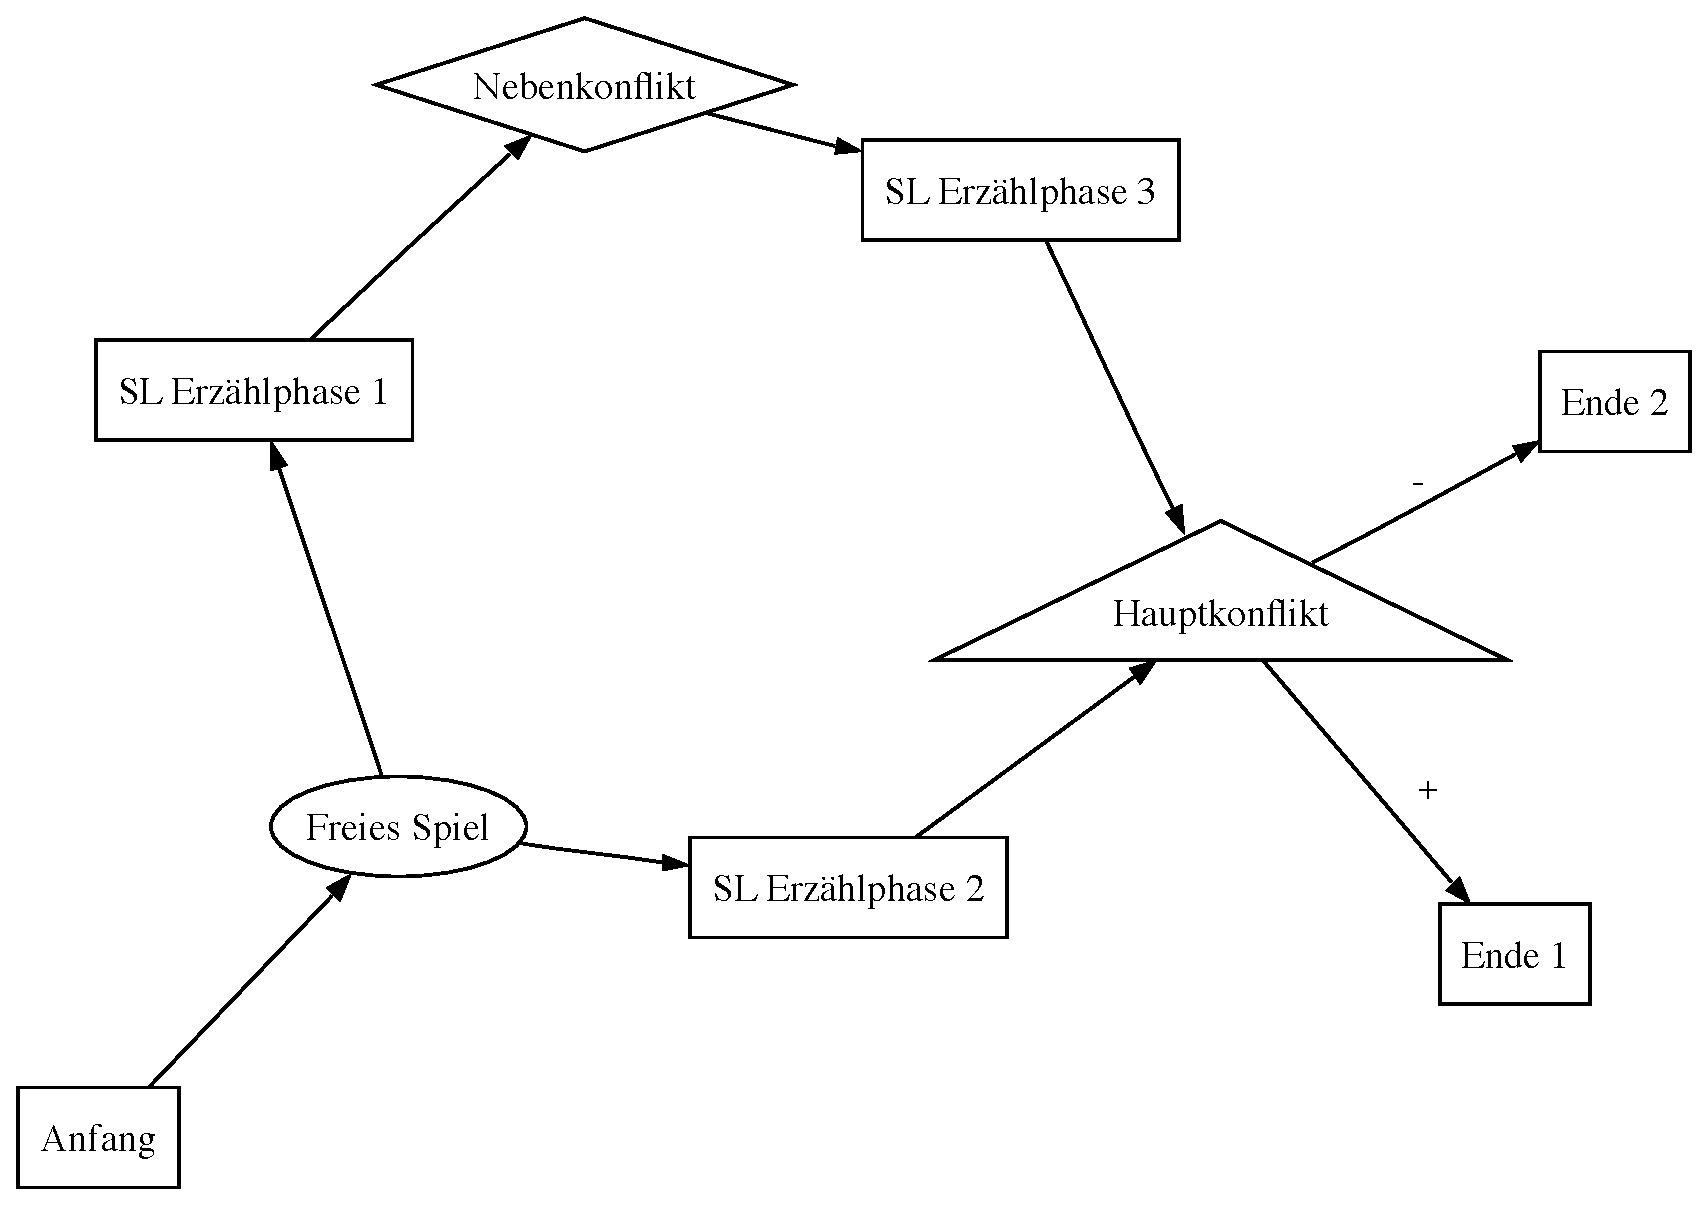
\includegraphics[width=0.95\textwidth]{pics/fluss1}}
\end{figure}

Fluss-Diagramme k"onnen auf verschiedene Arten benutzt werden: Ersten kann man mit ihnen, wie gerade angedeutet, den Verlauf des Abenteuers vorplanen. Zweitens k"onnen damit aber auch Handlungen von SLCs geplant werden. So k"onnten beispielsweise ein paar SLCs einen Einbruch geplant haben und die SCs versuchen, diesen zu entdecken. Legt der Spielleiter vorher einen Ablaufplan mit Zeiten f"ur den "Uberfall an, so kann er die Spieler im freien Spiel entscheiden lassen, wohin sie sich wann wenden wollen und dann entsprechend darauf reagieren.

\subsection{Karten}
\DEF{Karten}\index{Karte} eignen sich besonders für die Organisation von orts- und ereignisbasierten Abenteuern. Eine Landkarte, Stadtkarte oder Grundrisszeichnung hilft außerdem, sich den Ort besser vorstellen zu können. In solche Karten werden dann die Orte der Stationen und Ereignisse eingetragen.

Übergänge zwischen den einzelnen Stationen und Ereignisse werden dann im Spiel zu SL-Erzählphasen, Entscheidungen für das weitere Vorgehen werden im freien Spiel getroffen und das, was an wichtigen Dingen an den Stationen passiert, wird als Konflikte ausgetragen.

Karten sind oft nützliche Hilfsmittel, trotzdem sollte man es nicht mit ihnen übertreiben, da durch Karten auf immer eine Menge Freiheit verloren geht. So könnte die Grundrisszeichnung eines Hauses, das den Schauplatz für den großen Endkampf darstellt, die Spieler in ihren Erzählungen unnötig einschränken. Darüberhinaus ist die Erstellung einer Karte auch meist mit viel Arbeit für den Spielleiter verbunden -- und wenn eine Karte nicht unbedingt für einer orts- oder ereignisbasiertes Abenteuer benötigt wird, dann ist der Nutzen im Vergleich zum Aufwanf meist doch eher klein.

\subsection{Zeitplan}
In ereignisbasierten Abenteuern ist ein \DEF{Zeitplan}\index{Zeitplan} fast unverzichtbar und wesentlich wichtiger als eine Karte. Im Zeitplan sind alle Ereignisse aufgelistet, die vom Spielleiter vorbereitet sind. Oft hängen die Ereignisse auf gewisse Art und Weise zusammen, so dass sich bei genügend großer Komplexität für die Form des Zeitplans auch ein Flussdiagramm anbieten könnte. Der Weg durch diesen Zeitplan wird dann durch die Handlungen der Spielercharaktere festgelegt.

Im Gegensatz zum Flussdiagramm oben ist ein Zeitplan aber immer an die fortschreitende Zeit gekoppelt. Insbesondere wird man im Zeitplan üblicherweise nicht rückwärts gehen. Ausgehend von der Situation zu Beginn des Abenteuers verzweigen sich die Wege oder vereinigen sich wieder.

Aber auch für alle anderen Abenteuertypen sind Zeitpläne interessant. Es ist nützlich für den Spielleiter, eine \DEF{Eskalation}\index{Eskalation} der Situation in der Hinterhand zu haben, um die Charaktere (notfalls mit Gewalt) ins Abenteuer zu bringen. Dazu sollte der Spielleiter eine Folge von Ereignissen festlegen, die bestimmte Flaggen der Spielercharaktere und die Gefühle der Spieler (z.\,B. Hilfsbereitschaft, Kriegerehre, Moral) massiv ansprechen. Reagieren die Spieler nicht auf das Abenteuer, so kann der Spielleiter die Ereignisse der Eskalation eintreten lassen und so die Aufmerksamkeit auf das Abenteuer lenken. Der Zeitplan für eine Eskalation der Situation ist also normalerweise kein Zeitplan, der strikt eingehalten wird. Vielmehr ist es ein Notfallplan, der benutzt werden kann, um Langeweile am Spieltisch zu verhindern.




\subsection{Konfliktnetzte}
Bei einem Konfliktnetz geht es darum, Konflikte zwischen verschiedenen Gruppierungen und Charakteren graphisch übersichtlich darzustellen. Daher eignen sie sich besonders für charakterbasierte Abenteuer. Dazu werden f"ur alle beteiligten Gruppen gro"se Rechtecke auf ein Blatt gemalt, f"ur die Charaktere Ovale. Geh"ort ein bestimmter Charakter zu einer Gruppe, so werden die Charaktere in die Gruppen hineingezeichnet.

Desweiteren werden Charaktere und Gruppen untereinander mit Linien verkn"upft. Ans Ende werden Symbole gemalt, die dann f"ur eine bestimmte Grundhaltung steht. Dabei steht zur Verf"ugung:
\begin{itemize}
  \item ist freundlich gegen"uber (Kreis)
  \item ist feindlich gegen"uber (Dreieck)
  \item benutzt (Quadrat)
  \item kennt (Querstrich)
\end{itemize}

Es ist wichtig, dass im Konflikt-Netz nur Personen und Gruppen auftauchen, die f"ur die Geschichte relevant sind und auch miteinander verkn"upft sind. Es muss keine direkte Verbindung geben, jedoch sollte jeder Charakter "uber irgendwelche Wege mit jedem anderen Charakter verbunden sein. Ein Beispiel f"ur ein solches Konflikt-Netz ist auf Seite~\pageref{ConflictWeb1} zu finden.

Zusätzlich können diese Linien noch mit genaueren Informationen beschriftet werden, wie z.\,B. ``verheiratet'', ``Rivalen'', ``streiten um die Erbschaft'' usw.

\begin{figure}
\centerline{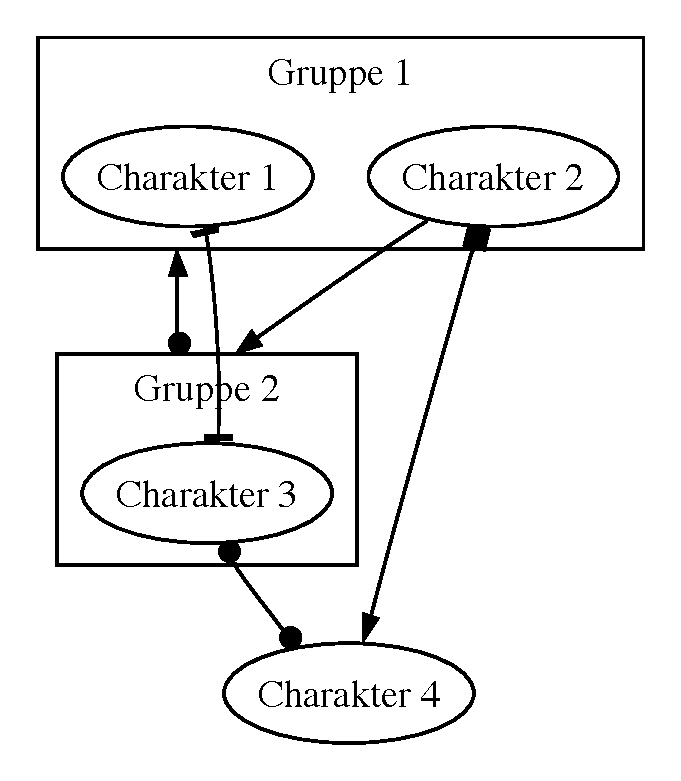
\includegraphics[height=0.55\textheight]{pics/web1}}

\paragraph{Erkl"arung des Schaubildes:} Charaktere~1 und~2 geh"oren zu Gruppe~1, Charakter~3 ist Mitglied von Gruppe~2 und Charakter~4 geh"ort keiner Gruppe an. Grunds"atzlich ist Gruppe~1 freundlich gegen"uber von Gruppe~2, Gruppe~2 aber feindlich gegen"uber Gruppe~1. Wahrscheinlich gibt Gruppe~2 vor, freundlich zu sein und Charakter~2 hat dies durchschaut, er ist n"amlich (als Ausnahme aller Charaktere aus Gruppe~1) feindlich gegen"uber Gruppe~2.

Charaktere~1 und 3 kennen sich zwar, haben aber sonst keine Meinung voneinander (d.\,h. sie wissen wahrscheinlich auch nichts von ihrer Gruppenzugeh"origkeit). Charakter~2 kann Charakter~4 nicht leiden, wird aber von diesem benutzt. Dagegen sind Charaktere~3 und 4 befreundet.

\label{ConflictWeb1}
\end{figure}








\section{Flaggen und Bangs}
Das wichtigste Hilfsmittel f"ur eine auf die Charaktere zugeschnittene Geschichte liefern die Charakterb"ogen und da insbesondere die Fragen an den Spieler und die Hintergrundgeschichte. Alles, was auf die Interessen der Spieler hindeutet, wird im folgenden als \DEF{Flagge}\index{Flagge} bezeichnet, also evtl. auch die Wahl der Profession, die Talente und die Vor- und Nachteile. Denn auch diese geben Aufschluss dar"uber, in welche Richtung die Geschichte gehen soll. So wird beispielsweise eine Gruppe Bannstrahler kaum stimmig in eine Geschichte verwickelt werden k"onnen, in der sie in einer heimlichen Nacht-und-Nebel-Aktion mit magischen Hilfsmitteln in eine Festung eindringen und einen Gegenstand stehlen m"ussen.

Das einfachste ist, dass sich der SL zun"achst einmal ein leeres Blatt nimmt und die Charakternamen weit verteilt drauf schreiben (z.\,B. einen in jede Ecke). Dann schaut er sich die Charakterb"ogen an und notiert die erkennbaren Flaggen in Stichworten in der N"ahe der Charakternamen. Sollten dem Spielleiter einzelne Flaggen nicht zusagen so kann er sie nat"urlich auch ignorieren, aber insgesamt sollten so jedem Charakter eine Handvoll Flaggen zugeordnet werden. Dieses \DEF{Flaggen-Blatt}\index{Flaggen-Blatt} sollte sich der SL dann gut sichtbar an die Seite legen, damit er immer wieder darauf zur"uckgreifen kann.

Im Laufe der Planung einer zugeschnittenen Geschichte wird immer wieder davon die Rede sein, dass die Flaggen der Charaktere angesprochen werden sollen. Das bedeutet, dass beispielsweise ein Krieger bei seiner Ehre gepackt wird, dass die Mutter eines Charakters, die die wichtigste Person darstellt, bedroht wird usw.

Dabei sollte der SL versuchen, den Charakterspielern ab und zu einen richtigen \DEF{Bang}\index{Bang} vorzuwerfen, d.\,h. eine Spielsituation, die die folgenden beiden Kriterien erf"ullt:
\begin{enumerate}
  \item Der Charakter muss zur Handlung gezwungen werden
  \item Es gibt keine richtige oder falsche L"osung
\end{enumerate}

\begin{beispiel}
  \paragraph{Drei Beispiele:}
  \begin{enumerate}
    \item Ein Unbekannter kommt zum Charakter: ``Meine Frau ist entf"uhrt! Bitte rettet sie!'' Hierbei handelt es sich nicht um einen Bang, denn a) kann der Charakter einfach sagen ``Nee, mir doch egal.'' Damit w"are er der Situation entflohen, das Spiel w"are langweilig. Die Bindung des Charakters an einen Unbekannten ist hier einfach nicht stark genung. b) W"are die richtige L"osung in diesem Fall eindeutig, die Frau zu retten.

    \item Der beste Freund des Charakters kommt: ``Meine Frau ist entf"uhrt! Bitte rettet sie!'' Das ist schon besser, denn der Charakter kann der Situation nicht entfliehen, denn schlie"slich handelt es sich um seinen besten Freund. Trotzdem ist es kein echter Bang, denn die richtige L"osung lautet immer noch, die Frau zu retten. In dieser Situation wird eine Flagge des Charakters angesprochen.

    \item Der beste Freund des Charakters kommt: ``Meine Frau ist entf"uhrt! Bitte rettet sie!'' Kurz nachdem der Freund weg ist, bekommt er eine Nachricht von der Frau, dass sie gar nicht entf"uhrt wurde, sondern geflohen ist. Sie hat ihren Mann erwischt, wie er sie betrogen hat. Daraufhin habe dieser sie eingesperrt und geschlagen. Was ist jetzt richtig? Der Frau zu glauben und sie zu unterst"utzen? Dem Freund zu helfen? Dies ist ein echter Bang.
  \end{enumerate}
\end{beispiel}

Es ist ziemlich schwierig, einen Bang zu erschaffen, der mehrere Charaktere gleichzeitig anspricht. Einfacher (aber auch noch schwierig genug) ist es, miteinander verbundene Bangs zu erschaffen. Um das zu erreichen, sollten die Flaggen der verschiedenen Charaktere bereits Ankn"upfungspunkte bieten. Dabei k"onnen die beiden Spieler "ahnliche oder entgegengesetzte Flaggen gehisst haben. Fallen dem SL solche Ankn"upfungsm"oglichkeiten auf, so kann er diese auf seinem Flaggen-Blatt durch Linien miteinander verbinden. So kann er auf einen Blick sehen, wie er eventuell mehrere Charaktere mit einer Situation ansprechen kann.

M"ochte der SL entgegengesetzte Flaggen ansprechen, so sollte dies bereits bei der Charaktererschaffung mit der gesamten Gruppe abgesprochen werden. Dann wird es n"amlich wahrscheinlich dazu kommen, dass die Spieler gegeneinander arbeiten, was nicht unbedingt von allen Spielern gew"unscht oder erwartet wird.

Nat"urlich muss auf keinen Fall jede Situation, in die die Charaktere geraten, ein Bang sein. Bangs sind das Salz in der Suppe und tragen dazu bei, dass Charaktere mehr Tiefe bekommen, da die Spieler Entscheidungen "uber die ihnen wichtigen Charakterz"uge treffen und dadurch ihren Charakter auf dieser Ebene weiter entwickeln. Daher ist es auch sinnvoll, dass der SL versucht, gleichm"a"sig f"ur alle Charaktere Bangs zu entwickeln und ins Spiel einzubringen.




\section{Aufh"anger und Ausl"oser}
Den Anfang der Planung bilden ein \DEF{Aufh"anger}\index{Aufhänger} und ein \DEF{Ausl"oser}\index{Auslöser}. Der Ausl"oser ist meist eine Person, ein Monster oder ein Ereignis und ist der eigentliche Grund f"ur das Abenteuer, ohne ihn h"atte das Abenteuer nicht stattgefunden. In vielen F"allen handelt es sich um den B"osewicht, den die Charaktere erst im Verlauf des Abenteuers aufsp"uren. Auf jeden Fall ist er der Anlass daf"ur, dass der Aufh"anger `passiert'. Der Aufh"anger ist n"amlich das, womit die Charaktere am Anfang konfrontiert werden und was sie zum Abenteuer bringt. Zu diesem Zeitpunkt muss sich der SL noch keine offensichtliche Verbindung zwischen Aufh"anger und Ausl"oser "uberlegt haben; das wird sich im weiteren Verlauf dann zeigen.

Als Ideenschmiede sind in der Tabelle auf Seite~\pageref{AufhaengerUndAusloeser} ein paar Aufh"anger und Ausl"oser zusammengetragen; soll eine zuf"allige Geschichte erzeugt werden, k"onnen beide Komponenten auch ausgew"urfelt werden. Wichtig dabei ist, dass diese Aufz"ahlung auf keinen Fall vollst"andig ist. Au"serdem ist es g"unstig, besonders bei dem Aufh"anger einen oder mehrere Flaggen der Charaktere anzusprechen, d.\,h. auch W"urfelergebnisse sollten daraufhin "uberpr"uft werden, ob das Ergebnis zu den Charakteren passt.

Teilweise k"onnen auch Aufh"anger als Ausl"oser benutzt werden: So k"onnen ein Mord, eine Verwechselung oder ein magisches Artefakt problemlos als Ausl"oser benutzt werden. 

Die etwas uneindeutige Formulierung in der Tabelle ist im "Ubrigen Absicht. Die genauen Details m"ussen nat"urlich ausgearbeitet werden. Es kann sein, dass der Spielleiter schon jetzt eine Idee hat, was sich hinter den Begriffen verbirgt, es kann aber genauso sein, dass er noch keine Ahnung hat.

\begin{table}[t]
\begin{tabular}[C]{cl@{\qquad}l}
    & \textbf{Aufh"anger} & \textbf{Ausl"oser} \\
  1 & tote Tiere & ehemaliger Mitarbeiter \\
  2 & Diebesgut & Dieb/R"auber \\
  3 & "Uberfall & Meckerdrachen \\
  4 & unschuldiges Opfer & Feenwesen \\
  5 & Mord & H"andler \\
  6 & Verwechselung & Orkbande\\
  7 & Person auf der Flucht & Paktierer\\
  8 & Auftrag & Monsterhorde \\
  9 & Albtr"aume & politischer Gegner \\
 10 & Illusionsmagie & Handwerker \\
 11 & Landkarte & Adliger \\
 12 & Unfall & bekannte Pers"onlichkeit \\
 13 & Gefangennahme & KGIA \\
 14 & Aufstand & Geist/Untoter \\
 15 & Wettbewerb & Spion \\
 16 & Sklavenhandel & Drachen \\
 17 & Krieg & Magier \\
 18 & Artefakt & Krieger/Ritter \\
 19 & verlassenes Dorf & Geweihter \\
 20 & Naturgewalt & Dienstleister \\
\end{tabular}
\label{AufhaengerUndAusloeser}

\medskip\hrule
\end{table}

Damit beginnt man mit mit der Planung an beiden Enden gleichzeitig: Einerseits mit dem Anfang der Geschichte, andererseits mit dem Ende, dem Hintergrund. Im weiteren Verlauf der Abenteuer-Planung geht es darum, beide Enden miteinander zu verbinden. Was Anfangs vielleicht widersprüchlich scheint, fügt sich hinterher meist zu einer interessanten Geschichte. Sollten einmal Aufhänger und Auslöser nicht zusammen passen, so ist es natürlich kein Problem, auch nachträglich noch (evtl. sogar im laufenden Spiel) Aufhänger und/oder Auslöser an die gegebene Geschichte anzupassen.


\section{Weitere Beteiligte im Konflikt-Netz}
Au"ser dem Ausl"oser und den Charakteren haben die meisten Geschichten noch weitere wichtige Charaktere oder Gruppen. Daher werden jetzt zun"achst in einem zweiten Schritt noch ein paar weitere SLCs ausgew"ahlt. Ideen finden sich in der Aufh"anger/Ausl"oser-Liste und k"onnen auch aus den bereits gew"ahlten Elementen ergeben.

Der folgende Vorschlag beruht darauf, dass der Spielleiter zunächst die wichtigen Spielleitercharaktere für sein Szenario erschaffen will. Das bedeutet umgekehrt, die hier vorgestellte Methode eignet sich nicht dazu, rein dingliche Abenteuer vorzubereiten oder solche, bei denen SLCs nur eine sehr untergeordnete Rolle spielen.

Für Charaktere und deren Beziehung untereinander eignet sich der Entwurf eines Konfliktnetzes für das Abenteuer. Beim Entwurf solchen Netzes oder eines Abenteuers auf eine andere Art sollte die erste Regel des Abenteuer-Entwurfs niemals aus den Augen gelassen werden: \emph{Mache das Abenteuer nicht kompliziert, denn das besorgen die Spieler schon von ganz alleine.} Das Offensichtliche ist meist besser, als man denkt, denn was für einen selbst offensichtlich ist, das ist für andere Leute meist überraschend. Viele Spielleiter und Autoren übertreiben es und verheddern sich in Kleinigkeiten, die während des Spiels dann doch übergangen oder ausgelassen werden, da sie keiner mehr versteht.

Daher sollten keinesfalls insgesamt mehr als vier weitere Gruppen (zusätzlich zu den Helden) an der Geschichte beteiligt sein. Die magische Zahl hierbei lautet drei: Drei Gruppen sind nicht zu unübersichtlich und eröffnen vielfältige Optionen. Das ergibt dann etwa drei bis sechs wichtige SLCs, eventuell bis zu zehn. Dabei sollte aus jeder beteiligten Gruppe mindestens ein, möglichst zwei konkreter SLC ausgew"ahlt werden.

Diese Charaktere werden in einem Konflikt-Netz angeordnet. 
Aber wie baut man jetzt ein solches Netz auf? Ein guter Ausgangspunkt sind drei Parteien (f"ur ein kurzes Szenario auch zwei), zunächst ganz ohne spezielle Charaktere. Zwei dieser Parteien sollten auf jeden Fall im Streit liegen. Die dritte Partei k"onnte weitere eigene Ziele verfolgen, die den anderen beiden schaden, vielleicht auch den beiden anderen "ubergeordnet sein oder noch anders. Außerdem sollte der Ausl"oser jetzt schon ins Netz eingebaut werden: Als Mitglied einer der Parteien oder auch als eigenst"andiger Charakter. Im letzteren Fall sollte dieser auf jeden Fall mit zwei der bestehenden Parteien verkn"upft werden (evtl. auch nur mit einer, das vereinfacht das Szenario nochmals).

Im zweiten Schritt sollte sich herauskristallisieren, wie Ausl"oser und Aufh"anger zusammenh"angen und um was es "uberhaupt geht. Dazu braucht man noch ein paar Charaktere, die die Gruppen repr"asentieren. Als Faustregel gilt, dass in einer Gruppe nicht mehr als drei Charaktere auftauchen sollten, denn es sollen ja nur die wichtigen Charaktere aufgef"uhrt werden. Zu gro"se Netze sind zu verwirrend und f"uhren dazu, dass der Wiedererkennungseffekt einzelner Personen und Gruppen klein ist. Ein bis zwei wichtige Charaktere pro Gruppe sollte es aber schon sein. Dazu noch eventuell ein paar au"senstehende Charaktere. Die Charaktere brauchen noch keine Namen oder Bedeutungen, erstmal einfach nur Ovale.

Die neu eingef"uhrten Charaktere werden auch wieder mit Verbindungslinien in das Konflikt-Netz eingef"ugt und mit Dreiecken, Kreisen, Quadraten und Querstrichen versehen. Dabei sind zus"atzliche Konflikte und Beziehungen innerhalb einer Gruppe genauso interessant wie pers"onliche Beziehungen "uber Gruppen hinweg oder auch besondere Sichtweisen einer Person zu einer anderen Gruppe.

Bei der Erg"anzung der Linien und Symbole sollten die Gruppen benannt werden und die einzelnen Charaktere eine Grundmotivation erhalten, wodurch dann auch die Symbole erkl"art werden. Am Ende sollte ein Netz entstanden sein, dass recht komliziert (aber nicht zu verwirrend) ist. Dar"uberhinaus sollte klar sein, wie die Charaktere zusammenh"angen und was ihre Grundmotivation ist. Insgesamt solllte eine konfliktreiche Situation entstanden sein, in der es geh"orig kracht, wenn niemand eingreift.

Die Erstellung des Konflikt-Netzes und das Hinzunehmen weiterer Beteiligter ist nicht streng getrennt sondern ein sich gegenseitig beeinflussender Prozess, in den auch immer wieder die Flaggen der Spieler mit einbezogen werden. Au"serdem sollte f"ur jeden SLC sofort notiert werden, welche Flagge welches Charakters diese ansprechen sollen. Das kann auch gemacht werden, indem auch die SCs mit ihren Flaggen im Konfliktnetz eingebunden werden. Spricht ein SLC eine Flagge an, so wird eine gestrichelte Linie vom SLC zur Flagge gezeichnet.




\section{Beziehung zu den SCs}
Darüberhinaus müssen die Charaktere mit ins Spiel kommen und mit den SLCs in Verbindung gebracht werden. Je nach Einstellung k"onnen die SLCs im Konflikt-Netz farbig markiert werden. Es gibt folgende Grundeinstellungen der SLCs gegen"uber der Charaktere:
\begin{itemize}
  \item Der SLC will den SCs helfen (gr"un)
  \item Der SLC will Hilfe von den SCs (blau)
  \item Der SLC m"ochte die SCs missbrauchen (gelb)
  \item Der SLC ist ein offener Gegner der SCs (rot)
\end{itemize}

Fast unabh"angig von ihren Motivationen und Beziehung zu den SCs kann der Spielleiter den SLCs nun einen oder mehrere der folgenden Charakterz"uge zuordnen:
\begin{itemize}
  \item verzweifelt
  \item "Uberrekation
  \item brutal
  \item verantwortungslos
  \item unmoralisch
  \item irrational/fanatisch
  \item verheimlichen
  \item neidisch/eifers"uchtig
\end{itemize}
Diese Charakterzüge beschreiben die Charaktere, wenn sie bedrängt sind und sehen, dass ihre Ziele in weite Ferne rückt.

Sp"atestens jetzt sollte klar sein, welche SLCs welche Flaggen der SCs ansprechen. Es sollte m"oglichst kein SLC ohne Flagge mehr sein; umgekehrt sollten auch von allen SCs Flaggen angesprochen werden. Nat"urlich sollen in einer Story nicht nur aus Charakteren bestehen, die direkt Flaggen ansprechen; jedoch handelt es sich bei den Charakreren des Konflikt-Netzes um die Hauptfiguren, mit denen die Spieler sehr oft zu tun haben werden.

Dazu ist es noch sinnvoll, \DEF{Handlungsgrenzen}\index{Handlungsgrenzen} festzulegen. Diese Grenzen legen fest, wie weit der SLC bereit ist zu gehen, um seine Ziele durchzusetzen. Diese Grenzen sollten flexibel gehandhabt werden und an die aktuelle Spielsituation angepasst werden; jedoch ist eine solche Handlungsgrenze eine gute Improvisationshilfe. 




\section{Kampagnen und Abenteuer}
Das jetzt fertige Konflikt-Netz soll dazu dienen, eine Grundlage f"ur den Anfang einer gesamten Kampagne zu bieten. Dabei kann der gewählte Auslöser entweder das Ende des aktuellen Abenteuers oder aber auch das Ende der gesamten Kampagne darstellen. Üblicherweise ist eine selbst gemachte Kampagne niemals eine von vorne bis hinten durchgeplante Folge von Abenteuern, sondern wird je nach Lust und Laune an die Spielsituation angepasst. Genauso flexibel muss der Spielleiter dann auch mit dem Konfliktnetz umgehen, es immer wieder anpassen, neue Gruppierungen und Charaktere hinzunehmen und alte, verbrauchte oder uninteressante SLCs entfernen. Dabei sollte die Gesamtgröße immer in etwa gleich bleiben.

Am Ende einer Kampagne entscheiden dann die Spieler gemeinsam, ob sie mit den gleichen Charakteren eine weitere Kampagne spielen wollen, oder ob sie lieber eine neue Kampagne mit neuen Charakteren beginnen wollen. Spätestens jedoch wenn die Charaktere Stufe 21 erreichen ist das Abenteuerleben beendet.

Während des Verlaufs einer Kampagne oder einer Folge von Kampagnen muss der Spielleiter auch immer die Bedeutung der momentanen Stufe der Helden im Hinterkopf haben. Sind die Herausforderungen und Geschichten am Anfang noch lokaler Natur und stolpern die Helden mehr oder weniger zufällig in die Abenteuer, so kommen doch relativ bald (ab Stufe 6) Auftraggeber auf sie zu. Zunächst noch aus der direkten Umgebung, später dann (ab Stufe 12) auch aus weiter entfernten Gegenden. Spätestens ab Stufe 18 betreffen die Abenteuer die Geschicke von Ländern. Die Charaktere führen Heere, bekämpfen Drachen und sind im höheren Adel als Streiter für die gerechte Sache bekannt.





\section{Planung der Abenteuer}
Im Normalfall k"onnen sich mehrere Abenteuer aus einem einzigen Konflikt-Netz ergeben. Es steckt voller Konflikte, hat aber bereits einen Anfang: den Ausl"oser. Ausgehend von dem Ausl"oser sollte der Spielleiter leicht ein Abenteuer-Szenario erschaffen k"onnen. Je nachdem, ob die Kampagne nur aus einem oder aus mehreren Abenteuern bestehen soll, sollte der Spielleiter mehr oder weniger vom Konflikt-Netz f"ur das Abenteuer verwenden.

Oft ist es günstig, wenn ein Abenteuer dem Aufbau eines klassischen Dramas folgt. Das gibt eine klare Struktur:
\begin{enumerate}
  \item Einleitung (Exposition)
  \item Mittelteil (Konfrontation)
  \item Ende (Katastrophe/L"osung)
\end{enumerate}
Ob ein Abenteuer dieser Struktur folgt oder nicht ist zwar den meisten Spieler im Prinzip egal, jedoch erleichtert sie dem Spielleiter die Festlegungs des Tempos, mit dem er im Abenteuer vorgeht (`Pacing'). Zudem ist es für die Spieler befriedigend, wenn sie nach einer klaren Katastrophe oder der eindeutigen Lösung wissen, dass sie ein Abenteuer erfolgreich abgeschlossen haben (oder eben nicht).

Die \DEF{Einleitung}\index{Einleitung} soll die Spieler in die Geschichte, in die Stimmung und die Situation einf"uhren. Im diesem ersten Teil sollten die wichtigen Personen eingef"uhrt werden, die in dem Abenteuer eine Rolle spielen. Auch sollte sich hier ein vordergr"undiges Ziel der Charaktere herauskristallisieren. Szenen der Einleitung umfassen typischerweise Einf"uhrung von neuen Fakten (z.\,B. neue Spielleiter-Charakter, Ereignisse) und erweitern damit das Wissen der Charaktere und Spieler. Dar"uberhinaus bildet die vermittelte Stimmung die Grundlage f"ur das Abenteuer.

Der \DEF{Mittelteil}\index{Mittelteil} ist der Hauptteil des Abenteuers und kann recht umfangreich sein. Die Charaktere arbeiten auf ihr Ziel hin. Dabei kann es dazu kommen, dass sie zun"achst weitere Handlungsstr"ange aufdecken. Am Ende des Mittelteils werden die jedoch wieder auf die wesentlichen Str"ange reduziert sein, so dass das Abenteuer dann seinen Abschluss finden kann.

Der Mittelteil l"asst sich oft nochmals zweiteilen. Nach der Einleitung steigert sich die Spannung, indem sich die ganze Sache verkompliziert, neue Optionen offen stehen und Pl"ane geschmiedet werden. Das sind die bereits erw"ahnten Handlungsstr"ange, die aufgedeckt werden. Der Spannungsh"ohenflug endet dann mit der Reduktion von Str"angen, indem die SCs dann Fehlschl"age erleben, einer falschen Spur nachgehen o.\,"a. Nach einer Neuorientierung folgen dann die SCs den richtigen Handlungsstr"angen hin zum Ende. Ein nur einteiliges Mittelst"uck dagegen steigert die Spannung bis zum Ende. Diese Art von Abenteuern sind aber naturgegeben wesentlich k"urzer, da sich die Spannung nat"urlich nicht bis ins unendliche steigern kann.

Das \DEF{Ende}\index{Ende} des Abenteuers f"uhrt schlie"slich die meisten der noch offenen Handlungsstr"ange zusammen. Die Probleme k"onnen sich aufl"osen oder auch nicht. In jedem Fall ist die Handlung abgeschlossen, das Ziel der Charaktere ist entweder entg"ultig erreicht oder entg"ultig verfehlt. Ist das Abenteuer nicht gleichzeitig der Abschluss der Kampagne, so l"auft diese noch weiter. In diesem Fall bleiben noch einige Handlungsf"aden offen und einige Fragen ungekl"art, was dann als Anschluss f"ur ein n"achstes Abenteuer dient. Im Gegensatz dazu bedeutet das letzte Ende einer Kampagne auch (zun"achst) den Abschluss der gesamten Handlung der Charaktere. Nach einem Kampagnenende sollte keine Frage mehr offen sein, alle Handlungsstr"ange werden abgeschlossen.

\section{Zwischen den Abenteuern}

Neuer Ausl"oser

K"urzen des Konflikt-Netzes (abgearbeitete SLCs rausnehmen)

Erweitern des Konflikt-Netzes (evtl. neue SLCs hinein, neue Verbindungen nach der Geschichte, usw.)


\section{Beispiel f"ur eine zugeschnittene Geschichte}
Das folgende Beispiel ist die Grundlage f"ur das Einsteiger-Abenteuer-Szenario. Spieler, die das vielleicht noch spielen wollen, sollten daher dieses Beispiel einfach "uberspringen.



\subsection{Die Charaktere}
In diesem Beispiel soll eine Kampagne f"ur die Charaktere aus dem Beispiel ab Seite~\pageref{BeispielCharaktere} entstehen.



\subsection{Flaggen und Bangs}
Folgende Flaggen k"onnte ein Spielleiter aus den Fragen an den Spieler ausmachen:
\begin{description}
  \item[Tharam] Duell, Rondra-Glaube und Ehre, Mutter, Ehrlichkeit, Ziliane
  \item[Ziliane] Verhandlungen, Diebereien, Abenteurer-Gruppe, L"ugen
  \item[Bodowius] Mysterien/Magie, gro"se Liebe, Pazifismus, schwarze Magie
  \item[Denidara] Elfin, liebt Natur/f"urchtet St"adte, Selbstlosigkeit
\end{description}

F"ur Bangs eignen sich "ublicherweise Kombinationen aus einer Personen, die die Charaktere sehr sch"atzen und Handlungen dieser, die den Leidenschaften entgegensteht. Eine andere M"oglichkeit ist, dass zwei wichtige Bekannte gegeneinander arbeiten und ein Charakter muss sich f"ur eine Seite entscheiden.

Bei diesen Charakteren gibt es unter anderem folgende M"oglichkeiten:
\begin{enumerate}
  \item Tharam: Rondra-Ehre gegen Mutter
  \item Tharam: Ziliane gegen Rondra-Ehre/Ehrlichkeit oder gegen Mutter (Vorsicht bei Konflikten innerhalb der Gruppe!)
  \item Bodowius: Pazifismus gegen gro"se Liebe
  \item Denidara: Selbstlosigkeit gegen ihre Liebe zur Natur
\end{enumerate}
F"ur Ziliane ist es schwierig, zu diesem Zeitpunkt einen Bang zu finden. Schwierig deshalb, weil ihre Spielerin au"ser der Gruppe und Ziliane selbst keine Personen angegeben hat, d.\,h. m"ogliche Bangs w"urden praktisch immer die Gruppe selbst betreffen.

Allerdings ist es auch nicht schlimm, wenn sich jetzt noch kein Bang f"ur Ziliane herauskristallisiert. Im Laufe des Spieles werden sich Beziehungen zu anderen SLCs ergeben, aus denen man dann sicherlich einen Bang konstruieren kann. Dar"uberhinaus f"uhren zu viele Bangs gleichzeitig dazu, dass das Spiel leicht un"ubersichtlich wird.



\subsection{Aufh"anger und Ausl"oser}
Als erstes steht die Wahl von Aufh"anger und Ausl"oser an. Ein ideenloser Spielleiter w"urfelt einfach mal 2W20: 7, 10. Das ergibt als Aufh"anger eine Person auf der Flucht und einen Handwerker als Ausl"oser. Das Spiel beginnt also mit einer fl"uchtenden Person, dahinter steckt letztendlich ein Handwerker. Letzteres klingt erstmal nicht sehr spannend; mal sehen, was sich draus machen l"asst.

\subsection{Weitere Beteiligte im Konflikt-Netz}
Der Empfehlung folgend, kommen ersteinmal drei Gruppen in das Konflikt-Netz. Wenn der Hintermann ein Handwerker ist, so k"onnte die erste Gruppe die Handwerkergilde sein, der dieser Handwerker vorsteht. Dann passt dazu noch eine `verfeindete' Gilde, vielleicht eine H"andlergilde. Da in den Vorgeschichten Donnerbach erw"ahnt wurd, die Charaktere aber auf Abenteuer ausgezogen sind, passt vielleicht Trallop und Umgebung als Kampagnen-Ort ganz gut. Also, schnell mal bei Trallop nachgeschaut: Ja, es gibt beispielsweise eine \textbf{Gilde der Schmiede} und eine \textbf{Gilde der Flussh"andler}. Die streiten sich um Geld und Macht: Vielleicht, haben die H"andler bei den Zwergen aus dem Finsterkamm eine g"unstige und qualitativ hochwertige Quelle f"ur Schmiedegut aufgetan und graben damit den Schmieden das Wasser ab. Keiner will mehr das Zeug von denen kaufen. Die Schmiede wiederum "argern sich, wie man denn mit den Finsterzwergen "uberhaupt Gesch"afte machen kann und sehen mit dem sinkenden Umsatz ihren Einfluss in der Stadt sinken.

Hm, Weiden ist dicht an den Orklanden und hat auch immer wieder mit denen zu k"ampfen. Wie w"are es also mit einem \textbf{Tordochai-Clan} als dritte Partei. Vielleicht angeheuert von den Schmieden, um den Flussh"andlern eins auf den Deckel zu geben.

Damit sind schon drei Parteien auf dem Plan: Die Schmiedegilde und die Flussh"andlergilde sind verfeindet. Die Schmiedegilde benutzt die Orks. Die Orks wiederum sind deswegen mit der Flussh"andlergilde verfeindet, denn die Orks m"ogen die Schmiede.

So, nun kommt ein paar erste Ideen f"ur SLCs: Den \textbf{Anf"uhrer der Schmiede} hatten wir ja schon, das ist der Ausl"oser; der hat auch die Orks angeworben. Als Gegengewicht zu den Orks k"onnte es auf der Seite der Flussh"andler einen \textbf{Schwarzmagier} geben. Das spricht auch sch"on Bodowius an. Au"serdem, wenn der widernat"urliche Magie praktiziert, dann macht das auch Denidara an.

Der Aufh"anger k"onnt ein \textbf{Aussteiger auf Seiten der Schmiede} wegen der Ork-Geschichte sein. Auf den hat der Ober-Schmied einen der Orks mit seiner Bande gehetzt. Das spricht wieder Bodowius an, aber auch Tharam sollte bei einem hinterh"altigen Angriff bei seiner Ehere gepackt werden und auch Denidaras Selbstlosigkeit m"usste dann klingeln.

Der Schwarzmagier nun ist von einem \textbf{Flussh"andler} angeheuert worden, der mit dem Aussteiger befreundet ist. Die Flussh"andlergilge wei"s gar nichts von dem Magier, allerdings war der entsprechende Flussh"andler durch seinen Freund immer gut informiert und konnte so dem Magier gezielt Auftr"age erteilen. Er erhofft sich damit, in der Flussh"andergilde weiter nach oben zu kommen. An der Spitze dieser Gilde steht n"amlich ein \textbf{reicher Schn"osel}, der sich anscheinend um nichts mehr k"ummert, als um seinen pers"onlichen Vorteil. Bei ihm ist sicher f"ur Ziliane was zu holen.

Auf Seiten der Orks gibt es den \textbf{Bandenf"uhrer}, der auch den Angriff auf den Aussteiger organisiert. Heimliches und tats"achlich geisiges Oberhaupt des Clans ist jedoch der \textbf{Ork-Schamane}. Die Tordochai halten sich im "ubrigen im Finsterkamm auf, im faktischen Niemandsland zwischen Weiden und dem Orkland. Da es keine gr"o"seren "Ubergriffe des Clans auf weidener Siedlungen gegeben hat, sind sie bislang niemandem ernsthaft aufgefallen.

Letztendlich passt nun auch ein Bang perfekt ins Geschehen: \textbf{Tharams Mutter}, die mit dem Gildenoberhaupt der Schmiede gut befreundet ist, hat ihre Stellung ausgenutzt und den Kontakt zu den Orks hergestellt. Das wird sie nat"urlich nicht so ohne weiteres zugeben wollen.

Ein anderer gut passender Bang w"are, dass der Schwarzmagier Bodowuis eine M"oglichkeit zur Heilung seiner Geliebten bietet, daf"ur aber irgendwas verlangt, was gegen er Pazifismus bzw. gegen die Anti-Schwarzmagische Einstellung Bodowius spricht.

\begin{figure}[t]
\centerline{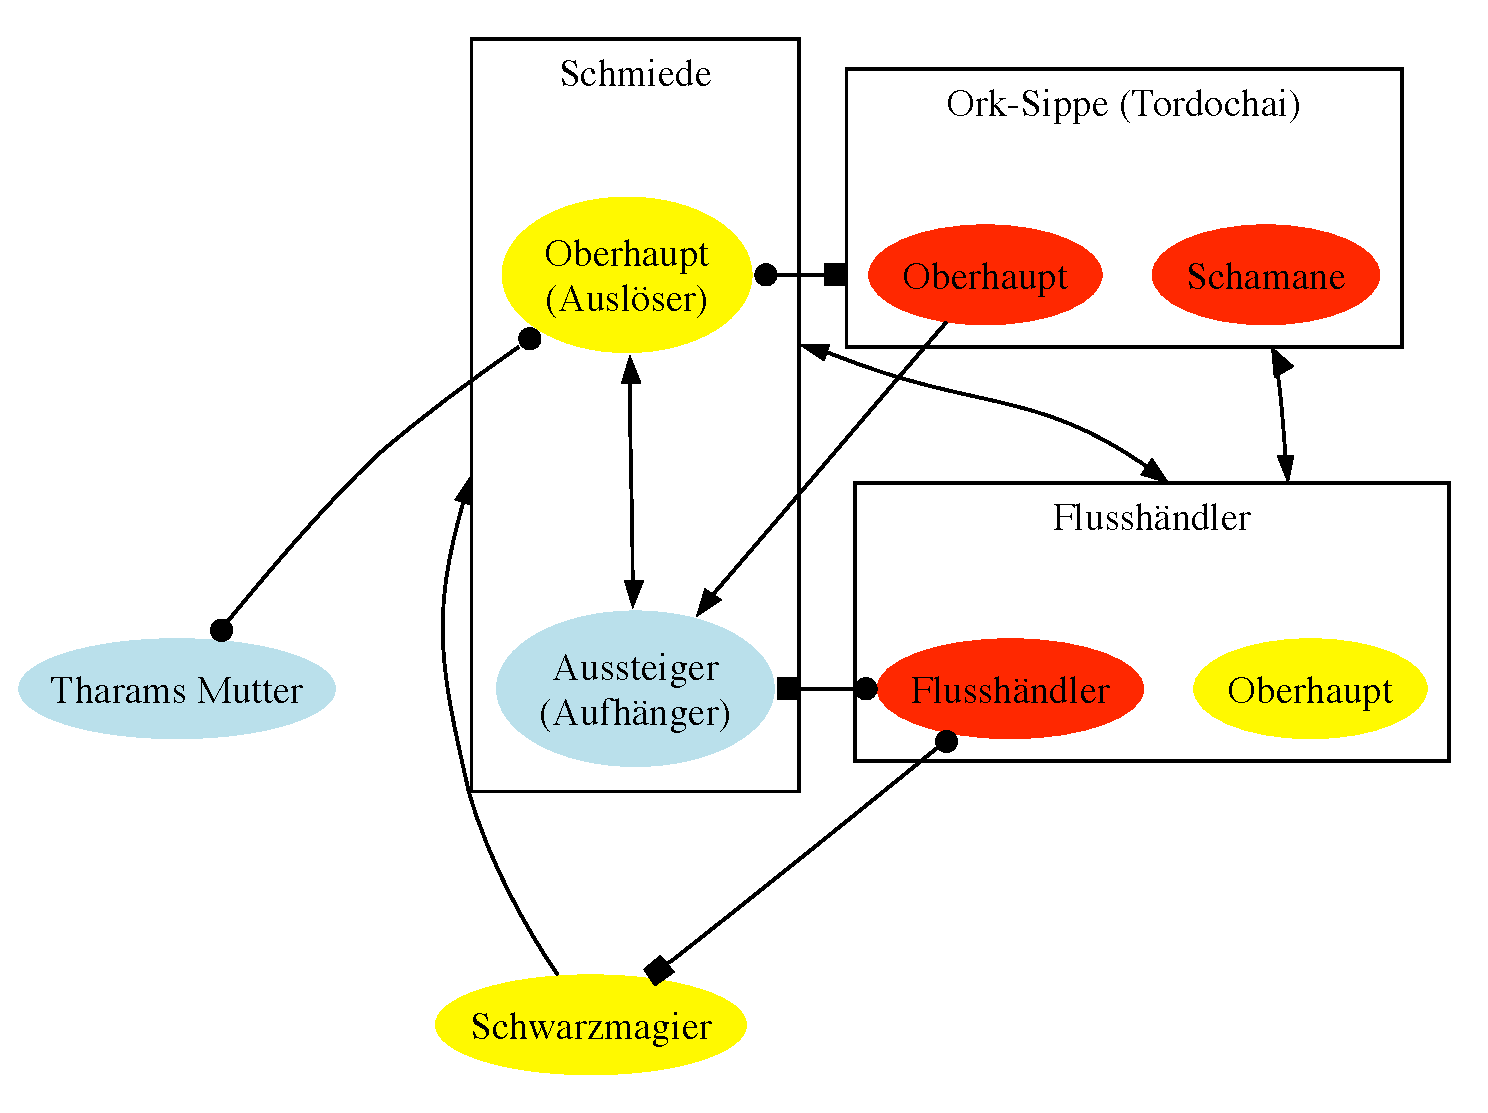
\includegraphics[width=0.95\textwidth]{pics/web2}}
\label{ABBKonfliktNetzBeispiel}
\hrule
\end{figure}

Insgesamt etwas lose angebunden ist vielleicht noch Ziliane. Jedoch durch ihre enge Anbindung an die Gruppe (immerhin die zweitwichtigste Person) und viele M"oglichkeiten zu Verhandlungen kann dieser Eindruck aber t"auschen.



\subsection{Beziehung zu den SCs}
In diesem Schritt werden die SLCs weiter ausgearbeitet. F"ur jeden SLC wird eine Motivation bzw. ein pers"onliches Ziel festgelegt und es wird gesagt, wie der SLC diese Ziele durchsetzen will, wenn die SCs auftreten: Versucht er ihre Hilfe in Anspruch zu nehmen, will er seine Ziele gegen die SCs durchsetzen oder versucht er, sie f"ur seine Zwecke auszunutzen?

Dazu werden dann noch Charakterz"uge festgelgt und sogenannte Handlungsgrenzen: Wie weit geht der SLC? Ist er eher vorsichtig oder geht er "uber Leichen? Als letztes werden noch die Flaggen notiert, die der SLC anspricht. Damit kann dann der SL die Geschichte so steuern, dass alle SCs gleicherma"sen angesprochen werden.

\begin{description}
  \item[Oberster Schmied:] M"ochte die eigene Macht st"arken und gleichzeitig den Handel zwischen Flussh"andlern und Finsterzwergen bek"ampfen. Hat R"uckhalt in seiner Gilde, dieser schwindet jedoch. Hat den Schwarzmagier bemerkt, wei"s aber nicht genau, von wem der kommt. Will SCs ausnutzen. Ist neidisch und reagiert leicht "uber. Geht im Extremfall "uber Leichen und bezahlt die Orks auch daf"ur.

  Flaggen: Ehrlichkeit von Tharam, Pazifismus von Bodowius, Selbstlosigkeit von Denidara

  \item[Aussteiger:] M"ochte Mord und Todschlag verhindern. Sucht Hilfe bei den SCs. Ist verzweifelt. Greift im Extremfall den Obersten Schmied offen verzweifelt an, um Tote durch die Orks zu verhindern.

  Flaggen: Pazifismus von Bodowius, Selbstlosigkeit von Denidara

  \item[Oberster Flussh"andler:] M"ochte seine Stellung ausbauen und beweisen, dass hinter den Orks die Schmiede stecken. M"ochte die SCs benutzen. Unmoralisch. Er ist bereit, gro"se Mengen Geld zu zahlen, um seine Ziele durchzusetzen.

  Flaggen: Ziliane Verhandlung und Klauen

  \item[Flussh"andler:] M"ochte den obersten Flussh"andler absetzen und selber an die Spitze. Nutzt den Aussteiger und den Schwarzmagier, um seine Position zu st"arken. Sieht in den SCs Feinde, die seinen Aufstieg verhindern k"onnten. Verheimlicht den Schwarzmagier und ist neidisch auf den obersten Flussh"andler. W"urde auch den Schwarzmagier gegen den obersten Flussh"andler oder seinen Schmiede-`Freund' einsetzen. Bei den SCs appelliert er an ihren Gerechtigkeitssinn.

  Flaggen: Selbstlosigkeit von Denidara

  \item[Ork-Bandenf"uhrer:] Wird durch das Geld der Schmiede motiviert. Gegner der SCs. F"uhrt brutal und fanatisch die Befehle vom obersten Schmied aus. F"uhlt sich "uberlegen und w"urde sich auch auf ein Duell mit Bodowius einlassen.

  Flaggen: Tharam Duell, Bodowius Pazifismus, Denidara Elfin

  \item[Ork-Schamane:] Sieht die Chance gekommen, dass er den Clan durch Spionaget"atigkeiten und Schl"age gegen Weiden unter den Orks nach vorne bringt. Gegner der SCs. Skrupellos, aber "uberlegt. Erkennt die SCs schnell als gef"ahrliche Gegner und geht gegen sie vor, kann sich aber nicht als Anf"uhrer aufspielen.

  Flaggen: 

  \item[Schwarzmagier:] Sieht seine Chance gekommen, "uber die H"andler die Politik von Trallop zu infiltrieren. Er nimmt den Flussh"andlern nicht wirklich ernst. M"ochte die SCs benutzen und macht daf"ur den SCs Angebote "uber magische Gegenst"ande. Er ist unmoralisch und verheimlicht den SCs gegen"uber die Verbindung zu den Flussh"andlern.

  Flaggen: Ziliane Verhandlungen, Bodowius schwarze Magie

  \item[Tharams Mutter:] Ist selber ungl"ucklich, dass sie ihre Stellung so ausgenutzt hat. Sie m"ochte die Situation aber nicht noch schlechter machen, daher versucht sie, ihren Missgriff zu verheimlichen. Wenn sie von selbst auf die Charaktere zugeht, dann braucht sie Hilfe, da ihre Verfehlung kurz vor der Aufdeckung steht.

  Flaggen: Tharam Bang
\end{description}



\subsection{Das Abenteuer}
Alleine aufgrund dieses Konflikt-Netzes kann sicherlich ein umfangreiches Abenteuer zusammengestellt werden, dass mit dem Schmied auf der Flucht beginnt, die Charaktere dann zu den Orks f"uhrt, von da k"onnten sie die Spur zu den Schmieden verfolgen und geraten dann in den Streit zwischen Flussh"andlern und Schmieden. Das ganze m"undet dann darin, dass Tharams von der Verfehlung seiner Mutter erf"ahrt und die Spieler entscheiden m"ussen, auf welche Seite sie sich stellen. Ein solches Abenteuer w"urde sicherlich einige Spielabende in Anspruch nehmen.

Soll aber das Konflikt-Netz f"ur den Auftakt einer Kampagne dienen, so sucht der SL zun"achst ein Zwischenziel. In diesem Beispiel soll es das Aufdecken der Machenschaften des Flussh"andlers sein, der den Schwarzmagier angeheuert hat und den Ausl"oser ausnutzt. Dar"uber sollen die SCs dann tiefer in den Sumpf blicken k"onnen. Das ganze Abenteuer soll als Einsteiger-Abenteuer konzipiert werden (sowohl f"ur die Chrakterspieler als auch f"ur den Spielleiter), daher wir es eine recht geradlinige und "ubersichtliche Story geben.

Daraus ergeben sich folgende drei Akte:
\begin{enumerate}
  \item Einleitung. Beginn mit einem Knaller: Kampf gegen die Orks. Der hat zwei m"ogliche Ausg"ange: Die Charaktere schaffen es, den Aussteiger zu retten oder der Aussteiger stirbt dabei. Egal wie, die Charaktere m"ussen einen Hinweis auf das Schmiede-Oberhaupt.

  \item Mittelteil. Die Charaktere sp"uren den Oberschmied auf. Der wiederum behauptet, dass der Schwarzmagier hinter der ganzen Sache steckt; er appelliert an das gute Gewissen der Helden. "Uber diesen finden sie dann den Flussh"andler, der den Schwarzmagier beauftragt hat.

  \item Ende. Die Charaktere werden mit dem Flussh"andler konfrontiert. Dieser hetzt den Schwarzmagier auf sie und erweist sich auch selber als unerwartet schlagkr"aftig.
\end{enumerate}




\chapter{Spiel-Leiten}\label{Ch:SpielLeiten}
\lettrine{E}{in} Geheimnis oder Mysterium gibts in diesen Spielregeln nicht, daher schadet es auch nichts, wenn auch Charakterspieler dieses Kapitel lesen. Es soll dem Spielleiter die n"otigen Techniken und auch ein paar Ideen liefern, eine spannende Story zu liefern.

\section{Aufgaben des Spielleiters}
Bei StoryDSA hat der Spielleiter eine recht umfassende und wichtige Aufgabe: Er lenkt die Geschichte. Das bedeutet im Normalfall, dass sich ein Spielleiter auch außerhalb des eigentlichen Spielabends vorbereitet. Das kann er mit Hilfe von fertigen Abenteuern (z.\,B. Kaufabenteuer oder Download-Abenteuer) tun oder sich selbst was ausdenken. Ideen und Hilfen hierzu gibt das Kapitel `Abenteuer vorbereiten'.

Eine zweite wichtige Aufgabe ist, das Spiel am Laufen zu halten. Das ist, neben ein paar allgemeinen Betrachtungen, der Schwerpunkt dieses Kapitels. Insbesondere bekommt der Spielleiter hier ein paar Tipps zur Improvisation. Improvisieren muss der Spielleiter nämlich immer dann, wenn die Spieler mit ihren Helden etwas machen, was der Spielleiter nicht vorbereitet hat. Das kommt sehr häufig vor und endet leider allzuoft damit, dass der Spielleiter die Ideen der Spieler beispielsweise mit einer SL-Erzählphase abwürgen muss und diese sich dann gegängelt fühlen (obwohl dem Spielleiter das nach den \StoryDSA-Regeln natürlich zusteht).

Darüberhinaus kann zur Planung ein gewisse Zeiteinteilung wichtig sein. Der Schwerpunkt bei \StoryDSA liegt auf dem gemeinsamen Spiel, also dem Freien Spiel, Nebenkonflikten und natürlich Hauptkonflikten. Für eine Phase freies Spiel oder einen Nebenkonflikt sollte der Spielleiter daher ca. 10--20 Minuten einplanen, für einen Hauptkonflikt sogar bis zu 30~Minuten. Dagegen sollten Kurzkonflikte in etwa 5~Minuten abgehandelt sein, SL-Erzählphasen sollten etwa 2~Minuten, keinesfalls aber länger als 5~Minuten, dauern.

Dauert ein Spielabend also etwa 4~Stunden, so könnte er 2~Hauptkonflikte, 5~Nebenkonflikte, 5 Phasen mit freiem Spiel und die dazugehörigen SL-Erzählphasen unterbringen. Dafür müssen die Spieler aber in den vier Stunden intensiv spielen und sich nicht lange mit Regelfragen oder Gesprächen abseits des Spieles aufhalten. Je nachdem, wie viele solche Unterbrechungen ein Spiel hat, sind es entsprechend weniger Phasen, die in 4~Stunden geschafft werden.

Die angegebenen Zeiten sind natürlich nur Richtlinien und keine Gesetze. Gerade das Freie Spiel ist in manchen Spielgruppen beliebter als in anderen. Hier sollte der Spielleiter das Spiel so lange laufen lassen, wie es allen Beteiligten Spaß macht. Sobald es anfängt abzuflauen, ist der richtige Zeitpunkt, das Spiel zu unterbrechen und mit einer Erzählphase zu einem Konflikt überzuleiten.


\section{Die Regeln}
Die erz"ahlte Geschichte ist das wichtigste Element in \StoryDSA; es geht darum, dass die Spieler eine interessante Geschichte erleben und diese in einem gewissen Rahmen selber mitgestalten k"onnen. Dazu stellen die Regeln Hilfsmittel zur Verf"ugung: Konflikte, Freies Spiel und SL-Erz"ahlphasen, die ja bereits beschrieben wurden.

Dabei sind die Regeln so angelegt, dass die Charakterspieler im wesentlichen \DEF{Richtungsentscheidungen}\index{Richtungsentscheidungen} und \DEF{Farbe}\index{Farbe} hinzuf"ugen k"onnen. Dabei bedeutet Farbe, dass die genaue Ausgestaltung zwar in der Hand der Spieler liegt, die Ereignisse selbst jedoch in der Hand des Spielleiters liegen. Farbe kommt beispielsweise bei Nebenkonflikten ins Spiel, bei denen der Spielleiter bestimmt, um was es geht, die Charakterspieler jedoch sagen, wie sie ihr Ziel erreichen. Dabei ist die Konfliktende-Regel ganz wichtig, denn kein Spieler darf das Ende vorwegnehmen.

Richtungsentscheidungen k"onnen die Spieler, wenn der Spielleiter es zul"asst, im freien Spiel treffen: Welchem Teil der Geschichte folgen die Charaktere als n"achstes, d.\,h. welcher Handlungsstrang soll weiter verfolgt werden? Ob er Richtungsentscheidungen zulassen m"ochte, sollte er den Spielern in der vorangehenden SL-Erz"ahlphase klar machen, indem er beispielsweise sagt: ``\dots und so sitzt ihr im `Goldenen Krug' und diskutiert "uber die Frage, wie es nun weitergehen soll. Was wollt ihr also tun?''

Dar"uberhinaus k"onnen Hauptkonflikte Wendungen ins Spiel bringen. Bei Nebenkonflikten steht das Ergebnis ja im Wesentlichen fest, so dass auch ein misslungener Nebenkonflikt den erw"unschten Ausgang hat; eventuell mit unerwarteten Nebenwirkungen, jedoch wird das Ziel der Charaktere erreicht. Bei Hauptkonflikten dagegen ist das Ende unklar. Das auch ein Punkt, den der Spielleiter nicht aus dem Auge verlieren darf: Wie geht es weiter, wenn die Charaktere gewinnen? Wie geht es weiter wenn die Charaktere verlieren?

\section{Charaktergeschichten und Geschichtscharaktere}
Es gibt f"ur DSA eine ziemlich gro"se Anzahl an Abenteuern, die sich f"ur \StoryDSA gut eignen, denn die meisten Autoren gehen davon aus, dass der Spielleiter die Story lenkt. So ist es meist problemlos m"oglich, Kauf- oder Downloadabenteuer zu \StoryDSA-Abenteuern umzugestalten. Im Wesentlichen muss der Spielleiter nur dar"uber nachdenken, welche Teile des Abenteuers SL-Erz"ahlphasen, Freies Spiel, Kurz-, Neben- oder Hauptkonflikt werden soll.

Jedoch ist v"ollig klar, dass jede vorgefertigte Geschichte nicht wirklich auf die Bed"urfnisse der Spieler zugeschnitten ist. Andererseits sind vorgefertigte Abenteuer nat"urlich weniger Arbeit als selber gemachte und -- wenn es um das Spielen von Metaplot-Ereignissen geht -- oft auch die einzig sinnvolle M"oglichkeit. Dabei verlangen gerade diese Geschichten besondere Charaktere: So ist es praktisch unm"oglich, das Jahr des Feuers mit einem Haufen Borbaradianer wie vorgesehen zu spielen.

Dieses Dilemma l"asst sich auf verschiedene Arten l"osen, die alle ihre Berechtigung haben. Alle Spieler sollten daher vor dem Spiel dar"uber reden und gemeinsam nach einer L"osung suchen.
\begin{description}
  \item[Zugeschnittene Geschichten] Der SL erkl"art sich dazu bereit, auf die Charaktere zugeschnittene Geschichten zu leiten. Die Gruppe erschafft also zuerst die Charaktere und gibt dem Spielleiter dann etwas Zeit, eine Geschichte auszuarbeiten. 

  \emph{Vorteile:} Die Spieler k"onnen genau den Charakter spielen, den sie m"ochten. Die Abenteuer passen zu den Charakteren. Der SL kann seiner Kreativit"at freien Lauf lassen. Spielleiterwechsel sind m"oglich.

  \emph{Nachteile:} Der SL muss relativ viel Arbeit in das Spiel stecken. Dar"uberhinaus ist es schwierig, dem offiziellen Meta-Plot zu folgen, da vieles in den Kaufabenteuern pr"asentiert wird. Spielleiterwechsel sind nicht unbedingt einfach.

  \item[Zugeschnittene Charaktere] Die Spieler einigen sich auf eine fertige Geschichte (vorzugsweise auf ein Abenteuer, das "uber mehrere Spielabende verl"auft oder eine gr"o"sere Kampagne, wie die Borbarad-Kampagne, das Jahr des Feuers, o.\,"a.) Dann erschaffen sie Charaktere nach Vorgaben der Kampagne, d.\,h. der Spielleiter kann sehr genaue Vorgaben und Einschr"ankungen bzgl. der Charakterwahl machen.

  \emph{Vorteile:} Die Spieler erleben gemeinsam ein St"uck aventurischer Geschichte, der SL hat einen relativ geringen Vorbereitungsaufwand. Das Abenteuer passt gut zu den Charakteren.

  \emph{Nachteile:} Da die Spieler die Geschichte ja vorher nicht kennen, kaufen sie die Katze im Sack und haben "ublicherweise geringere Freiheiten, was Charaktererstellung angeht. Spielleiterwechsel sind w"ahrend der Kampagne nicht m"oglich.

  \item[Ausgew"ahlte Abenteuer] Auch hier erschaffen die Spieler die Charaktere, die Abenteuer sind aber von diesen Charakteren weitgehend unabh"angig. Der Spielleiter benutzt gr"o"stenteils vorgefertigte Abenteuer und sucht sie so aus, dass der Inhalt mit den Spielercharakteren spielbar ist. Diese Spielart f"uhrt meist zu episodenhaftem Spiel mit unzusammenh"angenden Geschichten. Hier kann es sich auch anbieten, dass Spieler mehrere Charaktere erschaffen und jeweils die besser passenden ins Abenteuer f"uhren. Die Charakterwahl sollte dann gemeinsam mit der gesamten Gruppe vorgenommen werden.

  \emph{Vorteile:} Die Spieler haben recht gro"se Freiheiten bei der Charaktererschaffung (sehr exotische Charaktere sollten vermieden werden, da sich daf"ur schlecht fertige Abenteuer finden lassen), der Aufwand f"ur den Spielleiter ist relativ gering. Ein Spielleiterwechsel ist kein Problem.

  \emph{Nachteile:} Die Geschichte ist nicht gut auf die Charaktere abgestimmt. Der Spielleiter hat den zus"atzlichen Aufwand, fertige Abenteuer zu pr"ufen und passende auszuw"ahlen.
\end{description}

Auf Verschiedene Arten von Abenteuern und die Vorbereitung wird im Kapitel~\emph{Abenteuer vorbereiten} ausf"uhrlich eingegangen. Dort wird auch eine Methode zur Erstellung eigener Abenteuer vorgestellt und ein ausführliches Beispiel gegeben.

Im Folgenden soll es um Techniken gehen, die ein Spielleiter während einer Sitzung benutzen kann, um die Regeln optimal auszunutzen.



\section{Wahl der Konfliktart}
Die Wahl der Konfliktart ist entscheidend dafür, welchen Stellenwert bestimmte Situationen haben. Durch Neben- und insbesondere Hauptkonflikte werden Szenen hervorgehoben, Kurzkonflikte  beschreiben nebensächliches. Zunächst noch eine Zusammenfassung der Eigenschaften der verschiedenen Konflikte:
\begin{description}
	\item[Kurzkonflikt:] Der Spielleiter legt das Konfliktziel fest; der Charakterspieler entscheidet, wie sein Charakter das Ziel erreichen will. Dann wird einmal gewürfelt. Der Charakterspieler interpretiert einen gelungen Konflikt (d.\,h. das Ziel wird erreicht), der Spielleiter interpretiert einen misslungenen Konflikt (d.\,h. das Ziel wird nicht erreicht oder es wird zwar erreicht, aber nur unter erschwerten Bedingungen oder zusätzlichen Schwierigkeiten). Üblicherweise ist nur ein Charakter betroffen, andere können helfen.
	
	\item[Nebenkonflikt:] Der Spielleiter legt das Konfliktziel fest; die Charakterspieler erzählen rundenweise, wie das Konfliktende näher rückt. Dabei wird öfter gewürfelt. Die Charakterspieler interpretiert einen gelungen Konflikt (d.\,h. das Ziel wird erreicht), der Spielleiter interpretiert einen misslungenen Konflikt (d.\,h. das Ziel wird nicht erreicht oder es wird zwar erreicht, aber nur unter erschwerten Bedingungen oder zusätzlichen Schwierigkeiten). Üblicherweise sind mehrere, wenn nicht alle Charaktere, beteiligt.
	
	\item[Hauptkonflikt:] Der Spielleiter legt das Konfliktziel fest; die Charakterspieler erzählen zusammen mit dem Spielleiter rundenweise, wie das Konfliktende näher rückt. Dabei wird öfter gewürfelt. Die Charakterspieler interpretiert einen gelungen Konflikt (d.\,h. das Ziel wird erreicht), der Spielleiter interpretiert einen misslungenen Konflikt (d.\,h. das Ziel wird nicht erreicht). Üblicherweise sind mehrere, wenn nicht alle Charaktere, beteiligt.
\end{description}


\subsection{Haupt- oder Nebenkonflikt?}
Ein Konflikt sollte ein Hauptkonflikt sein, wenn die folgenden Fragen mit ja beantwortet werden:
\begin{enumerate}
	\item Sind beide möglichen Ausgänge des Konfliktes interessant (SCs erreichen ihr Ziel oder nicht)?
	\item Ist am Konflikt ein für das Abenteuer oder die Kampagne wichtiger SLC als Konfliktgegener beteiligt?
	\item Berührt das Thema der Konfliktes den Kern des Abenteuers (vgl. Seite~\pageref{subsec:DerKernDesAbenteuers})?
\end{enumerate}
Die Fragen sind der Wichtigkeit nach sortiert, d.\,h. wenn die erste Frage mit nein beantwortet wird, handelt es sich mit Sicherheit nicht um einen Hauptkonflikt. Denn dann steht der Ausgang des Konfliktes ja schon von vorne herein fest und sollte auch so geschehen. Auch die dritte Frage ist immer noch von zentraler Bedeutung, kann jedoch durch einen extrem wichtigen NSC (Frage 2) wettgemacht werden, d.\,h. wenn der Konflikt zwar nicht das Konfliktthema berührt und trotzdem ein sehr zentraler NSC als Konfliktgegner beteiligt ist, dann handelt es sich wahrscheinlich trotzdem um einen Hauptkonflikt.

Ist der Konflikt zwar offen (also Frage 1 mit ja beantwortet), aber berührt das Thema nicht und ist ohne zentralen NSC, so sollte statt eines Hauptkonfliktes besser ein Nebenkonflikt mit offenem Ende ausgetragen werden.

\subsection{Kurz- oder Nebenkonflikt?}
Ist bereits klar, dass es sich bei dem Konflikt nicht um einen Hauptkonflikt handelt, so kommt ein Kurz- oder ein Nebenkonflikt in Frage. Nur wenn die folgenden Fragen mit ja beantwortet werden, sollte ein Nebenkonflikt benutzt werden:
\begin{enumerate}
	\item Ist der Konfliktinhalt so interessant, dass man sich mehrere Minuten Spielzeit damit aufhalten möchte?
	\item Besteht der Konflikt nicht nur in einer Diskussion mit SLCs?
	\item Sind alle SCs am Konflikt beteiligt?
\end{enumerate}
Auch hier sind die Fragen der Wichtigkeit nach geordnet. Nur, wenn der Konfliktinhalt spannend genug ist, sollte überhaupt ein Nebenkonflikt durchgeführt werden. Handelt es sich dabei aber um eine reine Diskussion mit einem oder mehreren SLCs, so ist eine Diskussion am Spieltisch während eines Nebenkonfliktes unvermeidbar. Leider ist aber die Struktur solcher Konflikte zu starr, so dass sich eher ein Kurzkonflikt anbietet, bei dem das Ende der Diskussion nach dem Würfeln entsprechend dem Ergebnis ausgespielt wird. Zuletzt sollten noch alle oder zumindest alle bis auf ein SC am Konflikt beteiligt sein, damit das Spiel für die unbeteiligten Zuschauer nicht zu langweilig wird.









\section{Improvisation}

Oft reicht leider auch nicht die beste Vorbereitung aus. Die Spieler werden
auch bei der besten Vorbereitung immer wieder auf Ideen kommen, die man als
Spielleiter nicht so vorhergesehen und vorbereitet hat. Um nicht in die
Verlegenheit zu kommen, die Spieler mit ``Gewalt'' in die gewünschten Bahnen zu
drücken, sollte der Spielleiter solche Situationen durch Improvisation 
lösen. Um dabei erfolgreich zu sein, gibt es einige bewährte Techniken.

\subsection{Ja-Sager-SL}
Viele Spielleiter neigen dazu, ihren Spielern erstmal alles zu verbieten was
irgendwie möglich ist. Sie leiten das Spiel als \DEF{Nein-Sager-SL}\index{Nein-Sager-SL}
(NSSL)\index{NSSL|see{Nein-Sager-SL}}, d.h. wenn der Spieler fragt, ob es dieses oder jenes gerade gibt, sagen sie erstmal
pauschal nein, es sei denn, es gibt einen Grund der zwingend dafür spricht.
Vorteil dieser Methode ist die Sicherheit, dass der Spielleiter seine
Vorbereitung nicht verlässt. Nachteil dieser Methode ist, dass jegliche
kreative Energie der Spieler abgeblockt wird. Dabei kann man gerade diese oft
zur Improvisation nutzen.

Nach dieser Beschreibung ist es nicht schwierig zu folgern, was ein
\DEF{Ja-Sager-SL}\index{Ja-Sager-SL} (JSSL)\index{JSSL|see{Ja-Sager-SL}} ist,
nämlich das Gegenteil eines NSSL. Das bedeutet, ein
JSSL sagt zu Spieler-Ideen immer ja, es sei denn, es gibt einen Grund der
zwingend dagegen spricht. Also sagt auch ein JSSL manchmal Nein, nur eben
seltener als ein NSSL. Ein JSSL weicht damit zwangsläufig häufiger von seiner
Vorbereitung ab, kann aber auch die Ideen der Spieler nutzen, um im Spiel dahin
zu kommen, wo er hin möchte.

Und wo hilft das bei der Improvisation? Ganz einfach: Es kommt im Spiel häufig
vor, dass die Spieler nicht genau wissen, wo sie jetzt weiter machen wollen,
die Situation ist verfahren. Der Spielleiter hat zwar einen Plan, wie das
Abenteuer weiter gehen soll, jedoch kommen die Spieler einfach nicht drauf
sondern versuchen was anderes. Wenn der SL in dieser Situation einfach so
flexibel ist und zu einer Idee der Spieler ja sagt, dann kann er das Ergebnis
meist so benutzen, dass das Abenteuer dann weiter geht.

Konkretes Beispiel: Der Spielleiter möchte, dass die Spieler im Wald in der
Nähe des Dorfes nach Spuren suchen; sie würden dann Pferdespuren finden und
dann weiter zum Versteck der Räuber kommen. Dummerweise kommen sie nicht drauf
und überlegen hin und her, wie sie das Versteck finden können. Eine Spielerin
kommt auf die Idee, dass die Räuber für ihre Überfälle einen Wagen benutzt
haben müssen, da das Diebesgut recht schwer ist. Der Überfall ist aber schon
eine Woche her, also ist fraglich, ob überhaupt noch Wagenspuren zu finden
sind. Ein NSSL sagt: ``Nein, da gibts keine Spuren'' und wartet darauf, dass die
Spieler auf die Idee kommen, beim Dorf nach Spuren zu suchen. Ein JSSL sagt:
``Ja, da sind gerade noch so Spuren zu erahnen'' und macht weiter, als würden die
Spieler den Pferdespuren folgen.

Eine weitere gute Sache ist, dem einfachen \emph{ja} ein \emph{und} oder ein \emph{aber} 
anzuhängen. Damit kann man die Idee des Spielers aufnehmen und hat mehr Kontrolle über den
weiteren Verlauf nehmen. Als Beispiel wählen wir wieder eine festgefahrene
Situation: Die Charaktere benötigen ein Motiv als Indiz für die Schuld des
mutmaßlichen Mörders. Die Spieler sind auf der richtigen Spur, kommen aber
nicht drauf, bei der Versicherungsgesellschaft nach einer
Lebensversicherungspolice zu fragen. Eine Spielerin kommt aber auf die Idee,
die Büroräume heimlich nach einem Hinweis für ein Motiv zu durchsuchen. Der
JSSL sagt: ``\emph{Ja}, in den Büroräumen kannst du was finden, \emph{aber} dazu musst du
den Safe knacken und dabei besteht das Risiko, dass du den Alarm auslöst.''
Dadurch ist aus einer einfachen Befragung bei der Versicherungsgesellschaft ein
eventuell spannender Konflikt mit ungewissem Ausgang geworden.

Nicht immer fällt einem SL eine geeignete Ergänzung ein. Trotzdem ist
das Aufnehmen von Ideen der Spieler grundsätzlich eine gute Idee, um schneller
in der Geschichte voran zu kommen. Darüberhinaus fühlen sich die Spieler auch
bestägtigt, da viele ihrer Ideen nun Erfolg haben. Auf der anderen Seite darf
auch ein JSSL das Wort \emph{nein} nicht vergessen: Die Ideen der Spieler müssen
plausibel ins Spiel passen und zu einfach sollen die Abenteuer auch nicht
werden. Eine Aussage wie ``Mein Charakter löst das Abeneuer'' ist sicherlich
immer mit einem klaren \emph{nein} zu beantworten.

\subsection{Entscheidungen fällen}
Häufig steht der Spielleiter vor dem Problem, eine nicht vorbereitete Situation
auflösen zu müssen. Die Spieler haben also etwas unerwartetes gemacht und der
Spielleiter steht vor der Frage: Wie reagieren die SLCs? Was passiert sonst
noch? Meistens ist die erste Idee die richtige, denn das, was für einen selber offensichtlich scheint, überrascht die anderen doch ziemlich.

Ist das Problem aber größer und hat der Spielleiter etwas Zeit (z.\,B. aufgrund einer kurzen Spielunterbrechung oder während des freien Spieles), kann es sich lohnen, ein paar mehr Gedanken zu machen. Eine gute Möglichkeit ist es, sich zunächst ein paar Varianten zu
überlegen und dann eine davon auszuwählen. Es hat sich bewährt, folgende
Varianten zu bedenken:

\begin{itemize}
\item wahrscheinlichste (bzw. eine sehr wahrscheinliche) Variante
\item überraschenste (bzw. eine sehr unwahrscheinliche) Variante
\item für die Charaktere schwierigste Variante
\item für die Charaktere einfachste Variante
\end{itemize}

Diese Varianten müssen nicht alle verschieden sein, eventuell kommen auch
nur drei verschiedene Versionen raus (wenn z.B. die für die Charaktere beste
Variante mit der unwahrscheinlichsten zusammenfällt).

\begin{beispiel}
\paragraph{Beispiel:} Die Helden beschließen statt sich auf die eigenen Fähigkeiten zu
verlassen, für die Berge lieber einen Einheimischen aus dem Dorf als Führer zu
gewinnen. Der Spielleiter hatte diese Idee nicht vorausgesehen und sieht keinen
Grund, der gegen einen Führer spricht, also sagt er ja (denn er ist ein JSSL).
Aber wie ist der Führer nun? Die wahrscheinlichste Variante ist sicherlich,
dass die Charaktere als Führer einen einheimischen Jäger finden, der sich recht
gut in den Bergen auskennt. Sehr überraschend wäre, wenn der Führer ein
Mädchen von 9 Jahren ist. Die einfachste Variante für die Charaktere wäre, wenn der
Führer das Ziel der Helden kennt und ohne Probleme hinführt. Die schwierigste
Variante ist, dass der Führer grob weiß, wohin die Charaktere wollen, sie
jedoch absichtlich hintergeht, um selber ohne die Charaktere dahin zu gelangen.

Von diesen Varianten wählt der SL dann die aus, die er gerade für die beste
hält. Eine sehr interessante Möglichkeit ist sicherlich die für die Charaktere
schwierigste Variante, allerdings kommt die Spielgruppe dann in der Geschichte nur
langsam voran. Die für die Charaktere einfachste Variante dagegen beschleunigt das
Spiel und führt die Charaktere schnell zu der Stelle, an der das Dungeon
beginnt, genau wie die wahrscheinliche Variante. Die überraschendste Variante
ist nicht wesentlich schlechter als die wahrscheinlichste, eröffnen in diesem 
Beispiel jedoch interessante Möglichkeiten, die Rollen auszuspielen und kleinere
Schwierigkeiten einzubauen.
\end{beispiel}

\subsection{Zufallswürfe}

Abseits der normalen Regelmechanik können Würfel eine gute Inspirationsquelle
für Improvisation sein. Dabei wirft der Spielleiter einfach einen W20.
Ist das Ergebnis niedrig, dann passiert etwas günstiges für
die Charaktere, ist es hoch, passiert was ungünstiges.

Dabei wird nicht auf einen bestimmten Wert o.ä. gewürfelt, sondern einfach nur
eine allgemeine Tendenz in der gerade anstehenden Situation festgelegt. Ist das
Ergebnis beispielsweise sehr schlecht, werden die Charaktere von 6 statt von 4
Räubern überfallen. Ist es gut, lässt sich die Bardame leichter betören und
rückt mit den Informationen raus.

\subsection{SLC-Reaktionen}
Manchmal wissen die Spieler einfach nicht weiter oder springen nicht auf das Abenteuer, wie es geplant wurde, an. Dann hilft oft nur eine krasse Reaktion eines oder mehrerer SLCs, um die Spieler aus der Reserve zu locken. Typische `gute' SLC-Aktionen sind:
\begin{itemize}
  \item gewaltt"atig werden
  \item ein Geheimnis aufdecken
  \item einen Verrat begehen
  \item einfach ein Arschloch sein
\end{itemize}

Mit solchen Mitteln erzwingt der Spielleiter normalerweise eine Handlung der Spieler, gerade in einem Spiel wie StoryDSA, in dem die Spielercharaktere Helden sind. Denn solche Reaktionen von SLCs sind oft ungerecht und verlangen nach Aufklärung, insbesondere wenn das Motiv nicht wirklich klar ist. Ein Motiv ist für einen solchen Ausbruch auch nicht unbedingt nötig: Entweder ergibt sich dann im Laufe des Spiels eine vernünftige Begründung oder das Motiv bleibt im Unklaren und liegt in der Persönlichkeit des SLC verborgen.


\chapter{Sammlung: Spiel-Leiten}
Bisher sammeln sich hier nur die Ideen, was im Spielleiter-Kapitel alles behandelt werden soll, in Form von Überschriften und Stichpunkten.

Wichtige Quellen:

\verb;http://grofafo.org/index.php/topic,26021.msg580443/topicseen.html#new;

\section{Vorbereitung}
\begin{itemize}
  \item Anzahl Konflikte (vgl. Donjon-Regeln)
  \item Evtl. Ressourcen-Beschränkung (Peng!)
\end{itemize}

\chapter{Beispielcharaktere}\label{Ch:Beispielcharaktere}

\FEHLT{Die Beispielcharaktere sind nicht auf dem neuesten Stand}

\lettrine{I}{n} diesem Kapitel werden einige Beispielcharaktere aufgelistet. An ihnen kann sich ein Spieler bei der Erschaffung seines eigenen Charakters orientieren, sie können einfach zum sofort losspielen benutzt werden oder als Vorlage für Spielleitercharaktere dienen.

Jeder Charakter wird ausführlich dargestellt, wie er als frisch erschaffener Abenteurer beginnt.  Es werden allerdings nur die Basis- und Spezialtalente aufgeführt, die vom Standard abweichen, d.\,h. bei allen nicht aufgeführten Basistalente ist der Talentgesamtwert 5. Nicht aufgeführte Spezialtalente sind nicht aktiviert und können daher nicht eingebracht werden.

Darüberhinaus wird noch angegeben, wie sich die Charakterwerte zu Beginn der Stufen 6, 12 und 18 verändert haben (d.\,h. es stehen für die Steigerung insgesamt 15, 66 und 153 Steigerungen zur Verfügung); die Ergänzungen zur Vorgeschichte werden nicht aufgeführt. Zur besseren Übersicht beginnt jede Charakterbeschreibung auf einer neuen Seite. Das Inhaltsverzeichnis auf der nächsten Seite dient dazu, schnell bestimmte Charaktere anhand von Rasse, Herkunft und Profession zu finden.

\begin{tabular}{lrrlrl}
Talente       & 11 & 21 & (+10) & 35 & (+14) \\
Eigenschaften &  0 & 26 & (+26) & 67 & (+41) \\
Konfl.Geg.    &  0 &  4 & (+4)  & 14 & (+10) \\
Rüstung       &  4 &  9 & (+5)  & 21 & (+12) \\
Sonderf.      &  0 &  6 & (+6)  & 16 & (+10) \\
\hline
Summe & 15 & 66 & (+51) & 153 & (+87) \\
\end{tabular}

\newpage\section*{Beispielcharaktere -- Inhaltsverzeichnis}
\noindent\begin{footnotesize}
%
%
\begin{tabularx}{0.30\textwidth}[t]{|lR|}
\hlx{hv}
\bf Rasse & \bf \makebox[0pt][r]{Seite} \\
\hlx{vhv}
Halbelf
			& \pageref{GauklerGareth} \\
Mittelländer 
			& \pageref{SchwertgeselleHavena} \\
			& \pageref{TaugenichtsPunin} \\
			& \pageref{RitterBaliho} \\
Tulamide 
			& \pageref{StreunerAlAnfa} \\
\hlx{vh}
\end{tabularx}
%
%
\hfill
%
%
\begin{tabularx}{0.30\textwidth}[t]{|lR|}
\hlx{hv}
\bf Herkunft & \bf \makebox[0pt][r]{Seite} \\
\hlx{vhv}
Al'Anfa     & \pageref{StreunerAlAnfa} \\
Baliho      & \pageref{RitterBaliho} \\
Gareth      & \pageref{GauklerGareth} \\
Havena      & \pageref{SchwertgeselleHavena} \\
Punin       & \pageref{TaugenichtsPunin} \\
\hlx{vh}
\end{tabularx}
%
%
\hfill
%
%
\begin{tabularx}{0.30\textwidth}[t]{|lR|}
\hlx{hv}
\bf Profession & \bf \makebox[0pt][r]{Seite} \\
\hlx{vhv}
Gaukler & \pageref{GauklerGareth} \\
Ritter & \pageref{RitterBaliho} \\
Schwertgeselle & \pageref{SchwertgeselleHavena} \\
Streuner     & \pageref{StreunerAlAnfa} \\
Taugenichts & \pageref{TaugenichtsPunin} \\
\hlx{vh}
\end{tabularx}
%
%
\end{footnotesize}

\newpage\section{Eillyn Collen}\label{SchwertgeselleHavena}
\subsection{Profession und Herkunft}
Schwertgesellin nach Uinin, aus Havena

\subsection{Charaktergeschichte}
Eillyn wuchs als drittes Kind einer Händler-Familie in Havena auf. Auf den Geschäftsreisen, die sie zusammen mit ihrer Mutter machte, bekam sie die ersten Kontakte zu Schwertgesellen. Sie lernte die unterschiedlichen Stile unterscheiden und wollte nichts sehnlicher, als selbst Schwertgesellin zu werden. Heute ist sie der Stolz ihrer Mutter.

\subsection{Wichtigstes Wesen}
Scanlail ni Uinun, die Gründerin der Havener Kampfschule. Sie kommt knapp vor ihrer Mutter. Scanlail ist Eillyns Vorbild, so wie sie möchte sie auch werden und in einer bedeutenden Stadt eine Kampfschule eröffnen, die den Collener Stil lehrt.

\subsection{Leidenschaften}
Liebe: Zum Kampf und zum Schwert. Verpflichtung: Schwergesellen-Kodex. Angst: Reden vor einem Publikum.

\subsection{Überzeugungen/Prinzipien}
Albernia gehört nicht zum Mittelreich und Rohaja ist eine Tyrannin, die diesen Jast Grosam unterstüzt. Feen und Elfen bergen mehr Geheimnisse, als die Menschen je ergründen können, wobei der Genuss thorwalschen Schnaps in der Lage sein könnte, ein Tor in die Feenwelt aufzustoßen.

\subsection{Vor- und Nachteile}
\begin{description}
\item[Ausbildung: Schwertgesellin] Grundwissen Etikette, Einhandwaffen+2, Grundwissen Tulamidisch (6~Vorteilspunkte)
\item[Gefahreninstinkt:] 1 Bonuswürfel (2~Vorteilspunkte)
\item[Ehrlichkeit:] --2 auf Überreden (+1~Vorteilspunkte)
\item[Aufrichtiger Kampf:] --2 Würfel bei Hinterhältigkeiten (+3~Vorteilspunkte)
\end{description}

\subsection{Eigenschaften}
Mut:~2, KL:~0, IN:~2, CH:~--1, GE:~3, FF:~--1, KO:~1, KK~1

\subsection{Talente}
\begin{description}
\item[Raufen (MU/GE/KK):] 6+3=9
\item[Einfache Wurfgeschosse (IN/FF/KK):] 6+1=7
\item[Athletik (GE/KO/KK):] 6+3=9
\item[Körperbeherrschung (MU/GE/KK):] 6+3=9
\item[Sich verstecken (MU/IN/GE):] 6+4=10
\item[Überreden/Überzeugen (MU/IN/CH):] --2+0+2=0, also 3
\item[Wildnisleben (IN/GE/KO):] 3+3=6
\item[Einhandwaffen (MU/GE/KK):] 4+2+3=9
\item[Schwimmen (GE/KO/KK):] 0+3=3, also 5
\item[Etikette (Wissenstalent):] 1 Bonuswürfel
\item[Sprache Tulamidya (Wissenstalent):] 1 Bonuswürfel
\item[Lesen/Schreiben (Wissenstalent):] 1 Bonuswürfel
\item[Muttersprache Garethi:] 2 Bonuswürfel
\item[Zweitsprache Oloarkh:] 1 Bonuswürfel
\end{description}

\subsection{Weiteres}
\begin{description}
\item[Willenskraft:] 9
\item[Lebenskraft:] 12
\item[Konfliktpunkte:] 3
\end{description}

\subsection{Konfliktgegenstände und Rüstung}
\begin{description}
\item[Gegenstand:] Schwert und Schild, aus der Hausschmiede der Havener Schule (2~Bonuswürfel)
\item[Rüstung:] Lederrüstung aus der Hausschmiede der Schule (3~Rüstungsschutz)
\end{description}

\subsection{Geänderte Werte in Stufe 6}
\begin{description}
\item[Athletik (GE/KO/KK):] 8+3=11
\item[Körperbeherrschung (MU/GE/KK):] 8+3=11
\item[Wildnisleben (IN/GE/KO):] 8+3=11
\item[Einhandwaffen (MU/GE/KK):] 6+2+3=11
\item[Rüstung:] Metallverstärkte Lederrüstung, Geschenk zur Belohnung (4~Rüstungsschutz)
\item[Konfliktpunkte:] 4
\end{description}


\subsection{Geänderte Werte in Stufe 12}
\begin{description}
\item[Eigenschaften:] Mut:~2, KL:~0, IN:~2, CH:~--1, GE:~4, FF:~--1, KO:~1, KK~2
\item[Raufen (MU/GE/KK):] 7+4=11
\item[Einfache Wurfgeschosse (IN/FF/KK):] 6+2=8
\item[Athletik (GE/KO/KK):] 9+4=13
\item[Körperbeherrschung (MU/GE/KK):] 9+4=13
\item[Sich verstecken (MU/IN/GE):] 9+4=13
\item[Wildnisleben (IN/GE/KO):] 9+4=13
\item[Einhandwaffen (MU/GE/KK):] 7+2+4=13
\item[Schwimmen (GE/KO/KK):] 6+4=10
\item[Gegenstand:] Schwert und Schild; gefunden in einer Zwergenmine (3~Bonuswürfel)
\item[Rüstung:] Metallverstärkte Lederrüstung, Geschenk zur Belohnung + Schutzamulett (5~Rüstungsschutz)
\item[offensive Sonderfertigkeiten:] Wuchtschlag (Raufen, Einhandwaffen)
\item[Lebenskraft:] 14
\item[Konfliktpunkte:] 5
\end{description}

\subsection{Geänderte Werte in Stufe 18}
\begin{description}
\item[Eigenschaften:] Mut:~2, KL:~0, IN:~2, CH:~--1, GE:~4, FF:~--1, KO:~4, KK~4
\item[Raufen (MU/GE/KK):] 11+5=16
\item[Einfache Wurfgeschosse (IN/FF/KK):] 6+3=9
\item[Athletik (GE/KO/KK):] 11+6=17
\item[Körperbeherrschung (MU/GE/KK):] 11+5=16
\item[Sich verstecken (MU/IN/GE):] 11+4=15
\item[Wildnisleben (IN/GE/KO):] 11+5=16
\item[Einhandwaffen (MU/GE/KK):] 9+2+5=16
\item[Schwimmen (GE/KO/KK):] 11+6=17
\item[Anatomie (Wissenstalent):] 2 Bonuswürfel
\item[Gegenstand:] Legendäres Schwert 'Feindhacker' (4~Bonuswürfel)
\item[Rüstung:] Metallverstärkte Lederrüstung, Geschenk zur Belohnung + Schutzamulett (verstärkt) (6~Rüstungsschutz)
\item[offensive Sonderfertigkeiten:] Hammerschlag (Raufen, Einhandwaffen, aufgestockt), Waldkundig (Athletik, Körperbeherrschung, Wildnisleben, aufgestockt)
\item[defensive Sonderfertigkeiten:] Meisterparade (Raufen, Einhandwaffen, aufgestockt)
\item[Lebenskraft:] 19
\item[Konfliktpunkte:] 6
\end{description}



\newpage\section{Gissa}\label{StreunerAlAnfa}
\subsection{Profession und Herkunft}
Tulamidische Streunerin aus Al'Anfa

\subsection{Charaktergeschichte}
Gissa, ein Findelkind, hatte das Glück von Schlossermeister Hrubusan nicht als Sklave verkauft worden zu sein. Noch während ihrer Lehre wurde sie von einer Einbrecherbande verführt, geheime Nachschlüssen zu fertigen und zu verkaufen. Schlussendlich wurde sie von Meister Hrubusan auf die Straße gesetzt und hat gelernt, sich mit ihrem Können durchzuschlagen.

\subsection{Wichtigstes Wesen}
Schlossermeister Hrubusan. Sie war bei ihm wie bei einem Vater aufgewachsen. Mittlerweile tut es ihr leid, sein Vertrauen ausgenutzt zu haben.

\subsection{Leidenschaften}
Gissa ist (mittlerweile) eine ehrliche Haut, die sich für ihre Vergangenheit schämt. Ihr große Hilfsbereitschaft wurde von der Einbrecherbande benutzt. Außerdem hat sie große Angst vor Spinnen.

\subsection{Überzeugungen/Prinzipien}
Trotz ihres Reinfalls mit den Einbrechern ist sie davon überzeugt, dass man jedem helfen sollte, der in Not ist, denn dann wird einem das Schicksal gut gesonnen sein, wenn man selbst in Not ist. Zudem heiligt ein guter Zweck alle Mittel.

\subsection{Vor- und Nachteile}
\begin{description}
\item[Abgebrochene Schlosserausbildung:] Lesen/Schreiben, Mechanik, Talent Schlösser knacken aktivieren und Berufstalent Schlosser (6~Vorteilspunkte)
\item[Ruhe und Gelassenheit:] +1 Würfel (2 Vorteilspunkte)
\item[Angst vor Spinnen:] 1 Maluswürfel (+2 Vorteilspunkte)
\item[Stadtkind:] 1 Maluswürfel bei direktem Naturzusammenhang (+2 Vorteilspunkte)

\end{description}

\subsection{Eigenschaften}
Mut:~0, KL:~--1, IN:~1, CH:~3, GE:~2, FF:~3, KO:~--1, KK~--1

\subsection{Talente}
\begin{description}
\item[Dolche (MU/GE/FF):] 5+3=8
\item[Armbrust (IN/FF/FF):] 6+4=10
\item[Gassenwissen (KL/IN/CH):] 6+2=8
\item[Sinnenschärfe (KL/IN/IN):] 6+1=7
\item[Überreden/Überzeugen (MU/IN/CH):] 6+2=9
\item[Bastelei (IN/FF/FF):] 6+2=8
\item[Schlösser knacken (IN/FF/FF):] 6+4=10
\item[Fallen entschärfen (IN/FF/FF):] 6+4=10
\item[Lesen/Schreiben (Wissenstalent):] 1 Bonuswürfel
\item[Muttersprache (Wissenstalent):] 2 Bonuswürfel
\item[Zweitsprache (Wissenstalent):] 1 Bonuswürfel
\item[Menschenkenntnis (Wissenstalent):] 1 Bonuswürfel
\item[Schlosser (Berufstalent):] 10
\end{description}

\subsection{Konfliktgegenstände und Rüstung}
\begin{description}
\item[Gegenstand:] Dietrich-Set (1~Bonuswürfel)
\item[Gegenstand:] Werkzeug-Kasten (1~Bonuswürfel)
\end{description}

\subsection{Veränderungen in Stufe 6}
(+15 Steigerungen, max. TaW 8, max. Wissen 2, max. Gegenstand 1, max. Rüstung 4, Berufstalent +2)

\subsection{Veränderungen in Stufe 12}
(+51 Steigerungen, max. TaW 9, max. Wissen 3, max. Gegenstand 2, max. Rüstung 5, Berufstalent +5)

\subsection{Veränderungen in Stufe 18}
(+87 Steigerungen, max. TaW 11, max. Wissen 3, max. Gegenstand 3, max. Rüstung 6, Berufstalent +8)




\newpage\section{Selindio da Vanya}\label{TaugenichtsPunin}
\subsection{Profession und Herkunft}
Taugenichts aus Punin

\subsection{Charaktergeschichte}
Punin. Stadt der Städte, Schmelztigel der Kulturen, Perle am Yaquir. Und Hort der Langeweile, auch Academie der Hohen Magie genannt. Welch Freude, als ich ihr entkam! Vater sprach von großer Schmach und Schande, ich von der Befreiung einer Last, die ich nie tragen konnte. Welt -- ich komme! Vater -- auf Nimmerwiedersehen.

\subsection{Wichtigstes Wesen}
Ich. Was sollte es wichtigeres geben?

\subsection{Leidenschaften}
Liebt die persönliche Freiheit. Hat Angst, seinem Vater unter die Augen zu treten.

\subsection{Überzeugungen/Prinzipien}
Magie ist stinklangweilig und wirkt nur auf Nicht-Eingeweihte schwierig. Vorurteile stimmen eigentlich niemals. Zu lange an einem Ort ist langweilig.

\subsection{Vor- und Nachteile}
\begin{description}
\item[Gefahreninstinkt:] 1~Bonuswürfel bei unvorhersehbaren Gefahren (2~Vorteilspunkte)
\item[Adlige Abstammung:] 1~Bonuswürfel bei Verhandlungen im Adel (2~Vorteilspunkte)
\end{description}

\subsection{Eigenschaften}
Mut:~2, KL:~1, IN:~2, CH:~3, GE:~1, FF:~--1, KO:~0, KK~0

\subsection{Talente}
\begin{description}
\item[Raufen (MU/GE/KK):] 6+2=8
\item[Überreden/Überzeugen (MU/IN/CH):] 6+4=10
\item[Betören/Galanterie (IN/CH/CH):] 6+4=10
\item[Gassenwissen (KL/IN/CH):] 6+3=9
\item[Schaspielerei (MU/KL/CH):] 6+4=10
\item[Heilkunde Seele (KL/IN/CH):] 6+3=9
\item[Etikette (Wissenstalent):] 1 Bonuswürfel
\item[Menschenkenntnis (Wissenstalent):] 2 Bonuswürfel
\item[Lesen/Schreiben (Wissenstalent):] 1 Bonuswürfel
\item[Geschichtskunde (Wissenstalent):] 1 Bonuswürfel
\item[Sagen/Legenden (Wissenstalent):] 1 Bonuswürfel
\end{description}

\subsection{Konfliktgegenstände und Rüstung}
keine


\subsection{Veränderungen in Stufe 6}
(+15 Steigerungen, max. TaW 8, max. Wissen 2, max. Gegenstand 1, max. Rüstung 4, Berufstalent +2)

\subsection{Veränderungen in Stufe 12}
(+51 Steigerungen, max. TaW 9, max. Wissen 3, max. Gegenstand 2, max. Rüstung 5, Berufstalent +5)

\subsection{Veränderungen in Stufe 18}
(+87 Steigerungen, max. TaW 11, max. Wissen 3, max. Gegenstand 3, max. Rüstung 6, Berufstalent +8)

\newpage\section{Winobert Wackernagel}\label{GauklerGareth}
\subsection{Profession und Herkunft}
Der wunderbare Wino, halbelfischer Gaukler aus Gareth

\subsection{Charaktergeschichte}
Winos elfischer Vater starb in Tobrien auf der Flucht vor Galottas Schergen; damals war er noch ein Kind. In Gareth schloss sich seine Mutter der Gauklertruppe `Spektakulatius' an, bei der er als Artist und Jongleur auftrat. Aufgrund eines Wahrsagerspruches lehnte Wino ab, mit einer spektakulären Hochseilnummer aufzutreten und musste die Gauklertruppe verlassen.

\subsection{Wichtigstes Wesen}
Seine Ratte Alrik. Zu der hat er Vertrauen.

\subsection{Leidenschaften}
Zirkus und Gaukeleien sind seine Leidenschaft. Er hasst die schwarzen Lande und deren Auswüchse. Er möchte berühmt werden und hören, wie die Barden über ihn dichten.

\subsection{Überzeugungen/Prinzipien}
Seit seines Wahrsagerspruches glaubt Wino, dass er bei seinem nächsten Hochseilakt sterben wird. Zeige, was du kannst, dann erinnern sich die Leute an dich.


\subsection{Vor- und Nachteile}
\begin{description}
\item[Viertelzauberer:] Gauklermagie Aktivierung und +2 (3~Vorteilspunkte)
\item[Gutaussehend:] 1 Bonuswürfel (+2~Vorteilspunkte)
\item[Kann kein Blut sehen:] Heilkunde Wunden --1 (+1~Vorteilspunkt)
\end{description}

\subsection{Eigenschaften}
Mut:~2, KL:~--1, IN:~2, CH:~--1, GE:~3, FF:~--1, KO:~0, KK~2

\subsection{Talente}
\begin{description}
\item[Raufen (MU/GE/KK):] 6+4=10
\item[Athletik (GE/KO/KK):] 6+3=9
\item[Körperbeherrschung (MU/GE/KK):] 6+4=10
\item[Selbstbeherrschung (MU/KO/KK):] 6+2=8
\item[Sich verstecken (MU/IN/GE):] 6+4=10
\item[Heilkunde Wunden (KL/CH/FF):] --1+--1=--2, also 4
\item[Gauklermagie (MU/IN/CH):] 2+6+2=10

\textbf{Magische Effekte:} Flamme, kleinen Gegenstand schweben lassen, Gegenstand unsichtbar machen

\item[Reiten (CH/GE/KK):] 3+2=5
\item[Schwimmen (GE/KO/KK):] 3+3=6
\item[Jonglieren (Berufstalent):] 10
\item[Muttersprache: Garethi (Wissenstalent):] 2 Bonuswürfel
\item[Sprache: Elfisch (Wissenstalent):] 1 Bonuswürfel
\end{description}

\subsection{Konfliktgegenstände und Rüstung}
\begin{description}
\item[Gegenstand:] Jonglier-Ausrüstung (Bälle, Tücher, Keulen, Papierblume, \dots) (1~Bonuswürfel)
\end{description}

\subsection{Veränderungen in Stufe 6}
(+15 Steigerungen, max. TaW 8, max. Wissen 2, max. Gegenstand 1, max. Rüstung 4, Berufstalent +2)

\subsection{Veränderungen in Stufe 12}
(+51 Steigerungen, max. TaW 9, max. Wissen 3, max. Gegenstand 2, max. Rüstung 5, Berufstalent +5)

\subsection{Veränderungen in Stufe 18}
(+87 Steigerungen, max. TaW 11, max. Wissen 3, max. Gegenstand 3, max. Rüstung 6, Berufstalent +8)



\newpage\section{Wittmar Almund von Edeneichen}\label{RitterBaliho}
\subsection{Profession und Herkunft}
Ritter aus Baliho

\subsection{Charaktergeschichte}
Witmar Aldmund von Edeneichen, ein untadeliger Ritter aus Weiden, hat noch nie etwas getan, für das er sich schämen müsste. Stolz hält Witmar die Tugenden des Rittertums hoch: Tapfer beschützt Aldmund die Hilflosen, bekämpft ruchlose Verbrecher mit dem Schwert und er spricht nur die Wahrheit. Doch Witmar weiß noch nicht, dass sein Stand nur erschwindelt ist.

\subsection{Wichtigstes Wesen}
Friedwind von Hohenacker ist die Verkörperung all dessen, was Witmar unter einem schlechten Retter versteht. Schon in ihren Knappenzeit waren sie Kontrahenden. Friedwind besiegte auf einem Turnier Witmar mit der Lanze.

\subsection{Leidenschaften}
Liebe zu den Tugenden des Ritters: Beschütze die Hilflosen. Sprich nur die Wahrheit. Sei tapfer.

\subsection{Überzeugungen/Prinzipien}
Seit zehn Generationen sind meine Vorfahren Freiherren und Ritter von Edeneichen. Der Lanzengang ist die edelste Art seinen Streit zwischen auszutragen. Geld ist unwichtig.

\subsection{Vor- und Nachteile}
\begin{description}
\item[Ritterbrief:] 1 Bonuswürfel (2~Vorteilspunkte)
\item[Ausbildung:] Grundwissen Etikette, Rechtskunde, Schrift (Garethi), Heraldik (8~Vorteilspunkte)
\item[Stand Freiherr:] 1 Bonuswürfel (2~Vorteilspunkte)
\item[Ehrlichkeit:] --3 auf Überreden (+3~Vorteilspunkte)
\item[Prinzipientreue:] 1 Maluswürfel (+2~Vorteilspunkte)
\item[Nicht heimlich:] --3 Verstecken (+3~Vorteilspunkte)
\end{description}

\subsection{Eigenschaften}
Mut:~2, KL:~--1, IN:~0, CH:~2, GE:~3, FF:~--1, KO:~1, KK~3

\subsection{Talente}
\begin{description}
\item[Athletik (GE/KO/KK):] 6+4=10
\item[Selbstbeherrschung (MU/KO/KK):] 6+3=9
\item[Sich verstecken (MU/IN/GE):] --3+0+3=0, also 2
\item[Überreden/Überzeugen (MU/IN/CH):] --3+0+2=--1, also 2
\item[Einhandwaffen (MU/GE/KK):] 6+4=10
\item[Lanzenreiten (MU/GE/KK):] 6+4=10
\item[Reiten (CH/GE/KK):] 6+4=10
\item[Galanterie (IN/CH/CH):] 2+6=8
\item[Rechtskunde (Wissenstalent):] 1 Bonuswürfel
\item[Etikette (Wissenstalent):] 1 Bonuswürfel
\item[Schrift: Garethi (Wissenstalent):] 1 Bonuswürfel
\item[Heraldik/Staatskunde (Wissenstalent):] 1 Bonuswürfel
\item[Muttersprache: Garethi (Wissenstalent):] 1 Bonuswürfel
\item[Sprache: Bosparano (Wissenstalent):] 1 Bonuswürfel
\end{description}

\subsection{Konfliktgegenstände und Rüstung}
\begin{description}
\item[Gegenstand:] Pferd, prächtiges Tier, teurer Sattel (1~Bonuswürfel)
\item[Gegenstand:] Gutes Schwert (1~Bonuswürfel)
\item[Rüstung:] Kettenhemd, Helm, Panzerhandschuhe, 3~RS (3~Rüstungsschutz)
\end{description}

\subsection{Veränderungen in Stufe 6}
(+15 Steigerungen, max. TaW 8, max. Wissen 2, max. Gegenstand 1, max. Rüstung 4, Berufstalent +2)

\subsection{Veränderungen in Stufe 12}
(+51 Steigerungen, max. TaW 9, max. Wissen 3, max. Gegenstand 2, max. Rüstung 5, Berufstalent +5)

\subsection{Veränderungen in Stufe 18}
(+87 Steigerungen, max. TaW 11, max. Wissen 3, max. Gegenstand 3, max. Rüstung 6, Berufstalent +8)




\newpage\section{Charaktername}\label{Charaktername}
\subsection{Profession und Herkunft}

\subsection{Charaktergeschichte}

\subsection{Wichtigstes Wesen}

\subsection{Leidenschaften}

\subsection{Überzeugungen/Prinzipien}

\subsection{Vor- und Nachteile}
\begin{description}
\item[Vorteil:] Beschreibung (2~Vorteilspunkte)
\item[Nachteil:] Beschreibung (+2~Vorteilspunkte)
\end{description}

\subsection{Eigenschaften}
Mut:~1, KL:~1, IN:~1, CH:~1, GE:~1, FF:~1, KO:~1, KK~1

\subsection{Talente}
\begin{description}
\item[Talent (AA/BB/CC):] ?+?=?
\item[Talent (Wissenstalent):] ? Bonuswürfel
\item[Talent (Berufstalent):] 10
\end{description}

\subsection{Konfliktgegenstände und Rüstung}
\begin{description}
\item[Gegenstand:] Beschreibung (1~Bonuswürfel)
\item[Rüstung:] Beschreibung (?~Rüstungsschutz)
\end{description}

\subsection{Veränderungen in Stufe 6}
(+15 Steigerungen, max. TaW 8, max. Wissen 2, max. Gegenstand 1, max. Rüstung 4, Berufstalent +2)

\subsection{Veränderungen in Stufe 12}
(+51 Steigerungen, max. TaW 9, max. Wissen 3, max. Gegenstand 2, max. Rüstung 5, Berufstalent +5)

\subsection{Veränderungen in Stufe 18}
(+87 Steigerungen, max. TaW 11, max. Wissen 3, max. Gegenstand 3, max. Rüstung 6, Berufstalent +8)





\BN
\chapter{Liste der Vor- und Nachteile} \label{Ch:VorNachteile} \index{Vorteile} \index{Nachteile}
\begin{description}
\item{Adlig (2 VP):} Der Held erhält einen Bonuswürfel beim Umgang mit anderen Adligen.

\item{Affinität zu (Geistern, Elementaren, Dämonen):} 1 Bonuswürfel im Umgang entweder mit Geistern oder mit Elementaren oder Dämonen. Kosten: 2 Vorteilspunkte

\item{Akademische Ausbildung:} Grundwissen in 2–4 Wissenstalenten und Etikette; Kosten: 2 Wissenstalente: 6 Vorteilspunkte, 3 Wissenstalente 8 Vorteilspunkte, 4 Wissenstalente 10 Vorteilspunkte.

\item{Angenehme Auffälligkeit (2 oder 6 VP):} Der Held fällt seinen Mitmenschen z. B. wegen seiner wohlklingenden Stimme, seines hübschen Gesichtes oder seiner besonders athletischen Figur angenehm auf. In passenden Situationen – in der Regel solchen gesellschaftlicher Art – stehen dem Helden 1 (2 VP) oder 2 (6 VP) Bonuswürfel zur Verfügung.

\item{Astrale Regeneration:} 50~\% Chance (auf W20 1 bis 10), einen zusätzlichen AsP zur normalen Regeneration zu erhalten. Kosten: 1 Vorteilspunkt.

\item{Astrale Regeneration (3 VP)}
Pro Regenerationsphase (vgl. 10.5) hat der Held eine 50~\%-Chance (1-10 auf W20), einen zusätzlichen AsP zur"uckzugewinnen. [Anm.: Dieser Vorteil wurde bereits unter 10.5 der Regelversion 0.12 etwas „versteckt“ aufgef"uhrt. Damit er nicht untergeht, f"uhre ich ihn hier noch einmal auf. Die Kosten wurden aufgrund folgen- der "uberlegungen auf 3 VP festgesetzt: Im Ergebnis stellt dieser Vorteil den SC so, als h"atte er ein (Berufs-)Talent „Astrale Regeneration“, dessen Talentwert auf 10 festgelegt ist, und gibt dem SC dar"uber hinaus einen Bonusw"urfel. In Anwendung der allgemeinen Regeln (vgl. 2.4 ) wurden f"ur die Aktivierung des Talents 1 VP und f"ur den Bonusw"urfel 2 VP berechnet. Wenn man – "ahnlich wie bei DSA4 – verschiedene Stufen des Vorteils w"unscht, k"onnte man das "uber die Zahl der W"urfel regeln. Bei 2 W"urfeln kostete der Vorteil dann 7 Punkte.]

\item{Astralmacht (Hohe Astralenergie) (3, 6, 9 oder max. 12):}
F"ur je 3 investierte VP erwirbt ein magisch begabter Held 1 zus"atzlichen AsP. Ein Held kann auf diese Weise h"ochsten 4 zus"atzliche AsP gewinnen. [Anm.: Da Lebens- und Willenskraft im Verh"altnis 1:2 in Astralenergie umgewandelt werden k"on- nen (vgl. 10.1), wurden hier die Kosten pro AsP auf die H"alfte der Kosten angesetzt, die f"ur einen zus"atzliche Punkt Lebens- oder Willenskraft (s. u. Hohe Lebens- und Willenskraft) gezahlt werden m"ussen. Die Beschr"ankung auf h"ochstens 4 zus"atzliche AsP dient dem Spielgleichgewicht.]

\item{Astralmacht:} 2 / 4 / 6 Astralpunkte zusätzlich. Kosten: 1 / 2 / 3 Vorteilspunkte.

\item{Ausbildung (variable Kosten, s. dazu unten)}
Dieser Talentvorteil gibt dem SC Bonuspunkte auf ausbildungsrelevante Talente. Der SC kann Bonuspunkte f"ur maximal f"unf Talente erhalten. Dabei kostet Grundwissen in einem Wissenstalent jeweils 2 Punkte; mehr als Grundwissen kann ein SC im Rahmen der Ausbildung nicht erwerben. Jeder Punkt in einem anderen Talent kostet einen Punkt, wobei jedoch zu beachten ist, dass Spezial- talente erst noch aktiviert werden m"ussen, was wiederum 1 Punkt kostet. Der SC muss also 2 Punkte investieren, wenn er ein Spezialtalent auf einen Wert von 1 bringen will. Ein Berufstalent kostet 1 Punkt; es darf nur ein Berufstalent pro Ausbildung gew"ahlt werden. Ein SC darf zu Spiel- beginn nur eine Ausbildung durchlaufen haben. Einige typische der zahlreichen Ausbildungs- varianten sind im folgenden aufgef"uhrt:
\begin{itemize}
\item   Akademische Ausbildung (Krieger/Magier/Gelehrte) (6, 8 oder 10 VP) Der SC hat Grundwissen in Etikette sowie in 2 (6 VP), 3 (8 VP) oder 4 (10 VP) weiteren passenden Wissenstalenten erworben. SC mit den Professionen Krieger, Magier oder Gelehrter m"ussen diesen Vorteil w"ahlen.
\item   Schwertgesellen-Ausbildung (6 VP) Der SC hat Grundwissen in Etikette erworben. Auf das Talent seiner Hauptwaffe – welche das ist, h"angt von dem gelernten Kampfstil ab, wird aber "ublicherweise „Einh"ander“, „Zweih"ander“ oder „Fechtwaffen“ sein – erh"alt er einen Bonus von 2 Punkten, von denen einer der
Aktivierung dieses Waffentalents dient. Dar"uber hinaus hat der Held entweder Grundwissen in einer Sprache bzw. einem anderen Wissenstalent oder einen Bonus von 2 Punkten in einem passenden anderen Talent. SC mit der Profession Schwertgeselle m"ussen diesen Vorteil w"ahlen, anderen Professionen steht er zumindest zu Beginn ihrer Laufbahn, also bei der Charaktererstellung, nicht zur Verf"ugung.
\item   Handwerksausbildung (5 VP) Der SC hat eine Handwerksausbildung hinter sich. Er erh"alt das entsprechende Berufstalent mit einem TaW von 10 und dazu 2 passende Talente aus den Bereichen Handwerk und/oder Wissen. Handwerkstalente erhalten einen Bonus von h"ochstens 2 Punkten. In dem/den gew"ahlten Wissenstalent(en) hat der SC Grundwissen.
\end{itemize}

\item{Ausdauernd:} 1 Bonuswürfel, wenn körperliche Ausdauer gefragt ist; Kosten: 2 Vorteilspunkte

\item{Ausdauernd (2 VP):}
Der Held erh"alt 1 Zusatzw"urfel in Situationen, in denen k"orperliche Ausdauer gefragt ist.

\item{Ausrüstungsvorteil / Besonderer Besitz:} 2 / 4 CP nur für Konfliktgegenstände oder Rüstungsgegenstände; Kosten: 1 / 2 Vorteilspunkte.

\item{Ausr"ustungsvorteil (2, 4 oder 6 VP):}
Der Held erwirbt f"ur jeden VP, den er in Ausr"ustungsvorteil investiert, einen zus"atzlichen CP f"ur den Erwerb von Konfliktgegenst"anden (einschließlich R"ustungen). Die so erhaltenen CP gelten bei der Charaktererschaffung zus"atzlich zu den 50 CP, die jedem Helden ohnehin schon zum Aktivieren und Steigern der Talente sowie zum Kauf von Konfliktgegenst"anden zustehen.
[Anm.: Da ein Konfliktgegenstand im Wert von 1 Bonusw"urfel 2 CP kostet (vgl. ), habe ich die o. g. Kosten f"ur diesen Vorteil gew"ahlt, um sicherzustellen, dass ein SC zu Spielbeginn h"ochsten 3 Kon- fliktgegenst"ande oder eine Waffe im Wert von 2 Bonusw"urfeln ohne R"uckgriff auf die ihm zur Heldenerschaffung zur Verf"ugung stehenden 50 CP erwerben kann.]

\item{Balance / Herausragende Balance:} 1 oder 2 Bonuswürfel in Situationen, in denen es um Balance halten, Stürzen oder akrobatische Leistungen geht. Kosten: 2 oder 6 Vorteilspunkte.

\item{Balance (2 VP):}
Der Vorteil Balance verschafft dem Helden 2 Bonuspunkte auf K"orperbeherrschung. Der erste Punkt steht dabei f"ur die Aktivierung des Talents.

\item{Begabung für (magisches Talent):} Für 1 CP erhält man 2 magische Effekte in diesem magischen Talent. Die Anzahl an maximal möglichen magischen Effekten beträgt 1,5 x Talentgesamtwert; Kosten: 12 Vorteilspunkte.

\item{Begabung für (Ritual):} 1 Bonuswürfel beim Einsatz des Rituals. Kosten: 2 Vorteilspunkte.

\item{Begabung für (Talent):} 1 Bonuspunkt auf gewähltes Talent. Kosten: 1 Vorteilspunkt.

\item{Begabung für (Talentgruppe):} Für 1 CP erhält man 2 Talentpunkte bei der Steigerung. Gilt nicht für Steigerungen bei der Charaktererschaffung; Kosten: Nahkampf: 12 Vorteilspunkte; Fernkampf: 12 Vorteilspunkte; Körperliche Talente: 12 Vorteilspunkte; Gesellschaftstalente: 8 Vorteilspunkte; Naturtalente: 6 Vorteilspunkte; Handwerkstalente – 10 Vorteilspunkte.

\item{Begabung für (Zauber):} 1 Bonuswürfel beim Einsatz des Zaubers. Kosten: 2 Vorteilspunkte.

\item{Besonderer Besitz (6 VP):}
Der Besondere Besitz verschafft dem Helden schon zu Beginn seiner Laufbahn einen (passenden) Konfliktgegenstand, der 2 Zusatzw"urfel wert ist.

\item{Breitgefächerte Bildung / Gebildet:} Grundwissen in 2–4 Wissenstalenten; Kosten: 2 Wissenstalente: 4 Vorteilspunkte, 3 Wissenstalente 6 Vorteilspunkte, 4 Wissenstalente 8 Vorteilspunkte.

\item{Dämmerungssicht:} 1 Bonuswürfel im Halbdunkeln, wenn es auf Sicht ankommt; Kosten: 2 Vorteilspunkte

\item{D"ammerungssicht (2 VP):} Der Held erh"alt 1 Bonusw"urfel, wenn er im Halbdunkel etwas ersp"ahen will.

\item{Eidetisches Gedächtnis / Gutes Gedächtnis:} 1 / 2 Bonuswürfel, wenn es um Gedächtnisleistungen und Erinnern geht. Kosten: 2 / 6 Vorteilspunkte.

\item{Eigeboren:} 3 Bonuswürfel im Umgang mit anderen Hexen. Kosten: 12 Vorteilspunkte.

\item{Eisenaffine Aura:} Magisch begabte Charaktere können eiserne Rüstungsgegenstände nutzen und erhalten nur 1 Maluswürfel. Kosten: 4 Vorteilspunkte.

\item{Eisern:} Der Malus auf den Talentgesamtwert durch körperlichen Schaden ist um 2 reduziert, beträgt also nur 1 bzw. 4. Kosten: 4 Vorteilspunkte.

\item{Eisern (1 bzw. 3 VP):}
Der Held erh"alt einen Bonus von +1 (1 VP) bzw. +2 (3 VP) auf seine k"orperliche R"ustung.

\item{Eiserner Wille (1 bzw. 3 VP):} Der Held erh"alt einen Bonus von +1 (1 VP) oder +2 (3 VP) auf seine geistige R"ustung.

\item{Empathie:} Je 1 Bonuspunkt auf Betören, Überreden/Überzeugen, Heilkunde: Seele; Kosten: 3 Vorteilspunkte.

\item{Entfernungssinn:} Du kannst Entfernung abschätzen. Und erhältst +1 Talentpunkt Bonus auf alle Fernkampftalente. Kosten: 6 Vorteilspunkte.

\item{Entfernungssinn (2 VP):} Der Held bekommt 1 Bonusw"urfel, wenn er Entfernungen absch"atzen will oder er Handlungen durchf"uhrt, bei denen es auf das Absch"atzen von Entfernungen ankommt, z. B. im Fernkampf oder bei Zaubern auf weiter entfernte Zielen.

\item{Feenfreund:} 2 Bonuswürfel im Umgang mit Feenwesen. Kosten: 6 Vorteilspunkte.

\item{Feste Matrix:} Ein Patzer tritt nur dann ein, wenn bei der Bestätigungsprobe eine weitere 20 fällt. Kosten: 2 Vorteilspunkte.

\item{Flink (2 VP):} Flink gibt dem Helden 2 Bonuspunkte auf Athletik.

\item{Freund fremder Wesen (2 oder 6 VP):} Der Held erh"alt 1 (2 VP) oder 2 (6 VP) Bonusw"urfel bei Proben, die mit dem Umgang mit Tieren (Variante Tierfreund), Feen (Variante Feenfreund) oder Kobolden (Variante Koboldfreund) zu tun haben.
[Anm.: Dieser Vorteil fasst die DSA4-Vorteile „Tierfreund“, „Feenfreund“ und „Koboldfreund“ zusammen.]

\item{Gebildet (2 , 4 oder 6 VP):} F"ur jeden VP, der in Gebildet investiert wird, erh"alt der Held einen CP, mit dem er Sprachen, Wissens- und Handwerkstalente aktivieren und/oder im Rahmen des f"ur seine Klasse zul"assigen Maximums steigern darf. Die "uber diesen Vorteil erworbenen CP gelten zus"atzlich zu den 50 CP, die jedem Charakter ohnehin schon zur Talentaktivierung und -steigerung zustehen.

\item{Gefahreninstinkt:} 1 bzw. 2 Bonuswürfel bei bislang nicht erkannten Gefahren; Kosten: 2 bzw. 6 Vorteilspunkte

\item{Gefahreninstinkt (2 oder 6 VP):} Gefahreninstinkt verschafft dem Helden 1 (2 VP) oder 2 (6 VP) Zusatzw"urfel, wenn er bisher unerkannte Gefahren zu erkennen sucht. [Anm.: Vgl. 2.4 = S. 17 der Regelversion 0.12.]

\item{Geräuschhexerei:} Du kannst Geräusche erschaffen, die so klingen, als ob sie in ein paar Schritt Entfernung von dir entstanden wären. Dies bringt dir in passenden Situationen 1 Bonuswürfel. Kosten: 2 Vorteilspunkte.

\item{Glück:} Pro Spiel würfelt der Spielleiter mit W3-1. Du kannst eine entsprechenden Anzahl an beliebigen Würfen wiederholen. Kosten: 6 Vorteilspunkte.

\item{Gl"uck (8 VP):} Der Held darf bis zu zweimal pro aventurischen Tag einen W"urfelwurf einmal wiederholen und das f"ur ihn g"unstigere Ergebnis w"ahlen. Alternativ kann er vom Meister verlangen, dass dieser einen Wurf wiederholt.

\item{Glück im Spiel:} 1 Bonuswürfel, wenn es um Glücksspiel geht. Kosten: 2 Vorteilspunkte.

\item{Gl"uck im Spiel (2 oder 6 VP):} Der Held erh"alt 1 (2 VP) oder 2 (6 VP) Bonusw"urfel, wenn er an einem (Gl"ucks-)Spiel teilnimmt oder sich im Falschspiel "ubt.

\item{Gutaussehend / Herausragendes Aussehen:} 1 oder 2 Bonuswürfel in entsprechenden Konflikten und bei entsprechenden Talente (Betören, Überreden). Kosten: 2 oder 6 Vorteilspunkte.

\item{Guter Ruf (2 VP):}
Der SC ist bekannt f"ur seine Freigiebigkeit, seine Gerechtigkeit, Hilfsbereitschaft oder dergleichen und erh"alt 1 Bonusw"urfel in Situationen, die zu seinem Ruf passen. Der Ruf ist auf eine bestimmte Gegend beschr"ankt, die der Spieler angeben muss.

\item{Herausragender Sechster Sinn:} 1 Bonuswürfel bei allen magischen Aktivitäten, die mit Hellsicht, Magiegespür und dem Erkennen von magischen Mustern und Präsenzen zu tun haben. Kosten: 2 Vorteilspunkte.

\item{Herausragender Sinn:} 1 Bonuswürfel, bei Konflikten in denen der entsprechende Sinn sehr hilfreich ist. Evtl. 1 Maluswürfel, wenn der Sinn überreizt wird. Kosten: 2 Vorteilspunkte.

\item{Hitzeresistenz:} Mali durch ungünstige Umstände sprich durch große Hitze auf den Talentgesamtwert werden um 2 reduziert. Kosten: 1 Vorteilspunkt.

\item{Hohe Lebenskraft:} 1/2/3 Punkte Lebenskraft kosten 1/2/3 Vorteilspunkte.

\item{Hohe Lebens- oder Willenskraft (6 oder 12 VP):} F"ur je 6 investierte VP steigt die Lebens- oder die Willenskraft um 1 Punkt. Die Kosten werden f"ur Lebens- und Willenskraft separat berechnet. Maximal d"urfen f"ur diesen Vorteil pro Krafttyp 12 VP investiert werden, so dass jeder Krafttyp um maximal 2 zus"atzliche Punkte steigen kann. [Anm.: Die Beschr"ankung auf maximal 2 zus"atzliche Punkte pro Krafttyp dient v. a. dem Spiel- gleichgewicht. Legt man die unter Ziffer 8 der Regelversion 0.12 aufgef"uhrten Durchschnittswerte f"ur Anf"angercharaktere von 10 Punkten Willenskraft und 12 Punkten Lebenskraft zugrunde, bedeu- ten die hier maximal zugelassenen 2 Punkte immerhin einen Kraftanstieg von rund 20~\%. Die vergleichsweise hohen Kosten sorgen daf"ur, dass die Spieler nicht zu viele Punkte in diesen Vorteil investieren und sich „"ubercharaktere“ schaffen. Zugleich werden die Spieler jeden zus"atzlichen Kraftpunkt umso mehr wertsch"atzen. Zur „Hohen Astralenergie“ s. o. „Astralmacht“.]

\item{Hohe Magieresistenz / Schwer zu verzaubern:} Wirst du durch magische Effekte angegriffen, erhält der Angreifer 1 bzw. 2 Maluswürfel oder einen Talentmalus von 2 bzw. 5 Punkten. Bei schwer zu verzaubern gilt dies auch für positive Effekte. Kosten: 2 bzw. 6 Vorteilspunkte.

\item{Hohe Magieresistenz (1 oder 3 VP):} Ein SLC-Zauberer, der den SC verzaubern will, muss in Hauptkonflikten 1 (2 VP) oder 2 (6 VP) Malusw"urfel hinnehmen. In Kurz- und Nebenkonflikten wirkt dieser Vorteil "ahnlich wie Eiserner Wille, gibt dem SC also +1 oder +2 auf seine Geistige R"ustung, allerdings nur, soweit in dem Kon- flikt Magie gegen die Helden eingesetzt wurde.

\item{Kampfrausch:} 1 Bonuswürfel; allerdings bei Aktivierung maximal einen defensiven Würfel benutzen; Kosten: 2 Vorteilspunkte

\item{Kampfrausch (2 VP):}
Versetzt sich ein SC in den Kampfrausch, erh"alt er im Kampf einen Zusatzw"urfel. Solange er sich im Kampfrausch befindet, darf er allerdings h"ochstens einen defensiven W"urfel benutzen. [Anm.: Vgl. 2.4 = S. 17 der Regelversion 0.12.]

\item{Kälteresistenz:} Mali durch ungünstige Umstände sprich durch große Kälte auf den Talentgesamtwert werden um 2 reduziert. Kosten: 1 Vorteilspunkt.

\item{Koboldfreund:} 2 Bonuswürfel im Umgang mit Kobolden. Kosten: 6 Vorteilspunkte.

\item{Kriegerbrief:} 1 Bonuswürfel bei Verhandlungen mit Gesetzestreuen; Kosten: 2 Vorteilspunkte

\item{Kriegerbrief (2 VP):}
Der Kriegerbrief verschafft dem Helden 1 Zusatzw"urfel beim Umgang mit gesetzestreuen Personen. SC mit der Profession Krieger m"ussen diesen Vorteil w"ahlen. [Anm.: Vgl. 2.4 = S. 17 der Regelversion 0.12.]

\item{Machtvoller Vertrauter:} 2 oder 4 Bonuspunkte auf das Talent „Vertrautentier“. Kosten: 2 oder 4 Vorteilspunkte.

\item{Magiegespür:} Stärkere magische Orte und Quellen werden intuitiv gespürt. Dies äußert sich z.B. durch Frösteln, Beklemmungsgefühle oder durch sphärische Klänge im Kopf. 1 Bonuswürfel für das Lokalisieren von magischen Quellen. Kosten: 2 Vorteilspunkte.

\item{Nachtsicht:} 1 Bonuswürfel im Dunkeln, wenn es auf Sicht ankommt; Kosten: 4 Vorteilspunkte

\item{Natürliche Waffen:} Wird wie ein Konfliktgegenstand gehandhabt. 1 Bonuswürfel kostet 2 Vorteilspunkte.

\item{Ortskenntnis:} 2 Bonuspunkte auf Orientierung im festgelegten Gebiet; Kosten: 1 Vorteilspunkt.

\item{Orientierungssinn (2 bzw. 6 VP):}
Der Held erh"alt 1 (2 VP) oder – sofern er sich orientieren kann, als h"atte er einen Inneren Kompass – 2 (6 VP) Bonusw"urfel, wenn er sich orientieren muss/m"ochte (z. B. bei Anwendung der Talente Orientierung, Wildnisleben oder Gassenwissen. [Anm.: Dieser Vorteil umfasst die beiden DSA4-Vorteile Richtungssinn und Innerer Kompass.]

\item{Natürlicher Rüstungsschutz:} 1 oder 2 Rüstungsschutz Bonus kosten 1 bzw. 3 Vorteilspunkte.

\item{Prophezeien:} Bei Bedarf kann der SL eine Vision geben; Kosten: 2 Vorteilspunkte

\item{Resistenz gegen Gift / Immunität gegen Gift:} Bonuswürfel durch Konfliktgegenstände Gifte werden um 1 reduziert, wenn sie gegen dich eingesetzt werden. Maluswürfel durch Gifte werden um 1 reduziert. Talentmali durch Gifte werden halbiert. Kosten: 6 Vorteilspunkte.

\item{Resistenz gegen Krankheiten:} Auswirkungen durch Krankheiten (Mail auf Talente) werden halbiert. Bei Konflikten gegen Krankheiten erhältst du 1 Bonuswürfel. Kosten: 4 Vorteilspunkte.

\item{Richtungssinn / Innerer Kompass:} 3 oder 6 Bonuspunkte auf Orientierung; Kosten: 3 oder 6 Vorteilspunkte.

\item{Schlangenmensch:} Je 1 Bonuspunkt auf Waffenloser Kampf, Körperbeherrschung, Schleichen, Sich verstecken, Fesseln/Entfesseln; Kosten: 5 Vorteilspunkte

\item{Schlangenmensch (4 VP):} Ein Schlangenmensch erh"alt je 1 Bonuspunkt auf Raufen, K"orperbeherrschung, Sich Verstecken und Fessel/Entfesseln. [Anm.: vgl. Ziffer 2.4]

\item{Schnelle Heilung:} 50~\% Chance (auf W20 1 bis 10), einen zusätzlichen Punkt Lebenskraft zur normalen Regeneration zu erhalten. Kosten: 1 Vorteilspunkt.

\item{Schnelle Heilung (3 VP):} Pro Regenerationsphase (vgl. 8.2) hat der Held eine 50~\%-Chance (1-10 auf W20), einen zus"atz- lichen Punkt Lebens- oder Willenskraft zur"uckzugewinnen. Dieser Vorteil muss f"ur jeden der beiden Krafttypen separat gew"ahlt werden. [Anm.: Dieser Vorteil wurde – auch in Hinblick auf die Kosten – in Anlehnung an „Astrale Rege- neration“ (s. o.) konzipiert. Wenn man – "ahnlich wie bei DSA4 – verschiedene Stufen des Vorteils w"unscht, k"onnte man das "uber die Zahl der W"urfel regeln. Bei 2 W"urfeln kostete der Vorteil dann 7 Punkte.]

\item{Soziale Anpassungsfähigkeit:} Mali durch ungünstige Umstände durch fremde Kulturen bei gesellschaftlichen Talenten auf den Talentgesamtwert werden um 2 reduziert. Kosten: 2 Vorteilspunkte.

\item{Soziale Anpassungsf"ahigkeit (2 VP):} Der Held erh"alt 1 Zusatzw"urfel, er sich in ungewohnter sozialer Umgebung zurechtfinden muss, sei es in Gesellschaftskreisen, mit denen der SC sonst kaum Kontakt hat, sei es im Umfeld fremder Kulturen.

\item{Sprachgefühl:} Die Kosten bei der Steigerung von Sprachen und Schriften sind halbiert. Kosten: 6 Vorteilspunkte.

\item{Tierempathie / Tierfreund:} 1 oder 2 Bonuswürfel im Umgang mit Tieren. Kosten: 2 oder 6 Vorteilspunkte.

\item{Titularadel / Adlige Abstammung:} 1 oder 2 Bonuswürfel bei Verhandlungen und Situationen in denen eine adlige Abstammung hilfreich ist, wie z.B. auf einem Hofball oder in einer diplomatischen Mission. Kosten: 2 oder 6 Vorteilspunkte.

\item{Unbeschwertes Zaubern:} Die Maluswürfel durch den Vorteil Hohe Magieresistenz / schwer zu verzaubern werden um 1 reduziert bzw. der Talentmalus um 2 Punkte. Kosten: 2 Vorteilspunkte.

\item{Verbindungen:} 1 oder 2 Bonuswürfel in Situationen, in denen die Verbindung hilfreich ist. Kosten: 2 oder 6 Vorteilspunkte.

\item{Verhüllte Aura:} Die Magiebegabung eines Charakters kann nicht festgestellt werden. Kosten: 4 Vorteilspunkte.

\item{Veteran:} Ein Berufstalent, dass der Spieler bei der Erschaffung wählt, beginnt auf 14 statt auf 10. Kosten: 4 Vorteilspunkte.

\item{Wesen der Nacht:} 2 Talentpunkte Bonus auf alle Magietalente, wenn diese in der Nacht angewendet werden. Kosten: 2 Vorteilspunkte.

\item{Willensst"arke (2 VP):} Der SC erh"alt einen Bonus von 2 Punkten auf Selbstbeherrschung.

\item{Wohlklang:} 1 Bonuswürfel in entsprechenden Situationen. Kosten: 2 Vorteilspunkte.

\item{Zäher Hund:} Der Charakter ist erst handlungsunfähig, wenn die Lebenskraft um $1/4$ der Lebenskraft überschritten ist. Bei 8 Lebenskraft also bei 10 oder mehr statt 8 oder mehr.

\item{Z"aher Hund (3 VP):}
Der Held ertr"agt die Folgen von Schaden besser als andere Personen. Abweichend von den in Ab- schnitt 8.1 aufgef"uhrten Mali, die der Held als Folge erlittenen Schadens zu tragen hat, gelten die folgenden Abz"uge:
\begin{itemize}
\item Schaden $\ge 1/2$ Kraft: 2 Pkte. Malus auf alle Werte
\item Schaden $\ge 3/4$ Kraft: 4 Pkte. Malus auf alle Werte
\item Schaden $\ge$ Kraft:    handlungsunf"ahig
\end{itemize}
[Anm.: Bei dem Beispiel-Zwergen zu „Eulen im Wald“ gab dieser Vorteil einen R"ustungsbonus von 2 Punkten gegen k"orperlichen Schaden. Da nach vorliegendem Regel-Vorschlag „Eisern“ f"ur einen erh"ohten R"ustungsschutz sorgt (s. o.), habe ich „Z"aher Hund“ umgewandelt und so eine weitere Regelfacette in das Spiel eingef"uhrt. Im Ergebnis ist der Vorteil „Z"aher Hund“, wie er hier pr"asentiert wird, ein verdeckter Talentvorteil, weil der SC als Schadensfolge geringere Mali auf seine Talente hinnehmen muss. Der im Spiel effektiv eingesetzte Gesamt-TaW ist wegen dieses Vorteils n"amlich h"oher, als er bei Anwendung der allgemeinen Regeln zu den Schadensfolgen (vgl. 8.1) eigentlich w"are. Auf dieser Grundlage wurden auch die Kosten f"ur diesen Vorteil berechnet und auf 3 VP festgesetzt. Ein SC erh"alt durch diesen Vorteil – im Vergleich zu dem unter 8.1 aufgef"uhrten Mali-Schema – insgesamt bis zu 3 Talentpunkte zus"atzlich. Die Kosten pro Talentpunkt sind mit 1 VP angegeben (vgl. 2.4).]

\item{Zauberhaar:} 3 zusätzliche Punkte Astralkraft kosten 1 Vorteilspunkt. Das Haar wirkt besonders. Beim Entfernen des Haares vergehen die 3 zusätzlichen Punkte für eine gewisse Zeit.

\item{Zeitgefühl:} Der Charakter kann bis auf eine Viertel Stunde genau die Tageszeit bestimmen. Kosten: 1 Vorteilspunkt.

\item{Zwergennase:} 1 Bonuswürfel beim Aufspüren von Geheimgängen, verborgenen Türen und Hohlräumen in Gemäuern. Kosten: 2 Vorteilspunkte.

\item{Zwergennase (2 VP):} Zwergennase verschafft dem Helden 1 Zusatzw"urfel, wenn er nach Geheimf"achern, verborgenen G"angen und Hohlr"aumen in Gem"auern u. "a. sucht.

\end{description}
\EN

\chapter{Kurzregeln}
Die Kurzregeln sollen dazu dienen, einerseits einen schnellen Überblick zu bekommen und andererseits als Möglichkeit, um bei Fragen die Regeln in einer kompakten Version nachschlagen zu können. Zur besseren Zuordnung und Übersicht sind die Überschriften innerhalb der Kurzregeln genauso benannt wie die Kapitel, die zusammengefasst werden. Optionalregeln, Beispiele und Designanmerkungen werden in diesem Abschnitt nicht aufgeführt.

\section[Charaktererschaffung]{Charaktererschaffung (ab Seite~\pageref{Ch:Charaktererschaffung})}
Die Charaktererschaffung in Stichpunkten:
\begin{itemize}
	\item Charaktere sollten immer gemeinsam erschaffen werden
	\item Wähle zunächst Rasse, Kultur und Profession
	\item Verfasse eine Hintergrundgeschichte mit maximal 50 Wörtern, wobei der Name des Charakters nicht mitgezählt wird
	\item Beantworte folgende Fragen:
	\begin{enumerate}
		\item Warum macht es dir Spaß, diesen Charakter zu spielen?
		\item Was ist das wichtigste Wesen im Leben deines Charakters oder warum?
		\item Nenne zwei oder drei Leidenschaften deines Charakters (Verpflichtung, Liebe, Wut, Angst).
		\item Nenne zwei oder drei Überzeugungen oder Prinzipien deines Charakters.
	\end{enumerate}
	\item Vor- und Nachteile: 4 Vorteilspunkte, bis zu 10 weitere durch Nachteile
	\begin{itemize}
		\item 1 Talentpunkt Bonus pro Vorteilspunkt
		\item 1/2/3 Bonuswürfel: 2/6/12 Vorteilspunkte
		\item 1/2/3/4 Rüstungsschutz Bonus: 1/3/6/10 Vorteilspunkte
		\item 2 Talentpunkte Malus pro Vorteilspunkt
		\item 1/2/3 Bonuswürfel: 1/3/6 Vorteilspunkte
		\item 1/2/3 Rüstungsschutz Malus: 1/2/3 Vorteilspunkte
		\item sonstige Vor- oder Nachteile: Je nach Definition
	\end{itemize}
	\item Eigenschaften: 23 Punkte verteilen, pro Eigenschaft --1 bis 3; eine Eigenschaft auf 3, zwei weitere auf mindestens 2

Kosten:
\begin{tabular}[C]{cccccccc}
  \bf MU\index{Mut}%
& \bf KL\index{Klugheit}%
& \bf IN\index{Intuition}%
& \bf CH\index{Charisma}%
& \bf GE\index{Gewandtheit}%
& \bf FF\index{Fingerfertigkeit}%
& \bf KO\index{Konstitution}%
& \bf KK\index{K"orperkraft}%
\\
3 & 2 & 5 & 2 & 3 & 4 & 1 & 3 \\
\end{tabular}

Mindest-/Höchstwerte Umrechnung:
\begin{tabular}[C]{lccccc}
  \bfseries DSA4 & 8--9 & 10--11 & 12--13 & 14--15 & ab 16 \\
  \bfseries \StoryDSA & $-1$ & 0 & 1 & 2 & 3 \\
\end{tabular}

Mindest-/Höchstwerte durch Bonus/Maluspunkte:
\begin{tabular}[C]{lcccc}
  \bfseries DSA4 & $+1$ & $+2$ & $+3$ & ab $+4$ \\
  \bfseries \StoryDSA & mind. $0$ & mind. $1$ & mind. $2$ & mind. $3$ \\[\medskipamount]
  \bfseries DSA4 & $-1$ & $-2$ & $-3$ & ab $-4$ \\
  \bfseries \StoryDSA & max. $2$ & max. $1$ & max. $0$ & max. $-1$ \\
\end{tabular}

	\item automatische Talente:
		\begin{itemize}
			\item Expertenwissen (2) Muttersprache
			\item Grundwissen (1) Zweitsprache
		\end{itemize}

	\item Talente: 50 Steigerungen verteilen
	
	\begin{tabular}[C]{ll}
		1 Talentwert & 1 Steigerung (max. 6) \\
		Aktivierung Spezialtalent & 1 Steigerung \\
		Wissentalent 1 Bonuswürfel & 2 Steigerungen \\
		Wissentalent 2 Bonuswürfel & 6 Steigerungen \\
		Gegenstand: 1 Bonuswürfel & 2 Steigerungen \\
		Gegenstand: 2 Bonuswürfel & 6 Steigerungen \\
		Rüstung: 1 Rüstungsschutz & 1 Steigerung \\
		Rüstung: 2 Rüstungsschutz & 3 Steigerungen \\
		Rüstung: 3 Rüstungsschutz & 6 Steigerungen \\
		magisches Talent & wie Spezialtalent \\
		magischer Effekt & 1 Steigerung (max. Talentgesamtwert) \\
	\end{tabular}
	
	\item Talentgesamtwert = Hälfte Eigenschaftssumme zuzügliche Talentwert
	
	\item Konfliktpunkte: 3
	
	\item Willenskraft: MU+KL+IN+CH+6
	
	Lebenskraft: GE+FF+KO+KK+8
	
	\item Astralpunkt (bei einem magischen Talent): 2~Astralpunkt für 1~Kraftpunkt (beliebig)
\end{itemize}

\section[Struktur]{Struktur (ab Seite~\pageref{Ch:Struktur})}
Das Spiel unterteilt sich in SL-Erzählphasen, freies Spiel, Kurz-, Neben- und Hauptkonflikte. Dabei liegt immer eine SL-Erzählphase zwischen zwei anderen. Der Spielleiter verdeutlicht die Einleitung der unterschiedlichen Phasen durch Schlüsselworte:
\begin{description}
\item[Freies Spiel:] ``Was wollt ihr tun?''

\item[unerwarteter Konflikt:] ``\dots als/und plötzlich\dots''

\item[absehbarer Konflikt:] ``Es kommt zu Schwierigkeiten.''

\item[ungeplanter Konflikt:] ``\dots nicht so einfach \dots, wie du/ihr es gedacht hast/habt.''

\item[Einleitung eines Konfliktes:] ``Dein/Euer Ziel ist es, \dots''

\item[SL-Erzählphase:] ``Nachdem du/ihr \dots''. Zur Verdeutlichung, dass in eine SL-Erz"ahlphase "ubergeleitet wird, kann der SL zus"atzlich die Hand heben.
\end{description}


\section[Erzählungen]{Erzählungen (ab Seite~\pageref{Ch:Erzaehlungen})}
Grundsätzlich gilt das Prinzip der erzählten Wahrheit. Das bedeutet, dass etwas in der Spielwelt eintritt, sobald ein Spieler es erzählt, unabhängig von irgendwelchen Würfelergebnissen. Außerdem gilt in Konflikten die Konflikt-Ende-Regel, d.\,h. das das Konfliktende durch eine Erzählung nicht vorweg genommen werden darf.

Die Kompetenzverteilung ist klassisch: Jeder Charakterspieler kontrolliert seinen Charakter, der Spielleiter den Rest. In Neben- und Hauptkonflikten dürfen alle beteiligten Charaktere in eine Erzählung mit eingebunden werden.

Um einen vernünftiges Spiel zu gewährleisten gibt es zwei Vetos. Das allgemeine Veto ist eine Notbremse und dient dazu, stimmungstötende Beschreibungen zu unterbinden. Es darf jederzeit von jedem Spieler angewendet werden. Das persönliche Veto betrifft die eigene Kompetenz: Betrifft die Beschreibung eines Mitspielers direkt den eigenen Kompetenzbereich, darf das sofort und ohne weitere Begründung gestoppt werden.

In Neben- und Hauptkonflikten wird darüber hinaus für jede Erzählung gezählt, wie viele Fakten ein Spieler einbringt (Erzählwert). Dafür bekommt er Würfel, maximal jedoch 5. 

Außerdem können sich Spieler gegenseitig Erzählmarken geben. Davon erhält jeder Spieler am Beginn jedes Spielabends zwei. Spielmarken werden für besonders gute Beschreibungen vergeben. Eine von einem anderen Mitspieler bekommene Marke kann in einem späteren Konflikt eingesetzt werden -- dafür bekommt man einen Bonuswürfel zusätzlich für die gesamte Konfliktdauer. Mehr als eine Erzählmarke darf pro Konflikt und Charakter nicht eingesetzt werden.


\section[SL-Erzählphase]{SL-Erzählphase (ab Seite~\pageref{Ch:SLErzaehlphase})}
In einer solchen Phase erzählt der Spielleiter einen Übergang zur nächsten Phase. Die Charakterspieler haben hier nur das kleine Veto.


\section[Freies Spiel]{Freies Spiel (ab Seite~\pageref{Ch:FreiesSpiel})}
Die Spieler können ihre Charaktere frei ausspielen. Im freien Spiel wird nicht gewürfelt, außer Richtungsentscheidungen passiert nichts spielrelevantes.


\section[Konflikte]{Konflikte (ab Seite~\pageref{Ch:Konflikte})}
Ob ein Talent in einem Konflikt relevant ist, entscheidet im Zweifelsfall der Spielleiter. Genauso verhält es sich mit Sonderfertigkeiten, Wissenstalenten und Konfliktgegenständen. Sonderfertigkeiten ermöglichen sogenannte meisterliche Würfe, wohingegen Wissenstalente und Konfliktgegenstände Bonuswürfel geben. Ob ein Talent relevant ist, hängt auch von der konkreten Situation innerhalb eines Konfliktes ab und kann sich im Laufe eines Neben- oder Hauptkonfliktes auch ändern.

Eine Besonderheit im Gegensatz zum offiziellen DSA ist das explizite Auformulieren des Zieles der Charaktere, also was sie während des Konfliktes erreichen wollen. Dabei sollte die Methode möglichst nicht im Ziel vorkommen. In Kurz- und Nebenkonflikten wird dieses Ziel oft (unter Schwierigkeiten und mit einem Folgekonflikt) trotzdem erreicht. In Hauptkonflikten ist der Ausgang völlig offen.

Schaden wird nach einem Neben- oder Hauptkonflikt verteilt. Dabei würfelt der Spieler für jede Runde und jeden verlorenen Konfliktpunkt 1W20 gegen 8 (Nebenkonflikte) bzw. 4 (Hauptkonflikte), jeder Würfel, der mehr zeigt, bedeutet einen Schadenspunkt. Ob der Schaden körperlich oder geistig ist, geht aus dem Zusammenhang hervor.

Durch Kurzkonflikte bekommt ein Charakter nur dann Schaden, wenn der Spielleiter dies vor dem Kurzkonflikt angekündigt hat.

Konflikte können nur wiederholt werden, wenn die Umstände, die zum Ziel führen sollen, andere sind und muss von den äußeren Umständen her erlaubt sein. Im Zweifelsfall entscheidet der Spielleiter.

\section[Kurzkonflikt]{Kurzkonflikt (ab Seite~\pageref{Sec:Kurzkonflikt})}
Darstellung von kurzen oder langweiligen Konflikten. Auch gut ausspielbare Konflikte können hier in Frage kommen. An Kurzkonflikten ist immer nur ein Charakter beteiligt.

Der Ablauf in Stichpunkten:
\begin{enumerate}
\item Festlegen des Konfliktziels und eventueller Schadensfolgen beim Misserfolg
\item Wahl des (relevanten) Talentes, Wissenstalentes, Gegenstandes und der Sonderfertigkeit. Eventueller Bonus (3) oder Malus (3 oder 6) für die äußeren Umstände.
\item Eventueller Abbruch des Konfliktes durch den Spieler
\item Je nach Bonuswürfel ein oder mehrere W20 gegen Talentgesamtwert; der niedrigste Würfel zählt. Ist die Probe gelungen und der niedrigste Würfel eine 1 (bzw. 2 oder 4, je nach Sonderfertigkeit), so ist das Ergebnis ein kritischer Erfolg. Ist die Probe misslungen und der höchste Würfel eine 20, so ist das Ergebnis ein kritischer Misserfolg.
\item Interpretation des Ergebnisses durch den Spielleiter und Ausspielen der Konfliktfolgen. Bei einem kritischen Misserfolg wird der eventuelle Schaden verdreifacht.
\end{enumerate}

Für Hilfe von anderen können diese vor dem entsprechenden Kurzkonflikt eigene Kurzkonflikte zur Hilfe machen. Gelingen diese, wird der Kurzkonflikt um 3 erleichtert. Misslingt die Hilfe, passiert nichts. Misslingt die Hilfe kritisch, so erschwert das den Kurzkonflikt um 3.

\section[Nebenkonflikt]{Nebenkonflikt (ab Seite~\pageref{Sec:Nebenkonflikt})}
Ausführliche Darstellung von Konflikten. Alle Charaktere können beteiligt werden.

Der Ablauf in Stichpunkten:
\begin{enumerate}
\item Festlegen des Konfliktziels und eventueller Schadensfolgen beim Misserfolg
\item Konfliktpunkte regenerieren
\item Festlegen der Konfliktpunkte des Nebenkonfliktes durch den SL (Richtlinie: Fünffache der Anzahl der beteiligten Charaktere)
\item Festlegen des automatischen Offensiv- und Defensivergebnisses durch den SL (Richtlinie für Anfängercharaktere: 1/0)
\item Rundenbeginn: Jeder Charakterspieler erzählt, der Spielleiter nicht
\item Festlegung der Erzählwerte und Verteilung entsprechend vieler Würfel
\item Aufteilen der Würfel in Offensiv- und Defensivwürfel und Würfeln gegen einen passenden Talentgesamtwert. Durch Sonderfertigkeiten gibt es bei einer 1--2 bzw. 1--4 einen meisterlichen Wurf und damit einen zusätzlichen Erfolg.
\item Verrechnung der Erfolge und Minderung der Konfliktpunkte auf allen Seiten
\item Freiwilliges oder unfreiwilliges (keine Konfliktpunkte übrig) Ausscheiden von Charakteren
\item Wiederholung der Runde, solange der Spielleiter und mindestens ein Spieler noch Konfliktpunkte haben
\item Auswürfeln von Schaden und Interpretation des Ergebnisses: Hat der SL alle Konfliktpunkte verloren, haben die Spieler gewonnen und das Ziel wird erreicht. Hat der SL noch Konfliktpunkte übrig, so interpretiert er das Ergebnis.

Darüberhinaus gibt es noch persönliche Konfliktfolgen (alle Konfliktpunkte verloren = kritischer Misserfolg, mehr als die Hälfte verloren = Misserfolg, höchstens die Hälfte verloren = Erfolg, alle Konfliktpunkte übrig = kritischer Erfolg)
\end{enumerate}

\section[Hauptkonflikt]{Hauptkonflikt (ab Seite~\pageref{Sec:Hauptkonflikt})}
Im Prinzip wie Nebenkonflikte, nur dass der Spielleiter mit (mindestens) einem eigenen Charakter beteiligt ist und zusammen mit den Spielern würfelt bzw. erzählt. Haupt- und Nebenkonflikte können auch gemischt werden; insgesamt zählt das dann als Hauptkonflikt. Reihum Festlegung des Zieles des eigenen Angriffs.

Die persönlichen Konfliktfolgen sind deutlicher:
\begin{itemize}
\item alle Konfliktpunkte verloren = kritischer Misserfolg: Verlust eines Vorteilspunktes oder Gewinn eines Nachteilspunktes
\item mehr als die Hälfte verloren = Misserfolg
\item höchstens die Hälfte verloren = Erfolg
\item alle Konfliktpunkte übrig = kritischer Erfolg: Gewinn eines Vorteilspunktes oder Verlust eines Nachteilspunktes
\end{itemize}

Muss der Spielleiter mehrere Hauptkonfliktgegener lenken, so erzählt er trotzdem pro Runde nur einmal. Der erzielte Erzählwert zählt dann jeweils für alle Gegner.

\section[Schaden, Heilung und Tod]{Schaden, Heilung und Tod (ab Seite~\pageref{Ch:SchadenHeilungUndTod})}

Körperlicher und geistiger Schaden werden getrennt verrechnet; der Schaden wird nicht von der Lebens- bzw. Willenskraft abgezogen, sondern als Summe notiert. Er kann auch die Kräfte übersteigen.
\begin{tabular}[C]{ll}
	\bf Schaden \boldmath  & \bf Malus \\
	$\ge$ 1/2 Kraft & 3 \\
	$\ge$ 3/4 Kraft & 6 \\
	$\ge$ Kraft  & --- \\
\end{tabular}

\begin{description}
\item[Natürliche Heilung:] 1 körperlichen Schaden pro Tag, 1 geistigen Schaden pro Stunde Ruhe
\item[Erste Hilfe:] Kurzkonflikt zur Heilung eines frischen Schadenspunktes, bei kritischem Misserfolg 1 zusätzlicher Schaden. Dauer: 5-10 Minuten, nur ein Versuch pro Patient
\item[Langzeitbehandlung:] (Wunden) einmal pro Tag ein Kurzkonflikt, heilt alle 12 Stunden einen Punkt, bei kritischem Misserfolg keine Heilung für den Tag
\item[Aufbauendes Gespräch:] einstündiges Gespräch, halbiert den geistigen Schaden, bei kritischem Misserfolg keine Heilung für die Stunde
\item[Magie:] 1 Schaden heilen =  1 Astralpunkt
\end{description}

Der Tod tritt nur ein, wenn das Leben des Charakters in einem Konflikt auf dem Spiel steht.


\section[Gegenstände]{Gegenstände (ab Seite~\pageref{Ch:Gegenstaende})}
Geld hat keine spieltechnischen Auswirkungen. Auswirkungen von Gegenständen werden wie Talente mit Steigerungen gekauft:

\begin{tabular}[C]{rll}
  Konfliktgegenstand & 1 Bonuswürfel & 2 Steigerungen \\
                     & 2 Bonuswürfel & 6 Steigerungen \\
                     & 3 Bonuswürfel & 12 Steigerungen \\[\medskipamount]
  Rüstung            & +1 Bonus & 1 Steigerung \\
                     & +2 Bonus & 3 Steigerungen \\
                     & +3 Bonus & 6 Steigerungen \\
                     & +4 Bonus & 10 Steigerungen \\
                     & +5 Bonus & 15 Steigerungen \\
                     & +6 Bonus & 21 Steigerungen \\
\end{tabular}

Waffen geben je nach Typ noch evtl. einen automatischen Bonuswürfel/Erfolg:
\begin{itemize}
\item Verwendung mit einem Kampf-Spezialtalent (außer Lanzenreiten, Belagerungswaffen, Blasrohr): 1 Bonuswürfel
\item Lanzenreiten: 1 automatischer Offensiverfolg (bzw. im Kurzkonflikt 2 Bonuswürfel)
\item Belagerungswaffen: keine automatischen Erfolge oder Bonuswürfel
\item Blasrohr: Je nach Gifteinsatz
\end{itemize}


\section[Magie]{Magie (ab Seite~\pageref{Ch:Magie})}
Magie im freien Spiel ist kostenlos, Magie in Konflikten und zur Heilung (siehe dort) kostet AsP. Kostentabelle:
  \begin{tabular}[C]{|rlrl|}
  \hline
    +0~Würfel & 1~AsP & je 2 Würfel & \\
    +1~W"urfel & 2~AsP & weitergeben & +1~AsP \\ 
    +2~W"urfel & 4~AsP & & \\
    +3~W"urfel & 6~AsP &--1~Würfel & +3~AsP\\
    +4~W"urfel & 9~AsP & --2~Würfel & +9~AsP\\ 
    +5~W"urfel & 12~AsP &--3~Würfel & +15~AsP\\
    +6~W"urfel & 16~AsP &--4~Würfel & +24~AsP \\
    +7~W"urfel & 20~AsP &--5~Würfel & +33~AsP \\
    +8~W"urfel & 25~AsP && \\
    +9~W"urfel & 30~AsP && \\
  \hline
  \end{tabular}
  
\section[Geweihte]{Geweihte (ab Seite~\pageref{Ch:Geweihte})}
\begin{itemize}
	\item Mirakelprobe: Literurgien (KL/IN/CH)
	\item Karmapunkte (KaP): Karma (MU/IN/CH)
	\item Regeneration von Karmapunkten: Etwas für den Gott tun gibt 2 KaP, maximal einmal pro Tag
\end{itemize}

Vier mögliche Effekte:
\begin{description}
\item[Segen] (separater Kurzkonflikt) Wiederholung von Würfelwürfen für einen anderen Charakter. Dieser darf nicht bereits gesegnet sein. Verfällt, sobald sich der Charakter ungöttlich verhält.

\emph{Kosten:} Eine Wiederholung = 2~KaP, zwei Wiederholungen = 4~KaP, drei Wiederholungen = 6~KaP, vier Wiederholungen = 9~KaP usw. (dasselbe wie die AsP-Kosten für zusätzliche Würfel)

\item[Schutz] (separater Kurzkonflikt) Die Hälfte (aufgerundet) des erlittenen KP geht auf den Geweihten als KaP-Verlust über. Beendet auf Wunsch, falls KP auf 0, falls KaP auf 0 oder falls einer etwas ungöttliches macht.

\emph{Kosten:} Das doppelte der verhinderten KP.

\item[Stoßgebet] (innerhalb eines Konfliktes) Kauf von zusätzlichen automatischen Erfolgen.

\emph{Kosten:} Wie Zusatzwürfel der Zauberkundigen.

\item[Wunder] (innerhalb eines Konfliktes) Bewirkt ein Wunder; zieht direkt KP ab.

\emph{Kosten:} Gesamte restliche KaP plus evtl. Erzählmarken. Pro drei KaP verliert ein anderer Konfliktteilneher 1~KP; pro eingesetzter Erzählmarke 2~KP.
\end{description}



\chapter{Begriffserklärungen}\label{Ch:Begriffserklaerungen}
\lettrine{A}{ls} Ergänzung zu den Kurzregeln ist hier eine Art Glossar, welches die Regeln wiederum von einer anderen Seite beleuchtet. Sind die Kurzregeln nach Themen zusammengefasst, so werden hier die Begriffe alphabetisch geordnet erklärt. Um hier mehr als nur stichpunktartige Erklärungen zu bieten, sind viele eng verbundene Begriffe zu längeren Artikeln zusammengefasst. So gibt es beispielsweise keinen separaten Eintrag `Talentgesamtwert'; dieser ist unter `Talent' zu finden.

\begin{description}

\item[Abenteuerpunkte:]\index{Abenteuerpunkt} Für das Überstehen von Konflikten bekommt ein Charakter Abenteuerpunkt (Hauptkonflikt:~50, Nebenkonflikt:~20, Kurzkonflikt:~10). Erhaltene Abenteuerpunkte spiegeln den Ruf des Charakters wieder. Von diesen ist auch abhängig, in welcher \DEF{Stufe}\index{Stufe} sich ein Charakter befindet. Von der Stufe wiederum sind Maximalwerte für Talentwerte, Rüstung, Gegenstände usw. abhängig.

Außerdem bekommt ein Charakter für 100~Abenteuerpunkt einen \DEF{Steigerung}\index{Steigerung}. Diese kann er benutzen, um seine vorhandenen Fähigkeiten zu verbessern oder neue zu lernen (im Rahmen seiner Stufe).
 
\item[Eigenschaft:] Die Eigenschaften sind die grundlegenden geistigen und körperlichen Attribute eines Charakters. Sie legen Grundsteine für die Talente. Der Wert bewegt sich zwischen --1 und 4, beträgt zu Spielbeginn jedoch maximal 3. Die 8 Eigenschaften sind:
			\textbf{MU}t\index{Mut}\index{MU|see{Mut}}, 
			\textbf{KL}ugheit\index{Klugheit}\index{KL|see{Klugheit}}, 
			\textbf{IN}tuition\index{Intuition}\index{IN|see{Intuition}}, 
			\textbf{CH}arisma\index{Charisma}\index{CH|see{Charisma}}, 
			\textbf{GE}wandheit\index{Gewandheit}\index{GE|see{Gewandheit}}, 
			\textbf{F}inger\textbf{F}ertigkeit\index{Fingerfertigkeit}\index{FF|see{Fingerfertigkeit}}, 
			\textbf{KO}nstitution\index{Konstitution}\index{KO|see{Konstitution}}, 
			\textbf{K}"orper\textbf{K}raft\index{Körperkraft}\index{KK|see{Körperkraft}}

\item[Energien:]\index{Energie} Energien dienen in StoryDSA dazu, häufiges Wiederholen von bestimmten, gleichartigen Dingen zu beschränken. Gleichzeitig machen sie auf diese Weise die Auswirkungen von Anstrengungen und Verletzungen plastischer, da die Charaktere gewisse Zeit zur Regeneration brauchen.

Statt der DSA4-Lebensenergie werden zwei Energien getrennt verwaltet: \DEF{Lebenskraft}\index{Lebenskraft} und \DEF{Willenskraft}\index{Willenskraft}. Diese geben an, wie viele Konflikte ohne Regeneration die Charaktere überstehen. Grundsätzlich beträgt die Willenskraft MU+KL+IN+CH+6, die Lebenskraft GE+FF+KO+KK+8. Die natürliche Regenerationsgeschwindigkeit ist 1~Punkt Willenskraft pro Stunde bzw. 1~Punkt Lebenskraft pro Tag.

Eine zweite Form von Energie bildet die \DEF{Astralenergie}\index{Astralenergie}. Magiekundige können bei der Charaktererschaffung bzw. beim erstmaligen Erwerb eines Magietalentes Lebens- und Willenskraft im Verhältnis 1:2 in Astralenergie umwandeln. Steigt im Laufe des Spieles eine Eigenschaft, so können sich Magiekundige aussuchen, ob sie dafür lieber Kräfte oder Astralenergie bekommen. Die Astralenergie beschränkt die Anzahl und Stärke der Magieanwendung. Die Regenerationsgeschwindigkeit beträgt 1~Punkt pro Tag.

\item[Erzählung:]\index{Erzählung} Während der Konflikte muss der \DEF{Erzählwert}\index{Erzählwert} einer jeden Erzählung bestimmt werden. Dazu zählt man einfach die Fakten, die vom Spieler eingebracht werden. Der maximale Erzählwert beträgt 5.

Darüberhinaus gibt es \DEF{SL-Erzählphasen}\index{SL-Erzählphase} in denen der Spielleiter alleine den Übergänge zur nächsten Szene erzählt.

Siehe auch Konflikt, Würfel.

\item[Gegenstand:]\index{Gegenstand} Im Spiel wird zwischen einfachen Gegenständen, \DEF{Rüstungen}\index{Rüstung} und \DEF{Konflikt-Gegenständen}\index{Konflikt-Gegenstand} unterschieden. Mit letzteren sind solche Gegenstände gemeint, die ähnlich wie Wissenstalente bei Einsatz im Spiel Bonuswürfel ergeben. Waffen, die nur mit Spezialtalenten genutzt werden können, sind üblicherweise Konfliktgegenstände; aber auch Dietriche, ein heiliges Symbol oder eine Kletterausrüstung können Konfliktgegenstände sein. Auch der Erwerb von Konfliktgegenständen ist ähnlich zu Wissenstalenten. Im Gegensatz zum offiziellen DSA spielt \DEF{Geld}\index{Geld} in den StoryDSA-Regeln keine Rolle.

Rüstungen schützen den Charakter vor den negativen Auswirkungen eines Konfliktes, indem sie einen Bonus auf den Schadenswurf geben.

\item[Konflikt:]\index{Konflikt} Im Spiel wird zwischen Haupt-, Neben- und Kurzkonflikten unterschieden. Ein Konflikt liegt immer dann vor, wenn der Spielleiter aus dramaturgischen Gründen entscheidet, dass es nicht klar ist, ob die Charaktere ihr Ziel ohne Schwierigkeiten erreichen.

\DEF{Hauptkonflikte}\index{Hauptkonflikt} sind die entscheidenden Stellen einer Geschichte. Hier geht es um Gewinnen oder Verlieren, um Leben und Tod. \DEF{Nebenkonflikte}\index{Nebenkonflikt} sind immer noch interessante Konflikte, die aber keine entscheidende Bedeutung für den weiteren Verlauf der Geschichte bzw. das Ende haben. \DEF{Kurzkonflikte}\index{Kurzkonflikt} zuletzt sind dafür da, um relativ langweilige Konflikte, bei denen aber die Möglichkeit besteht, dass es negative Auswirkungen gibt schnell abzuhandeln.

Kurzkonflikte sind vergleichbar mit einfachen Eigenschaftsproben bei DSA4; Haupt- und Nebenkonflikte werden rundenweise ausgetragen. Dabei hat jeder Charakter eine Anzahl von \DEF{Konfliktpunkten}, die angibt, wie lange der Charakter im Konflikt durchhält. Allerdings regenerieren sich diese Konfliktpunkte sofort nach einem Konflikt wieder. Am Ende eines Konfliktes wird der \DEF{Schaden}\index{Schaden} bestimmt, indem für jede Runde und jeden verlorenen Konfliktpunkt eine Probe gegen 8 (Nebenkonflikte) bzw. 4 (Hauptkonflikte) gemacht wird.

Siehe auch Erzählung, Lebenskraft, Willenskraft, Würfel.

\item[Spielleitercharakter (SLC):]\index{Spielleitercharakter}\index{SLC|see{Spielleitercharakter}} Alle Charaktere, die nicht von Charakterspielern gelenkt werden und trotzdem in der Geschichte eine Rolle spielen, werden vom Spielleiter übernommen und Spielleitercharaktere genannt.

\item[Spieler:]\index{Spieler} Jeder, der mitspielt, also Spielleiter und Charakterspieler.

Der \DEF{Spielleiter}\index{Spielleiter} (SL\index{SL|see{Spielleiter}}), bei DSA auch \DEF{Meister}\index{Meister} genannt, verk"orpert die Welt, übernimmt die Spielleitercharaktere und lenkt den Plot. Üblicherweise bereitet er eine Geschichte vor, in dessen Rahmen die \DEF{Charakterspieler}\index{Charakterspieler} (CS\index{CS|see{Charakterspieler}}) ihre Spielercharaktere lenken.

\item[Spielercharakter (SC):]\index{Spielercharakter}\index{SC|see{Spielercharakter}} Protagonisten im Plot, werden von den Charakterspielern im gewissen Rahmen gelenkt; wird häufig auch Held\index{Held|see{Spielercharakter}} oder Abenteurer\index{Abenteurer|see{Spielercharakter}} genannt.

\item[Sonderfertigkeit:]\index{Sonderfertigkeit} Hierbei handelt es sich um eine spezielle Ausbildung. Damit sind solche wie auch DSA üblichen Sonderfertigkeiten waldkundig oder Hammerschlag gemeint, aber auch andere Ausbildungen, wie z.\,B. KGIA-Agent können hiermit modelliert werden.

Mechanisch geben Sonderfertigkeiten in Kurzkoflikten höhere Chancen auf kritische Erfolge; in Neben- und Hauptkonflikten geben Sonderfertigkeiten zusätzliche Erfolge bei besonders niedrigen Würfen. Sonderfertigkeiten können erst während des Spieles und nicht bei der Charaktererschaffung erworben werden.

\item[Talent:]\index{Talent} Ein Talent ist eine Fähigkeit eines Charakters, die durch Training verbessert werden kann. Es gibt eine feste Liste möglicher Basis-, Spezial- und Wissenstalente. Darüberhinaus gibt es noch Berufstalente. Im Gegensatz zu DSA ist die Liste der möglichen Talente deutlich verkürzt; vieles fällt jetzt unter Berufstalente und einiges wurde zusammengefasst.

\DEF{Basistalente}\index{Basistalent} sind grundlegende Fähigkeiten, ohne die ein Charakter nicht auf Abenteuer ziehen sollte, wohingegen \DEF{Spezialtalente}\index{Spezialtalent} eine besondere Ausbildung in einer für Abenteuer relevanten Fähigkeit repräsentieren. Mit \DEF{Wissenstalenten}\index{Wissenstalent} kann ein Spieler die Chancen der Anwendung eines Talentes verbessern. Je nach Wissensstand bekommt er bei Einsatz bis zu drei Bonuswürfeln. \DEF{Berufstalente}\index{Berufstalent} repräsentieren die erlernen Fähigkeiten, die nur selten in Abenteuern gebraucht werden.

Jedes Basis-, Spezial- und Berufstalent hat einen \DEF{Talentgesamtwert}\index{Talentgesamtwert}. Grundlage von Basis- und Spezialtalenten bildet jeweils die Hälfte der Summe von drei Eigenschaften. Dazu wird noch der \DEF{Talentwert}\index{Talentwert} addiert. Diese Talentgesamtwerte liegen bei Spielbeginn im Bereich 2 bis 11, können aber im laufenden Spiel bis auf 18 gesteigert werden.

Dagegen wird der Talentgesamtwert eines Berufstalentes zu Beginn unabhängig von den Eigenschaften auf 10 festgelegt. Berufstalente steigen automatisch bis maximal auf 19.

Wissenstalente haben keinen Talentgesamtwert und können auf jeweils drei Stufen gelernt werden. Die einzigen Wissenstalente, die jeder Charakter zu Beginn seiner Abenteurerkarriere hat, sind seine Muttersprache und eine Zweitsprache.

\DEF{Magische Talente}\index{Talent!magisch} sind einfach Spezialtalente, die aus den aventurischen magischen Schulen, Merkmalen oder Zauberprofessionen abgeleitet werden. Charaktere mit einem oder mehreren magischen Talenten sind \DEF{magiebegabt}\index{magiebegabt} bzw. \DEF{zauberkundig}\index{zauberkundig}.

\item[Vor- und Nachteil:]\index{Vorteil}\index{Nachteil} Ein Vorteil ist eine besondere Fähigkeit oder Charaktereigenschaft, die nicht durch die Talente erfasst wird und sich positiv für den Spieler auswirkt. Nachteile dagegen wirken sich negativ aus. Üblicherweise sind Vor- und Nachteile Eigenschaften, die nicht durch Training verbessert werden können, wie z.\,B. ein besonderer Stand oder psychische Besonderheiten.

Zu Spielbeginn hat ein Spieler Vorteile für 4~Punkte plus den Wert der Nachteile. Die Nachteile übersteigen am Anfang nicht einen Wert von 10. Vor- und Nachteile können durch kritische Erfolge und Misserfolge bei Hauptkonflikten steigen oder sinken.

\item[Würfel:]\index{Würfel} Wann immer bei StoryDSA von einem Würfel geredet wird, ist ein W20 gemeint. Damit werden, wie bei DSA auch sonst üblich, Unterwürfelproben gemacht, d.\,h. das Ergebnis eines Wurfes wird mit einem Talentwert verglichen. Ist das Ergebnis größer als der Talentwert, so ist die Probe misslungen, was im Allgemeinen schlechte Auswirkungen für den Charakter hat. Ansonsten, also wenn das Ergebnis höchstens so groß ist wie der Talentwert, ist die Probe gelungen und die Auswirkung ist für den Charakter normalerweise positiv.

In Neben- und Hauptkonflikten werden üblicherweise 5 Würfel geworfen, denn die Spieler erhalten für ihre Erzählung Würfel (entsprechend dem Erzählwert, bis zu 5). In Kurzkonflikten kommt normalerweise nur ein einzelner Würfel zum Einsatz. \DEF{Bonuswürfel}\index{Bonuswürfel} sind zusätzliche Würfel, die durch Magie, Vorteile, Wissenstalente oder Konflikt-Gegenstände dazukommen. \DEF{Maluswürfel}\index{Maluswürfel} kann es durch Magie oder Nachteile geben und müssen von der Anzahl der Würfel abgezogen werden.

Siehe auch Erzählung, Konflikt.

\end{description}

\FEHLT{Weitere Begriffe?}







\printindex

\end{document}
